% Options for packages loaded elsewhere
\PassOptionsToPackage{unicode}{hyperref}
\PassOptionsToPackage{hyphens}{url}
\PassOptionsToPackage{dvipsnames,svgnames,x11names}{xcolor}
%
\documentclass[
  letterpaper,
  DIV=11,
  numbers=noendperiod]{scrreprt}

\usepackage{amsmath,amssymb}
\usepackage{iftex}
\ifPDFTeX
  \usepackage[T1]{fontenc}
  \usepackage[utf8]{inputenc}
  \usepackage{textcomp} % provide euro and other symbols
\else % if luatex or xetex
  \usepackage{unicode-math}
  \defaultfontfeatures{Scale=MatchLowercase}
  \defaultfontfeatures[\rmfamily]{Ligatures=TeX,Scale=1}
\fi
\usepackage{lmodern}
\ifPDFTeX\else  
    % xetex/luatex font selection
\fi
% Use upquote if available, for straight quotes in verbatim environments
\IfFileExists{upquote.sty}{\usepackage{upquote}}{}
\IfFileExists{microtype.sty}{% use microtype if available
  \usepackage[]{microtype}
  \UseMicrotypeSet[protrusion]{basicmath} % disable protrusion for tt fonts
}{}
\makeatletter
\@ifundefined{KOMAClassName}{% if non-KOMA class
  \IfFileExists{parskip.sty}{%
    \usepackage{parskip}
  }{% else
    \setlength{\parindent}{0pt}
    \setlength{\parskip}{6pt plus 2pt minus 1pt}}
}{% if KOMA class
  \KOMAoptions{parskip=half}}
\makeatother
\usepackage{xcolor}
\setlength{\emergencystretch}{3em} % prevent overfull lines
\setcounter{secnumdepth}{5}
% Make \paragraph and \subparagraph free-standing
\ifx\paragraph\undefined\else
  \let\oldparagraph\paragraph
  \renewcommand{\paragraph}[1]{\oldparagraph{#1}\mbox{}}
\fi
\ifx\subparagraph\undefined\else
  \let\oldsubparagraph\subparagraph
  \renewcommand{\subparagraph}[1]{\oldsubparagraph{#1}\mbox{}}
\fi

\usepackage{color}
\usepackage{fancyvrb}
\newcommand{\VerbBar}{|}
\newcommand{\VERB}{\Verb[commandchars=\\\{\}]}
\DefineVerbatimEnvironment{Highlighting}{Verbatim}{commandchars=\\\{\}}
% Add ',fontsize=\small' for more characters per line
\usepackage{framed}
\definecolor{shadecolor}{RGB}{241,243,245}
\newenvironment{Shaded}{\begin{snugshade}}{\end{snugshade}}
\newcommand{\AlertTok}[1]{\textcolor[rgb]{0.68,0.00,0.00}{#1}}
\newcommand{\AnnotationTok}[1]{\textcolor[rgb]{0.37,0.37,0.37}{#1}}
\newcommand{\AttributeTok}[1]{\textcolor[rgb]{0.40,0.45,0.13}{#1}}
\newcommand{\BaseNTok}[1]{\textcolor[rgb]{0.68,0.00,0.00}{#1}}
\newcommand{\BuiltInTok}[1]{\textcolor[rgb]{0.00,0.23,0.31}{#1}}
\newcommand{\CharTok}[1]{\textcolor[rgb]{0.13,0.47,0.30}{#1}}
\newcommand{\CommentTok}[1]{\textcolor[rgb]{0.37,0.37,0.37}{#1}}
\newcommand{\CommentVarTok}[1]{\textcolor[rgb]{0.37,0.37,0.37}{\textit{#1}}}
\newcommand{\ConstantTok}[1]{\textcolor[rgb]{0.56,0.35,0.01}{#1}}
\newcommand{\ControlFlowTok}[1]{\textcolor[rgb]{0.00,0.23,0.31}{#1}}
\newcommand{\DataTypeTok}[1]{\textcolor[rgb]{0.68,0.00,0.00}{#1}}
\newcommand{\DecValTok}[1]{\textcolor[rgb]{0.68,0.00,0.00}{#1}}
\newcommand{\DocumentationTok}[1]{\textcolor[rgb]{0.37,0.37,0.37}{\textit{#1}}}
\newcommand{\ErrorTok}[1]{\textcolor[rgb]{0.68,0.00,0.00}{#1}}
\newcommand{\ExtensionTok}[1]{\textcolor[rgb]{0.00,0.23,0.31}{#1}}
\newcommand{\FloatTok}[1]{\textcolor[rgb]{0.68,0.00,0.00}{#1}}
\newcommand{\FunctionTok}[1]{\textcolor[rgb]{0.28,0.35,0.67}{#1}}
\newcommand{\ImportTok}[1]{\textcolor[rgb]{0.00,0.46,0.62}{#1}}
\newcommand{\InformationTok}[1]{\textcolor[rgb]{0.37,0.37,0.37}{#1}}
\newcommand{\KeywordTok}[1]{\textcolor[rgb]{0.00,0.23,0.31}{#1}}
\newcommand{\NormalTok}[1]{\textcolor[rgb]{0.00,0.23,0.31}{#1}}
\newcommand{\OperatorTok}[1]{\textcolor[rgb]{0.37,0.37,0.37}{#1}}
\newcommand{\OtherTok}[1]{\textcolor[rgb]{0.00,0.23,0.31}{#1}}
\newcommand{\PreprocessorTok}[1]{\textcolor[rgb]{0.68,0.00,0.00}{#1}}
\newcommand{\RegionMarkerTok}[1]{\textcolor[rgb]{0.00,0.23,0.31}{#1}}
\newcommand{\SpecialCharTok}[1]{\textcolor[rgb]{0.37,0.37,0.37}{#1}}
\newcommand{\SpecialStringTok}[1]{\textcolor[rgb]{0.13,0.47,0.30}{#1}}
\newcommand{\StringTok}[1]{\textcolor[rgb]{0.13,0.47,0.30}{#1}}
\newcommand{\VariableTok}[1]{\textcolor[rgb]{0.07,0.07,0.07}{#1}}
\newcommand{\VerbatimStringTok}[1]{\textcolor[rgb]{0.13,0.47,0.30}{#1}}
\newcommand{\WarningTok}[1]{\textcolor[rgb]{0.37,0.37,0.37}{\textit{#1}}}

\providecommand{\tightlist}{%
  \setlength{\itemsep}{0pt}\setlength{\parskip}{0pt}}\usepackage{longtable,booktabs,array}
\usepackage{multirow}
\usepackage{calc} % for calculating minipage widths
% Correct order of tables after \paragraph or \subparagraph
\usepackage{etoolbox}
\makeatletter
\patchcmd\longtable{\par}{\if@noskipsec\mbox{}\fi\par}{}{}
\makeatother
% Allow footnotes in longtable head/foot
\IfFileExists{footnotehyper.sty}{\usepackage{footnotehyper}}{\usepackage{footnote}}
\makesavenoteenv{longtable}
\usepackage{graphicx}
\makeatletter
\def\maxwidth{\ifdim\Gin@nat@width>\linewidth\linewidth\else\Gin@nat@width\fi}
\def\maxheight{\ifdim\Gin@nat@height>\textheight\textheight\else\Gin@nat@height\fi}
\makeatother
% Scale images if necessary, so that they will not overflow the page
% margins by default, and it is still possible to overwrite the defaults
% using explicit options in \includegraphics[width, height, ...]{}
\setkeys{Gin}{width=\maxwidth,height=\maxheight,keepaspectratio}
% Set default figure placement to htbp
\makeatletter
\def\fps@figure{htbp}
\makeatother

\KOMAoption{captions}{tableheading}
\makeatletter
\@ifpackageloaded{tcolorbox}{}{\usepackage[skins,breakable]{tcolorbox}}
\@ifpackageloaded{fontawesome5}{}{\usepackage{fontawesome5}}
\definecolor{quarto-callout-color}{HTML}{909090}
\definecolor{quarto-callout-note-color}{HTML}{0758E5}
\definecolor{quarto-callout-important-color}{HTML}{CC1914}
\definecolor{quarto-callout-warning-color}{HTML}{EB9113}
\definecolor{quarto-callout-tip-color}{HTML}{00A047}
\definecolor{quarto-callout-caution-color}{HTML}{FC5300}
\definecolor{quarto-callout-color-frame}{HTML}{acacac}
\definecolor{quarto-callout-note-color-frame}{HTML}{4582ec}
\definecolor{quarto-callout-important-color-frame}{HTML}{d9534f}
\definecolor{quarto-callout-warning-color-frame}{HTML}{f0ad4e}
\definecolor{quarto-callout-tip-color-frame}{HTML}{02b875}
\definecolor{quarto-callout-caution-color-frame}{HTML}{fd7e14}
\makeatother
\makeatletter
\@ifpackageloaded{bookmark}{}{\usepackage{bookmark}}
\makeatother
\makeatletter
\@ifpackageloaded{caption}{}{\usepackage{caption}}
\AtBeginDocument{%
\ifdefined\contentsname
  \renewcommand*\contentsname{Table of contents}
\else
  \newcommand\contentsname{Table of contents}
\fi
\ifdefined\listfigurename
  \renewcommand*\listfigurename{List of Figures}
\else
  \newcommand\listfigurename{List of Figures}
\fi
\ifdefined\listtablename
  \renewcommand*\listtablename{List of Tables}
\else
  \newcommand\listtablename{List of Tables}
\fi
\ifdefined\figurename
  \renewcommand*\figurename{Figure}
\else
  \newcommand\figurename{Figure}
\fi
\ifdefined\tablename
  \renewcommand*\tablename{Table}
\else
  \newcommand\tablename{Table}
\fi
}
\@ifpackageloaded{float}{}{\usepackage{float}}
\floatstyle{ruled}
\@ifundefined{c@chapter}{\newfloat{codelisting}{h}{lop}}{\newfloat{codelisting}{h}{lop}[chapter]}
\floatname{codelisting}{Listing}
\newcommand*\listoflistings{\listof{codelisting}{List of Listings}}
\makeatother
\makeatletter
\makeatother
\makeatletter
\@ifpackageloaded{caption}{}{\usepackage{caption}}
\@ifpackageloaded{subcaption}{}{\usepackage{subcaption}}
\makeatother
\ifLuaTeX
  \usepackage{selnolig}  % disable illegal ligatures
\fi
\usepackage{bookmark}

\IfFileExists{xurl.sty}{\usepackage{xurl}}{} % add URL line breaks if available
\urlstyle{same} % disable monospaced font for URLs
\hypersetup{
  pdftitle={Principles and Techniques of Data Science},
  pdfauthor={Bella Crouch; Yash Dave; Kanu Grover; Ishani Gupta; Arman Kazmi; Sakshi Kolli; Minh Phan; Milad Shafaie; Matthew Shen; Lillian Weng},
  colorlinks=true,
  linkcolor={blue},
  filecolor={Maroon},
  citecolor={Blue},
  urlcolor={Blue},
  pdfcreator={LaTeX via pandoc}}

\title{Principles and Techniques of Data Science}
\usepackage{etoolbox}
\makeatletter
\providecommand{\subtitle}[1]{% add subtitle to \maketitle
  \apptocmd{\@title}{\par {\large #1 \par}}{}{}
}
\makeatother
\subtitle{Data 100}
\author{Bella Crouch \and Yash Dave \and Kanu Grover \and Ishani
Gupta \and Arman Kazmi \and Sakshi Kolli \and Minh Phan \and Milad
Shafaie \and Matthew Shen \and Lillian Weng}
\date{}

\begin{document}
\maketitle

\renewcommand*\contentsname{Table of contents}
{
\hypersetup{linkcolor=}
\setcounter{tocdepth}{2}
\tableofcontents
}
\bookmarksetup{startatroot}

\chapter*{Welcome}\label{welcome}
\addcontentsline{toc}{chapter}{Welcome}

\markboth{Welcome}{Welcome}

\section*{About the Course Notes}\label{about-the-course-notes}
\addcontentsline{toc}{section}{About the Course Notes}

\markright{About the Course Notes}

This text offers supplementary resources to accompany lectures presented
in the Spring 2024 Edition of the UC Berkeley course Data 100:
Principles and Techniques of Data Science.

New notes will be added each week to accompany live lectures. See the
full calendar of lectures on the \href{https://ds100.org/sp24/}{course
website}.

If you spot any typos or would like to suggest any changes, please fill
out the \href{https://forms.gle/UL4xMNZVmjTbBLea9}{Data 100 Content
Feedback Form (Spring 2024)}. Note that this link will only work if you
have an @berkeley.edu email address. If you're not a student at Berkeley
and would like to provide feedback, please email us at
\textbf{data100.instructors@berkeley.edu}.

\bookmarksetup{startatroot}

\chapter{Introduction}\label{introduction}

\begin{tcolorbox}[enhanced jigsaw, colbacktitle=quarto-callout-note-color!10!white, colframe=quarto-callout-note-color-frame, bottomtitle=1mm, colback=white, arc=.35mm, rightrule=.15mm, opacityback=0, toptitle=1mm, leftrule=.75mm, bottomrule=.15mm, coltitle=black, titlerule=0mm, breakable, left=2mm, opacitybacktitle=0.6, toprule=.15mm, title=\textcolor{quarto-callout-note-color}{\faInfo}\hspace{0.5em}{Learning Outcomes}]

\begin{itemize}
\tightlist
\item
  Acquaint yourself with the overarching goals of Data 100
\item
  Understand the stages of the data science lifecycle
\end{itemize}

\end{tcolorbox}

Data science is an interdisciplinary field with a variety of
applications and offers great potential to address challenging societal
issues. By building data science skills, you can empower yourself to
participate in and drive conversations that shape your life and society
as a whole, whether that be fighting against climate change, launching
diversity initiatives, or more.

The field of data science is rapidly evolving; many of the key technical
underpinnings in modern-day data science have been popularized during
the early 21\textsuperscript{st} century, and you will learn them
throughout the course. It has a wide range of applications from science
and medicine to sports.

While data science has immense potential to address challenging problems
facing society by enhancing our critical thinking, it can also be used
obscure complex decisions and reinforce historical trends and biases.
This course will implore you to consider the ethics of data science
within its applications.

Data science is fundamentally human-centered and facilitates
decision-making by quantitatively balancing tradeoffs. To quantify
things reliably, we must use and analyze data appropriately, apply
critical thinking and skepticism at every step of the way, and consider
how our decisions affect others.

Ultimately, data science is the application of data-centric,
computational, and inferential thinking to:

\begin{itemize}
\tightlist
\item
  Understand the world (science).
\item
  Solve problems (engineering).
\end{itemize}

A true mastery of data science requires a deep theoretical understanding
and strong grasp of domain expertise. This course will help you build on
the former -- specifically, the foundation of your technical knowledge,
allowing you to take data and produce useful insights on the world's
most challenging and ambiguous problems.

\begin{tcolorbox}[enhanced jigsaw, colbacktitle=quarto-callout-note-color!10!white, colframe=quarto-callout-note-color-frame, bottomtitle=1mm, colback=white, arc=.35mm, rightrule=.15mm, opacityback=0, toptitle=1mm, leftrule=.75mm, bottomrule=.15mm, coltitle=black, titlerule=0mm, breakable, left=2mm, opacitybacktitle=0.6, toprule=.15mm, title=\textcolor{quarto-callout-note-color}{\faInfo}\hspace{0.5em}{Course Goals}]

\begin{itemize}
\tightlist
\item
  Prepare you for advanced Berkeley courses in \textbf{data management,
  machine learning, and statistics.}
\item
  Enable you to launch a career as a data scientist by providing
  experience working with \textbf{real-world data, tools, and
  techniques}.
\item
  Empower you to apply computational and inferential thinking to address
  \textbf{real-world problems}.
\end{itemize}

\end{tcolorbox}

\begin{tcolorbox}[enhanced jigsaw, colbacktitle=quarto-callout-note-color!10!white, colframe=quarto-callout-note-color-frame, bottomtitle=1mm, colback=white, arc=.35mm, rightrule=.15mm, opacityback=0, toptitle=1mm, leftrule=.75mm, bottomrule=.15mm, coltitle=black, titlerule=0mm, breakable, left=2mm, opacitybacktitle=0.6, toprule=.15mm, title=\textcolor{quarto-callout-note-color}{\faInfo}\hspace{0.5em}{Some Topics We'll Cover}]

\begin{itemize}
\tightlist
\item
  \texttt{pandas} and \texttt{NumPy}
\item
  Exploratory Data Analysis
\item
  Regular Expressions
\item
  Visualization
\item
  Sampling
\item
  Model Design and Loss Formulation
\item
  Linear Regression
\item
  Gradient Descent
\item
  Logistic Regression
\item
  Clustering
\item
  PCA
\end{itemize}

\end{tcolorbox}

\begin{tcolorbox}[enhanced jigsaw, colbacktitle=quarto-callout-note-color!10!white, colframe=quarto-callout-note-color-frame, bottomtitle=1mm, colback=white, arc=.35mm, rightrule=.15mm, opacityback=0, toptitle=1mm, leftrule=.75mm, bottomrule=.15mm, coltitle=black, titlerule=0mm, breakable, left=2mm, opacitybacktitle=0.6, toprule=.15mm, title=\textcolor{quarto-callout-note-color}{\faInfo}\hspace{0.5em}{Prerequisites}]

To ensure that you can get the most out of the course content, please
make sure that you are familiar with:

\begin{itemize}
\tightlist
\item
  Using Python.
\item
  Using Jupyter notebooks.
\item
  Inference from Data 8.
\item
  Linear algebra
\end{itemize}

\end{tcolorbox}

To set you up for success, we've organized concepts in Data 100 around
the \textbf{data science lifecycle}: an \emph{iterative} process that
encompasses the various statistical and computational building blocks of
data science.

\section{Data Science Lifecycle}\label{data-science-lifecycle}

The data science lifecycle is a \emph{high-level overview} of the data
science workflow. It's a cycle of stages that a data scientist should
explore as they conduct a thorough analysis of a data-driven problem.

There are many variations of the key ideas present in the data science
lifecycle. In Data 100, we visualize the stages of the lifecycle using a
flow diagram. Notice how there are two entry points.

\subsection{Ask a Question}\label{ask-a-question}

Whether by curiosity or necessity, data scientists constantly ask
questions. For example, in the business world, data scientists may be
interested in predicting the profit generated by a certain investment.
In the field of medicine, they may ask whether some patients are more
likely than others to benefit from a treatment.

Posing questions is one of the primary ways the data science lifecycle
begins. It helps to fully define the question. Here are some things you
should ask yourself before framing a question.

\begin{itemize}
\tightlist
\item
  What do we want to know?

  \begin{itemize}
  \tightlist
  \item
    A question that is too ambiguous may lead to confusion.
  \end{itemize}
\item
  What problems are we trying to solve?

  \begin{itemize}
  \tightlist
  \item
    The goal of asking a question should be clear in order to justify
    your efforts to stakeholders.
  \end{itemize}
\item
  What are the hypotheses we want to test?

  \begin{itemize}
  \tightlist
  \item
    This gives a clear perspective from which to analyze final results.
  \end{itemize}
\item
  What are the metrics for our success?

  \begin{itemize}
  \tightlist
  \item
    This establishes a clear point to know when to conclude the project.
  \end{itemize}
\end{itemize}

\subsection{Obtain Data}\label{obtain-data}

The second entry point to the lifecycle is by obtaining data. A careful
analysis of any problem requires the use of data. Data may be readily
available to us, or we may have to embark on a process to collect it.
When doing so, it is crucial to ask the following:

\begin{itemize}
\tightlist
\item
  What data do we have, and what data do we need?

  \begin{itemize}
  \tightlist
  \item
    Define the units of the data (people, cities, points in time, etc.)
    and what features to measure.
  \end{itemize}
\item
  How will we sample more data?

  \begin{itemize}
  \tightlist
  \item
    Scrape the web, collect manually, run experiments, etc.
  \end{itemize}
\item
  Is our data representative of the population we want to study?

  \begin{itemize}
  \tightlist
  \item
    If our data is not representative of our population of interest,
    then we can come to incorrect conclusions.
  \end{itemize}
\end{itemize}

Key procedures: \emph{data acquisition}, \emph{data cleaning}

\subsection{Understand the Data}\label{understand-the-data}

Raw data itself is not inherently useful. It's impossible to discern all
the patterns and relationships between variables without carefully
investigating them. Therefore, translating pure data into actionable
insights is a key job of a data scientist. For example, we may choose to
ask:

\begin{itemize}
\tightlist
\item
  How is our data organized, and what does it contain?

  \begin{itemize}
  \tightlist
  \item
    Knowing what the data says about the world helps us better
    understand the world.
  \end{itemize}
\item
  Do we have relevant data?

  \begin{itemize}
  \tightlist
  \item
    If the data we have collected is not useful to the question at hand,
    then we must collect more data.
  \end{itemize}
\item
  What are the biases, anomalies, or other issues with the data?

  \begin{itemize}
  \tightlist
  \item
    These can lead to many false conclusions if ignored, so data
    scientists must always be aware of these issues.
  \end{itemize}
\item
  How do we transform the data to enable effective analysis?

  \begin{itemize}
  \tightlist
  \item
    Data is not always easy to interpret at first glance, so a data
    scientist should strive to reveal the hidden insights.
  \end{itemize}
\end{itemize}

Key procedures: \emph{exploratory data analysis}, \emph{data
visualization}.

\subsection{Understand the World}\label{understand-the-world}

After observing the patterns in our data, we can begin answering our
questions. This may require that we predict a quantity (machine
learning) or measure the effect of some treatment (inference).

From here, we may choose to report our results, or possibly conduct more
analysis. We may not be satisfied with our findings, or our initial
exploration may have brought up new questions that require new data.

\begin{itemize}
\tightlist
\item
  What does the data say about the world?

  \begin{itemize}
  \tightlist
  \item
    Given our models, the data will lead us to certain conclusions about
    the real world.\\
  \end{itemize}
\item
  Does it answer our questions or accurately solve the problem?

  \begin{itemize}
  \tightlist
  \item
    If our model and data can not accomplish our goals, then we must
    reform our question, model, or both.\\
  \end{itemize}
\item
  How robust are our conclusions and can we trust the predictions?

  \begin{itemize}
  \tightlist
  \item
    Inaccurate models can lead to false conclusions.
  \end{itemize}
\end{itemize}

Key procedures: \emph{model creation}, \emph{prediction},
\emph{inference}.

\section{Conclusion}\label{conclusion}

The data science lifecycle is meant to be a set of general guidelines
rather than a hard set of requirements. In our journey exploring the
lifecycle, we'll cover both the underlying theory and technologies used
in data science. By the end of the course, we hope that you start to see
yourself as a data scientist.

With that, we'll begin by introducing one of the most important tools in
exploratory data analysis: \texttt{pandas}.

\bookmarksetup{startatroot}

\chapter{Pandas I}\label{pandas-i}

\begin{tcolorbox}[enhanced jigsaw, colbacktitle=quarto-callout-note-color!10!white, colframe=quarto-callout-note-color-frame, bottomtitle=1mm, colback=white, arc=.35mm, rightrule=.15mm, opacityback=0, toptitle=1mm, leftrule=.75mm, bottomrule=.15mm, coltitle=black, titlerule=0mm, breakable, left=2mm, opacitybacktitle=0.6, toprule=.15mm, title=\textcolor{quarto-callout-note-color}{\faInfo}\hspace{0.5em}{Learning Outcomes}]

\begin{itemize}
\tightlist
\item
  Build familiarity with \texttt{pandas} and \texttt{pandas} syntax.
\item
  Learn key data structures: \texttt{DataFrame}, \texttt{Series}, and
  \texttt{Index}.
\item
  Understand methods for extracting data: \texttt{.loc}, \texttt{.iloc},
  and \texttt{{[}{]}}.
\end{itemize}

\end{tcolorbox}

In this sequence of lectures, we will dive right into things by having
you explore and manipulate real-world data. We'll first introduce
\texttt{pandas}, a popular Python library for interacting with
\textbf{tabular data}.

\section{Tabular Data}\label{tabular-data}

Data scientists work with data stored in a variety of formats. This
class focuses primarily on \emph{tabular data} --- data that is stored
in a table.

Tabular data is one of the most common systems that data scientists use
to organize data. This is in large part due to the simplicity and
flexibility of tables. Tables allow us to represent each
\textbf{observation}, or instance of collecting data from an individual,
as its own \emph{row}. We can record each observation's distinct
characteristics, or \textbf{features}, in separate \emph{columns}.

To see this in action, we'll explore the \texttt{elections} dataset,
which stores information about political candidates who ran for
president of the United States in previous years.

In the \texttt{elections} dataset, each row (blue box) represents one
instance of a candidate running for president in a particular year. For
example, the first row represents Andrew Jackson running for president
in the year 1824. Each column (yellow box) represents one characteristic
piece of information about each presidential candidate. For example, the
column named ``Result'' stores whether or not the candidate won the
election.

Your work in Data 8 helped you grow very familiar with using and
interpreting data stored in a tabular format. Back then, you used the
\texttt{Table} class of the \texttt{datascience} library, a special
programming library created specifically for Data 8 students.

In Data 100, we will be working with the programming library
\texttt{pandas}, which is generally accepted in the data science
community as the industry- and academia-standard tool for manipulating
tabular data (as well as the inspiration for Petey, our panda bear
mascot).

Using \texttt{pandas}, we can

\begin{itemize}
\tightlist
\item
  Arrange data in a tabular format.
\item
  Extract useful information filtered by specific conditions.
\item
  Operate on data to gain new insights.
\item
  Apply \texttt{NumPy} functions to our data (our friends from Data 8).
\item
  Perform vectorized computations to speed up our analysis (Lab 1).
\end{itemize}

\section{\texorpdfstring{\texttt{Series}, \texttt{DataFrame}s, and
Indices}{Series, DataFrames, and Indices}}\label{series-dataframes-and-indices}

To begin our work in \texttt{pandas}, we must first import the library
into our Python environment. This will allow us to use \texttt{pandas}
data structures and methods in our code.

\begin{Shaded}
\begin{Highlighting}[]
\CommentTok{\# \textasciigrave{}pd\textasciigrave{} is the conventional alias for Pandas, as \textasciigrave{}np\textasciigrave{} is for NumPy}
\ImportTok{import}\NormalTok{ pandas }\ImportTok{as}\NormalTok{ pd}
\end{Highlighting}
\end{Shaded}

There are three fundamental data structures in \texttt{pandas}:

\begin{enumerate}
\def\labelenumi{\arabic{enumi}.}
\tightlist
\item
  \textbf{\texttt{Series}}: 1D labeled array data; best thought of as
  columnar data.
\item
  \textbf{\texttt{DataFrame}}: 2D tabular data with rows and columns.
\item
  \textbf{\texttt{Index}}: A sequence of row/column labels.
\end{enumerate}

\texttt{DataFrame}s, \texttt{Series}, and Indices can be represented
visually in the following diagram, which considers the first few rows of
the \texttt{elections} dataset.

Notice how the \textbf{DataFrame} is a two-dimensional object --- it
contains both rows and columns. The \textbf{Series} above is a singular
column of this \texttt{DataFrame}, namely the \texttt{Result} column.
Both contain an \textbf{Index}, or a shared list of row labels (the
integers from 0 to 4, inclusive).

\subsection{Series}\label{series}

A \texttt{Series} represents a column of a \texttt{DataFrame}; more
generally, it can be any 1-dimensional array-like object. It contains
both:

\begin{itemize}
\tightlist
\item
  A sequence of \textbf{values} of the same type.
\item
  A sequence of data labels called the \textbf{index}.
\end{itemize}

In the cell below, we create a \texttt{Series} named \texttt{s}.

\begin{Shaded}
\begin{Highlighting}[]
\NormalTok{s }\OperatorTok{=}\NormalTok{ pd.Series([}\StringTok{"welcome"}\NormalTok{, }\StringTok{"to"}\NormalTok{, }\StringTok{"data 100"}\NormalTok{])}
\NormalTok{s}
\end{Highlighting}
\end{Shaded}

\begin{verbatim}
0     welcome
1          to
2    data 100
dtype: object
\end{verbatim}

\begin{Shaded}
\begin{Highlighting}[]
 \CommentTok{\# Accessing data values within the Series}
\NormalTok{ s.values}
\end{Highlighting}
\end{Shaded}

\begin{verbatim}
array(['welcome', 'to', 'data 100'], dtype=object)
\end{verbatim}

\begin{Shaded}
\begin{Highlighting}[]
 \CommentTok{\# Accessing the Index of the Series}
\NormalTok{ s.index}
\end{Highlighting}
\end{Shaded}

\begin{verbatim}
RangeIndex(start=0, stop=3, step=1)
\end{verbatim}

By default, the \texttt{index} of a \texttt{Series} is a sequential list
of integers beginning from 0. Optionally, a manually specified list of
desired indices can be passed to the \texttt{index} argument.

\begin{Shaded}
\begin{Highlighting}[]
\NormalTok{s }\OperatorTok{=}\NormalTok{ pd.Series([}\OperatorTok{{-}}\DecValTok{1}\NormalTok{, }\DecValTok{10}\NormalTok{, }\DecValTok{2}\NormalTok{], index }\OperatorTok{=}\NormalTok{ [}\StringTok{"a"}\NormalTok{, }\StringTok{"b"}\NormalTok{, }\StringTok{"c"}\NormalTok{])}
\NormalTok{s}
\end{Highlighting}
\end{Shaded}

\begin{verbatim}
a    -1
b    10
c     2
dtype: int64
\end{verbatim}

\begin{Shaded}
\begin{Highlighting}[]
\NormalTok{s.index}
\end{Highlighting}
\end{Shaded}

\begin{verbatim}
Index(['a', 'b', 'c'], dtype='object')
\end{verbatim}

Indices can also be changed after initialization.

\begin{Shaded}
\begin{Highlighting}[]
\NormalTok{s.index }\OperatorTok{=}\NormalTok{ [}\StringTok{"first"}\NormalTok{, }\StringTok{"second"}\NormalTok{, }\StringTok{"third"}\NormalTok{]}
\NormalTok{s}
\end{Highlighting}
\end{Shaded}

\begin{verbatim}
first     -1
second    10
third      2
dtype: int64
\end{verbatim}

\begin{Shaded}
\begin{Highlighting}[]
\NormalTok{s.index}
\end{Highlighting}
\end{Shaded}

\begin{verbatim}
Index(['first', 'second', 'third'], dtype='object')
\end{verbatim}

\subsubsection{\texorpdfstring{Selection in
\texttt{Series}}{Selection in Series}}\label{selection-in-series}

Much like when working with \texttt{NumPy} arrays, we can select a
single value or a set of values from a \texttt{Series}. To do so, there
are three primary methods:

\begin{enumerate}
\def\labelenumi{\arabic{enumi}.}
\tightlist
\item
  A single label.
\item
  A list of labels.
\item
  A filtering condition.
\end{enumerate}

To demonstrate this, let's define the Series \texttt{ser}.

\begin{Shaded}
\begin{Highlighting}[]
\NormalTok{ser }\OperatorTok{=}\NormalTok{ pd.Series([}\DecValTok{4}\NormalTok{, }\OperatorTok{{-}}\DecValTok{2}\NormalTok{, }\DecValTok{0}\NormalTok{, }\DecValTok{6}\NormalTok{], index }\OperatorTok{=}\NormalTok{ [}\StringTok{"a"}\NormalTok{, }\StringTok{"b"}\NormalTok{, }\StringTok{"c"}\NormalTok{, }\StringTok{"d"}\NormalTok{])}
\NormalTok{ser}
\end{Highlighting}
\end{Shaded}

\begin{verbatim}
a    4
b   -2
c    0
d    6
dtype: int64
\end{verbatim}

\paragraph{A Single Label}\label{a-single-label}

\begin{Shaded}
\begin{Highlighting}[]
\CommentTok{\# We return the value stored at the index label "a"}
\NormalTok{ser[}\StringTok{"a"}\NormalTok{] }
\end{Highlighting}
\end{Shaded}

\begin{verbatim}
4
\end{verbatim}

\paragraph{A List of Labels}\label{a-list-of-labels}

\begin{Shaded}
\begin{Highlighting}[]
\CommentTok{\# We return a Series of the values stored at the index labels "a" and "c"}
\NormalTok{ser[[}\StringTok{"a"}\NormalTok{, }\StringTok{"c"}\NormalTok{]] }
\end{Highlighting}
\end{Shaded}

\begin{verbatim}
a    4
c    0
dtype: int64
\end{verbatim}

\paragraph{A Filtering Condition}\label{a-filtering-condition}

Perhaps the most interesting (and useful) method of selecting data from
a \texttt{Series} is by using a filtering condition.

First, we apply a boolean operation to the \texttt{Series}. This creates
\textbf{a new \texttt{Series} of boolean values}.

\begin{Shaded}
\begin{Highlighting}[]
\CommentTok{\# Filter condition: select all elements greater than 0}
\NormalTok{ser }\OperatorTok{\textgreater{}} \DecValTok{0} 
\end{Highlighting}
\end{Shaded}

\begin{verbatim}
a     True
b    False
c    False
d     True
dtype: bool
\end{verbatim}

We then use this boolean condition to index into our original
\texttt{Series}. \texttt{pandas} will select only the entries in the
original \texttt{Series} that satisfy the condition.

\begin{Shaded}
\begin{Highlighting}[]
\NormalTok{ser[ser }\OperatorTok{\textgreater{}} \DecValTok{0}\NormalTok{] }
\end{Highlighting}
\end{Shaded}

\begin{verbatim}
a    4
d    6
dtype: int64
\end{verbatim}

\subsection{\texorpdfstring{\texttt{DataFrames}}{DataFrames}}\label{dataframes}

Typically, we will work with \texttt{Series} using the perspective that
they are columns in a \texttt{DataFrame}. We can think of a
\textbf{\texttt{DataFrame}} as a collection of \textbf{\texttt{Series}}
that all share the same \textbf{\texttt{Index}}.

In Data 8, you encountered the \texttt{Table} class of the
\texttt{datascience} library, which represented tabular data. In Data
100, we'll be using the \texttt{DataFrame} class of the \texttt{pandas}
library.

\subsubsection{\texorpdfstring{Creating a
\texttt{DataFrame}}{Creating a DataFrame}}\label{creating-a-dataframe}

There are many ways to create a \texttt{DataFrame}. Here, we will cover
the most popular approaches:

\begin{enumerate}
\def\labelenumi{\arabic{enumi}.}
\tightlist
\item
  From a CSV file.
\item
  Using a list and column name(s).
\item
  From a dictionary.
\item
  From a \texttt{Series}.
\end{enumerate}

More generally, the syntax for creating a \texttt{DataFrame} is:

\begin{verbatim}
 pandas.DataFrame(data, index, columns)
\end{verbatim}

\paragraph{From a CSV file}\label{from-a-csv-file}

In Data 100, our data are typically stored in a CSV (comma-separated
values) file format. We can import a CSV file into a \texttt{DataFrame}
by passing the data path as an argument to the following \texttt{pandas}
function.  \texttt{pd.read\_csv("filename.csv")}

With our new understanding of \texttt{pandas} in hand, let's return to
the \texttt{elections} dataset from before. Now, we can recognize that
it is represented as a \texttt{pandas} \texttt{DataFrame}.

\begin{Shaded}
\begin{Highlighting}[]
\NormalTok{elections }\OperatorTok{=}\NormalTok{ pd.read\_csv(}\StringTok{"data/elections.csv"}\NormalTok{)}
\NormalTok{elections}
\end{Highlighting}
\end{Shaded}

\begin{longtable}[]{@{}lllllll@{}}
\toprule\noalign{}
& Year & Candidate & Party & Popular vote & Result & \% \\
\midrule\noalign{}
\endhead
\bottomrule\noalign{}
\endlastfoot
0 & 1824 & Andrew Jackson & Democratic-Republican & 151271 & loss &
57.210122 \\
1 & 1824 & John Quincy Adams & Democratic-Republican & 113142 & win &
42.789878 \\
2 & 1828 & Andrew Jackson & Democratic & 642806 & win & 56.203927 \\
3 & 1828 & John Quincy Adams & National Republican & 500897 & loss &
43.796073 \\
4 & 1832 & Andrew Jackson & Democratic & 702735 & win & 54.574789 \\
... & ... & ... & ... & ... & ... & ... \\
177 & 2016 & Jill Stein & Green & 1457226 & loss & 1.073699 \\
178 & 2020 & Joseph Biden & Democratic & 81268924 & win & 51.311515 \\
179 & 2020 & Donald Trump & Republican & 74216154 & loss & 46.858542 \\
180 & 2020 & Jo Jorgensen & Libertarian & 1865724 & loss & 1.177979 \\
181 & 2020 & Howard Hawkins & Green & 405035 & loss & 0.255731 \\
\end{longtable}

This code stores our \texttt{DataFrame} object in the \texttt{elections}
variable. Upon inspection, our \texttt{elections} \texttt{DataFrame} has
182 rows and 6 columns (\texttt{Year}, \texttt{Candidate},
\texttt{Party}, \texttt{Popular\ Vote}, \texttt{Result}, \texttt{\%}).
Each row represents a single record --- in our example, a presidential
candidate from some particular year. Each column represents a single
attribute or feature of the record.

\paragraph{Using a List and Column
Name(s)}\label{using-a-list-and-column-names}

We'll now explore creating a \texttt{DataFrame} with data of our own.

Consider the following examples. The first code cell creates a
\texttt{DataFrame} with a single column \texttt{Numbers}.

\begin{Shaded}
\begin{Highlighting}[]
\NormalTok{df\_list }\OperatorTok{=}\NormalTok{ pd.DataFrame([}\DecValTok{1}\NormalTok{, }\DecValTok{2}\NormalTok{, }\DecValTok{3}\NormalTok{], columns}\OperatorTok{=}\NormalTok{[}\StringTok{"Numbers"}\NormalTok{])}
\NormalTok{df\_list}
\end{Highlighting}
\end{Shaded}

\begin{longtable}[]{@{}ll@{}}
\toprule\noalign{}
& Numbers \\
\midrule\noalign{}
\endhead
\bottomrule\noalign{}
\endlastfoot
0 & 1 \\
1 & 2 \\
2 & 3 \\
\end{longtable}

The second creates a \texttt{DataFrame} with the columns
\texttt{Numbers} and \texttt{Description}. Notice how a 2D list of
values is required to initialize the second \texttt{DataFrame} --- each
nested list represents a single row of data.

\begin{Shaded}
\begin{Highlighting}[]
\NormalTok{df\_list }\OperatorTok{=}\NormalTok{ pd.DataFrame([[}\DecValTok{1}\NormalTok{, }\StringTok{"one"}\NormalTok{], [}\DecValTok{2}\NormalTok{, }\StringTok{"two"}\NormalTok{]], columns }\OperatorTok{=}\NormalTok{ [}\StringTok{"Number"}\NormalTok{, }\StringTok{"Description"}\NormalTok{])}
\NormalTok{df\_list}
\end{Highlighting}
\end{Shaded}

\begin{longtable}[]{@{}lll@{}}
\toprule\noalign{}
& Number & Description \\
\midrule\noalign{}
\endhead
\bottomrule\noalign{}
\endlastfoot
0 & 1 & one \\
1 & 2 & two \\
\end{longtable}

\paragraph{From a Dictionary}\label{from-a-dictionary}

A third (and more common) way to create a \texttt{DataFrame} is with a
dictionary. The dictionary keys represent the column names, and the
dictionary values represent the column values.

Below are two ways of implementing this approach. The first is based on
specifying the columns of the \texttt{DataFrame}, whereas the second is
based on specifying the rows of the \texttt{DataFrame}.

\begin{Shaded}
\begin{Highlighting}[]
\NormalTok{df\_dict }\OperatorTok{=}\NormalTok{ pd.DataFrame(\{}
    \StringTok{"Fruit"}\NormalTok{: [}\StringTok{"Strawberry"}\NormalTok{, }\StringTok{"Orange"}\NormalTok{], }
    \StringTok{"Price"}\NormalTok{: [}\FloatTok{5.49}\NormalTok{, }\FloatTok{3.99}\NormalTok{]}
\NormalTok{\})}
\NormalTok{df\_dict}
\end{Highlighting}
\end{Shaded}

\begin{longtable}[]{@{}lll@{}}
\toprule\noalign{}
& Fruit & Price \\
\midrule\noalign{}
\endhead
\bottomrule\noalign{}
\endlastfoot
0 & Strawberry & 5.49 \\
1 & Orange & 3.99 \\
\end{longtable}

\begin{Shaded}
\begin{Highlighting}[]
\NormalTok{df\_dict }\OperatorTok{=}\NormalTok{ pd.DataFrame(}
\NormalTok{    [}
\NormalTok{        \{}\StringTok{"Fruit"}\NormalTok{:}\StringTok{"Strawberry"}\NormalTok{, }\StringTok{"Price"}\NormalTok{:}\FloatTok{5.49}\NormalTok{\}, }
\NormalTok{        \{}\StringTok{"Fruit"}\NormalTok{: }\StringTok{"Orange"}\NormalTok{, }\StringTok{"Price"}\NormalTok{:}\FloatTok{3.99}\NormalTok{\}}
\NormalTok{    ]}
\NormalTok{)}
\NormalTok{df\_dict}
\end{Highlighting}
\end{Shaded}

\begin{longtable}[]{@{}lll@{}}
\toprule\noalign{}
& Fruit & Price \\
\midrule\noalign{}
\endhead
\bottomrule\noalign{}
\endlastfoot
0 & Strawberry & 5.49 \\
1 & Orange & 3.99 \\
\end{longtable}

\paragraph{\texorpdfstring{From a
\texttt{Series}}{From a Series}}\label{from-a-series}

Earlier, we explained how a \texttt{Series} was synonymous to a column
in a \texttt{DataFrame}. It follows, then, that a \texttt{DataFrame} is
equivalent to a collection of \texttt{Series}, which all share the same
\texttt{Index}.

In fact, we can initialize a \texttt{DataFrame} by merging two or more
\texttt{Series}. Consider the \texttt{Series} \texttt{s\_a} and
\texttt{s\_b}.

\begin{Shaded}
\begin{Highlighting}[]
\CommentTok{\# Notice how our indices, or row labels, are the same}

\NormalTok{s\_a }\OperatorTok{=}\NormalTok{ pd.Series([}\StringTok{"a1"}\NormalTok{, }\StringTok{"a2"}\NormalTok{, }\StringTok{"a3"}\NormalTok{], index }\OperatorTok{=}\NormalTok{ [}\StringTok{"r1"}\NormalTok{, }\StringTok{"r2"}\NormalTok{, }\StringTok{"r3"}\NormalTok{])}
\NormalTok{s\_b }\OperatorTok{=}\NormalTok{ pd.Series([}\StringTok{"b1"}\NormalTok{, }\StringTok{"b2"}\NormalTok{, }\StringTok{"b3"}\NormalTok{], index }\OperatorTok{=}\NormalTok{ [}\StringTok{"r1"}\NormalTok{, }\StringTok{"r2"}\NormalTok{, }\StringTok{"r3"}\NormalTok{])}
\end{Highlighting}
\end{Shaded}

We can turn individual \texttt{Series} into a \texttt{DataFrame} using
two common methods (shown below):

\begin{Shaded}
\begin{Highlighting}[]
\NormalTok{pd.DataFrame(s\_a)}
\end{Highlighting}
\end{Shaded}

\begin{longtable}[]{@{}ll@{}}
\toprule\noalign{}
& 0 \\
\midrule\noalign{}
\endhead
\bottomrule\noalign{}
\endlastfoot
r1 & a1 \\
r2 & a2 \\
r3 & a3 \\
\end{longtable}

\begin{Shaded}
\begin{Highlighting}[]
\NormalTok{s\_b.to\_frame()}
\end{Highlighting}
\end{Shaded}

\begin{longtable}[]{@{}ll@{}}
\toprule\noalign{}
& 0 \\
\midrule\noalign{}
\endhead
\bottomrule\noalign{}
\endlastfoot
r1 & b1 \\
r2 & b2 \\
r3 & b3 \\
\end{longtable}

To merge the two \texttt{Series} and specify their column names, we use
the following syntax:

\begin{Shaded}
\begin{Highlighting}[]
\NormalTok{pd.DataFrame(\{}
    \StringTok{"A{-}column"}\NormalTok{: s\_a, }
    \StringTok{"B{-}column"}\NormalTok{: s\_b}
\NormalTok{\})}
\end{Highlighting}
\end{Shaded}

\begin{longtable}[]{@{}lll@{}}
\toprule\noalign{}
& A-column & B-column \\
\midrule\noalign{}
\endhead
\bottomrule\noalign{}
\endlastfoot
r1 & a1 & b1 \\
r2 & a2 & b2 \\
r3 & a3 & b3 \\
\end{longtable}

\subsection{Indices}\label{indices}

On a more technical note, an index doesn't have to be an integer, nor
does it have to be unique. For example, we can set the index of the
\texttt{elections} \texttt{DataFrame} to be the name of presidential
candidates.

\begin{Shaded}
\begin{Highlighting}[]
\CommentTok{\# Creating a DataFrame from a CSV file and specifying the index column}
\NormalTok{elections }\OperatorTok{=}\NormalTok{ pd.read\_csv(}\StringTok{"data/elections.csv"}\NormalTok{, index\_col }\OperatorTok{=} \StringTok{"Candidate"}\NormalTok{)}
\NormalTok{elections}
\end{Highlighting}
\end{Shaded}

\begin{longtable}[]{@{}llllll@{}}
\toprule\noalign{}
& Year & Party & Popular vote & Result & \% \\
Candidate & & & & & \\
\midrule\noalign{}
\endhead
\bottomrule\noalign{}
\endlastfoot
Andrew Jackson & 1824 & Democratic-Republican & 151271 & loss &
57.210122 \\
John Quincy Adams & 1824 & Democratic-Republican & 113142 & win &
42.789878 \\
Andrew Jackson & 1828 & Democratic & 642806 & win & 56.203927 \\
John Quincy Adams & 1828 & National Republican & 500897 & loss &
43.796073 \\
Andrew Jackson & 1832 & Democratic & 702735 & win & 54.574789 \\
... & ... & ... & ... & ... & ... \\
Jill Stein & 2016 & Green & 1457226 & loss & 1.073699 \\
Joseph Biden & 2020 & Democratic & 81268924 & win & 51.311515 \\
Donald Trump & 2020 & Republican & 74216154 & loss & 46.858542 \\
Jo Jorgensen & 2020 & Libertarian & 1865724 & loss & 1.177979 \\
Howard Hawkins & 2020 & Green & 405035 & loss & 0.255731 \\
\end{longtable}

We can also select a new column and set it as the index of the
\texttt{DataFrame}. For example, we can set the index of the
\texttt{elections} \texttt{DataFrame} to represent the candidate's
party.

\begin{Shaded}
\begin{Highlighting}[]
\NormalTok{elections.reset\_index(inplace }\OperatorTok{=} \VariableTok{True}\NormalTok{) }\CommentTok{\# Resetting the index so we can set it again}
\CommentTok{\# This sets the index to the "Party" column}
\NormalTok{elections.set\_index(}\StringTok{"Party"}\NormalTok{)}
\end{Highlighting}
\end{Shaded}

\begin{longtable}[]{@{}llllll@{}}
\toprule\noalign{}
& Candidate & Year & Popular vote & Result & \% \\
Party & & & & & \\
\midrule\noalign{}
\endhead
\bottomrule\noalign{}
\endlastfoot
Democratic-Republican & Andrew Jackson & 1824 & 151271 & loss &
57.210122 \\
Democratic-Republican & John Quincy Adams & 1824 & 113142 & win &
42.789878 \\
Democratic & Andrew Jackson & 1828 & 642806 & win & 56.203927 \\
National Republican & John Quincy Adams & 1828 & 500897 & loss &
43.796073 \\
Democratic & Andrew Jackson & 1832 & 702735 & win & 54.574789 \\
... & ... & ... & ... & ... & ... \\
Green & Jill Stein & 2016 & 1457226 & loss & 1.073699 \\
Democratic & Joseph Biden & 2020 & 81268924 & win & 51.311515 \\
Republican & Donald Trump & 2020 & 74216154 & loss & 46.858542 \\
Libertarian & Jo Jorgensen & 2020 & 1865724 & loss & 1.177979 \\
Green & Howard Hawkins & 2020 & 405035 & loss & 0.255731 \\
\end{longtable}

And, if we'd like, we can revert the index back to the default list of
integers.

\begin{Shaded}
\begin{Highlighting}[]
\CommentTok{\# This resets the index to be the default list of integer}
\NormalTok{elections.reset\_index(inplace}\OperatorTok{=}\VariableTok{True}\NormalTok{) }
\NormalTok{elections.index}
\end{Highlighting}
\end{Shaded}

\begin{verbatim}
RangeIndex(start=0, stop=182, step=1)
\end{verbatim}

It is also important to note that the row labels that constitute an
index don't have to be unique. While index values can be unique and
numeric, acting as a row number, they can also be named and non-unique.

Here we see unique and numeric index values.

However, here the index values are not unique.

\section{\texorpdfstring{\texttt{DataFrame} Attributes: Index, Columns,
and
Shape}{DataFrame Attributes: Index, Columns, and Shape}}\label{dataframe-attributes-index-columns-and-shape}

On the other hand, column names in a \texttt{DataFrame} are almost
always unique. Looking back to the \texttt{elections} dataset, it
wouldn't make sense to have two columns named \texttt{"Candidate"}.
Sometimes, you'll want to extract these different values, in particular,
the list of row and column labels.

For index/row labels, use \texttt{DataFrame.index}:

\begin{Shaded}
\begin{Highlighting}[]
\NormalTok{elections.set\_index(}\StringTok{"Party"}\NormalTok{, inplace }\OperatorTok{=} \VariableTok{True}\NormalTok{)}
\NormalTok{elections.index}
\end{Highlighting}
\end{Shaded}

\begin{verbatim}
Index(['Democratic-Republican', 'Democratic-Republican', 'Democratic',
       'National Republican', 'Democratic', 'National Republican',
       'Anti-Masonic', 'Whig', 'Democratic', 'Whig',
       ...
       'Constitution', 'Republican', 'Independent', 'Libertarian',
       'Democratic', 'Green', 'Democratic', 'Republican', 'Libertarian',
       'Green'],
      dtype='object', name='Party', length=182)
\end{verbatim}

For column labels, use \texttt{DataFrame.columns}:

\begin{Shaded}
\begin{Highlighting}[]
\NormalTok{elections.columns}
\end{Highlighting}
\end{Shaded}

\begin{verbatim}
Index(['index', 'Candidate', 'Year', 'Popular vote', 'Result', '%'], dtype='object')
\end{verbatim}

And for the shape of the \texttt{DataFrame}, we can use
\texttt{DataFrame.shape} to get the number of rows followed by the
number of columns:

\begin{Shaded}
\begin{Highlighting}[]
\NormalTok{elections.shape}
\end{Highlighting}
\end{Shaded}

\begin{verbatim}
(182, 6)
\end{verbatim}

\section{\texorpdfstring{Slicing in
\texttt{DataFrame}s}{Slicing in DataFrames}}\label{slicing-in-dataframes}

Now that we've learned more about \texttt{DataFrame}s, let's dive deeper
into their capabilities.

The API (Application Programming Interface) for the \texttt{DataFrame}
class is enormous. In this section, we'll discuss several methods of the
\texttt{DataFrame} API that allow us to extract subsets of data.

The simplest way to manipulate a \texttt{DataFrame} is to extract a
subset of rows and columns, known as \textbf{slicing}.

Common ways we may want to extract data are grabbing:

\begin{itemize}
\tightlist
\item
  The first or last \texttt{n} rows in the \texttt{DataFrame}.
\item
  Data with a certain label.
\item
  Data at a certain position.
\end{itemize}

We will do so with four primary methods of the \texttt{DataFrame} class:

\begin{enumerate}
\def\labelenumi{\arabic{enumi}.}
\tightlist
\item
  \texttt{.head} and \texttt{.tail}
\item
  \texttt{.loc}
\item
  \texttt{.iloc}
\item
  \texttt{{[}{]}}
\end{enumerate}

\subsection{\texorpdfstring{Extracting data with \texttt{.head} and
\texttt{.tail}}{Extracting data with .head and .tail}}\label{extracting-data-with-.head-and-.tail}

The simplest scenario in which we want to extract data is when we simply
want to select the first or last few rows of the \texttt{DataFrame}.

To extract the first \texttt{n} rows of a \texttt{DataFrame}
\texttt{df}, we use the syntax \texttt{df.head(n)}.

\begin{Shaded}
\begin{Highlighting}[]
\NormalTok{elections }\OperatorTok{=}\NormalTok{ pd.read\_csv(}\StringTok{"data/elections.csv"}\NormalTok{)}
\end{Highlighting}
\end{Shaded}

\begin{Shaded}
\begin{Highlighting}[]
\CommentTok{\# Extract the first 5 rows of the DataFrame}
\NormalTok{elections.head(}\DecValTok{5}\NormalTok{)}
\end{Highlighting}
\end{Shaded}

\begin{longtable}[]{@{}lllllll@{}}
\toprule\noalign{}
& Year & Candidate & Party & Popular vote & Result & \% \\
\midrule\noalign{}
\endhead
\bottomrule\noalign{}
\endlastfoot
0 & 1824 & Andrew Jackson & Democratic-Republican & 151271 & loss &
57.210122 \\
1 & 1824 & John Quincy Adams & Democratic-Republican & 113142 & win &
42.789878 \\
2 & 1828 & Andrew Jackson & Democratic & 642806 & win & 56.203927 \\
3 & 1828 & John Quincy Adams & National Republican & 500897 & loss &
43.796073 \\
4 & 1832 & Andrew Jackson & Democratic & 702735 & win & 54.574789 \\
\end{longtable}

Similarly, calling \texttt{df.tail(n)} allows us to extract the last
\texttt{n} rows of the \texttt{DataFrame}.

\begin{Shaded}
\begin{Highlighting}[]
\CommentTok{\# Extract the last 5 rows of the DataFrame}
\NormalTok{elections.tail(}\DecValTok{5}\NormalTok{)}
\end{Highlighting}
\end{Shaded}

\begin{longtable}[]{@{}lllllll@{}}
\toprule\noalign{}
& Year & Candidate & Party & Popular vote & Result & \% \\
\midrule\noalign{}
\endhead
\bottomrule\noalign{}
\endlastfoot
177 & 2016 & Jill Stein & Green & 1457226 & loss & 1.073699 \\
178 & 2020 & Joseph Biden & Democratic & 81268924 & win & 51.311515 \\
179 & 2020 & Donald Trump & Republican & 74216154 & loss & 46.858542 \\
180 & 2020 & Jo Jorgensen & Libertarian & 1865724 & loss & 1.177979 \\
181 & 2020 & Howard Hawkins & Green & 405035 & loss & 0.255731 \\
\end{longtable}

\subsection{\texorpdfstring{Label-based Extraction: Indexing with
\texttt{.loc}}{Label-based Extraction: Indexing with .loc}}\label{label-based-extraction-indexing-with-.loc}

For the more complex task of extracting data with specific column or
index labels, we can use \texttt{.loc}. The \texttt{.loc} accessor
allows us to specify the \textbf{\emph{labels}} of rows and columns we
wish to extract. The \textbf{labels} (commonly referred to as the
\textbf{indices}) are the bold text on the far \emph{left} of a
\texttt{DataFrame}, while the \textbf{column labels} are the column
names found at the \emph{top} of a \texttt{DataFrame}.

To grab data with \texttt{.loc}, we must specify the row and column
label(s) where the data exists. The row labels are the first argument to
the \texttt{.loc} function; the column labels are the second.

Arguments to \texttt{.loc} can be:

\begin{itemize}
\tightlist
\item
  A single value.
\item
  A slice.
\item
  A list.
\end{itemize}

For example, to select a single value, we can select the row labeled
\texttt{0} and the column labeled \texttt{Candidate} from the
\texttt{elections} \texttt{DataFrame}.

\begin{Shaded}
\begin{Highlighting}[]
\NormalTok{elections.loc[}\DecValTok{0}\NormalTok{, }\StringTok{\textquotesingle{}Candidate\textquotesingle{}}\NormalTok{]}
\end{Highlighting}
\end{Shaded}

\begin{verbatim}
'Andrew Jackson'
\end{verbatim}

Keep in mind that passing in just one argument as a single value will
produce a \texttt{Series}. Below, we've extracted a subset of the
\texttt{"Popular\ vote"} column as a \texttt{Series}.

\begin{Shaded}
\begin{Highlighting}[]
\NormalTok{elections.loc[[}\DecValTok{87}\NormalTok{, }\DecValTok{25}\NormalTok{, }\DecValTok{179}\NormalTok{], }\StringTok{"Popular vote"}\NormalTok{]}
\end{Highlighting}
\end{Shaded}

\begin{verbatim}
87     15761254
25       848019
179    74216154
Name: Popular vote, dtype: int64
\end{verbatim}

To select \emph{multiple} rows and columns, we can use Python slice
notation. Here, we select the rows from labels \texttt{0} to \texttt{3}
and the columns from labels \texttt{"Year"} to \texttt{"Popular\ vote"}.
Notice that unlike Python slicing, \texttt{.loc} is \emph{inclusive} of
the right upper bound.

\begin{Shaded}
\begin{Highlighting}[]
\NormalTok{elections.loc[}\DecValTok{0}\NormalTok{:}\DecValTok{3}\NormalTok{, }\StringTok{\textquotesingle{}Year\textquotesingle{}}\NormalTok{:}\StringTok{\textquotesingle{}Popular vote\textquotesingle{}}\NormalTok{]}
\end{Highlighting}
\end{Shaded}

\begin{longtable}[]{@{}lllll@{}}
\toprule\noalign{}
& Year & Candidate & Party & Popular vote \\
\midrule\noalign{}
\endhead
\bottomrule\noalign{}
\endlastfoot
0 & 1824 & Andrew Jackson & Democratic-Republican & 151271 \\
1 & 1824 & John Quincy Adams & Democratic-Republican & 113142 \\
2 & 1828 & Andrew Jackson & Democratic & 642806 \\
3 & 1828 & John Quincy Adams & National Republican & 500897 \\
\end{longtable}

Suppose that instead, we want to extract \emph{all} column values for
the first four rows in the \texttt{elections} \texttt{DataFrame}. The
shorthand \texttt{:} is useful for this.

\begin{Shaded}
\begin{Highlighting}[]
\NormalTok{elections.loc[}\DecValTok{0}\NormalTok{:}\DecValTok{3}\NormalTok{, :]}
\end{Highlighting}
\end{Shaded}

\begin{longtable}[]{@{}lllllll@{}}
\toprule\noalign{}
& Year & Candidate & Party & Popular vote & Result & \% \\
\midrule\noalign{}
\endhead
\bottomrule\noalign{}
\endlastfoot
0 & 1824 & Andrew Jackson & Democratic-Republican & 151271 & loss &
57.210122 \\
1 & 1824 & John Quincy Adams & Democratic-Republican & 113142 & win &
42.789878 \\
2 & 1828 & Andrew Jackson & Democratic & 642806 & win & 56.203927 \\
3 & 1828 & John Quincy Adams & National Republican & 500897 & loss &
43.796073 \\
\end{longtable}

We can use the same shorthand to extract all rows.

\begin{Shaded}
\begin{Highlighting}[]
\NormalTok{elections.loc[:, [}\StringTok{"Year"}\NormalTok{, }\StringTok{"Candidate"}\NormalTok{, }\StringTok{"Result"}\NormalTok{]]}
\end{Highlighting}
\end{Shaded}

\begin{longtable}[]{@{}llll@{}}
\toprule\noalign{}
& Year & Candidate & Result \\
\midrule\noalign{}
\endhead
\bottomrule\noalign{}
\endlastfoot
0 & 1824 & Andrew Jackson & loss \\
1 & 1824 & John Quincy Adams & win \\
2 & 1828 & Andrew Jackson & win \\
3 & 1828 & John Quincy Adams & loss \\
4 & 1832 & Andrew Jackson & win \\
... & ... & ... & ... \\
177 & 2016 & Jill Stein & loss \\
178 & 2020 & Joseph Biden & win \\
179 & 2020 & Donald Trump & loss \\
180 & 2020 & Jo Jorgensen & loss \\
181 & 2020 & Howard Hawkins & loss \\
\end{longtable}

There are a couple of things we should note. Firstly, unlike
conventional Python, \texttt{pandas} allows us to slice string values
(in our example, the column labels). Secondly, slicing with
\texttt{.loc} is \emph{inclusive}. Notice how our resulting
\texttt{DataFrame} includes every row and column between and including
the slice labels we specified.

Equivalently, we can use a list to obtain multiple rows and columns in
our \texttt{elections} \texttt{DataFrame}.

\begin{Shaded}
\begin{Highlighting}[]
\NormalTok{elections.loc[[}\DecValTok{0}\NormalTok{, }\DecValTok{1}\NormalTok{, }\DecValTok{2}\NormalTok{, }\DecValTok{3}\NormalTok{], [}\StringTok{\textquotesingle{}Year\textquotesingle{}}\NormalTok{, }\StringTok{\textquotesingle{}Candidate\textquotesingle{}}\NormalTok{, }\StringTok{\textquotesingle{}Party\textquotesingle{}}\NormalTok{, }\StringTok{\textquotesingle{}Popular vote\textquotesingle{}}\NormalTok{]]}
\end{Highlighting}
\end{Shaded}

\begin{longtable}[]{@{}lllll@{}}
\toprule\noalign{}
& Year & Candidate & Party & Popular vote \\
\midrule\noalign{}
\endhead
\bottomrule\noalign{}
\endlastfoot
0 & 1824 & Andrew Jackson & Democratic-Republican & 151271 \\
1 & 1824 & John Quincy Adams & Democratic-Republican & 113142 \\
2 & 1828 & Andrew Jackson & Democratic & 642806 \\
3 & 1828 & John Quincy Adams & National Republican & 500897 \\
\end{longtable}

Lastly, we can interchange list and slicing notation.

\begin{Shaded}
\begin{Highlighting}[]
\NormalTok{elections.loc[[}\DecValTok{0}\NormalTok{, }\DecValTok{1}\NormalTok{, }\DecValTok{2}\NormalTok{, }\DecValTok{3}\NormalTok{], :]}
\end{Highlighting}
\end{Shaded}

\begin{longtable}[]{@{}lllllll@{}}
\toprule\noalign{}
& Year & Candidate & Party & Popular vote & Result & \% \\
\midrule\noalign{}
\endhead
\bottomrule\noalign{}
\endlastfoot
0 & 1824 & Andrew Jackson & Democratic-Republican & 151271 & loss &
57.210122 \\
1 & 1824 & John Quincy Adams & Democratic-Republican & 113142 & win &
42.789878 \\
2 & 1828 & Andrew Jackson & Democratic & 642806 & win & 56.203927 \\
3 & 1828 & John Quincy Adams & National Republican & 500897 & loss &
43.796073 \\
\end{longtable}

\subsection{\texorpdfstring{Integer-based Extraction: Indexing with
\texttt{.iloc}}{Integer-based Extraction: Indexing with .iloc}}\label{integer-based-extraction-indexing-with-.iloc}

Slicing with \texttt{.iloc} works similarly to \texttt{.loc}. However,
\texttt{.iloc} uses the \emph{index positions} of rows and columns
rather than the labels (think to yourself: \textbf{l}oc uses
\textbf{l}ables; \textbf{i}loc uses \textbf{i}ndices). The arguments to
the \texttt{.iloc} function also behave similarly --- single values,
lists, indices, and any combination of these are permitted.

Let's begin reproducing our results from above. We'll begin by selecting
the first presidential candidate in our \texttt{elections}
\texttt{DataFrame}:

\begin{Shaded}
\begin{Highlighting}[]
\CommentTok{\# elections.loc[0, "Candidate"] {-} Previous approach}
\NormalTok{elections.iloc[}\DecValTok{0}\NormalTok{, }\DecValTok{1}\NormalTok{]}
\end{Highlighting}
\end{Shaded}

\begin{verbatim}
'Andrew Jackson'
\end{verbatim}

Notice how the first argument to both \texttt{.loc} and \texttt{.iloc}
are the same. This is because the row with a label of \texttt{0} is
conveniently in the \(0^{\text{th}}\) (equivalently, the first position)
of the \texttt{elections} \texttt{DataFrame}. Generally, this is true of
any \texttt{DataFrame} where the row labels are incremented in ascending
order from 0.

And, as before, if we were to pass in only one single value argument,
our result would be a \texttt{Series}.

\begin{Shaded}
\begin{Highlighting}[]
\NormalTok{elections.iloc[[}\DecValTok{1}\NormalTok{,}\DecValTok{2}\NormalTok{,}\DecValTok{3}\NormalTok{],}\DecValTok{1}\NormalTok{]}
\end{Highlighting}
\end{Shaded}

\begin{verbatim}
1    John Quincy Adams
2       Andrew Jackson
3    John Quincy Adams
Name: Candidate, dtype: object
\end{verbatim}

However, when we select the first four rows and columns using
\texttt{.iloc}, we notice something.

\begin{Shaded}
\begin{Highlighting}[]
\CommentTok{\# elections.loc[0:3, \textquotesingle{}Year\textquotesingle{}:\textquotesingle{}Popular vote\textquotesingle{}] {-} Previous approach}
\NormalTok{elections.iloc[}\DecValTok{0}\NormalTok{:}\DecValTok{4}\NormalTok{, }\DecValTok{0}\NormalTok{:}\DecValTok{4}\NormalTok{]}
\end{Highlighting}
\end{Shaded}

\begin{longtable}[]{@{}lllll@{}}
\toprule\noalign{}
& Year & Candidate & Party & Popular vote \\
\midrule\noalign{}
\endhead
\bottomrule\noalign{}
\endlastfoot
0 & 1824 & Andrew Jackson & Democratic-Republican & 151271 \\
1 & 1824 & John Quincy Adams & Democratic-Republican & 113142 \\
2 & 1828 & Andrew Jackson & Democratic & 642806 \\
3 & 1828 & John Quincy Adams & National Republican & 500897 \\
\end{longtable}

Slicing is no longer inclusive in \texttt{.iloc} --- it's
\emph{exclusive}. In other words, the right end of a slice is not
included when using \texttt{.iloc}. This is one of the subtleties of
\texttt{pandas} syntax; you will get used to it with practice.

List behavior works just as expected.

\begin{Shaded}
\begin{Highlighting}[]
\CommentTok{\#elections.loc[[0, 1, 2, 3], [\textquotesingle{}Year\textquotesingle{}, \textquotesingle{}Candidate\textquotesingle{}, \textquotesingle{}Party\textquotesingle{}, \textquotesingle{}Popular vote\textquotesingle{}]] {-} Previous Approach}
\NormalTok{elections.iloc[[}\DecValTok{0}\NormalTok{, }\DecValTok{1}\NormalTok{, }\DecValTok{2}\NormalTok{, }\DecValTok{3}\NormalTok{], [}\DecValTok{0}\NormalTok{, }\DecValTok{1}\NormalTok{, }\DecValTok{2}\NormalTok{, }\DecValTok{3}\NormalTok{]]}
\end{Highlighting}
\end{Shaded}

\begin{longtable}[]{@{}lllll@{}}
\toprule\noalign{}
& Year & Candidate & Party & Popular vote \\
\midrule\noalign{}
\endhead
\bottomrule\noalign{}
\endlastfoot
0 & 1824 & Andrew Jackson & Democratic-Republican & 151271 \\
1 & 1824 & John Quincy Adams & Democratic-Republican & 113142 \\
2 & 1828 & Andrew Jackson & Democratic & 642806 \\
3 & 1828 & John Quincy Adams & National Republican & 500897 \\
\end{longtable}

And just like with \texttt{.loc}, we can use a colon with \texttt{.iloc}
to extract all rows or columns.

\begin{Shaded}
\begin{Highlighting}[]
\NormalTok{elections.iloc[:, }\DecValTok{0}\NormalTok{:}\DecValTok{3}\NormalTok{]}
\end{Highlighting}
\end{Shaded}

\begin{longtable}[]{@{}llll@{}}
\toprule\noalign{}
& Year & Candidate & Party \\
\midrule\noalign{}
\endhead
\bottomrule\noalign{}
\endlastfoot
0 & 1824 & Andrew Jackson & Democratic-Republican \\
1 & 1824 & John Quincy Adams & Democratic-Republican \\
2 & 1828 & Andrew Jackson & Democratic \\
3 & 1828 & John Quincy Adams & National Republican \\
4 & 1832 & Andrew Jackson & Democratic \\
... & ... & ... & ... \\
177 & 2016 & Jill Stein & Green \\
178 & 2020 & Joseph Biden & Democratic \\
179 & 2020 & Donald Trump & Republican \\
180 & 2020 & Jo Jorgensen & Libertarian \\
181 & 2020 & Howard Hawkins & Green \\
\end{longtable}

This discussion begs the question: when should we use \texttt{.loc}
vs.~\texttt{.iloc}? In most cases, \texttt{.loc} is generally safer to
use. You can imagine \texttt{.iloc} may return incorrect values when
applied to a dataset where the ordering of data can change. However,
\texttt{.iloc} can still be useful --- for example, if you are looking
at a \texttt{DataFrame} of sorted movie earnings and want to get the
median earnings for a given year, you can use \texttt{.iloc} to index
into the middle.

Overall, it is important to remember that:

\begin{itemize}
\tightlist
\item
  \texttt{.loc} performances \textbf{l}abel-based extraction.
\item
  \texttt{.iloc} performs \textbf{i}nteger-based extraction.
\end{itemize}

\subsection{\texorpdfstring{Context-dependent Extraction: Indexing with
\texttt{{[}{]}}}{Context-dependent Extraction: Indexing with {[}{]}}}\label{context-dependent-extraction-indexing-with}

The \texttt{{[}{]}} selection operator is the most baffling of all, yet
the most commonly used. It only takes a single argument, which may be
one of the following:

\begin{enumerate}
\def\labelenumi{\arabic{enumi}.}
\tightlist
\item
  A slice of row numbers.
\item
  A list of column labels.
\item
  A single-column label.
\end{enumerate}

That is, \texttt{{[}{]}} is \emph{context-dependent}. Let's see some
examples.

\subsubsection{A slice of row numbers}\label{a-slice-of-row-numbers}

Say we wanted the first four rows of our \texttt{elections}
\texttt{DataFrame}.

\begin{Shaded}
\begin{Highlighting}[]
\NormalTok{elections[}\DecValTok{0}\NormalTok{:}\DecValTok{4}\NormalTok{]}
\end{Highlighting}
\end{Shaded}

\begin{longtable}[]{@{}lllllll@{}}
\toprule\noalign{}
& Year & Candidate & Party & Popular vote & Result & \% \\
\midrule\noalign{}
\endhead
\bottomrule\noalign{}
\endlastfoot
0 & 1824 & Andrew Jackson & Democratic-Republican & 151271 & loss &
57.210122 \\
1 & 1824 & John Quincy Adams & Democratic-Republican & 113142 & win &
42.789878 \\
2 & 1828 & Andrew Jackson & Democratic & 642806 & win & 56.203927 \\
3 & 1828 & John Quincy Adams & National Republican & 500897 & loss &
43.796073 \\
\end{longtable}

\subsubsection{A list of column labels}\label{a-list-of-column-labels}

Suppose we now want the first four columns.

\begin{Shaded}
\begin{Highlighting}[]
\NormalTok{elections[[}\StringTok{"Year"}\NormalTok{, }\StringTok{"Candidate"}\NormalTok{, }\StringTok{"Party"}\NormalTok{, }\StringTok{"Popular vote"}\NormalTok{]]}
\end{Highlighting}
\end{Shaded}

\begin{longtable}[]{@{}lllll@{}}
\toprule\noalign{}
& Year & Candidate & Party & Popular vote \\
\midrule\noalign{}
\endhead
\bottomrule\noalign{}
\endlastfoot
0 & 1824 & Andrew Jackson & Democratic-Republican & 151271 \\
1 & 1824 & John Quincy Adams & Democratic-Republican & 113142 \\
2 & 1828 & Andrew Jackson & Democratic & 642806 \\
3 & 1828 & John Quincy Adams & National Republican & 500897 \\
4 & 1832 & Andrew Jackson & Democratic & 702735 \\
... & ... & ... & ... & ... \\
177 & 2016 & Jill Stein & Green & 1457226 \\
178 & 2020 & Joseph Biden & Democratic & 81268924 \\
179 & 2020 & Donald Trump & Republican & 74216154 \\
180 & 2020 & Jo Jorgensen & Libertarian & 1865724 \\
181 & 2020 & Howard Hawkins & Green & 405035 \\
\end{longtable}

\subsubsection{A single-column label}\label{a-single-column-label}

Lastly, \texttt{{[}{]}} allows us to extract only the
\texttt{"Candidate"} column.

\begin{Shaded}
\begin{Highlighting}[]
\NormalTok{elections[}\StringTok{"Candidate"}\NormalTok{]}
\end{Highlighting}
\end{Shaded}

\begin{verbatim}
0         Andrew Jackson
1      John Quincy Adams
2         Andrew Jackson
3      John Quincy Adams
4         Andrew Jackson
             ...        
177           Jill Stein
178         Joseph Biden
179         Donald Trump
180         Jo Jorgensen
181       Howard Hawkins
Name: Candidate, Length: 182, dtype: object
\end{verbatim}

The output is a \texttt{Series}! In this course, we'll become very
comfortable with \texttt{{[}{]}}, especially for selecting columns. In
practice, \texttt{{[}{]}} is much more common than \texttt{.loc},
especially since it is far more concise.

\section{Parting Note}\label{parting-note}

The \texttt{pandas} library is enormous and contains many useful
functions. Here is a link to its
\href{https://pandas.pydata.org/docs/}{documentation}. We certainly
don't expect you to memorize each and every method of the library, and
we will give you a reference sheet for exams.

The introductory Data 100 \texttt{pandas} lectures will provide a
high-level view of the key data structures and methods that will form
the foundation of your \texttt{pandas} knowledge. A goal of this course
is to help you build your familiarity with the real-world programming
practice of \ldots{} Googling! Answers to your questions can be found in
documentation, Stack Overflow, etc. Being able to search for, read, and
implement documentation is an important life skill for any data
scientist.

With that, we will move on to Pandas II!

\bookmarksetup{startatroot}

\chapter{Pandas II}\label{pandas-ii}

\begin{tcolorbox}[enhanced jigsaw, colbacktitle=quarto-callout-note-color!10!white, colframe=quarto-callout-note-color-frame, bottomtitle=1mm, colback=white, arc=.35mm, rightrule=.15mm, opacityback=0, toptitle=1mm, leftrule=.75mm, bottomrule=.15mm, coltitle=black, titlerule=0mm, breakable, left=2mm, opacitybacktitle=0.6, toprule=.15mm, title=\textcolor{quarto-callout-note-color}{\faInfo}\hspace{0.5em}{Learning Outcomes}]

\begin{itemize}
\tightlist
\item
  Continue building familiarity with \texttt{pandas} syntax.
\item
  Extract data from a \texttt{DataFrame} using conditional selection.
\item
  Recognize situations where aggregation is useful and identify the
  correct technique for performing an aggregation.
\end{itemize}

\end{tcolorbox}

Last time, we introduced the \texttt{pandas} library as a toolkit for
processing data. We learned the \texttt{DataFrame} and \texttt{Series}
data structures, familiarized ourselves with the basic syntax for
manipulating tabular data, and began writing our first lines of
\texttt{pandas} code.

In this lecture, we'll start to dive into some advanced \texttt{pandas}
syntax. You may find it helpful to follow along with a notebook of your
own as we walk through these new pieces of code.

We'll start by loading the \texttt{babynames} dataset.

\begin{Shaded}
\begin{Highlighting}[]
\CommentTok{\# This code pulls census data and loads it into a DataFrame}
\CommentTok{\# We won\textquotesingle{}t cover it explicitly in this class, but you are welcome to explore it on your own}
\ImportTok{import}\NormalTok{ pandas }\ImportTok{as}\NormalTok{ pd}
\ImportTok{import}\NormalTok{ numpy }\ImportTok{as}\NormalTok{ np}
\ImportTok{import}\NormalTok{ urllib.request}
\ImportTok{import}\NormalTok{ os.path}
\ImportTok{import}\NormalTok{ zipfile}

\NormalTok{data\_url }\OperatorTok{=} \StringTok{"https://www.ssa.gov/oact/babynames/state/namesbystate.zip"}
\NormalTok{local\_filename }\OperatorTok{=} \StringTok{"data/babynamesbystate.zip"}
\ControlFlowTok{if} \KeywordTok{not}\NormalTok{ os.path.exists(local\_filename): }\CommentTok{\# If the data exists don\textquotesingle{}t download again}
    \ControlFlowTok{with}\NormalTok{ urllib.request.urlopen(data\_url) }\ImportTok{as}\NormalTok{ resp, }\BuiltInTok{open}\NormalTok{(local\_filename, }\StringTok{\textquotesingle{}wb\textquotesingle{}}\NormalTok{) }\ImportTok{as}\NormalTok{ f:}
\NormalTok{        f.write(resp.read())}

\NormalTok{zf }\OperatorTok{=}\NormalTok{ zipfile.ZipFile(local\_filename, }\StringTok{\textquotesingle{}r\textquotesingle{}}\NormalTok{)}

\NormalTok{ca\_name }\OperatorTok{=} \StringTok{\textquotesingle{}STATE.CA.TXT\textquotesingle{}}
\NormalTok{field\_names }\OperatorTok{=}\NormalTok{ [}\StringTok{\textquotesingle{}State\textquotesingle{}}\NormalTok{, }\StringTok{\textquotesingle{}Sex\textquotesingle{}}\NormalTok{, }\StringTok{\textquotesingle{}Year\textquotesingle{}}\NormalTok{, }\StringTok{\textquotesingle{}Name\textquotesingle{}}\NormalTok{, }\StringTok{\textquotesingle{}Count\textquotesingle{}}\NormalTok{]}
\ControlFlowTok{with}\NormalTok{ zf.}\BuiltInTok{open}\NormalTok{(ca\_name) }\ImportTok{as}\NormalTok{ fh:}
\NormalTok{    babynames }\OperatorTok{=}\NormalTok{ pd.read\_csv(fh, header}\OperatorTok{=}\VariableTok{None}\NormalTok{, names}\OperatorTok{=}\NormalTok{field\_names)}

\NormalTok{babynames.head()}
\end{Highlighting}
\end{Shaded}

\begin{longtable}[]{@{}llllll@{}}
\toprule\noalign{}
& State & Sex & Year & Name & Count \\
\midrule\noalign{}
\endhead
\bottomrule\noalign{}
\endlastfoot
0 & CA & F & 1910 & Mary & 295 \\
1 & CA & F & 1910 & Helen & 239 \\
2 & CA & F & 1910 & Dorothy & 220 \\
3 & CA & F & 1910 & Margaret & 163 \\
4 & CA & F & 1910 & Frances & 134 \\
\end{longtable}

\section{Conditional Selection}\label{conditional-selection}

Conditional selection allows us to select a subset of rows in a
\texttt{DataFrame} that satisfy some specified condition.

To understand how to use conditional selection, we must look at another
possible input of the \texttt{.loc} and \texttt{{[}{]}} methods -- a
boolean array, which is simply an array or \texttt{Series} where each
element is either \texttt{True} or \texttt{False}. This boolean array
must have a length equal to the number of rows in the
\texttt{DataFrame}. It will return all rows that correspond to a value
of \texttt{True} in the array. We used a very similar technique when
performing conditional extraction from a \texttt{Series} in the last
lecture.

To see this in action, let's select all even-indexed rows in the first
10 rows of our \texttt{DataFrame}.

\begin{Shaded}
\begin{Highlighting}[]
\CommentTok{\# Ask yourself: why is :9 is the correct slice to select the first 10 rows?}
\NormalTok{babynames\_first\_10\_rows }\OperatorTok{=}\NormalTok{ babynames.loc[:}\DecValTok{9}\NormalTok{, :]}

\CommentTok{\# Notice how we have exactly 10 elements in our boolean array argument}
\NormalTok{babynames\_first\_10\_rows[[}\VariableTok{True}\NormalTok{, }\VariableTok{False}\NormalTok{, }\VariableTok{True}\NormalTok{, }\VariableTok{False}\NormalTok{, }\VariableTok{True}\NormalTok{, }\VariableTok{False}\NormalTok{, }\VariableTok{True}\NormalTok{, }\VariableTok{False}\NormalTok{, }\VariableTok{True}\NormalTok{, }\VariableTok{False}\NormalTok{]]}
\end{Highlighting}
\end{Shaded}

\begin{longtable}[]{@{}llllll@{}}
\toprule\noalign{}
& State & Sex & Year & Name & Count \\
\midrule\noalign{}
\endhead
\bottomrule\noalign{}
\endlastfoot
0 & CA & F & 1910 & Mary & 295 \\
2 & CA & F & 1910 & Dorothy & 220 \\
4 & CA & F & 1910 & Frances & 134 \\
6 & CA & F & 1910 & Evelyn & 126 \\
8 & CA & F & 1910 & Virginia & 101 \\
\end{longtable}

We can perform a similar operation using \texttt{.loc}.

\begin{Shaded}
\begin{Highlighting}[]
\NormalTok{babynames\_first\_10\_rows.loc[[}\VariableTok{True}\NormalTok{, }\VariableTok{False}\NormalTok{, }\VariableTok{True}\NormalTok{, }\VariableTok{False}\NormalTok{, }\VariableTok{True}\NormalTok{, }\VariableTok{False}\NormalTok{, }\VariableTok{True}\NormalTok{, }\VariableTok{False}\NormalTok{, }\VariableTok{True}\NormalTok{, }\VariableTok{False}\NormalTok{], :]}
\end{Highlighting}
\end{Shaded}

\begin{longtable}[]{@{}llllll@{}}
\toprule\noalign{}
& State & Sex & Year & Name & Count \\
\midrule\noalign{}
\endhead
\bottomrule\noalign{}
\endlastfoot
0 & CA & F & 1910 & Mary & 295 \\
2 & CA & F & 1910 & Dorothy & 220 \\
4 & CA & F & 1910 & Frances & 134 \\
6 & CA & F & 1910 & Evelyn & 126 \\
8 & CA & F & 1910 & Virginia & 101 \\
\end{longtable}

These techniques worked well in this example, but you can imagine how
tedious it might be to list out \texttt{True} and \texttt{False}for
every row in a larger \texttt{DataFrame}. To make things easier, we can
instead provide a logical condition as an input to \texttt{.loc} or
\texttt{{[}{]}} that returns a boolean array with the necessary length.

For example, to return all names associated with \texttt{F} sex:

\begin{Shaded}
\begin{Highlighting}[]
\CommentTok{\# First, use a logical condition to generate a boolean array}
\NormalTok{logical\_operator }\OperatorTok{=}\NormalTok{ (babynames[}\StringTok{"Sex"}\NormalTok{] }\OperatorTok{==} \StringTok{"F"}\NormalTok{)}

\CommentTok{\# Then, use this boolean array to filter the DataFrame}
\NormalTok{babynames[logical\_operator].head()}
\end{Highlighting}
\end{Shaded}

\begin{longtable}[]{@{}llllll@{}}
\toprule\noalign{}
& State & Sex & Year & Name & Count \\
\midrule\noalign{}
\endhead
\bottomrule\noalign{}
\endlastfoot
0 & CA & F & 1910 & Mary & 295 \\
1 & CA & F & 1910 & Helen & 239 \\
2 & CA & F & 1910 & Dorothy & 220 \\
3 & CA & F & 1910 & Margaret & 163 \\
4 & CA & F & 1910 & Frances & 134 \\
\end{longtable}

Recall from the previous lecture that \texttt{.head()} will return only
the first few rows in the \texttt{DataFrame}. In reality,
\texttt{babynames{[}logical\ operator{]}} contains as many rows as there
are entries in the original \texttt{babynames} \texttt{DataFrame} with
sex \texttt{"F"}.

Here, \texttt{logical\_operator} evaluates to a \texttt{Series} of
boolean values with length 407428.

\begin{Shaded}
\begin{Highlighting}[]
\BuiltInTok{print}\NormalTok{(}\StringTok{"There are a total of }\SpecialCharTok{\{\}}\StringTok{ values in \textquotesingle{}logical\_operator\textquotesingle{}"}\NormalTok{.}\BuiltInTok{format}\NormalTok{(}\BuiltInTok{len}\NormalTok{(logical\_operator)))}
\end{Highlighting}
\end{Shaded}

\begin{verbatim}
There are a total of 407428 values in 'logical_operator'
\end{verbatim}

Rows starting at row 0 and ending at row 239536 evaluate to
\texttt{True} and are thus returned in the \texttt{DataFrame}. Rows from
239537 onwards evaluate to \texttt{False} and are omitted from the
output.

\begin{Shaded}
\begin{Highlighting}[]
\BuiltInTok{print}\NormalTok{(}\StringTok{"The 0th item in this \textquotesingle{}logical\_operator\textquotesingle{} is: }\SpecialCharTok{\{\}}\StringTok{"}\NormalTok{.}\BuiltInTok{format}\NormalTok{(logical\_operator.iloc[}\DecValTok{0}\NormalTok{]))}
\BuiltInTok{print}\NormalTok{(}\StringTok{"The 239536th item in this \textquotesingle{}logical\_operator\textquotesingle{} is: }\SpecialCharTok{\{\}}\StringTok{"}\NormalTok{.}\BuiltInTok{format}\NormalTok{(logical\_operator.iloc[}\DecValTok{239536}\NormalTok{]))}
\BuiltInTok{print}\NormalTok{(}\StringTok{"The 239537th item in this \textquotesingle{}logical\_operator\textquotesingle{} is: }\SpecialCharTok{\{\}}\StringTok{"}\NormalTok{.}\BuiltInTok{format}\NormalTok{(logical\_operator.iloc[}\DecValTok{239537}\NormalTok{]))}
\end{Highlighting}
\end{Shaded}

\begin{verbatim}
The 0th item in this 'logical_operator' is: True
The 239536th item in this 'logical_operator' is: True
The 239537th item in this 'logical_operator' is: False
\end{verbatim}

Passing a \texttt{Series} as an argument to \texttt{babynames{[}{]}} has
the same effect as using a boolean array. In fact, the \texttt{{[}{]}}
selection operator can take a boolean \texttt{Series}, array, and list
as arguments. These three are used interchangeably throughout the
course.

We can also use \texttt{.loc} to achieve similar results.

\begin{Shaded}
\begin{Highlighting}[]
\NormalTok{babynames.loc[babynames[}\StringTok{"Sex"}\NormalTok{] }\OperatorTok{==} \StringTok{"F"}\NormalTok{].head()}
\end{Highlighting}
\end{Shaded}

\begin{longtable}[]{@{}llllll@{}}
\toprule\noalign{}
& State & Sex & Year & Name & Count \\
\midrule\noalign{}
\endhead
\bottomrule\noalign{}
\endlastfoot
0 & CA & F & 1910 & Mary & 295 \\
1 & CA & F & 1910 & Helen & 239 \\
2 & CA & F & 1910 & Dorothy & 220 \\
3 & CA & F & 1910 & Margaret & 163 \\
4 & CA & F & 1910 & Frances & 134 \\
\end{longtable}

Boolean conditions can be combined using various bitwise operators,
allowing us to filter results by multiple conditions. In the table
below, p and q are boolean arrays or \texttt{Series}.

\begin{longtable}[]{@{}lll@{}}
\toprule\noalign{}
Symbol & Usage & Meaning \\
\midrule\noalign{}
\endhead
\bottomrule\noalign{}
\endlastfoot
\textasciitilde{} & \textasciitilde p & Returns negation of p \\
\textbar{} & p \textbar{} q & p OR q \\
\& & p \& q & p AND q \\
\^{} & p \^{} q & p XOR q (exclusive or) \\
\end{longtable}

When combining multiple conditions with logical operators, we surround
each individual condition with a set of parenthesis \texttt{()}. This
imposes an order of operations on \texttt{pandas} evaluating your logic
and can avoid code erroring.

For example, if we want to return data on all names with sex
\texttt{"F"} born before the year 2000, we can write:

\begin{Shaded}
\begin{Highlighting}[]
\NormalTok{babynames[(babynames[}\StringTok{"Sex"}\NormalTok{] }\OperatorTok{==} \StringTok{"F"}\NormalTok{) }\OperatorTok{\&}\NormalTok{ (babynames[}\StringTok{"Year"}\NormalTok{] }\OperatorTok{\textless{}} \DecValTok{2000}\NormalTok{)].head()}
\end{Highlighting}
\end{Shaded}

\begin{longtable}[]{@{}llllll@{}}
\toprule\noalign{}
& State & Sex & Year & Name & Count \\
\midrule\noalign{}
\endhead
\bottomrule\noalign{}
\endlastfoot
0 & CA & F & 1910 & Mary & 295 \\
1 & CA & F & 1910 & Helen & 239 \\
2 & CA & F & 1910 & Dorothy & 220 \\
3 & CA & F & 1910 & Margaret & 163 \\
4 & CA & F & 1910 & Frances & 134 \\
\end{longtable}

Note that we're working with \texttt{Series}, so using \texttt{and} in
place of \texttt{\&}, or \texttt{or} in place \texttt{\textbar{}} will
error.

\begin{Shaded}
\begin{Highlighting}[]
\CommentTok{\# This line of code will raise a ValueError}
\CommentTok{\# babynames[(babynames["Sex"] == "F") and (babynames["Year"] \textless{} 2000)].head()}
\end{Highlighting}
\end{Shaded}

If we want to return data on all names with sex \texttt{"F"} \emph{or}
all born before the year 2000, we can write:

\begin{Shaded}
\begin{Highlighting}[]
\NormalTok{babynames[(babynames[}\StringTok{"Sex"}\NormalTok{] }\OperatorTok{==} \StringTok{"F"}\NormalTok{) }\OperatorTok{|}\NormalTok{ (babynames[}\StringTok{"Year"}\NormalTok{] }\OperatorTok{\textless{}} \DecValTok{2000}\NormalTok{)].head()}
\end{Highlighting}
\end{Shaded}

\begin{longtable}[]{@{}llllll@{}}
\toprule\noalign{}
& State & Sex & Year & Name & Count \\
\midrule\noalign{}
\endhead
\bottomrule\noalign{}
\endlastfoot
0 & CA & F & 1910 & Mary & 295 \\
1 & CA & F & 1910 & Helen & 239 \\
2 & CA & F & 1910 & Dorothy & 220 \\
3 & CA & F & 1910 & Margaret & 163 \\
4 & CA & F & 1910 & Frances & 134 \\
\end{longtable}

Boolean array selection is a useful tool, but can lead to overly verbose
code for complex conditions. In the example below, our boolean condition
is long enough to extend for several lines of code.

\begin{Shaded}
\begin{Highlighting}[]
\CommentTok{\# Note: The parentheses surrounding the code make it possible to break the code on to multiple lines for readability}
\NormalTok{(}
\NormalTok{    babynames[(babynames[}\StringTok{"Name"}\NormalTok{] }\OperatorTok{==} \StringTok{"Bella"}\NormalTok{) }\OperatorTok{|} 
\NormalTok{              (babynames[}\StringTok{"Name"}\NormalTok{] }\OperatorTok{==} \StringTok{"Alex"}\NormalTok{) }\OperatorTok{|}
\NormalTok{              (babynames[}\StringTok{"Name"}\NormalTok{] }\OperatorTok{==} \StringTok{"Ani"}\NormalTok{) }\OperatorTok{|}
\NormalTok{              (babynames[}\StringTok{"Name"}\NormalTok{] }\OperatorTok{==} \StringTok{"Lisa"}\NormalTok{)]}
\NormalTok{).head()}
\end{Highlighting}
\end{Shaded}

\begin{longtable}[]{@{}llllll@{}}
\toprule\noalign{}
& State & Sex & Year & Name & Count \\
\midrule\noalign{}
\endhead
\bottomrule\noalign{}
\endlastfoot
6289 & CA & F & 1923 & Bella & 5 \\
7512 & CA & F & 1925 & Bella & 8 \\
12368 & CA & F & 1932 & Lisa & 5 \\
14741 & CA & F & 1936 & Lisa & 8 \\
17084 & CA & F & 1939 & Lisa & 5 \\
\end{longtable}

Fortunately, \texttt{pandas} provides many alternative methods for
constructing boolean filters.

The \texttt{.isin} function is one such example. This method evaluates
if the values in a \texttt{Series} are contained in a different sequence
(list, array, or \texttt{Series}) of values. In the cell below, we
achieve equivalent results to the \texttt{DataFrame} above with far more
concise code.

\begin{Shaded}
\begin{Highlighting}[]
\NormalTok{names }\OperatorTok{=}\NormalTok{ [}\StringTok{"Bella"}\NormalTok{, }\StringTok{"Alex"}\NormalTok{, }\StringTok{"Narges"}\NormalTok{, }\StringTok{"Lisa"}\NormalTok{]}
\NormalTok{babynames[}\StringTok{"Name"}\NormalTok{].isin(names).head()}
\end{Highlighting}
\end{Shaded}

\begin{verbatim}
0    False
1    False
2    False
3    False
4    False
Name: Name, dtype: bool
\end{verbatim}

\begin{Shaded}
\begin{Highlighting}[]
\NormalTok{babynames[babynames[}\StringTok{"Name"}\NormalTok{].isin(names)].head()}
\end{Highlighting}
\end{Shaded}

\begin{longtable}[]{@{}llllll@{}}
\toprule\noalign{}
& State & Sex & Year & Name & Count \\
\midrule\noalign{}
\endhead
\bottomrule\noalign{}
\endlastfoot
6289 & CA & F & 1923 & Bella & 5 \\
7512 & CA & F & 1925 & Bella & 8 \\
12368 & CA & F & 1932 & Lisa & 5 \\
14741 & CA & F & 1936 & Lisa & 8 \\
17084 & CA & F & 1939 & Lisa & 5 \\
\end{longtable}

The function \texttt{str.startswith} can be used to define a filter
based on string values in a \texttt{Series} object. It checks to see if
string values in a \texttt{Series} start with a particular character.

\begin{Shaded}
\begin{Highlighting}[]
\CommentTok{\# Identify whether names begin with the letter "N"}
\NormalTok{babynames[}\StringTok{"Name"}\NormalTok{].}\BuiltInTok{str}\NormalTok{.startswith(}\StringTok{"N"}\NormalTok{).head()}
\end{Highlighting}
\end{Shaded}

\begin{verbatim}
0    False
1    False
2    False
3    False
4    False
Name: Name, dtype: bool
\end{verbatim}

\begin{Shaded}
\begin{Highlighting}[]
\CommentTok{\# Extracting names that begin with the letter "N"}
\NormalTok{babynames[babynames[}\StringTok{"Name"}\NormalTok{].}\BuiltInTok{str}\NormalTok{.startswith(}\StringTok{"N"}\NormalTok{)].head()}
\end{Highlighting}
\end{Shaded}

\begin{longtable}[]{@{}llllll@{}}
\toprule\noalign{}
& State & Sex & Year & Name & Count \\
\midrule\noalign{}
\endhead
\bottomrule\noalign{}
\endlastfoot
76 & CA & F & 1910 & Norma & 23 \\
83 & CA & F & 1910 & Nellie & 20 \\
127 & CA & F & 1910 & Nina & 11 \\
198 & CA & F & 1910 & Nora & 6 \\
310 & CA & F & 1911 & Nellie & 23 \\
\end{longtable}

\section{Adding, Removing, and Modifying
Columns}\label{adding-removing-and-modifying-columns}

In many data science tasks, we may need to change the columns contained
in our \texttt{DataFrame} in some way. Fortunately, the syntax to do so
is fairly straightforward.

To add a new column to a \texttt{DataFrame}, we use a syntax similar to
that used when accessing an existing column. Specify the name of the new
column by writing \texttt{df{[}"column"{]}}, then assign this to a
\texttt{Series} or array containing the values that will populate this
column.

\begin{Shaded}
\begin{Highlighting}[]
\CommentTok{\# Create a Series of the length of each name. }
\NormalTok{babyname\_lengths }\OperatorTok{=}\NormalTok{ babynames[}\StringTok{"Name"}\NormalTok{].}\BuiltInTok{str}\NormalTok{.}\BuiltInTok{len}\NormalTok{()}

\CommentTok{\# Add a column named "name\_lengths" that includes the length of each name}
\NormalTok{babynames[}\StringTok{"name\_lengths"}\NormalTok{] }\OperatorTok{=}\NormalTok{ babyname\_lengths}
\NormalTok{babynames.head(}\DecValTok{5}\NormalTok{)}
\end{Highlighting}
\end{Shaded}

\begin{longtable}[]{@{}lllllll@{}}
\toprule\noalign{}
& State & Sex & Year & Name & Count & name\_lengths \\
\midrule\noalign{}
\endhead
\bottomrule\noalign{}
\endlastfoot
0 & CA & F & 1910 & Mary & 295 & 4 \\
1 & CA & F & 1910 & Helen & 239 & 5 \\
2 & CA & F & 1910 & Dorothy & 220 & 7 \\
3 & CA & F & 1910 & Margaret & 163 & 8 \\
4 & CA & F & 1910 & Frances & 134 & 7 \\
\end{longtable}

If we need to later modify an existing column, we can do so by
referencing this column again with the syntax \texttt{df{[}"column"{]}},
then re-assigning it to a new \texttt{Series} or array of the
appropriate length.

\begin{Shaded}
\begin{Highlighting}[]
\CommentTok{\# Modify the “name\_lengths” column to be one less than its original value}
\NormalTok{babynames[}\StringTok{"name\_lengths"}\NormalTok{] }\OperatorTok{=}\NormalTok{ babynames[}\StringTok{"name\_lengths"}\NormalTok{] }\OperatorTok{{-}} \DecValTok{1}
\NormalTok{babynames.head()}
\end{Highlighting}
\end{Shaded}

\begin{longtable}[]{@{}lllllll@{}}
\toprule\noalign{}
& State & Sex & Year & Name & Count & name\_lengths \\
\midrule\noalign{}
\endhead
\bottomrule\noalign{}
\endlastfoot
0 & CA & F & 1910 & Mary & 295 & 3 \\
1 & CA & F & 1910 & Helen & 239 & 4 \\
2 & CA & F & 1910 & Dorothy & 220 & 6 \\
3 & CA & F & 1910 & Margaret & 163 & 7 \\
4 & CA & F & 1910 & Frances & 134 & 6 \\
\end{longtable}

We can rename a column using the \texttt{.rename()} method. It takes in
a dictionary that maps old column names to their new ones.

\begin{Shaded}
\begin{Highlighting}[]
\CommentTok{\# Rename “name\_lengths” to “Length”}
\NormalTok{babynames }\OperatorTok{=}\NormalTok{ babynames.rename(columns}\OperatorTok{=}\NormalTok{\{}\StringTok{"name\_lengths"}\NormalTok{:}\StringTok{"Length"}\NormalTok{\})}
\NormalTok{babynames.head()}
\end{Highlighting}
\end{Shaded}

\begin{longtable}[]{@{}lllllll@{}}
\toprule\noalign{}
& State & Sex & Year & Name & Count & Length \\
\midrule\noalign{}
\endhead
\bottomrule\noalign{}
\endlastfoot
0 & CA & F & 1910 & Mary & 295 & 3 \\
1 & CA & F & 1910 & Helen & 239 & 4 \\
2 & CA & F & 1910 & Dorothy & 220 & 6 \\
3 & CA & F & 1910 & Margaret & 163 & 7 \\
4 & CA & F & 1910 & Frances & 134 & 6 \\
\end{longtable}

If we want to remove a column or row of a \texttt{DataFrame}, we can
call the \texttt{.drop}
\href{https://pandas.pydata.org/pandas-docs/stable/reference/api/pandas.DataFrame.drop.html}{(documentation)}
method. Use the \texttt{axis} parameter to specify whether a column or
row should be dropped. Unless otherwise specified, \texttt{pandas} will
assume that we are dropping a row by default.

\begin{Shaded}
\begin{Highlighting}[]
\CommentTok{\# Drop our new "Length" column from the DataFrame}
\NormalTok{babynames }\OperatorTok{=}\NormalTok{ babynames.drop(}\StringTok{"Length"}\NormalTok{, axis}\OperatorTok{=}\StringTok{"columns"}\NormalTok{)}
\NormalTok{babynames.head(}\DecValTok{5}\NormalTok{)}
\end{Highlighting}
\end{Shaded}

\begin{longtable}[]{@{}llllll@{}}
\toprule\noalign{}
& State & Sex & Year & Name & Count \\
\midrule\noalign{}
\endhead
\bottomrule\noalign{}
\endlastfoot
0 & CA & F & 1910 & Mary & 295 \\
1 & CA & F & 1910 & Helen & 239 \\
2 & CA & F & 1910 & Dorothy & 220 \\
3 & CA & F & 1910 & Margaret & 163 \\
4 & CA & F & 1910 & Frances & 134 \\
\end{longtable}

Notice that we \emph{re-assigned} \texttt{babynames} to the result of
\texttt{babynames.drop(...)}. This is a subtle but important point:
\texttt{pandas} table operations \textbf{do not occur in-place}. Calling
\texttt{df.drop(...)} will output a \emph{copy} of \texttt{df} with the
row/column of interest removed without modifying the original
\texttt{df} table.

In other words, if we simply call:

\begin{Shaded}
\begin{Highlighting}[]
\CommentTok{\# This creates a copy of \textasciigrave{}babynames\textasciigrave{} and removes the column "Name"...}
\NormalTok{babynames.drop(}\StringTok{"Name"}\NormalTok{, axis}\OperatorTok{=}\StringTok{"columns"}\NormalTok{)}

\CommentTok{\# ...but the original \textasciigrave{}babynames\textasciigrave{} is unchanged! }
\CommentTok{\# Notice that the "Name" column is still present}
\NormalTok{babynames.head(}\DecValTok{5}\NormalTok{)}
\end{Highlighting}
\end{Shaded}

\begin{longtable}[]{@{}llllll@{}}
\toprule\noalign{}
& State & Sex & Year & Name & Count \\
\midrule\noalign{}
\endhead
\bottomrule\noalign{}
\endlastfoot
0 & CA & F & 1910 & Mary & 295 \\
1 & CA & F & 1910 & Helen & 239 \\
2 & CA & F & 1910 & Dorothy & 220 \\
3 & CA & F & 1910 & Margaret & 163 \\
4 & CA & F & 1910 & Frances & 134 \\
\end{longtable}

\section{Useful Utility Functions}\label{useful-utility-functions}

\texttt{pandas} contains an extensive library of functions that can help
shorten the process of setting and getting information from its data
structures. In the following section, we will give overviews of each of
the main utility functions that will help us in Data 100.

Discussing all functionality offered by \texttt{pandas} could take an
entire semester! We will walk you through the most commonly-used
functions and encourage you to explore and experiment on your own.

\begin{itemize}
\tightlist
\item
  \texttt{NumPy} and built-in function support
\item
  \texttt{.shape}
\item
  \texttt{.size}
\item
  \texttt{.describe()}
\item
  \texttt{.sample()}
\item
  \texttt{.value\_counts()}
\item
  \texttt{.unique()}
\item
  \texttt{.sort\_values()}
\end{itemize}

The \texttt{pandas}
\href{https://pandas.pydata.org/docs/reference/index.html}{documentation}
will be a valuable resource in Data 100 and beyond.

\subsection{\texorpdfstring{\texttt{NumPy}}{NumPy}}\label{numpy}

\texttt{pandas} is designed to work well with \texttt{NumPy}, the
framework for array computations you encountered in
\href{https://www.data8.org/su23/reference/\#array-functions-and-methods}{Data
8}. Just about any \texttt{NumPy} function can be applied to
\texttt{pandas} \texttt{DataFrame}s and \texttt{Series}.

\begin{Shaded}
\begin{Highlighting}[]
\CommentTok{\# Pull out the number of babies named Yash each year}
\NormalTok{yash\_count }\OperatorTok{=}\NormalTok{ babynames[babynames[}\StringTok{"Name"}\NormalTok{] }\OperatorTok{==} \StringTok{"Yash"}\NormalTok{][}\StringTok{"Count"}\NormalTok{]}
\NormalTok{yash\_count.head()}
\end{Highlighting}
\end{Shaded}

\begin{verbatim}
331824     8
334114     9
336390    11
338773    12
341387    10
Name: Count, dtype: int64
\end{verbatim}

\begin{Shaded}
\begin{Highlighting}[]
\CommentTok{\# Average number of babies named Yash each year}
\NormalTok{np.mean(yash\_count)}
\end{Highlighting}
\end{Shaded}

\begin{verbatim}
17.142857142857142
\end{verbatim}

\begin{Shaded}
\begin{Highlighting}[]
\CommentTok{\# Max number of babies named Yash born in any one year}
\NormalTok{np.}\BuiltInTok{max}\NormalTok{(yash\_count)}
\end{Highlighting}
\end{Shaded}

\begin{verbatim}
29
\end{verbatim}

\subsection{\texorpdfstring{\texttt{.shape} and
\texttt{.size}}{.shape and .size}}\label{shape-and-.size}

\texttt{.shape} and \texttt{.size} are attributes of \texttt{Series} and
\texttt{DataFrame}s that measure the ``amount'' of data stored in the
structure. Calling \texttt{.shape} returns a tuple containing the number
of rows and columns present in the \texttt{DataFrame} or
\texttt{Series}. \texttt{.size} is used to find the total number of
elements in a structure, equivalent to the number of rows times the
number of columns.

Many functions strictly require the dimensions of the arguments along
certain axes to match. Calling these dimension-finding functions is much
faster than counting all of the items by hand.

\begin{Shaded}
\begin{Highlighting}[]
\CommentTok{\# Return the shape of the DataFrame, in the format (num\_rows, num\_columns)}
\NormalTok{babynames.shape}
\end{Highlighting}
\end{Shaded}

\begin{verbatim}
(407428, 5)
\end{verbatim}

\begin{Shaded}
\begin{Highlighting}[]
\CommentTok{\# Return the size of the DataFrame, equal to num\_rows * num\_columns}
\NormalTok{babynames.size}
\end{Highlighting}
\end{Shaded}

\begin{verbatim}
2037140
\end{verbatim}

\subsection{\texorpdfstring{\texttt{.describe()}}{.describe()}}\label{describe}

If many statistics are required from a \texttt{DataFrame} (minimum
value, maximum value, mean value, etc.), then \texttt{.describe()}
\href{https://pandas.pydata.org/docs/reference/api/pandas.DataFrame.describe.html}{(documentation)}
can be used to compute all of them at once.

\begin{Shaded}
\begin{Highlighting}[]
\NormalTok{babynames.describe()}
\end{Highlighting}
\end{Shaded}

\begin{longtable}[]{@{}lll@{}}
\toprule\noalign{}
& Year & Count \\
\midrule\noalign{}
\endhead
\bottomrule\noalign{}
\endlastfoot
count & 407428.000000 & 407428.000000 \\
mean & 1985.733609 & 79.543456 \\
std & 27.007660 & 293.698654 \\
min & 1910.000000 & 5.000000 \\
25\% & 1969.000000 & 7.000000 \\
50\% & 1992.000000 & 13.000000 \\
75\% & 2008.000000 & 38.000000 \\
max & 2022.000000 & 8260.000000 \\
\end{longtable}

A different set of statistics will be reported if \texttt{.describe()}
is called on a \texttt{Series}.

\begin{Shaded}
\begin{Highlighting}[]
\NormalTok{babynames[}\StringTok{"Sex"}\NormalTok{].describe()}
\end{Highlighting}
\end{Shaded}

\begin{verbatim}
count     407428
unique         2
top            F
freq      239537
Name: Sex, dtype: object
\end{verbatim}

\subsection{\texorpdfstring{\texttt{.sample()}}{.sample()}}\label{sample}

As we will see later in the semester, random processes are at the heart
of many data science techniques (for example, train-test splits,
bootstrapping, and cross-validation). \texttt{.sample()}
\href{https://pandas.pydata.org/docs/reference/api/pandas.DataFrame.sample.html}{(documentation)}
lets us quickly select random entries (a row if called from a
\texttt{DataFrame}, or a value if called from a \texttt{Series}).

By default, \texttt{.sample()} selects entries \emph{without}
replacement. Pass in the argument \texttt{replace=True} to sample with
replacement.

\begin{Shaded}
\begin{Highlighting}[]
\CommentTok{\# Sample a single row}
\NormalTok{babynames.sample()}
\end{Highlighting}
\end{Shaded}

\begin{longtable}[]{@{}llllll@{}}
\toprule\noalign{}
& State & Sex & Year & Name & Count \\
\midrule\noalign{}
\endhead
\bottomrule\noalign{}
\endlastfoot
86802 & CA & F & 1981 & Carmela & 19 \\
\end{longtable}

Naturally, this can be chained with other methods and operators
(\texttt{iloc}, etc.).

\begin{Shaded}
\begin{Highlighting}[]
\CommentTok{\# Sample 5 random rows, and select all columns after column 2}
\NormalTok{babynames.sample(}\DecValTok{5}\NormalTok{).iloc[:, }\DecValTok{2}\NormalTok{:]}
\end{Highlighting}
\end{Shaded}

\begin{longtable}[]{@{}llll@{}}
\toprule\noalign{}
& Year & Name & Count \\
\midrule\noalign{}
\endhead
\bottomrule\noalign{}
\endlastfoot
299286 & 1981 & Eric & 2117 \\
214866 & 2016 & Courtney & 22 \\
114831 & 1990 & Bonita & 9 \\
192887 & 2010 & Noya & 6 \\
340001 & 1999 & Tyler & 1741 \\
\end{longtable}

\begin{Shaded}
\begin{Highlighting}[]
\CommentTok{\# Randomly sample 4 names from the year 2000, with replacement, and select all columns after column 2}
\NormalTok{babynames[babynames[}\StringTok{"Year"}\NormalTok{] }\OperatorTok{==} \DecValTok{2000}\NormalTok{].sample(}\DecValTok{4}\NormalTok{, replace }\OperatorTok{=} \VariableTok{True}\NormalTok{).iloc[:, }\DecValTok{2}\NormalTok{:]}
\end{Highlighting}
\end{Shaded}

\begin{longtable}[]{@{}llll@{}}
\toprule\noalign{}
& Year & Name & Count \\
\midrule\noalign{}
\endhead
\bottomrule\noalign{}
\endlastfoot
343338 & 2000 & Brycen & 19 \\
150684 & 2000 & Kalie & 14 \\
151380 & 2000 & Sahana & 9 \\
152136 & 2000 & Lusine & 6 \\
\end{longtable}

\subsection{\texorpdfstring{\texttt{.value\_counts()}}{.value\_counts()}}\label{value_counts}

The \texttt{Series.value\_counts()}
\href{https://pandas.pydata.org/docs/reference/api/pandas.Series.value_counts.html}{(documentation)}
method counts the number of occurrence of each unique value in a
\texttt{Series}. In other words, it \emph{counts} the number of times
each unique \emph{value} appears. This is often useful for determining
the most or least common entries in a \texttt{Series}.

In the example below, we can determine the name with the most years in
which at least one person has taken that name by counting the number of
times each name appears in the \texttt{"Name"} column of
\texttt{babynames}. Note that the return value is also a
\texttt{Series}.

\begin{Shaded}
\begin{Highlighting}[]
\NormalTok{babynames[}\StringTok{"Name"}\NormalTok{].value\_counts().head()}
\end{Highlighting}
\end{Shaded}

\begin{verbatim}
Name
Jean         223
Francis      221
Guadalupe    218
Jessie       217
Marion       214
Name: count, dtype: int64
\end{verbatim}

\subsection{\texorpdfstring{\texttt{.unique()}}{.unique()}}\label{unique}

If we have a \texttt{Series} with many repeated values, then
\texttt{.unique()}
\href{https://pandas.pydata.org/docs/reference/api/pandas.unique.html}{(documentation)}
can be used to identify only the \emph{unique} values. Here we return an
array of all the names in \texttt{babynames}.

\begin{Shaded}
\begin{Highlighting}[]
\NormalTok{babynames[}\StringTok{"Name"}\NormalTok{].unique()}
\end{Highlighting}
\end{Shaded}

\begin{verbatim}
array(['Mary', 'Helen', 'Dorothy', ..., 'Zae', 'Zai', 'Zayvier'],
      dtype=object)
\end{verbatim}

\subsection{\texorpdfstring{\texttt{.sort\_values()}}{.sort\_values()}}\label{sort_values}

Ordering a \texttt{DataFrame} can be useful for isolating extreme
values. For example, the first 5 entries of a row sorted in descending
order (that is, from highest to lowest) are the largest 5 values.
\texttt{.sort\_values}
\href{https://pandas.pydata.org/docs/reference/api/pandas.DataFrame.sort_values.html}{(documentation)}
allows us to order a \texttt{DataFrame} or \texttt{Series} by a
specified column. We can choose to either receive the rows in
\texttt{ascending} order (default) or \texttt{descending} order.

\begin{Shaded}
\begin{Highlighting}[]
\CommentTok{\# Sort the "Count" column from highest to lowest}
\NormalTok{babynames.sort\_values(by}\OperatorTok{=}\StringTok{"Count"}\NormalTok{, ascending}\OperatorTok{=}\VariableTok{False}\NormalTok{).head()}
\end{Highlighting}
\end{Shaded}

\begin{longtable}[]{@{}llllll@{}}
\toprule\noalign{}
& State & Sex & Year & Name & Count \\
\midrule\noalign{}
\endhead
\bottomrule\noalign{}
\endlastfoot
268041 & CA & M & 1957 & Michael & 8260 \\
267017 & CA & M & 1956 & Michael & 8258 \\
317387 & CA & M & 1990 & Michael & 8246 \\
281850 & CA & M & 1969 & Michael & 8245 \\
283146 & CA & M & 1970 & Michael & 8196 \\
\end{longtable}

Unlike when calling \texttt{.value\_counts()} on a \texttt{DataFrame},
we do not need to explicitly specify the column used for sorting when
calling \texttt{.value\_counts()} on a \texttt{Series}. We can still
specify the ordering paradigm -- that is, whether values are sorted in
ascending or descending order.

\begin{Shaded}
\begin{Highlighting}[]
\CommentTok{\# Sort the "Name" Series alphabetically}
\NormalTok{babynames[}\StringTok{"Name"}\NormalTok{].sort\_values(ascending}\OperatorTok{=}\VariableTok{True}\NormalTok{).head()}
\end{Highlighting}
\end{Shaded}

\begin{verbatim}
366001      Aadan
384005      Aadan
369120      Aadan
398211    Aadarsh
370306      Aaden
Name: Name, dtype: object
\end{verbatim}

\section{Parting Note}\label{parting-note-1}

Manipulating \texttt{DataFrames} is not a skill that is mastered in just
one day. Due to the flexibility of \texttt{pandas}, there are many
different ways to get from point A to point B. We recommend trying
multiple different ways to solve the same problem to gain even more
practice and reach that point of mastery sooner.

Next, we will start digging deeper into the mechanics behind grouping
data.

\bookmarksetup{startatroot}

\chapter{Pandas III}\label{pandas-iii}

\begin{tcolorbox}[enhanced jigsaw, colbacktitle=quarto-callout-note-color!10!white, colframe=quarto-callout-note-color-frame, bottomtitle=1mm, colback=white, arc=.35mm, rightrule=.15mm, opacityback=0, toptitle=1mm, leftrule=.75mm, bottomrule=.15mm, coltitle=black, titlerule=0mm, breakable, left=2mm, opacitybacktitle=0.6, toprule=.15mm, title=\textcolor{quarto-callout-note-color}{\faInfo}\hspace{0.5em}{Learning Outcomes}]

\begin{itemize}
\tightlist
\item
  Perform advanced aggregation using \texttt{.groupby()}
\item
  Use the \texttt{pd.pivot\_table} method to construct a pivot table
\item
  Perform simple merges between DataFrames using \texttt{pd.merge()}
\end{itemize}

\end{tcolorbox}

We will introduce the concept of aggregating data -- we will familiarize
ourselves with \texttt{GroupBy} objects and used them as tools to
consolidate and summarize a\texttt{DataFrame}. In this lecture, we will
explore working with the different aggregation functions and dive into
some advanced \texttt{.groupby} methods to show just how powerful of a
resource they can be for understanding our data. We will also introduce
other techniques for data aggregation to provide flexibility in how we
manipulate our tables.

\section{Custom Sorts}\label{custom-sorts}

First, let's finish our discussion about sorting. Let's try to solve a
sorting problem using different approaches. Assume we want to find the
longest baby names and sort our data accordingly.

We'll start by loading the \texttt{babynames} dataset. Note that this
dataset is filtered to only contain data from California.

\begin{Shaded}
\begin{Highlighting}[]
\CommentTok{\# This code pulls census data and loads it into a DataFrame}
\CommentTok{\# We won\textquotesingle{}t cover it explicitly in this class, but you are welcome to explore it on your own}
\ImportTok{import}\NormalTok{ pandas }\ImportTok{as}\NormalTok{ pd}
\ImportTok{import}\NormalTok{ numpy }\ImportTok{as}\NormalTok{ np}
\ImportTok{import}\NormalTok{ urllib.request}
\ImportTok{import}\NormalTok{ os.path}
\ImportTok{import}\NormalTok{ zipfile}

\NormalTok{data\_url }\OperatorTok{=} \StringTok{"https://www.ssa.gov/oact/babynames/state/namesbystate.zip"}
\NormalTok{local\_filename }\OperatorTok{=} \StringTok{"data/babynamesbystate.zip"}
\ControlFlowTok{if} \KeywordTok{not}\NormalTok{ os.path.exists(local\_filename): }\CommentTok{\# If the data exists don\textquotesingle{}t download again}
    \ControlFlowTok{with}\NormalTok{ urllib.request.urlopen(data\_url) }\ImportTok{as}\NormalTok{ resp, }\BuiltInTok{open}\NormalTok{(local\_filename, }\StringTok{\textquotesingle{}wb\textquotesingle{}}\NormalTok{) }\ImportTok{as}\NormalTok{ f:}
\NormalTok{        f.write(resp.read())}

\NormalTok{zf }\OperatorTok{=}\NormalTok{ zipfile.ZipFile(local\_filename, }\StringTok{\textquotesingle{}r\textquotesingle{}}\NormalTok{)}

\NormalTok{ca\_name }\OperatorTok{=} \StringTok{\textquotesingle{}STATE.CA.TXT\textquotesingle{}}
\NormalTok{field\_names }\OperatorTok{=}\NormalTok{ [}\StringTok{\textquotesingle{}State\textquotesingle{}}\NormalTok{, }\StringTok{\textquotesingle{}Sex\textquotesingle{}}\NormalTok{, }\StringTok{\textquotesingle{}Year\textquotesingle{}}\NormalTok{, }\StringTok{\textquotesingle{}Name\textquotesingle{}}\NormalTok{, }\StringTok{\textquotesingle{}Count\textquotesingle{}}\NormalTok{]}
\ControlFlowTok{with}\NormalTok{ zf.}\BuiltInTok{open}\NormalTok{(ca\_name) }\ImportTok{as}\NormalTok{ fh:}
\NormalTok{    babynames }\OperatorTok{=}\NormalTok{ pd.read\_csv(fh, header}\OperatorTok{=}\VariableTok{None}\NormalTok{, names}\OperatorTok{=}\NormalTok{field\_names)}

\NormalTok{babynames.tail(}\DecValTok{10}\NormalTok{)}
\end{Highlighting}
\end{Shaded}

\begin{longtable}[]{@{}llllll@{}}
\toprule\noalign{}
& State & Sex & Year & Name & Count \\
\midrule\noalign{}
\endhead
\bottomrule\noalign{}
\endlastfoot
407418 & CA & M & 2022 & Zach & 5 \\
407419 & CA & M & 2022 & Zadkiel & 5 \\
407420 & CA & M & 2022 & Zae & 5 \\
407421 & CA & M & 2022 & Zai & 5 \\
407422 & CA & M & 2022 & Zay & 5 \\
407423 & CA & M & 2022 & Zayvier & 5 \\
407424 & CA & M & 2022 & Zia & 5 \\
407425 & CA & M & 2022 & Zora & 5 \\
407426 & CA & M & 2022 & Zuriel & 5 \\
407427 & CA & M & 2022 & Zylo & 5 \\
\end{longtable}

\subsection{Approach 1: Create a Temporary
Column}\label{approach-1-create-a-temporary-column}

One method to do this is to first start by creating a column that
contains the lengths of the names.

\begin{Shaded}
\begin{Highlighting}[]
\CommentTok{\# Create a Series of the length of each name}
\NormalTok{babyname\_lengths }\OperatorTok{=}\NormalTok{ babynames[}\StringTok{"Name"}\NormalTok{].}\BuiltInTok{str}\NormalTok{.}\BuiltInTok{len}\NormalTok{()}

\CommentTok{\# Add a column named "name\_lengths" that includes the length of each name}
\NormalTok{babynames[}\StringTok{"name\_lengths"}\NormalTok{] }\OperatorTok{=}\NormalTok{ babyname\_lengths}
\NormalTok{babynames.head(}\DecValTok{5}\NormalTok{)}
\end{Highlighting}
\end{Shaded}

\begin{longtable}[]{@{}lllllll@{}}
\toprule\noalign{}
& State & Sex & Year & Name & Count & name\_lengths \\
\midrule\noalign{}
\endhead
\bottomrule\noalign{}
\endlastfoot
0 & CA & F & 1910 & Mary & 295 & 4 \\
1 & CA & F & 1910 & Helen & 239 & 5 \\
2 & CA & F & 1910 & Dorothy & 220 & 7 \\
3 & CA & F & 1910 & Margaret & 163 & 8 \\
4 & CA & F & 1910 & Frances & 134 & 7 \\
\end{longtable}

We can then sort the \texttt{DataFrame} by that column using
\texttt{.sort\_values()}:

\begin{Shaded}
\begin{Highlighting}[]
\CommentTok{\# Sort by the temporary column}
\NormalTok{babynames }\OperatorTok{=}\NormalTok{ babynames.sort\_values(by}\OperatorTok{=}\StringTok{"name\_lengths"}\NormalTok{, ascending}\OperatorTok{=}\VariableTok{False}\NormalTok{)}
\NormalTok{babynames.head(}\DecValTok{5}\NormalTok{)}
\end{Highlighting}
\end{Shaded}

\begin{longtable}[]{@{}lllllll@{}}
\toprule\noalign{}
& State & Sex & Year & Name & Count & name\_lengths \\
\midrule\noalign{}
\endhead
\bottomrule\noalign{}
\endlastfoot
334166 & CA & M & 1996 & Franciscojavier & 8 & 15 \\
337301 & CA & M & 1997 & Franciscojavier & 5 & 15 \\
339472 & CA & M & 1998 & Franciscojavier & 6 & 15 \\
321792 & CA & M & 1991 & Ryanchristopher & 7 & 15 \\
327358 & CA & M & 1993 & Johnchristopher & 5 & 15 \\
\end{longtable}

Finally, we can drop the \texttt{name\_length} column from
\texttt{babynames} to prevent our table from getting cluttered.

\begin{Shaded}
\begin{Highlighting}[]
\CommentTok{\# Drop the \textquotesingle{}name\_length\textquotesingle{} column}
\NormalTok{babynames }\OperatorTok{=}\NormalTok{ babynames.drop(}\StringTok{"name\_lengths"}\NormalTok{, axis}\OperatorTok{=}\StringTok{\textquotesingle{}columns\textquotesingle{}}\NormalTok{)}
\NormalTok{babynames.head(}\DecValTok{5}\NormalTok{)}
\end{Highlighting}
\end{Shaded}

\begin{longtable}[]{@{}llllll@{}}
\toprule\noalign{}
& State & Sex & Year & Name & Count \\
\midrule\noalign{}
\endhead
\bottomrule\noalign{}
\endlastfoot
334166 & CA & M & 1996 & Franciscojavier & 8 \\
337301 & CA & M & 1997 & Franciscojavier & 5 \\
339472 & CA & M & 1998 & Franciscojavier & 6 \\
321792 & CA & M & 1991 & Ryanchristopher & 7 \\
327358 & CA & M & 1993 & Johnchristopher & 5 \\
\end{longtable}

\subsection{\texorpdfstring{Approach 2: Sorting using the \texttt{key}
Argument}{Approach 2: Sorting using the key Argument}}\label{approach-2-sorting-using-the-key-argument}

Another way to approach this is to use the \texttt{key} argument of
\texttt{.sort\_values()}. Here we can specify that we want to sort
\texttt{"Name"} values by their length.

\begin{Shaded}
\begin{Highlighting}[]
\NormalTok{babynames.sort\_values(}\StringTok{"Name"}\NormalTok{, key}\OperatorTok{=}\KeywordTok{lambda}\NormalTok{ x: x.}\BuiltInTok{str}\NormalTok{.}\BuiltInTok{len}\NormalTok{(), ascending}\OperatorTok{=}\VariableTok{False}\NormalTok{).head()}
\end{Highlighting}
\end{Shaded}

\begin{longtable}[]{@{}llllll@{}}
\toprule\noalign{}
& State & Sex & Year & Name & Count \\
\midrule\noalign{}
\endhead
\bottomrule\noalign{}
\endlastfoot
334166 & CA & M & 1996 & Franciscojavier & 8 \\
327472 & CA & M & 1993 & Ryanchristopher & 5 \\
337301 & CA & M & 1997 & Franciscojavier & 5 \\
337477 & CA & M & 1997 & Ryanchristopher & 5 \\
312543 & CA & M & 1987 & Franciscojavier & 5 \\
\end{longtable}

\subsection{\texorpdfstring{Approach 3: Sorting using the \texttt{map}
Function}{Approach 3: Sorting using the map Function}}\label{approach-3-sorting-using-the-map-function}

We can also use the \texttt{map} function on a \texttt{Series} to solve
this. Say we want to sort the \texttt{babynames} table by the number of
\texttt{"dr"}'s and \texttt{"ea"}'s in each \texttt{"Name"}. We'll
define the function \texttt{dr\_ea\_count} to help us out.

\begin{Shaded}
\begin{Highlighting}[]
\CommentTok{\# First, define a function to count the number of times "dr" or "ea" appear in each name}
\KeywordTok{def}\NormalTok{ dr\_ea\_count(string):}
    \ControlFlowTok{return}\NormalTok{ string.count(}\StringTok{\textquotesingle{}dr\textquotesingle{}}\NormalTok{) }\OperatorTok{+}\NormalTok{ string.count(}\StringTok{\textquotesingle{}ea\textquotesingle{}}\NormalTok{)}

\CommentTok{\# Then, use \textasciigrave{}map\textasciigrave{} to apply \textasciigrave{}dr\_ea\_count\textasciigrave{} to each name in the "Name" column}
\NormalTok{babynames[}\StringTok{"dr\_ea\_count"}\NormalTok{] }\OperatorTok{=}\NormalTok{ babynames[}\StringTok{"Name"}\NormalTok{].}\BuiltInTok{map}\NormalTok{(dr\_ea\_count)}

\CommentTok{\# Sort the DataFrame by the new "dr\_ea\_count" column so we can see our handiwork}
\NormalTok{babynames }\OperatorTok{=}\NormalTok{ babynames.sort\_values(by}\OperatorTok{=}\StringTok{"dr\_ea\_count"}\NormalTok{, ascending}\OperatorTok{=}\VariableTok{False}\NormalTok{)}
\NormalTok{babynames.head()}
\end{Highlighting}
\end{Shaded}

\begin{longtable}[]{@{}lllllll@{}}
\toprule\noalign{}
& State & Sex & Year & Name & Count & dr\_ea\_count \\
\midrule\noalign{}
\endhead
\bottomrule\noalign{}
\endlastfoot
115957 & CA & F & 1990 & Deandrea & 5 & 3 \\
101976 & CA & F & 1986 & Deandrea & 6 & 3 \\
131029 & CA & F & 1994 & Leandrea & 5 & 3 \\
108731 & CA & F & 1988 & Deandrea & 5 & 3 \\
308131 & CA & M & 1985 & Deandrea & 6 & 3 \\
\end{longtable}

We can drop the \texttt{dr\_ea\_count} once we're done using it to
maintain a neat table.

\begin{Shaded}
\begin{Highlighting}[]
\CommentTok{\# Drop the \textasciigrave{}dr\_ea\_count\textasciigrave{} column}
\NormalTok{babynames }\OperatorTok{=}\NormalTok{ babynames.drop(}\StringTok{"dr\_ea\_count"}\NormalTok{, axis }\OperatorTok{=} \StringTok{\textquotesingle{}columns\textquotesingle{}}\NormalTok{)}
\NormalTok{babynames.head(}\DecValTok{5}\NormalTok{)}
\end{Highlighting}
\end{Shaded}

\begin{longtable}[]{@{}llllll@{}}
\toprule\noalign{}
& State & Sex & Year & Name & Count \\
\midrule\noalign{}
\endhead
\bottomrule\noalign{}
\endlastfoot
115957 & CA & F & 1990 & Deandrea & 5 \\
101976 & CA & F & 1986 & Deandrea & 6 \\
131029 & CA & F & 1994 & Leandrea & 5 \\
108731 & CA & F & 1988 & Deandrea & 5 \\
308131 & CA & M & 1985 & Deandrea & 6 \\
\end{longtable}

\section{\texorpdfstring{Aggregating Data with
\texttt{.groupby}}{Aggregating Data with .groupby}}\label{aggregating-data-with-.groupby}

Up until this point, we have been working with individual rows of
\texttt{DataFrame}s. As data scientists, we often wish to investigate
trends across a larger \emph{subset} of our data. For example, we may
want to compute some summary statistic (the mean, median, sum, etc.) for
a group of rows in our \texttt{DataFrame}. To do this, we'll use
\texttt{pandas} \texttt{GroupBy} objects. Our goal is to group together
rows that fall under the same category and perform an operation that
aggregates across all rows in the category.

Let's say we wanted to aggregate all rows in \texttt{babynames} for a
given year.

\begin{Shaded}
\begin{Highlighting}[]
\NormalTok{babynames.groupby(}\StringTok{"Year"}\NormalTok{)}
\end{Highlighting}
\end{Shaded}

\begin{verbatim}
<pandas.core.groupby.generic.DataFrameGroupBy object at 0x000001BE7585EFF0>
\end{verbatim}

What does this strange output mean? Calling \texttt{.groupby}
\href{https://pandas.pydata.org/pandas-docs/stable/reference/api/pandas.DataFrame.groupby.html}{(documentation)}
has generated a \texttt{GroupBy} object. You can imagine this as a set
of ``mini'' sub-\texttt{DataFrame}s, where each subframe contains all of
the rows from \texttt{babynames} that correspond to a particular year.

The diagram below shows a simplified view of \texttt{babynames} to help
illustrate this idea.

We can't work with a \texttt{GroupBy} object directly -- that is why you
saw that strange output earlier rather than a standard view of a
\texttt{DataFrame}. To actually manipulate values within these ``mini''
\texttt{DataFrame}s, we'll need to call an \emph{aggregation method}.
This is a method that tells \texttt{pandas} how to aggregate the values
within the \texttt{GroupBy} object. Once the aggregation is applied,
\texttt{pandas} will return a normal (now grouped) \texttt{DataFrame}.

The first aggregation method we'll consider is \texttt{.agg}. The
\texttt{.agg} method takes in a function as its argument; this function
is then applied to each column of a ``mini'' grouped DataFrame. We end
up with a new \texttt{DataFrame} with one aggregated row per subframe.
Let's see this in action by finding the \texttt{sum} of all counts for
each year in \texttt{babynames} -- this is equivalent to finding the
number of babies born in each year.

\begin{Shaded}
\begin{Highlighting}[]
\NormalTok{babynames[[}\StringTok{"Year"}\NormalTok{, }\StringTok{"Count"}\NormalTok{]].groupby(}\StringTok{"Year"}\NormalTok{).agg(}\BuiltInTok{sum}\NormalTok{).head(}\DecValTok{5}\NormalTok{)}
\end{Highlighting}
\end{Shaded}

\begin{verbatim}
C:\Users\yashd\AppData\Local\Temp\ipykernel_17528\2718070104.py:1: FutureWarning:

The provided callable <built-in function sum> is currently using DataFrameGroupBy.sum. In a future version of pandas, the provided callable will be used directly. To keep current behavior pass the string "sum" instead.
\end{verbatim}

\begin{longtable}[]{@{}ll@{}}
\toprule\noalign{}
& Count \\
Year & \\
\midrule\noalign{}
\endhead
\bottomrule\noalign{}
\endlastfoot
1910 & 9163 \\
1911 & 9983 \\
1912 & 17946 \\
1913 & 22094 \\
1914 & 26926 \\
\end{longtable}

We can relate this back to the diagram we used above. Remember that the
diagram uses a simplified version of \texttt{babynames}, which is why we
see smaller values for the summed counts.

\begin{figure}[H]

{\centering 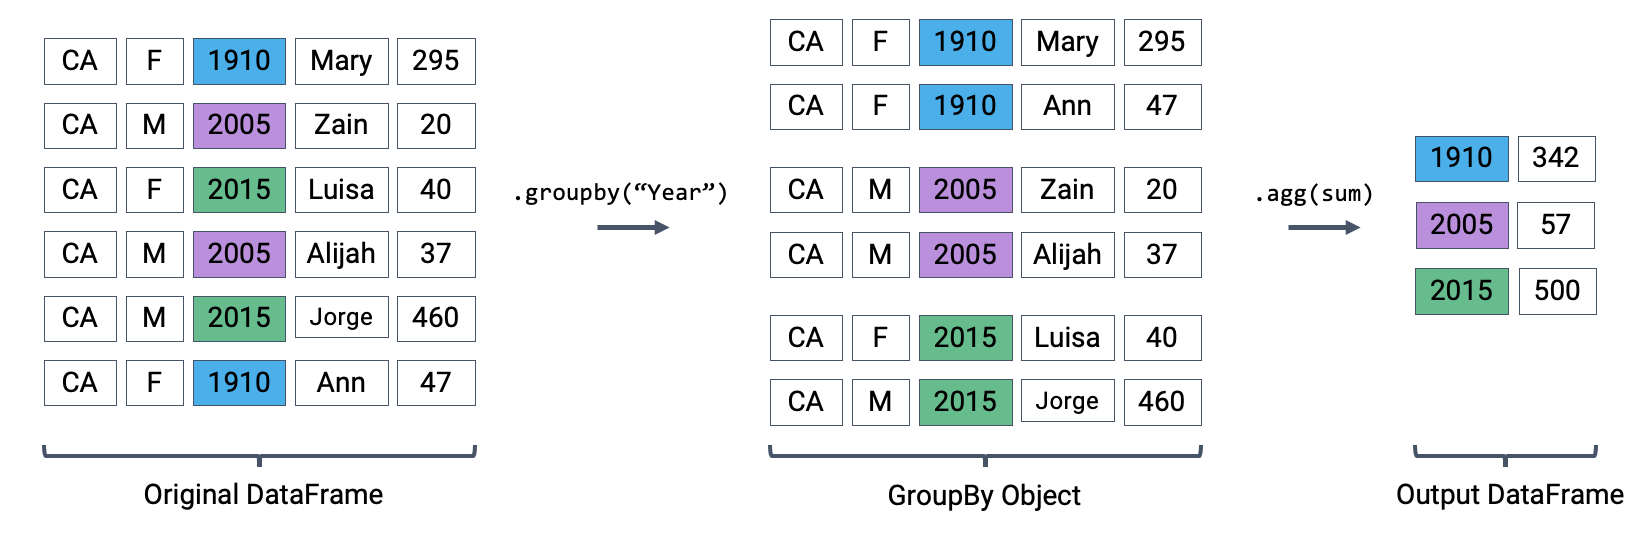
\includegraphics{pandas_3/images/agg.png}

}

\caption{Performing an aggregation}

\end{figure}%

Calling \texttt{.agg} has condensed each subframe back into a single
row. This gives us our final output: a \texttt{DataFrame} that is now
indexed by \texttt{"Year"}, with a single row for each unique year in
the original \texttt{babynames} DataFrame.

There are many different aggregation functions we can use, all of which
are useful in different applications.

\begin{Shaded}
\begin{Highlighting}[]
\NormalTok{babynames[[}\StringTok{"Year"}\NormalTok{, }\StringTok{"Count"}\NormalTok{]].groupby(}\StringTok{"Year"}\NormalTok{).agg(}\BuiltInTok{min}\NormalTok{).head(}\DecValTok{5}\NormalTok{)}
\end{Highlighting}
\end{Shaded}

\begin{verbatim}
C:\Users\yashd\AppData\Local\Temp\ipykernel_17528\86785752.py:1: FutureWarning:

The provided callable <built-in function min> is currently using DataFrameGroupBy.min. In a future version of pandas, the provided callable will be used directly. To keep current behavior pass the string "min" instead.
\end{verbatim}

\begin{longtable}[]{@{}ll@{}}
\toprule\noalign{}
& Count \\
Year & \\
\midrule\noalign{}
\endhead
\bottomrule\noalign{}
\endlastfoot
1910 & 5 \\
1911 & 5 \\
1912 & 5 \\
1913 & 5 \\
1914 & 5 \\
\end{longtable}

\begin{Shaded}
\begin{Highlighting}[]
\NormalTok{babynames[[}\StringTok{"Year"}\NormalTok{, }\StringTok{"Count"}\NormalTok{]].groupby(}\StringTok{"Year"}\NormalTok{).agg(}\BuiltInTok{max}\NormalTok{).head(}\DecValTok{5}\NormalTok{)}
\end{Highlighting}
\end{Shaded}

\begin{verbatim}
C:\Users\yashd\AppData\Local\Temp\ipykernel_17528\3032256904.py:1: FutureWarning:

The provided callable <built-in function max> is currently using DataFrameGroupBy.max. In a future version of pandas, the provided callable will be used directly. To keep current behavior pass the string "max" instead.
\end{verbatim}

\begin{longtable}[]{@{}ll@{}}
\toprule\noalign{}
& Count \\
Year & \\
\midrule\noalign{}
\endhead
\bottomrule\noalign{}
\endlastfoot
1910 & 295 \\
1911 & 390 \\
1912 & 534 \\
1913 & 614 \\
1914 & 773 \\
\end{longtable}

\begin{Shaded}
\begin{Highlighting}[]
\CommentTok{\# Same result, but now we explicitly tell pandas to only consider the "Count" column when summing}
\NormalTok{babynames.groupby(}\StringTok{"Year"}\NormalTok{)[[}\StringTok{"Count"}\NormalTok{]].agg(}\BuiltInTok{sum}\NormalTok{).head(}\DecValTok{5}\NormalTok{)}
\end{Highlighting}
\end{Shaded}

\begin{verbatim}
C:\Users\yashd\AppData\Local\Temp\ipykernel_17528\1958904241.py:2: FutureWarning:

The provided callable <built-in function sum> is currently using DataFrameGroupBy.sum. In a future version of pandas, the provided callable will be used directly. To keep current behavior pass the string "sum" instead.
\end{verbatim}

\begin{longtable}[]{@{}ll@{}}
\toprule\noalign{}
& Count \\
Year & \\
\midrule\noalign{}
\endhead
\bottomrule\noalign{}
\endlastfoot
1910 & 9163 \\
1911 & 9983 \\
1912 & 17946 \\
1913 & 22094 \\
1914 & 26926 \\
\end{longtable}

There are many different aggregations that can be applied to the grouped
data. The primary requirement is that an aggregation function must:

\begin{itemize}
\tightlist
\item
  Take in a \texttt{Series} of data (a single column of the grouped
  subframe).
\item
  Return a single value that aggregates this \texttt{Series}.
\end{itemize}

\subsection{Aggregation Functions}\label{aggregation-functions}

Because of this fairly broad requirement, \texttt{pandas} offers many
ways of computing an aggregation.

\textbf{In-built} Python operations -- such as \texttt{sum},
\texttt{max}, and \texttt{min} -- are automatically recognized by
\texttt{pandas}.

\begin{Shaded}
\begin{Highlighting}[]
\CommentTok{\# What is the minimum count for each name in any year?}
\NormalTok{babynames.groupby(}\StringTok{"Name"}\NormalTok{)[[}\StringTok{"Count"}\NormalTok{]].agg(}\BuiltInTok{min}\NormalTok{).head()}
\end{Highlighting}
\end{Shaded}

\begin{verbatim}
C:\Users\yashd\AppData\Local\Temp\ipykernel_17528\3244314896.py:2: FutureWarning:

The provided callable <built-in function min> is currently using DataFrameGroupBy.min. In a future version of pandas, the provided callable will be used directly. To keep current behavior pass the string "min" instead.
\end{verbatim}

\begin{longtable}[]{@{}ll@{}}
\toprule\noalign{}
& Count \\
Name & \\
\midrule\noalign{}
\endhead
\bottomrule\noalign{}
\endlastfoot
Aadan & 5 \\
Aadarsh & 6 \\
Aaden & 10 \\
Aadhav & 6 \\
Aadhini & 6 \\
\end{longtable}

\begin{Shaded}
\begin{Highlighting}[]
\CommentTok{\# What is the largest single{-}year count of each name?}
\NormalTok{babynames.groupby(}\StringTok{"Name"}\NormalTok{)[[}\StringTok{"Count"}\NormalTok{]].agg(}\BuiltInTok{max}\NormalTok{).head()}
\end{Highlighting}
\end{Shaded}

\begin{verbatim}
C:\Users\yashd\AppData\Local\Temp\ipykernel_17528\3805876622.py:2: FutureWarning:

The provided callable <built-in function max> is currently using DataFrameGroupBy.max. In a future version of pandas, the provided callable will be used directly. To keep current behavior pass the string "max" instead.
\end{verbatim}

\begin{longtable}[]{@{}ll@{}}
\toprule\noalign{}
& Count \\
Name & \\
\midrule\noalign{}
\endhead
\bottomrule\noalign{}
\endlastfoot
Aadan & 7 \\
Aadarsh & 6 \\
Aaden & 158 \\
Aadhav & 8 \\
Aadhini & 6 \\
\end{longtable}

As mentioned previously, functions from the \texttt{NumPy} library, such
as \texttt{np.mean}, \texttt{np.max}, \texttt{np.min}, and
\texttt{np.sum}, are also fair game in \texttt{pandas}.

\begin{Shaded}
\begin{Highlighting}[]
\CommentTok{\# What is the average count for each name across all years?}
\NormalTok{babynames.groupby(}\StringTok{"Name"}\NormalTok{)[[}\StringTok{"Count"}\NormalTok{]].agg(np.mean).head()}
\end{Highlighting}
\end{Shaded}

\begin{verbatim}
C:\Users\yashd\AppData\Local\Temp\ipykernel_17528\308986604.py:2: FutureWarning:

The provided callable <function mean at 0x000001BE5AA29300> is currently using DataFrameGroupBy.mean. In a future version of pandas, the provided callable will be used directly. To keep current behavior pass the string "mean" instead.
\end{verbatim}

\begin{longtable}[]{@{}ll@{}}
\toprule\noalign{}
& Count \\
Name & \\
\midrule\noalign{}
\endhead
\bottomrule\noalign{}
\endlastfoot
Aadan & 6.000000 \\
Aadarsh & 6.000000 \\
Aaden & 46.214286 \\
Aadhav & 6.750000 \\
Aadhini & 6.000000 \\
\end{longtable}

\texttt{pandas} also offers a number of in-built functions. Functions
that are native to \texttt{pandas} can be referenced using their string
name within a call to \texttt{.agg}. Some examples include:

\begin{itemize}
\tightlist
\item
  \texttt{.agg("sum")}
\item
  \texttt{.agg("max")}
\item
  \texttt{.agg("min")}
\item
  \texttt{.agg("mean")}
\item
  \texttt{.agg("first")}
\item
  \texttt{.agg("last")}
\end{itemize}

The latter two entries in this list -- \texttt{"first"} and
\texttt{"last"} -- are unique to \texttt{pandas}. They return the first
or last entry in a subframe column. Why might this be useful? Consider a
case where \emph{multiple} columns in a group share identical
information. To represent this information in the grouped output, we can
simply grab the first or last entry, which we know will be identical to
all other entries.

Let's illustrate this with an example. Say we add a new column to
\texttt{babynames} that contains the first letter of each name.

\begin{Shaded}
\begin{Highlighting}[]
\CommentTok{\# Imagine we had an additional column, "First Letter". We\textquotesingle{}ll explain this code next week}
\NormalTok{babynames[}\StringTok{"First Letter"}\NormalTok{] }\OperatorTok{=}\NormalTok{ babynames[}\StringTok{"Name"}\NormalTok{].}\BuiltInTok{str}\NormalTok{[}\DecValTok{0}\NormalTok{]}

\CommentTok{\# We construct a simplified DataFrame containing just a subset of columns}
\NormalTok{babynames\_new }\OperatorTok{=}\NormalTok{ babynames[[}\StringTok{"Name"}\NormalTok{, }\StringTok{"First Letter"}\NormalTok{, }\StringTok{"Year"}\NormalTok{]]}
\NormalTok{babynames\_new.head()}
\end{Highlighting}
\end{Shaded}

\begin{longtable}[]{@{}llll@{}}
\toprule\noalign{}
& Name & First Letter & Year \\
\midrule\noalign{}
\endhead
\bottomrule\noalign{}
\endlastfoot
115957 & Deandrea & D & 1990 \\
101976 & Deandrea & D & 1986 \\
131029 & Leandrea & L & 1994 \\
108731 & Deandrea & D & 1988 \\
308131 & Deandrea & D & 1985 \\
\end{longtable}

If we form groups for each name in the dataset, \texttt{"First\ Letter"}
will be the same for all members of the group. This means that if we
simply select the first entry for \texttt{"First\ Letter"} in the group,
we'll represent all data in that group.

We can use a dictionary to apply different aggregation functions to each
column during grouping.

\begin{figure}[H]

{\centering 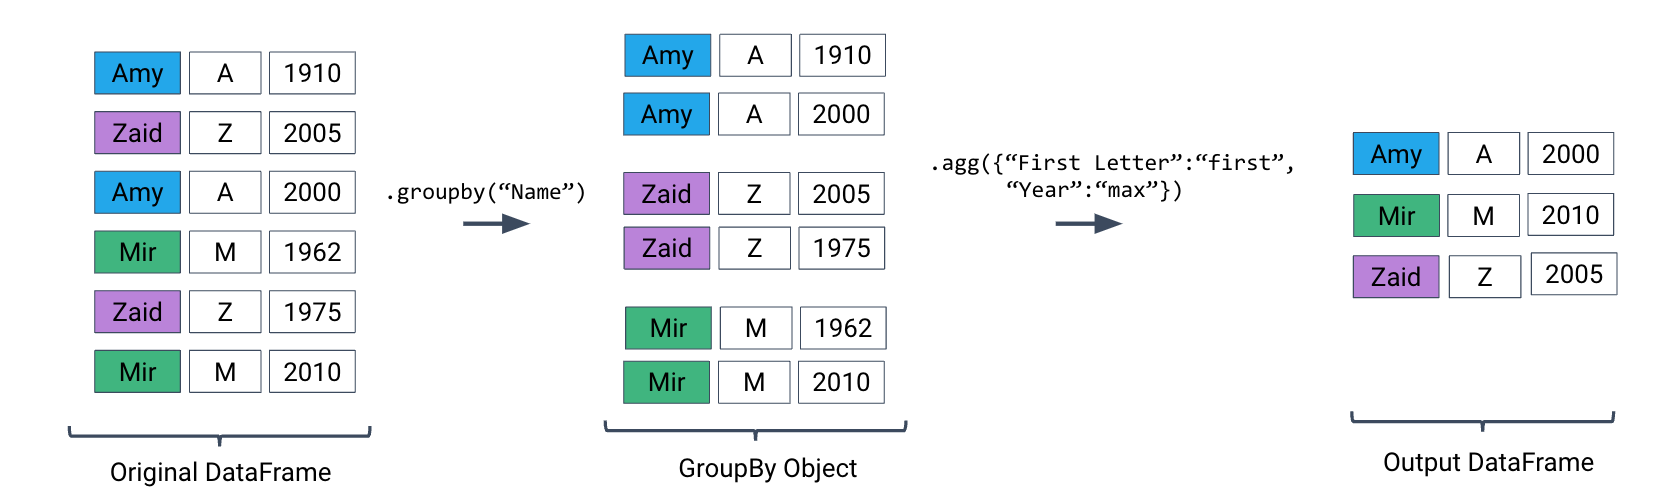
\includegraphics{pandas_3/images/first.png}

}

\caption{Aggregating using ``first''}

\end{figure}%

\begin{Shaded}
\begin{Highlighting}[]
\NormalTok{babynames\_new.groupby(}\StringTok{"Name"}\NormalTok{).agg(\{}\StringTok{"First Letter"}\NormalTok{:}\StringTok{"first"}\NormalTok{, }\StringTok{"Year"}\NormalTok{:}\StringTok{"max"}\NormalTok{\}).head()}
\end{Highlighting}
\end{Shaded}

\begin{longtable}[]{@{}lll@{}}
\toprule\noalign{}
& First Letter & Year \\
Name & & \\
\midrule\noalign{}
\endhead
\bottomrule\noalign{}
\endlastfoot
Aadan & A & 2014 \\
Aadarsh & A & 2019 \\
Aaden & A & 2020 \\
Aadhav & A & 2019 \\
Aadhini & A & 2022 \\
\end{longtable}

\subsection{Plotting Birth Counts}\label{plotting-birth-counts}

Let's use \texttt{.agg} to find the total number of babies born in each
year. Recall that using \texttt{.agg} with \texttt{.groupby()} follows
the format:
\texttt{df.groupby(column\_name).agg(aggregation\_function)}. The line
of code below gives us the total number of babies born in each year.

\begin{Shaded}
\begin{Highlighting}[]
\NormalTok{babynames.groupby(}\StringTok{"Year"}\NormalTok{)[[}\StringTok{"Count"}\NormalTok{]].agg(}\BuiltInTok{sum}\NormalTok{).head(}\DecValTok{5}\NormalTok{)}
\CommentTok{\# Alternative 1}
\CommentTok{\# babynames.groupby("Year")[["Count"]].sum()}
\CommentTok{\# Alternative 2}
\CommentTok{\# babynames.groupby("Year").sum(numeric\_only=True)}
\end{Highlighting}
\end{Shaded}

\begin{verbatim}
C:\Users\yashd\AppData\Local\Temp\ipykernel_17528\390646742.py:1: FutureWarning:

The provided callable <built-in function sum> is currently using DataFrameGroupBy.sum. In a future version of pandas, the provided callable will be used directly. To keep current behavior pass the string "sum" instead.
\end{verbatim}

\begin{longtable}[]{@{}ll@{}}
\toprule\noalign{}
& Count \\
Year & \\
\midrule\noalign{}
\endhead
\bottomrule\noalign{}
\endlastfoot
1910 & 9163 \\
1911 & 9983 \\
1912 & 17946 \\
1913 & 22094 \\
1914 & 26926 \\
\end{longtable}

Here's an illustration of the process:

Plotting the \texttt{Dataframe} we obtain tells an interesting story.

\begin{Shaded}
\begin{Highlighting}[]
\ImportTok{import}\NormalTok{ plotly.express }\ImportTok{as}\NormalTok{ px}
\NormalTok{puzzle2 }\OperatorTok{=}\NormalTok{ babynames.groupby(}\StringTok{"Year"}\NormalTok{)[[}\StringTok{"Count"}\NormalTok{]].agg(}\BuiltInTok{sum}\NormalTok{)}
\NormalTok{px.line(puzzle2, y }\OperatorTok{=} \StringTok{"Count"}\NormalTok{)}
\end{Highlighting}
\end{Shaded}

\begin{verbatim}
C:\Users\yashd\AppData\Local\Temp\ipykernel_17528\4066413905.py:2: FutureWarning:

The provided callable <built-in function sum> is currently using DataFrameGroupBy.sum. In a future version of pandas, the provided callable will be used directly. To keep current behavior pass the string "sum" instead.
\end{verbatim}

\begin{verbatim}
Unable to display output for mime type(s): text/html
\end{verbatim}

\begin{verbatim}
Unable to display output for mime type(s): text/html
\end{verbatim}

\textbf{A word of warning}: we made an enormous assumption when we
decided to use this dataset to estimate birth rate. According to
\href{https://lao.ca.gov/LAOEconTax/Article/Detail/691}{this article
from the Legistlative Analyst Office}, the true number of babies born in
California in 2020 was 421,275. However, our plot shows 362,882 babies
------ what happened?

\subsection{\texorpdfstring{Summary of the \texttt{.groupby()}
Function}{Summary of the .groupby() Function}}\label{summary-of-the-.groupby-function}

A \texttt{groupby} operation involves some combination of
\textbf{splitting a \texttt{DataFrame} into grouped subframes},
\textbf{applying a function}, and \textbf{combining the results}.

For some arbitrary \texttt{DataFrame} \texttt{df} below, the code
\texttt{df.groupby("year").agg(sum)} does the following:

\begin{itemize}
\tightlist
\item
  \textbf{Splits} the \texttt{DataFrame} into sub-\texttt{DataFrame}s
  with rows belonging to the same year.
\item
  \textbf{Applies} the \texttt{sum} function to each column of each
  sub-\texttt{DataFrame}.
\item
  \textbf{Combines} the results of \texttt{sum} into a single
  \texttt{DataFrame}, indexed by \texttt{year}.
\end{itemize}

\subsection{\texorpdfstring{Revisiting the \texttt{.agg()}
Function}{Revisiting the .agg() Function}}\label{revisiting-the-.agg-function}

\texttt{.agg()} can take in any function that aggregates several values
into one summary value. Some commonly-used aggregation functions can
even be called directly, without explicit use of \texttt{.agg()}. For
example, we can call \texttt{.mean()} on \texttt{.groupby()}:

\begin{verbatim}
babynames.groupby("Year").mean().head()
\end{verbatim}

We can now put this all into practice. Say we want to find the baby name
with sex ``F'' that has fallen in popularity the most in California. To
calculate this, we can first create a metric: ``Ratio to Peak'' (RTP).
The RTP is the ratio of babies born with a given name in 2022 to the
\emph{maximum} number of babies born with the name in \emph{any} year.

Let's start with calculating this for one baby, ``Jennifer''.

\begin{Shaded}
\begin{Highlighting}[]
\CommentTok{\# We filter by babies with sex "F" and sort by "Year"}
\NormalTok{f\_babynames }\OperatorTok{=}\NormalTok{ babynames[babynames[}\StringTok{"Sex"}\NormalTok{] }\OperatorTok{==} \StringTok{"F"}\NormalTok{]}
\NormalTok{f\_babynames }\OperatorTok{=}\NormalTok{ f\_babynames.sort\_values([}\StringTok{"Year"}\NormalTok{])}

\CommentTok{\# Determine how many Jennifers were born in CA per year}
\NormalTok{jenn\_counts\_series }\OperatorTok{=}\NormalTok{ f\_babynames[f\_babynames[}\StringTok{"Name"}\NormalTok{] }\OperatorTok{==} \StringTok{"Jennifer"}\NormalTok{][}\StringTok{"Count"}\NormalTok{]}

\CommentTok{\# Determine the max number of Jennifers born in a year and the number born in 2022 }
\CommentTok{\# to calculate RTP}
\NormalTok{max\_jenn }\OperatorTok{=} \BuiltInTok{max}\NormalTok{(f\_babynames[f\_babynames[}\StringTok{"Name"}\NormalTok{] }\OperatorTok{==} \StringTok{"Jennifer"}\NormalTok{][}\StringTok{"Count"}\NormalTok{])}
\NormalTok{curr\_jenn }\OperatorTok{=}\NormalTok{ f\_babynames[f\_babynames[}\StringTok{"Name"}\NormalTok{] }\OperatorTok{==} \StringTok{"Jennifer"}\NormalTok{][}\StringTok{"Count"}\NormalTok{].iloc[}\OperatorTok{{-}}\DecValTok{1}\NormalTok{]}
\NormalTok{rtp }\OperatorTok{=}\NormalTok{ curr\_jenn }\OperatorTok{/}\NormalTok{ max\_jenn}
\NormalTok{rtp}
\end{Highlighting}
\end{Shaded}

\begin{verbatim}
0.018796372629843364
\end{verbatim}

By creating a function to calculate RTP and applying it to our
\texttt{DataFrame} by using \texttt{.groupby()}, we can easily compute
the RTP for all names at once!

\begin{Shaded}
\begin{Highlighting}[]
\KeywordTok{def}\NormalTok{ ratio\_to\_peak(series):}
    \ControlFlowTok{return}\NormalTok{ series.iloc[}\OperatorTok{{-}}\DecValTok{1}\NormalTok{] }\OperatorTok{/} \BuiltInTok{max}\NormalTok{(series)}

\CommentTok{\#Using .groupby() to apply the function}
\NormalTok{rtp\_table }\OperatorTok{=}\NormalTok{ f\_babynames.groupby(}\StringTok{"Name"}\NormalTok{)[[}\StringTok{"Year"}\NormalTok{, }\StringTok{"Count"}\NormalTok{]].agg(ratio\_to\_peak)}
\NormalTok{rtp\_table.head()}
\end{Highlighting}
\end{Shaded}

\begin{longtable}[]{@{}lll@{}}
\toprule\noalign{}
& Year & Count \\
Name & & \\
\midrule\noalign{}
\endhead
\bottomrule\noalign{}
\endlastfoot
Aadhini & 1.0 & 1.000000 \\
Aadhira & 1.0 & 0.500000 \\
Aadhya & 1.0 & 0.660000 \\
Aadya & 1.0 & 0.586207 \\
Aahana & 1.0 & 0.269231 \\
\end{longtable}

In the rows shown above, we can see that every row shown has a
\texttt{Year} value of \texttt{1.0}.

This is the ``\textbf{\texttt{pandas}}-ification'' of logic you saw in
Data 8. Much of the logic you've learned in Data 8 will serve you well
in Data 100.

\subsection{Nuisance Columns}\label{nuisance-columns}

Note that you must be careful with which columns you apply the
\texttt{.agg()} function to. If we were to apply our function to the
table as a whole by doing
\texttt{f\_babynames.groupby("Name").agg(ratio\_to\_peak)}, executing
our \texttt{.agg()} call would result in a \texttt{TypeError}.

We can avoid this issue (and prevent unintentional loss of data) by
explicitly selecting column(s) we want to apply our aggregation function
to \textbf{BEFORE} calling \texttt{.agg()},

\subsection{Renaming Columns After
Grouping}\label{renaming-columns-after-grouping}

By default, \texttt{.groupby} will not rename any aggregated columns. As
we can see in the table above, the aggregated column is still named
\texttt{Count} even though it now represents the RTP. For better
readability, we can rename \texttt{Count} to \texttt{Count\ RTP}

\begin{Shaded}
\begin{Highlighting}[]
\NormalTok{rtp\_table }\OperatorTok{=}\NormalTok{ rtp\_table.rename(columns }\OperatorTok{=}\NormalTok{ \{}\StringTok{"Count"}\NormalTok{: }\StringTok{"Count RTP"}\NormalTok{\})}
\NormalTok{rtp\_table}
\end{Highlighting}
\end{Shaded}

\begin{longtable}[]{@{}lll@{}}
\toprule\noalign{}
& Year & Count RTP \\
Name & & \\
\midrule\noalign{}
\endhead
\bottomrule\noalign{}
\endlastfoot
Aadhini & 1.0 & 1.000000 \\
Aadhira & 1.0 & 0.500000 \\
Aadhya & 1.0 & 0.660000 \\
Aadya & 1.0 & 0.586207 \\
Aahana & 1.0 & 0.269231 \\
... & ... & ... \\
Zyanya & 1.0 & 0.466667 \\
Zyla & 1.0 & 1.000000 \\
Zylah & 1.0 & 1.000000 \\
Zyra & 1.0 & 1.000000 \\
Zyrah & 1.0 & 0.833333 \\
\end{longtable}

\subsection{Some Data Science Payoff}\label{some-data-science-payoff}

By sorting \texttt{rtp\_table}, we can see the names whose popularity
has decreased the most.

\begin{Shaded}
\begin{Highlighting}[]
\NormalTok{rtp\_table }\OperatorTok{=}\NormalTok{ rtp\_table.rename(columns }\OperatorTok{=}\NormalTok{ \{}\StringTok{"Count"}\NormalTok{: }\StringTok{"Count RTP"}\NormalTok{\})}
\NormalTok{rtp\_table.sort\_values(}\StringTok{"Count RTP"}\NormalTok{).head()}
\end{Highlighting}
\end{Shaded}

\begin{longtable}[]{@{}lll@{}}
\toprule\noalign{}
& Year & Count RTP \\
Name & & \\
\midrule\noalign{}
\endhead
\bottomrule\noalign{}
\endlastfoot
Debra & 1.0 & 0.001260 \\
Debbie & 1.0 & 0.002815 \\
Carol & 1.0 & 0.003180 \\
Tammy & 1.0 & 0.003249 \\
Susan & 1.0 & 0.003305 \\
\end{longtable}

To visualize the above \texttt{DataFrame}, let's look at the line plot
below:

\begin{Shaded}
\begin{Highlighting}[]
\ImportTok{import}\NormalTok{ plotly.express }\ImportTok{as}\NormalTok{ px}
\NormalTok{px.line(f\_babynames[f\_babynames[}\StringTok{"Name"}\NormalTok{] }\OperatorTok{==} \StringTok{"Debra"}\NormalTok{], x }\OperatorTok{=} \StringTok{"Year"}\NormalTok{, y }\OperatorTok{=} \StringTok{"Count"}\NormalTok{)}
\end{Highlighting}
\end{Shaded}

\begin{verbatim}
Unable to display output for mime type(s): text/html
\end{verbatim}

We can get the list of the top 10 names and then plot popularity with
the following code:

\begin{Shaded}
\begin{Highlighting}[]
\NormalTok{top10 }\OperatorTok{=}\NormalTok{ rtp\_table.sort\_values(}\StringTok{"Count RTP"}\NormalTok{).head(}\DecValTok{10}\NormalTok{).index}
\NormalTok{px.line(}
\NormalTok{    f\_babynames[f\_babynames[}\StringTok{"Name"}\NormalTok{].isin(top10)], }
\NormalTok{    x }\OperatorTok{=} \StringTok{"Year"}\NormalTok{, }
\NormalTok{    y }\OperatorTok{=} \StringTok{"Count"}\NormalTok{, }
\NormalTok{    color }\OperatorTok{=} \StringTok{"Name"}
\NormalTok{)}
\end{Highlighting}
\end{Shaded}

\begin{verbatim}
C:\Users\yashd\AppData\Local\Programs\Python\Python312\Lib\site-packages\plotly\express\_core.py:2065: FutureWarning:

When grouping with a length-1 list-like, you will need to pass a length-1 tuple to get_group in a future version of pandas. Pass `(name,)` instead of `name` to silence this warning.
\end{verbatim}

\begin{verbatim}
Unable to display output for mime type(s): text/html
\end{verbatim}

As a quick exercise, consider what code would compute the total number
of babies with each name.

\begin{Shaded}
\begin{Highlighting}[]
\NormalTok{babynames.groupby(}\StringTok{"Name"}\NormalTok{)[[}\StringTok{"Count"}\NormalTok{]].agg(}\BuiltInTok{sum}\NormalTok{).head()}
\CommentTok{\# alternative solution: }
\CommentTok{\# babynames.groupby("Name")[["Count"]].sum()}
\end{Highlighting}
\end{Shaded}

\begin{verbatim}
C:\Users\yashd\AppData\Local\Temp\ipykernel_17528\1912269730.py:1: FutureWarning:

The provided callable <built-in function sum> is currently using DataFrameGroupBy.sum. In a future version of pandas, the provided callable will be used directly. To keep current behavior pass the string "sum" instead.
\end{verbatim}

\begin{longtable}[]{@{}ll@{}}
\toprule\noalign{}
& Count \\
Name & \\
\midrule\noalign{}
\endhead
\bottomrule\noalign{}
\endlastfoot
Aadan & 18 \\
Aadarsh & 6 \\
Aaden & 647 \\
Aadhav & 27 \\
Aadhini & 6 \\
\end{longtable}

\section{\texorpdfstring{\texttt{.groupby()},
Continued}{.groupby(), Continued}}\label{groupby-continued}

We'll work with the \texttt{elections} \texttt{DataFrame} again.

\begin{Shaded}
\begin{Highlighting}[]
\ImportTok{import}\NormalTok{ pandas }\ImportTok{as}\NormalTok{ pd}
\ImportTok{import}\NormalTok{ numpy }\ImportTok{as}\NormalTok{ np}

\NormalTok{elections }\OperatorTok{=}\NormalTok{ pd.read\_csv(}\StringTok{"data/elections.csv"}\NormalTok{)}
\NormalTok{elections.head(}\DecValTok{5}\NormalTok{)}
\end{Highlighting}
\end{Shaded}

\begin{longtable}[]{@{}lllllll@{}}
\toprule\noalign{}
& Year & Candidate & Party & Popular vote & Result & \% \\
\midrule\noalign{}
\endhead
\bottomrule\noalign{}
\endlastfoot
0 & 1824 & Andrew Jackson & Democratic-Republican & 151271 & loss &
57.210122 \\
1 & 1824 & John Quincy Adams & Democratic-Republican & 113142 & win &
42.789878 \\
2 & 1828 & Andrew Jackson & Democratic & 642806 & win & 56.203927 \\
3 & 1828 & John Quincy Adams & National Republican & 500897 & loss &
43.796073 \\
4 & 1832 & Andrew Jackson & Democratic & 702735 & win & 54.574789 \\
\end{longtable}

\subsection{\texorpdfstring{Raw \texttt{GroupBy}
Objects}{Raw GroupBy Objects}}\label{raw-groupby-objects}

The result of \texttt{groupby} applied to a \texttt{DataFrame} is a
\texttt{DataFrameGroupBy} object, \textbf{not} a \texttt{DataFrame}.

\begin{Shaded}
\begin{Highlighting}[]
\NormalTok{grouped\_by\_year }\OperatorTok{=}\NormalTok{ elections.groupby(}\StringTok{"Year"}\NormalTok{)}
\BuiltInTok{type}\NormalTok{(grouped\_by\_year)}
\end{Highlighting}
\end{Shaded}

\begin{verbatim}
pandas.core.groupby.generic.DataFrameGroupBy
\end{verbatim}

There are several ways to look into \texttt{DataFrameGroupBy} objects:

\begin{Shaded}
\begin{Highlighting}[]
\NormalTok{grouped\_by\_party }\OperatorTok{=}\NormalTok{ elections.groupby(}\StringTok{"Party"}\NormalTok{)}
\NormalTok{grouped\_by\_party.groups}
\end{Highlighting}
\end{Shaded}

\begin{verbatim}
{'American': [22, 126], 'American Independent': [115, 119, 124], 'Anti-Masonic': [6], 'Anti-Monopoly': [38], 'Citizens': [127], 'Communist': [89], 'Constitution': [160, 164, 172], 'Constitutional Union': [24], 'Democratic': [2, 4, 8, 10, 13, 14, 17, 20, 28, 29, 34, 37, 39, 45, 47, 52, 55, 57, 64, 70, 74, 77, 81, 83, 86, 91, 94, 97, 100, 105, 108, 111, 114, 116, 118, 123, 129, 134, 137, 140, 144, 151, 158, 162, 168, 176, 178], 'Democratic-Republican': [0, 1], 'Dixiecrat': [103], 'Farmer–Labor': [78], 'Free Soil': [15, 18], 'Green': [149, 155, 156, 165, 170, 177, 181], 'Greenback': [35], 'Independent': [121, 130, 143, 161, 167, 174], 'Liberal Republican': [31], 'Libertarian': [125, 128, 132, 138, 139, 146, 153, 159, 163, 169, 175, 180], 'National Democratic': [50], 'National Republican': [3, 5], 'National Union': [27], 'Natural Law': [148], 'New Alliance': [136], 'Northern Democratic': [26], 'Populist': [48, 61, 141], 'Progressive': [68, 82, 101, 107], 'Prohibition': [41, 44, 49, 51, 54, 59, 63, 67, 73, 75, 99], 'Reform': [150, 154], 'Republican': [21, 23, 30, 32, 33, 36, 40, 43, 46, 53, 56, 60, 65, 69, 72, 79, 80, 84, 87, 90, 96, 98, 104, 106, 109, 112, 113, 117, 120, 122, 131, 133, 135, 142, 145, 152, 157, 166, 171, 173, 179], 'Socialist': [58, 62, 66, 71, 76, 85, 88, 92, 95, 102], 'Southern Democratic': [25], 'States' Rights': [110], 'Taxpayers': [147], 'Union': [93], 'Union Labor': [42], 'Whig': [7, 9, 11, 12, 16, 19]}
\end{verbatim}

\begin{Shaded}
\begin{Highlighting}[]
\NormalTok{grouped\_by\_party.get\_group(}\StringTok{"Socialist"}\NormalTok{)}
\end{Highlighting}
\end{Shaded}

\begin{longtable}[]{@{}lllllll@{}}
\toprule\noalign{}
& Year & Candidate & Party & Popular vote & Result & \% \\
\midrule\noalign{}
\endhead
\bottomrule\noalign{}
\endlastfoot
58 & 1904 & Eugene V. Debs & Socialist & 402810 & loss & 2.985897 \\
62 & 1908 & Eugene V. Debs & Socialist & 420852 & loss & 2.850866 \\
66 & 1912 & Eugene V. Debs & Socialist & 901551 & loss & 6.004354 \\
71 & 1916 & Allan L. Benson & Socialist & 590524 & loss & 3.194193 \\
76 & 1920 & Eugene V. Debs & Socialist & 913693 & loss & 3.428282 \\
85 & 1928 & Norman Thomas & Socialist & 267478 & loss & 0.728623 \\
88 & 1932 & Norman Thomas & Socialist & 884885 & loss & 2.236211 \\
92 & 1936 & Norman Thomas & Socialist & 187910 & loss & 0.412876 \\
95 & 1940 & Norman Thomas & Socialist & 116599 & loss & 0.234237 \\
102 & 1948 & Norman Thomas & Socialist & 139569 & loss & 0.286312 \\
\end{longtable}

\subsection{\texorpdfstring{Other \texttt{GroupBy}
Methods}{Other GroupBy Methods}}\label{other-groupby-methods}

There are many aggregation methods we can use with \texttt{.agg}. Some
useful options are:

\begin{itemize}
\tightlist
\item
  \href{https://pandas.pydata.org/docs/reference/api/pandas.core.groupby.DataFrameGroupBy.mean.html\#pandas.core.groupby.DataFrameGroupBy.mean}{\texttt{.mean}}:
  creates a new \texttt{DataFrame} with the mean value of each group
\item
  \href{https://pandas.pydata.org/docs/reference/api/pandas.core.groupby.DataFrameGroupBy.sum.html\#pandas.core.groupby.DataFrameGroupBy.sum}{\texttt{.sum}}:
  creates a new \texttt{DataFrame} with the sum of each group
\item
  \href{https://pandas.pydata.org/docs/reference/api/pandas.core.groupby.DataFrameGroupBy.max.html\#pandas.core.groupby.DataFrameGroupBy.max}{\texttt{.max}}
  and
  \href{https://pandas.pydata.org/docs/reference/api/pandas.core.groupby.DataFrameGroupBy.min.html\#pandas.core.groupby.DataFrameGroupBy.min}{\texttt{.min}}:
  creates a new \texttt{DataFrame} with the maximum/minimum value of
  each group
\item
  \href{https://pandas.pydata.org/docs/reference/api/pandas.core.groupby.DataFrameGroupBy.first.html\#pandas.core.groupby.DataFrameGroupBy.first}{\texttt{.first}}
  and
  \href{https://pandas.pydata.org/docs/reference/api/pandas.core.groupby.DataFrameGroupBy.last.html\#pandas.core.groupby.DataFrameGroupBy.last}{\texttt{.last}}:
  creates a new \texttt{DataFrame} with the first/last row in each group
\item
  \href{https://pandas.pydata.org/docs/reference/api/pandas.core.groupby.DataFrameGroupBy.size.html\#pandas.core.groupby.DataFrameGroupBy.size}{\texttt{.size}}:
  creates a new \textbf{\texttt{Series}} with the number of entries in
  each group
\item
  \href{https://pandas.pydata.org/docs/reference/api/pandas.core.groupby.DataFrameGroupBy.count.html\#pandas.core.groupby.DataFrameGroupBy.count}{\texttt{.count}}:
  creates a new \textbf{\texttt{DataFrame}} with the number of entries,
  excluding missing values.
\end{itemize}

Let's illustrate some examples by creating a \texttt{DataFrame} called
\texttt{df}.

\begin{Shaded}
\begin{Highlighting}[]
\NormalTok{df }\OperatorTok{=}\NormalTok{ pd.DataFrame(\{}\StringTok{\textquotesingle{}letter\textquotesingle{}}\NormalTok{:[}\StringTok{\textquotesingle{}A\textquotesingle{}}\NormalTok{,}\StringTok{\textquotesingle{}A\textquotesingle{}}\NormalTok{,}\StringTok{\textquotesingle{}B\textquotesingle{}}\NormalTok{,}\StringTok{\textquotesingle{}C\textquotesingle{}}\NormalTok{,}\StringTok{\textquotesingle{}C\textquotesingle{}}\NormalTok{,}\StringTok{\textquotesingle{}C\textquotesingle{}}\NormalTok{], }
                   \StringTok{\textquotesingle{}num\textquotesingle{}}\NormalTok{:[}\DecValTok{1}\NormalTok{,}\DecValTok{2}\NormalTok{,}\DecValTok{3}\NormalTok{,}\DecValTok{4}\NormalTok{,np.NaN,}\DecValTok{4}\NormalTok{], }
                   \StringTok{\textquotesingle{}state\textquotesingle{}}\NormalTok{:[np.NaN, }\StringTok{\textquotesingle{}tx\textquotesingle{}}\NormalTok{, }\StringTok{\textquotesingle{}fl\textquotesingle{}}\NormalTok{, }\StringTok{\textquotesingle{}hi\textquotesingle{}}\NormalTok{, np.NaN, }\StringTok{\textquotesingle{}ak\textquotesingle{}}\NormalTok{]\})}
\NormalTok{df}
\end{Highlighting}
\end{Shaded}

\begin{longtable}[]{@{}llll@{}}
\toprule\noalign{}
& letter & num & state \\
\midrule\noalign{}
\endhead
\bottomrule\noalign{}
\endlastfoot
0 & A & 1.0 & NaN \\
1 & A & 2.0 & tx \\
2 & B & 3.0 & fl \\
3 & C & 4.0 & hi \\
4 & C & NaN & NaN \\
5 & C & 4.0 & ak \\
\end{longtable}

Note the slight difference between \texttt{.size()} and
\texttt{.count()}: while \texttt{.size()} returns a \texttt{Series} and
counts the number of entries including the missing values,
\texttt{.count()} returns a \texttt{DataFrame} and counts the number of
entries in each column \emph{excluding missing values}.

\begin{Shaded}
\begin{Highlighting}[]
\NormalTok{df.groupby(}\StringTok{"letter"}\NormalTok{).size()}
\end{Highlighting}
\end{Shaded}

\begin{verbatim}
letter
A    2
B    1
C    3
dtype: int64
\end{verbatim}

\begin{Shaded}
\begin{Highlighting}[]
\NormalTok{df.groupby(}\StringTok{"letter"}\NormalTok{).count()}
\end{Highlighting}
\end{Shaded}

\begin{longtable}[]{@{}lll@{}}
\toprule\noalign{}
& num & state \\
letter & & \\
\midrule\noalign{}
\endhead
\bottomrule\noalign{}
\endlastfoot
A & 2 & 1 \\
B & 1 & 1 \\
C & 2 & 2 \\
\end{longtable}

You might recall that the \texttt{value\_counts()} function in the
previous note does something similar. It turns out
\texttt{value\_counts()} and \texttt{groupby.size()} are the same,
except \texttt{value\_counts()} sorts the resulting \texttt{Series} in
descending order automatically.

\begin{Shaded}
\begin{Highlighting}[]
\NormalTok{df[}\StringTok{"letter"}\NormalTok{].value\_counts()}
\end{Highlighting}
\end{Shaded}

\begin{verbatim}
letter
C    3
A    2
B    1
Name: count, dtype: int64
\end{verbatim}

These (and other) aggregation functions are so common that
\texttt{pandas} allows for writing shorthand. Instead of explicitly
stating the use of \texttt{.agg}, we can call the function directly on
the \texttt{GroupBy} object.

For example, the following are equivalent:

\begin{itemize}
\tightlist
\item
  \texttt{elections.groupby("Candidate").agg(mean)}
\item
  \texttt{elections.groupby("Candidate").mean()}
\end{itemize}

There are many other methods that \texttt{pandas} supports. You can
check them out on the
\href{https://pandas.pydata.org/docs/reference/groupby.html}{\texttt{pandas}
documentation}.

\subsection{Filtering by Group}\label{filtering-by-group}

Another common use for \texttt{GroupBy} objects is to filter data by
group.

\texttt{groupby.filter} takes an argument \texttt{func}, where
\texttt{func} is a function that:

\begin{itemize}
\tightlist
\item
  Takes a \texttt{DataFrame} object as input
\item
  Returns a single \texttt{True} or \texttt{False}.
\end{itemize}

\texttt{groupby.filter} applies \texttt{func} to each
group/sub-\texttt{DataFrame}:

\begin{itemize}
\tightlist
\item
  If \texttt{func} returns \texttt{True} for a group, then all rows
  belonging to the group are preserved.
\item
  If \texttt{func} returns \texttt{False} for a group, then all rows
  belonging to that group are filtered out.
\end{itemize}

In other words, sub-\texttt{DataFrame}s that correspond to \texttt{True}
are returned in the final result, whereas those with a \texttt{False}
value are not. Importantly, \texttt{groupby.filter} is different from
\texttt{groupby.agg} in that an \emph{entire} sub-\texttt{DataFrame} is
returned in the final \texttt{DataFrame}, not just a single row. As a
result, \texttt{groupby.filter} preserves the original indices and the
column we grouped on does \textbf{NOT} become the index!

To illustrate how this happens, let's go back to the \texttt{elections}
dataset. Say we want to identify ``tight'' election years -- that is, we
want to find all rows that correspond to election years where all
candidates in that year won a similar portion of the total vote.
Specifically, let's find all rows corresponding to a year where no
candidate won more than 45\% of the total vote.

In other words, we want to:

\begin{itemize}
\tightlist
\item
  Find the years where the maximum \texttt{\%} in that year is less than
  45\%
\item
  Return all \texttt{DataFrame} rows that correspond to these years
\end{itemize}

For each year, we need to find the maximum \texttt{\%} among \emph{all}
rows for that year. If this maximum \texttt{\%} is lower than 45\%, we
will tell \texttt{pandas} to keep all rows corresponding to that year.

\begin{Shaded}
\begin{Highlighting}[]
\NormalTok{elections.groupby(}\StringTok{"Year"}\NormalTok{).}\BuiltInTok{filter}\NormalTok{(}\KeywordTok{lambda}\NormalTok{ sf: sf[}\StringTok{"\%"}\NormalTok{].}\BuiltInTok{max}\NormalTok{() }\OperatorTok{\textless{}} \DecValTok{45}\NormalTok{).head(}\DecValTok{9}\NormalTok{)}
\end{Highlighting}
\end{Shaded}

\begin{longtable}[]{@{}lllllll@{}}
\toprule\noalign{}
& Year & Candidate & Party & Popular vote & Result & \% \\
\midrule\noalign{}
\endhead
\bottomrule\noalign{}
\endlastfoot
23 & 1860 & Abraham Lincoln & Republican & 1855993 & win & 39.699408 \\
24 & 1860 & John Bell & Constitutional Union & 590901 & loss &
12.639283 \\
25 & 1860 & John C. Breckinridge & Southern Democratic & 848019 & loss &
18.138998 \\
26 & 1860 & Stephen A. Douglas & Northern Democratic & 1380202 & loss &
29.522311 \\
66 & 1912 & Eugene V. Debs & Socialist & 901551 & loss & 6.004354 \\
67 & 1912 & Eugene W. Chafin & Prohibition & 208156 & loss & 1.386325 \\
68 & 1912 & Theodore Roosevelt & Progressive & 4122721 & loss &
27.457433 \\
69 & 1912 & William Taft & Republican & 3486242 & loss & 23.218466 \\
70 & 1912 & Woodrow Wilson & Democratic & 6296284 & win & 41.933422 \\
\end{longtable}

What's going on here? In this example, we've defined our filtering
function, \texttt{func}, to be
\texttt{lambda\ sf:\ sf{[}"\%"{]}.max()\ \textless{}\ 45}. This
filtering function will find the maximum \texttt{"\%"} value among all
entries in the grouped sub-\texttt{DataFrame}, which we call
\texttt{sf}. If the maximum value is less than 45, then the filter
function will return \texttt{True} and all rows in that grouped
sub-\texttt{DataFrame} will appear in the final output
\texttt{DataFrame}.

Examine the \texttt{DataFrame} above. Notice how, in this preview of the
first 9 rows, all entries from the years 1860 and 1912 appear. This
means that in 1860 and 1912, no candidate in that year won more than
45\% of the total vote.

You may ask: how is the \texttt{groupby.filter} procedure different to
the boolean filtering we've seen previously? Boolean filtering considers
\emph{individual} rows when applying a boolean condition. For example,
the code \texttt{elections{[}elections{[}"\%"{]}\ \textless{}\ 45{]}}
will check the \texttt{"\%"} value of every single row in
\texttt{elections}; if it is less than 45, then that row will be kept in
the output. \texttt{groupby.filter}, in contrast, applies a boolean
condition \emph{across} all rows in a group. If not all rows in that
group satisfy the condition specified by the filter, the entire group
will be discarded in the output.

\subsection{\texorpdfstring{Aggregation with \texttt{lambda}
Functions}{Aggregation with lambda Functions}}\label{aggregation-with-lambda-functions}

What if we wish to aggregate our \texttt{DataFrame} using a non-standard
function -- for example, a function of our own design? We can do so by
combining \texttt{.agg} with \texttt{lambda} expressions.

Let's first consider a puzzle to jog our memory. We will attempt to find
the \texttt{Candidate} from each \texttt{Party} with the highest
\texttt{\%} of votes.

A naive approach may be to group by the \texttt{Party} column and
aggregate by the maximum.

\begin{Shaded}
\begin{Highlighting}[]
\NormalTok{elections.groupby(}\StringTok{"Party"}\NormalTok{).agg(}\BuiltInTok{max}\NormalTok{).head(}\DecValTok{10}\NormalTok{)}
\end{Highlighting}
\end{Shaded}

\begin{verbatim}
C:\Users\yashd\AppData\Local\Temp\ipykernel_17528\4278286395.py:1: FutureWarning:

The provided callable <built-in function max> is currently using DataFrameGroupBy.max. In a future version of pandas, the provided callable will be used directly. To keep current behavior pass the string "max" instead.
\end{verbatim}

\begin{longtable}[]{@{}llllll@{}}
\toprule\noalign{}
& Year & Candidate & Popular vote & Result & \% \\
Party & & & & & \\
\midrule\noalign{}
\endhead
\bottomrule\noalign{}
\endlastfoot
American & 1976 & Thomas J. Anderson & 873053 & loss & 21.554001 \\
American Independent & 1976 & Lester Maddox & 9901118 & loss &
13.571218 \\
Anti-Masonic & 1832 & William Wirt & 100715 & loss & 7.821583 \\
Anti-Monopoly & 1884 & Benjamin Butler & 134294 & loss & 1.335838 \\
Citizens & 1980 & Barry Commoner & 233052 & loss & 0.270182 \\
Communist & 1932 & William Z. Foster & 103307 & loss & 0.261069 \\
Constitution & 2016 & Michael Peroutka & 203091 & loss & 0.152398 \\
Constitutional Union & 1860 & John Bell & 590901 & loss & 12.639283 \\
Democratic & 2020 & Woodrow Wilson & 81268924 & win & 61.344703 \\
Democratic-Republican & 1824 & John Quincy Adams & 151271 & win &
57.210122 \\
\end{longtable}

This approach is clearly wrong -- the \texttt{DataFrame} claims that
Woodrow Wilson won the presidency in 2020.

Why is this happening? Here, the \texttt{max} aggregation function is
taken over every column \emph{independently}. Among Democrats,
\texttt{max} is computing:

\begin{itemize}
\tightlist
\item
  The most recent \texttt{Year} a Democratic candidate ran for president
  (2020)
\item
  The \texttt{Candidate} with the alphabetically ``largest'' name
  (``Woodrow Wilson'')
\item
  The \texttt{Result} with the alphabetically ``largest'' outcome
  (``win'')
\end{itemize}

Instead, let's try a different approach. We will:

\begin{enumerate}
\def\labelenumi{\arabic{enumi}.}
\tightlist
\item
  Sort the \texttt{DataFrame} so that rows are in descending order of
  \texttt{\%}
\item
  Group by \texttt{Party} and select the first row of each
  sub-\texttt{DataFrame}
\end{enumerate}

While it may seem unintuitive, sorting \texttt{elections} by descending
order of \texttt{\%} is extremely helpful. If we then group by
\texttt{Party}, the first row of each \texttt{GroupBy} object will
contain information about the \texttt{Candidate} with the highest voter
\texttt{\%}.

\begin{Shaded}
\begin{Highlighting}[]
\NormalTok{elections\_sorted\_by\_percent }\OperatorTok{=}\NormalTok{ elections.sort\_values(}\StringTok{"\%"}\NormalTok{, ascending}\OperatorTok{=}\VariableTok{False}\NormalTok{)}
\NormalTok{elections\_sorted\_by\_percent.head(}\DecValTok{5}\NormalTok{)}
\end{Highlighting}
\end{Shaded}

\begin{longtable}[]{@{}lllllll@{}}
\toprule\noalign{}
& Year & Candidate & Party & Popular vote & Result & \% \\
\midrule\noalign{}
\endhead
\bottomrule\noalign{}
\endlastfoot
114 & 1964 & Lyndon Johnson & Democratic & 43127041 & win & 61.344703 \\
91 & 1936 & Franklin Roosevelt & Democratic & 27752648 & win &
60.978107 \\
120 & 1972 & Richard Nixon & Republican & 47168710 & win & 60.907806 \\
79 & 1920 & Warren Harding & Republican & 16144093 & win & 60.574501 \\
133 & 1984 & Ronald Reagan & Republican & 54455472 & win & 59.023326 \\
\end{longtable}

\begin{Shaded}
\begin{Highlighting}[]
\NormalTok{elections\_sorted\_by\_percent.groupby(}\StringTok{"Party"}\NormalTok{).agg(}\KeywordTok{lambda}\NormalTok{ x : x.iloc[}\DecValTok{0}\NormalTok{]).head(}\DecValTok{10}\NormalTok{)}

\CommentTok{\# Equivalent to the below code}
\CommentTok{\# elections\_sorted\_by\_percent.groupby("Party").agg(\textquotesingle{}first\textquotesingle{}).head(10)}
\end{Highlighting}
\end{Shaded}

\begin{longtable}[]{@{}llllll@{}}
\toprule\noalign{}
& Year & Candidate & Popular vote & Result & \% \\
Party & & & & & \\
\midrule\noalign{}
\endhead
\bottomrule\noalign{}
\endlastfoot
American & 1856 & Millard Fillmore & 873053 & loss & 21.554001 \\
American Independent & 1968 & George Wallace & 9901118 & loss &
13.571218 \\
Anti-Masonic & 1832 & William Wirt & 100715 & loss & 7.821583 \\
Anti-Monopoly & 1884 & Benjamin Butler & 134294 & loss & 1.335838 \\
Citizens & 1980 & Barry Commoner & 233052 & loss & 0.270182 \\
Communist & 1932 & William Z. Foster & 103307 & loss & 0.261069 \\
Constitution & 2008 & Chuck Baldwin & 199750 & loss & 0.152398 \\
Constitutional Union & 1860 & John Bell & 590901 & loss & 12.639283 \\
Democratic & 1964 & Lyndon Johnson & 43127041 & win & 61.344703 \\
Democratic-Republican & 1824 & Andrew Jackson & 151271 & loss &
57.210122 \\
\end{longtable}

Here's an illustration of the process:

Notice how our code correctly determines that Lyndon Johnson from the
Democratic Party has the highest voter \texttt{\%}.

More generally, \texttt{lambda} functions are used to design custom
aggregation functions that aren't pre-defined by Python. The input
parameter \texttt{x} to the \texttt{lambda} function is a
\texttt{GroupBy} object. Therefore, it should make sense why
\texttt{lambda\ x\ :\ x.iloc{[}0{]}} selects the first row in each
groupby object.

In fact, there's a few different ways to approach this problem. Each
approach has different tradeoffs in terms of readability, performance,
memory consumption, complexity, etc. We've given a few examples below.

\textbf{Note}: Understanding these alternative solutions is not
required. They are given to demonstrate the vast number of
problem-solving approaches in \texttt{pandas}.

\begin{Shaded}
\begin{Highlighting}[]
\CommentTok{\# Using the idxmax function}
\NormalTok{best\_per\_party }\OperatorTok{=}\NormalTok{ elections.loc[elections.groupby(}\StringTok{\textquotesingle{}Party\textquotesingle{}}\NormalTok{)[}\StringTok{\textquotesingle{}\%\textquotesingle{}}\NormalTok{].idxmax()]}
\NormalTok{best\_per\_party.head(}\DecValTok{5}\NormalTok{)}
\end{Highlighting}
\end{Shaded}

\begin{longtable}[]{@{}lllllll@{}}
\toprule\noalign{}
& Year & Candidate & Party & Popular vote & Result & \% \\
\midrule\noalign{}
\endhead
\bottomrule\noalign{}
\endlastfoot
22 & 1856 & Millard Fillmore & American & 873053 & loss & 21.554001 \\
115 & 1968 & George Wallace & American Independent & 9901118 & loss &
13.571218 \\
6 & 1832 & William Wirt & Anti-Masonic & 100715 & loss & 7.821583 \\
38 & 1884 & Benjamin Butler & Anti-Monopoly & 134294 & loss &
1.335838 \\
127 & 1980 & Barry Commoner & Citizens & 233052 & loss & 0.270182 \\
\end{longtable}

\begin{Shaded}
\begin{Highlighting}[]
\CommentTok{\# Using the .drop\_duplicates function}
\NormalTok{best\_per\_party2 }\OperatorTok{=}\NormalTok{ elections.sort\_values(}\StringTok{\textquotesingle{}\%\textquotesingle{}}\NormalTok{).drop\_duplicates([}\StringTok{\textquotesingle{}Party\textquotesingle{}}\NormalTok{], keep}\OperatorTok{=}\StringTok{\textquotesingle{}last\textquotesingle{}}\NormalTok{)}
\NormalTok{best\_per\_party2.head(}\DecValTok{5}\NormalTok{)}
\end{Highlighting}
\end{Shaded}

\begin{longtable}[]{@{}lllllll@{}}
\toprule\noalign{}
& Year & Candidate & Party & Popular vote & Result & \% \\
\midrule\noalign{}
\endhead
\bottomrule\noalign{}
\endlastfoot
148 & 1996 & John Hagelin & Natural Law & 113670 & loss & 0.118219 \\
164 & 2008 & Chuck Baldwin & Constitution & 199750 & loss & 0.152398 \\
110 & 1956 & T. Coleman Andrews & States\textquotesingle{} Rights &
107929 & loss & 0.174883 \\
147 & 1996 & Howard Phillips & Taxpayers & 184656 & loss & 0.192045 \\
136 & 1988 & Lenora Fulani & New Alliance & 217221 & loss & 0.237804 \\
\end{longtable}

\section{Aggregating Data with Pivot
Tables}\label{aggregating-data-with-pivot-tables}

We know now that \texttt{.groupby} gives us the ability to group and
aggregate data across our \texttt{DataFrame}. The examples above formed
groups using just one column in the \texttt{DataFrame}. It's possible to
group by multiple columns at once by passing in a list of column names
to \texttt{.groupby}.

Let's consider the \texttt{babynames} dataset again. In this problem, we
will find the total number of baby names associated with each sex for
each year. To do this, we'll group by \emph{both} the \texttt{"Year"}
and \texttt{"Sex"} columns.

\begin{Shaded}
\begin{Highlighting}[]
\NormalTok{babynames.head()}
\end{Highlighting}
\end{Shaded}

\begin{longtable}[]{@{}lllllll@{}}
\toprule\noalign{}
& State & Sex & Year & Name & Count & First Letter \\
\midrule\noalign{}
\endhead
\bottomrule\noalign{}
\endlastfoot
115957 & CA & F & 1990 & Deandrea & 5 & D \\
101976 & CA & F & 1986 & Deandrea & 6 & D \\
131029 & CA & F & 1994 & Leandrea & 5 & L \\
108731 & CA & F & 1988 & Deandrea & 5 & D \\
308131 & CA & M & 1985 & Deandrea & 6 & D \\
\end{longtable}

\begin{Shaded}
\begin{Highlighting}[]
\CommentTok{\# Find the total number of baby names associated with each sex for each }
\CommentTok{\# year in the data}
\NormalTok{babynames.groupby([}\StringTok{"Year"}\NormalTok{, }\StringTok{"Sex"}\NormalTok{])[[}\StringTok{"Count"}\NormalTok{]].agg(}\BuiltInTok{sum}\NormalTok{).head(}\DecValTok{6}\NormalTok{)}
\end{Highlighting}
\end{Shaded}

\begin{verbatim}
C:\Users\yashd\AppData\Local\Temp\ipykernel_17528\3186035650.py:3: FutureWarning:

The provided callable <built-in function sum> is currently using DataFrameGroupBy.sum. In a future version of pandas, the provided callable will be used directly. To keep current behavior pass the string "sum" instead.
\end{verbatim}

\begin{longtable}[]{@{}lll@{}}
\toprule\noalign{}
& & Count \\
Year & Sex & \\
\midrule\noalign{}
\endhead
\bottomrule\noalign{}
\endlastfoot
\multirow{2}{=}{1910} & F & 5950 \\
& M & 3213 \\
\multirow{2}{=}{1911} & F & 6602 \\
& M & 3381 \\
\multirow{2}{=}{1912} & F & 9804 \\
& M & 8142 \\
\end{longtable}

Notice that both \texttt{"Year"} and \texttt{"Sex"} serve as the index
of the \texttt{DataFrame} (they are both rendered in bold). We've
created a \emph{multi-index} \texttt{DataFrame} where two different
index values, the year and sex, are used to uniquely identify each row.

This isn't the most intuitive way of representing this data -- and,
because multi-indexed DataFrames have multiple dimensions in their
index, they can often be difficult to use.

Another strategy to aggregate across two columns is to create a pivot
table. You saw these back in
\href{https://inferentialthinking.com/chapters/08/3/Cross-Classifying_by_More_than_One_Variable.html\#pivot-tables-rearranging-the-output-of-group}{Data
8}. One set of values is used to create the index of the pivot table;
another set is used to define the column names. The values contained in
each cell of the table correspond to the aggregated data for each
index-column pair.

Here's an illustration of the process:

The best way to understand pivot tables is to see one in action. Let's
return to our original goal of summing the total number of names
associated with each combination of year and sex. We'll call the
\texttt{pandas}
\href{https://pandas.pydata.org/pandas-docs/stable/reference/api/pandas.pivot_table.html}{\texttt{.pivot\_table}}
method to create a new table.

\begin{Shaded}
\begin{Highlighting}[]
\CommentTok{\# The \textasciigrave{}pivot\_table\textasciigrave{} method is used to generate a Pandas pivot table}
\ImportTok{import}\NormalTok{ numpy }\ImportTok{as}\NormalTok{ np}
\NormalTok{babynames.pivot\_table(}
\NormalTok{    index }\OperatorTok{=} \StringTok{"Year"}\NormalTok{,}
\NormalTok{    columns }\OperatorTok{=} \StringTok{"Sex"}\NormalTok{,    }
\NormalTok{    values }\OperatorTok{=} \StringTok{"Count"}\NormalTok{, }
\NormalTok{    aggfunc }\OperatorTok{=}\NormalTok{ np.}\BuiltInTok{sum}\NormalTok{, }
\NormalTok{).head(}\DecValTok{5}\NormalTok{)}
\end{Highlighting}
\end{Shaded}

\begin{verbatim}
C:\Users\yashd\AppData\Local\Temp\ipykernel_17528\2548053048.py:3: FutureWarning:

The provided callable <function sum at 0x000001BE5AA28220> is currently using DataFrameGroupBy.sum. In a future version of pandas, the provided callable will be used directly. To keep current behavior pass the string "sum" instead.
\end{verbatim}

\begin{longtable}[]{@{}lll@{}}
\toprule\noalign{}
Sex & F & M \\
Year & & \\
\midrule\noalign{}
\endhead
\bottomrule\noalign{}
\endlastfoot
1910 & 5950 & 3213 \\
1911 & 6602 & 3381 \\
1912 & 9804 & 8142 \\
1913 & 11860 & 10234 \\
1914 & 13815 & 13111 \\
\end{longtable}

Looks a lot better! Now, our \texttt{DataFrame} is structured with clear
index-column combinations. Each entry in the pivot table represents the
summed count of names for a given combination of \texttt{"Year"} and
\texttt{"Sex"}.

Let's take a closer look at the code implemented above.

\begin{itemize}
\tightlist
\item
  \texttt{index\ =\ "Year"} specifies the column name in the original
  \texttt{DataFrame} that should be used as the index of the pivot table
\item
  \texttt{columns\ =\ "Sex"} specifies the column name in the original
  \texttt{DataFrame} that should be used to generate the columns of the
  pivot table
\item
  \texttt{values\ =\ "Count"} indicates what values from the original
  \texttt{DataFrame} should be used to populate the entry for each
  index-column combination
\item
  \texttt{aggfunc\ =\ np.sum} tells \texttt{pandas} what function to use
  when aggregating the data specified by \texttt{values}. Here, we are
  summing the name counts for each pair of \texttt{"Year"} and
  \texttt{"Sex"}
\end{itemize}

We can even include multiple values in the index or columns of our pivot
tables.

\begin{Shaded}
\begin{Highlighting}[]
\NormalTok{babynames\_pivot }\OperatorTok{=}\NormalTok{ babynames.pivot\_table(}
\NormalTok{    index}\OperatorTok{=}\StringTok{"Year"}\NormalTok{,     }\CommentTok{\# the rows (turned into index)}
\NormalTok{    columns}\OperatorTok{=}\StringTok{"Sex"}\NormalTok{,    }\CommentTok{\# the column values}
\NormalTok{    values}\OperatorTok{=}\NormalTok{[}\StringTok{"Count"}\NormalTok{, }\StringTok{"Name"}\NormalTok{], }
\NormalTok{    aggfunc}\OperatorTok{=}\BuiltInTok{max}\NormalTok{,      }\CommentTok{\# group operation}
\NormalTok{)}
\NormalTok{babynames\_pivot.head(}\DecValTok{6}\NormalTok{)}
\end{Highlighting}
\end{Shaded}

\begin{verbatim}
C:\Users\yashd\AppData\Local\Temp\ipykernel_17528\970182367.py:1: FutureWarning:

The provided callable <built-in function max> is currently using DataFrameGroupBy.max. In a future version of pandas, the provided callable will be used directly. To keep current behavior pass the string "max" instead.
\end{verbatim}

\begin{longtable}[]{@{}lllll@{}}
\toprule\noalign{}
& \multicolumn{2}{l}{%
Count} & \multicolumn{2}{l@{}}{%
Name} \\
Sex & F & M & F & M \\
Year & & & & \\
\midrule\noalign{}
\endhead
\bottomrule\noalign{}
\endlastfoot
1910 & 295 & 237 & Yvonne & William \\
1911 & 390 & 214 & Zelma & Willis \\
1912 & 534 & 501 & Yvonne & Woodrow \\
1913 & 584 & 614 & Zelma & Yoshio \\
1914 & 773 & 769 & Zelma & Yoshio \\
1915 & 998 & 1033 & Zita & Yukio \\
\end{longtable}

Note that each row provides the number of girls and number of boys
having that year's most common name, and also lists the alphabetically
largest girl name and boy name. The counts for number of girls/boys in
the resulting \texttt{DataFrame} do not correspond to the names listed.
For example, in 1910, the most popular girl name is given to 295 girls,
but that name was likely not Yvonne.

\section{Joining Tables}\label{joining-tables}

When working on data science projects, we're unlikely to have absolutely
all the data we want contained in a single \texttt{DataFrame} -- a
real-world data scientist needs to grapple with data coming from
multiple sources. If we have access to multiple datasets with related
information, we can join two or more tables into a single
\texttt{DataFrame}.

To put this into practice, we'll revisit the \texttt{elections} dataset.

\begin{Shaded}
\begin{Highlighting}[]
\NormalTok{elections.head(}\DecValTok{5}\NormalTok{)}
\end{Highlighting}
\end{Shaded}

\begin{longtable}[]{@{}lllllll@{}}
\toprule\noalign{}
& Year & Candidate & Party & Popular vote & Result & \% \\
\midrule\noalign{}
\endhead
\bottomrule\noalign{}
\endlastfoot
0 & 1824 & Andrew Jackson & Democratic-Republican & 151271 & loss &
57.210122 \\
1 & 1824 & John Quincy Adams & Democratic-Republican & 113142 & win &
42.789878 \\
2 & 1828 & Andrew Jackson & Democratic & 642806 & win & 56.203927 \\
3 & 1828 & John Quincy Adams & National Republican & 500897 & loss &
43.796073 \\
4 & 1832 & Andrew Jackson & Democratic & 702735 & win & 54.574789 \\
\end{longtable}

Say we want to understand the popularity of the names of each
presidential candidate in 2022. To do this, we'll need the combined data
of \texttt{babynames} \emph{and} \texttt{elections}.

We'll start by creating a new column containing the first name of each
presidential candidate. This will help us join each name in
\texttt{elections} to the corresponding name data in \texttt{babynames}.

\begin{Shaded}
\begin{Highlighting}[]
\CommentTok{\# This \textasciigrave{}str\textasciigrave{} operation splits each candidate\textquotesingle{}s full name at each }
\CommentTok{\# blank space, then takes just the candidate\textquotesingle{}s first name}
\NormalTok{elections[}\StringTok{"First Name"}\NormalTok{] }\OperatorTok{=}\NormalTok{ elections[}\StringTok{"Candidate"}\NormalTok{].}\BuiltInTok{str}\NormalTok{.split().}\BuiltInTok{str}\NormalTok{[}\DecValTok{0}\NormalTok{]}
\NormalTok{elections.head(}\DecValTok{5}\NormalTok{)}
\end{Highlighting}
\end{Shaded}

\begin{longtable}[]{@{}llllllll@{}}
\toprule\noalign{}
& Year & Candidate & Party & Popular vote & Result & \% & First Name \\
\midrule\noalign{}
\endhead
\bottomrule\noalign{}
\endlastfoot
0 & 1824 & Andrew Jackson & Democratic-Republican & 151271 & loss &
57.210122 & Andrew \\
1 & 1824 & John Quincy Adams & Democratic-Republican & 113142 & win &
42.789878 & John \\
2 & 1828 & Andrew Jackson & Democratic & 642806 & win & 56.203927 &
Andrew \\
3 & 1828 & John Quincy Adams & National Republican & 500897 & loss &
43.796073 & John \\
4 & 1832 & Andrew Jackson & Democratic & 702735 & win & 54.574789 &
Andrew \\
\end{longtable}

\begin{Shaded}
\begin{Highlighting}[]
\CommentTok{\# Here, we\textquotesingle{}ll only consider \textasciigrave{}babynames\textasciigrave{} data from 2022}
\NormalTok{babynames\_2022 }\OperatorTok{=}\NormalTok{ babynames[babynames[}\StringTok{"Year"}\NormalTok{]}\OperatorTok{==}\DecValTok{2022}\NormalTok{]}
\NormalTok{babynames\_2022.head()}
\end{Highlighting}
\end{Shaded}

\begin{longtable}[]{@{}lllllll@{}}
\toprule\noalign{}
& State & Sex & Year & Name & Count & First Letter \\
\midrule\noalign{}
\endhead
\bottomrule\noalign{}
\endlastfoot
237964 & CA & F & 2022 & Leandra & 10 & L \\
404916 & CA & M & 2022 & Leandro & 99 & L \\
405892 & CA & M & 2022 & Andreas & 14 & A \\
235927 & CA & F & 2022 & Andrea & 322 & A \\
405695 & CA & M & 2022 & Deandre & 18 & D \\
\end{longtable}

Now, we're ready to join the two tables.
\href{https://pandas.pydata.org/docs/reference/api/pandas.DataFrame.merge.html}{\texttt{pd.merge}}
is the \texttt{pandas} method used to join \texttt{DataFrame}s together.

\begin{Shaded}
\begin{Highlighting}[]
\NormalTok{merged }\OperatorTok{=}\NormalTok{ pd.merge(left }\OperatorTok{=}\NormalTok{ elections, right }\OperatorTok{=}\NormalTok{ babynames\_2022, }\OperatorTok{\textbackslash{}}
\NormalTok{                  left\_on }\OperatorTok{=} \StringTok{"First Name"}\NormalTok{, right\_on }\OperatorTok{=} \StringTok{"Name"}\NormalTok{)}
\NormalTok{merged.head()}
\CommentTok{\# Notice that pandas automatically specifies \textasciigrave{}Year\_x\textasciigrave{} and \textasciigrave{}Year\_y\textasciigrave{} }
\CommentTok{\# when both merged DataFrames have the same column name to avoid confusion}

\CommentTok{\# Second option}
\CommentTok{\# merged = elections.merge(right = babynames\_2022, \textbackslash{}}
    \CommentTok{\# left\_on = "First Name", right\_on = "Name")}
\end{Highlighting}
\end{Shaded}

\begin{longtable}[]{@{}llllllllllllll@{}}
\toprule\noalign{}
& Year\_x & Candidate & Party & Popular vote & Result & \% & First Name
& State & Sex & Year\_y & Name & Count & First Letter \\
\midrule\noalign{}
\endhead
\bottomrule\noalign{}
\endlastfoot
0 & 1824 & Andrew Jackson & Democratic-Republican & 151271 & loss &
57.210122 & Andrew & CA & M & 2022 & Andrew & 741 & A \\
1 & 1824 & John Quincy Adams & Democratic-Republican & 113142 & win &
42.789878 & John & CA & M & 2022 & John & 490 & J \\
2 & 1828 & Andrew Jackson & Democratic & 642806 & win & 56.203927 &
Andrew & CA & M & 2022 & Andrew & 741 & A \\
3 & 1828 & John Quincy Adams & National Republican & 500897 & loss &
43.796073 & John & CA & M & 2022 & John & 490 & J \\
4 & 1832 & Andrew Jackson & Democratic & 702735 & win & 54.574789 &
Andrew & CA & M & 2022 & Andrew & 741 & A \\
\end{longtable}

Let's take a closer look at the parameters:

\begin{itemize}
\tightlist
\item
  \texttt{left} and \texttt{right} parameters are used to specify the
  \texttt{DataFrame}s to be joined.
\item
  \texttt{left\_on} and \texttt{right\_on} parameters are assigned to
  the string names of the columns to be used when performing the join.
  These two \texttt{on} parameters tell \texttt{pandas} what values
  should act as pairing keys to determine which rows to merge across the
  \texttt{DataFrame}s. We'll talk more about this idea of a pairing key
  next lecture.
\end{itemize}

\section{Parting Note}\label{parting-note-2}

Congratulations! We finally tackled \texttt{pandas}. Don't worry if you
are still not feeling very comfortable with it---you will have plenty of
chances to practice over the next few weeks.

Next, we will get our hands dirty with some real-world datasets and use
our \texttt{pandas} knowledge to conduct some exploratory data analysis.

\bookmarksetup{startatroot}

\chapter{Data Cleaning and EDA}\label{data-cleaning-and-eda}

\begin{Shaded}
\begin{Highlighting}[]
\ImportTok{import}\NormalTok{ numpy }\ImportTok{as}\NormalTok{ np}
\ImportTok{import}\NormalTok{ pandas }\ImportTok{as}\NormalTok{ pd}

\ImportTok{import}\NormalTok{ matplotlib.pyplot }\ImportTok{as}\NormalTok{ plt}
\ImportTok{import}\NormalTok{ seaborn }\ImportTok{as}\NormalTok{ sns}
\CommentTok{\#\%matplotlib inline}
\NormalTok{plt.rcParams[}\StringTok{\textquotesingle{}figure.figsize\textquotesingle{}}\NormalTok{] }\OperatorTok{=}\NormalTok{ (}\DecValTok{12}\NormalTok{, }\DecValTok{9}\NormalTok{)}

\NormalTok{sns.}\BuiltInTok{set}\NormalTok{()}
\NormalTok{sns.set\_context(}\StringTok{\textquotesingle{}talk\textquotesingle{}}\NormalTok{)}
\NormalTok{np.set\_printoptions(threshold}\OperatorTok{=}\DecValTok{20}\NormalTok{, precision}\OperatorTok{=}\DecValTok{2}\NormalTok{, suppress}\OperatorTok{=}\VariableTok{True}\NormalTok{)}
\NormalTok{pd.set\_option(}\StringTok{\textquotesingle{}display.max\_rows\textquotesingle{}}\NormalTok{, }\DecValTok{30}\NormalTok{)}
\NormalTok{pd.set\_option(}\StringTok{\textquotesingle{}display.max\_columns\textquotesingle{}}\NormalTok{, }\VariableTok{None}\NormalTok{)}
\NormalTok{pd.set\_option(}\StringTok{\textquotesingle{}display.precision\textquotesingle{}}\NormalTok{, }\DecValTok{2}\NormalTok{)}
\CommentTok{\# This option stops scientific notation for pandas}
\NormalTok{pd.set\_option(}\StringTok{\textquotesingle{}display.float\_format\textquotesingle{}}\NormalTok{, }\StringTok{\textquotesingle{}}\SpecialCharTok{\{:.2f\}}\StringTok{\textquotesingle{}}\NormalTok{.}\BuiltInTok{format}\NormalTok{)}

\CommentTok{\# Silence some spurious seaborn warnings}
\ImportTok{import}\NormalTok{ warnings}
\NormalTok{warnings.filterwarnings(}\StringTok{"ignore"}\NormalTok{, category}\OperatorTok{=}\PreprocessorTok{FutureWarning}\NormalTok{)}
\end{Highlighting}
\end{Shaded}

\begin{tcolorbox}[enhanced jigsaw, colbacktitle=quarto-callout-note-color!10!white, colframe=quarto-callout-note-color-frame, bottomtitle=1mm, colback=white, arc=.35mm, rightrule=.15mm, opacityback=0, toptitle=1mm, leftrule=.75mm, bottomrule=.15mm, coltitle=black, titlerule=0mm, breakable, left=2mm, opacitybacktitle=0.6, toprule=.15mm, title=\textcolor{quarto-callout-note-color}{\faInfo}\hspace{0.5em}{Learning Outcomes}]

\begin{itemize}
\tightlist
\item
  Recognize common file formats
\item
  Categorize data by its variable type
\item
  Build awareness of issues with data faithfulness and develop targeted
  solutions
\end{itemize}

\end{tcolorbox}

In the past few lectures, we've learned that \texttt{pandas} is a
toolkit to restructure, modify, and explore a dataset. What we haven't
yet touched on is \emph{how} to make these data transformation
decisions. When we receive a new set of data from the ``real world,''
how do we know what processing we should do to convert this data into a
usable form?

\textbf{Data cleaning}, also called \textbf{data wrangling}, is the
process of transforming raw data to facilitate subsequent analysis. It
is often used to address issues like:

\begin{itemize}
\tightlist
\item
  Unclear structure or formatting
\item
  Missing or corrupted values
\item
  Unit conversions
\item
  \ldots and so on
\end{itemize}

\textbf{Exploratory Data Analysis (EDA)} is the process of understanding
a new dataset. It is an open-ended, informal analysis that involves
familiarizing ourselves with the variables present in the data,
discovering potential hypotheses, and identifying possible issues with
the data. This last point can often motivate further data cleaning to
address any problems with the dataset's format; because of this, EDA and
data cleaning are often thought of as an ``infinite loop,'' with each
process driving the other.

In this lecture, we will consider the key properties of data to consider
when performing data cleaning and EDA. In doing so, we'll develop a
``checklist'' of sorts for you to consider when approaching a new
dataset. Throughout this process, we'll build a deeper understanding of
this early (but very important!) stage of the data science lifecycle.

\section{Structure}\label{structure}

We often prefer rectangular data for data analysis. Rectangular
structures are easy to manipulate and analyze. A key element of data
cleaning is about transforming data to be more rectangular.

There are two kinds of rectangular data: tables and matrices. Tables
have named columns with different data types and are manipulated using
data transformation languages. Matrices contain numeric data of the same
type and are manipulated using linear algebra.

\subsection{File Formats}\label{file-formats}

There are many file types for storing structured data: TSV, JSON, XML,
ASCII, SAS, etc. We'll only cover CSV, TSV, and JSON in lecture, but
you'll likely encounter other formats as you work with different
datasets. Reading documentation is your best bet for understanding how
to process the multitude of different file types.

\subsubsection{CSV}\label{csv}

CSVs, which stand for \textbf{Comma-Separated Values}, are a common
tabular data format. In the past two \texttt{pandas} lectures, we
briefly touched on the idea of file format: the way data is encoded in a
file for storage. Specifically, our \texttt{elections} and
\texttt{babynames} datasets were stored and loaded as CSVs:

\begin{Shaded}
\begin{Highlighting}[]
\NormalTok{pd.read\_csv(}\StringTok{"data/elections.csv"}\NormalTok{).head(}\DecValTok{5}\NormalTok{)}
\end{Highlighting}
\end{Shaded}

\begin{longtable}[]{@{}lllllll@{}}
\toprule\noalign{}
& Year & Candidate & Party & Popular vote & Result & \% \\
\midrule\noalign{}
\endhead
\bottomrule\noalign{}
\endlastfoot
0 & 1824 & Andrew Jackson & Democratic-Republican & 151271 & loss &
57.21 \\
1 & 1824 & John Quincy Adams & Democratic-Republican & 113142 & win &
42.79 \\
2 & 1828 & Andrew Jackson & Democratic & 642806 & win & 56.20 \\
3 & 1828 & John Quincy Adams & National Republican & 500897 & loss &
43.80 \\
4 & 1832 & Andrew Jackson & Democratic & 702735 & win & 54.57 \\
\end{longtable}

To better understand the properties of a CSV, let's take a look at the
first few rows of the raw data file to see what it looks like before
being loaded into a \texttt{DataFrame}. We'll use the \texttt{repr()}
function to return the raw string with its special characters:

\begin{Shaded}
\begin{Highlighting}[]
\ControlFlowTok{with} \BuiltInTok{open}\NormalTok{(}\StringTok{"data/elections.csv"}\NormalTok{, }\StringTok{"r"}\NormalTok{) }\ImportTok{as}\NormalTok{ table:}
\NormalTok{    i }\OperatorTok{=} \DecValTok{0}
    \ControlFlowTok{for}\NormalTok{ row }\KeywordTok{in}\NormalTok{ table:}
        \BuiltInTok{print}\NormalTok{(}\BuiltInTok{repr}\NormalTok{(row))}
\NormalTok{        i }\OperatorTok{+=} \DecValTok{1}
        \ControlFlowTok{if}\NormalTok{ i }\OperatorTok{\textgreater{}} \DecValTok{3}\NormalTok{:}
            \ControlFlowTok{break}
\end{Highlighting}
\end{Shaded}

\begin{verbatim}
'Year,Candidate,Party,Popular vote,Result,%\n'
'1824,Andrew Jackson,Democratic-Republican,151271,loss,57.21012204\n'
'1824,John Quincy Adams,Democratic-Republican,113142,win,42.78987796\n'
'1828,Andrew Jackson,Democratic,642806,win,56.20392707\n'
\end{verbatim}

Each row, or \textbf{record}, in the data is delimited by a newline
\texttt{\textbackslash{}n}. Each column, or \textbf{field}, in the data
is delimited by a comma \texttt{,} (hence, comma-separated!).

\subsubsection{TSV}\label{tsv}

Another common file type is \textbf{TSV (Tab-Separated Values)}. In a
TSV, records are still delimited by a newline
\texttt{\textbackslash{}n}, while fields are delimited by
\texttt{\textbackslash{}t} tab character.

Let's check out the first few rows of the raw TSV file. Again, we'll use
the \texttt{repr()} function so that \texttt{print} shows the special
characters.

\begin{Shaded}
\begin{Highlighting}[]
\ControlFlowTok{with} \BuiltInTok{open}\NormalTok{(}\StringTok{"data/elections.txt"}\NormalTok{, }\StringTok{"r"}\NormalTok{) }\ImportTok{as}\NormalTok{ table:}
\NormalTok{    i }\OperatorTok{=} \DecValTok{0}
    \ControlFlowTok{for}\NormalTok{ row }\KeywordTok{in}\NormalTok{ table:}
        \BuiltInTok{print}\NormalTok{(}\BuiltInTok{repr}\NormalTok{(row))}
\NormalTok{        i }\OperatorTok{+=} \DecValTok{1}
        \ControlFlowTok{if}\NormalTok{ i }\OperatorTok{\textgreater{}} \DecValTok{3}\NormalTok{:}
            \ControlFlowTok{break}
\end{Highlighting}
\end{Shaded}

\begin{verbatim}
'Year\tCandidate\tParty\tPopular vote\tResult\t%\n'
'1824\tAndrew Jackson\tDemocratic-Republican\t151271\tloss\t57.21012204\n'
'1824\tJohn Quincy Adams\tDemocratic-Republican\t113142\twin\t42.78987796\n'
'1828\tAndrew Jackson\tDemocratic\t642806\twin\t56.20392707\n'
\end{verbatim}

TSVs can be loaded into \texttt{pandas} using \texttt{pd.read\_csv}.
We'll need to specify the \textbf{delimiter} with
parameter\texttt{sep=\textquotesingle{}\textbackslash{}t\textquotesingle{}}
\href{https://pandas.pydata.org/docs/reference/api/pandas.read_csv.html}{(documentation)}.

\begin{Shaded}
\begin{Highlighting}[]
\NormalTok{pd.read\_csv(}\StringTok{"data/elections.txt"}\NormalTok{, sep}\OperatorTok{=}\StringTok{\textquotesingle{}}\CharTok{\textbackslash{}t}\StringTok{\textquotesingle{}}\NormalTok{).head(}\DecValTok{3}\NormalTok{)}
\end{Highlighting}
\end{Shaded}

\begin{longtable}[]{@{}lllllll@{}}
\toprule\noalign{}
& Year & Candidate & Party & Popular vote & Result & \% \\
\midrule\noalign{}
\endhead
\bottomrule\noalign{}
\endlastfoot
0 & 1824 & Andrew Jackson & Democratic-Republican & 151271 & loss &
57.21 \\
1 & 1824 & John Quincy Adams & Democratic-Republican & 113142 & win &
42.79 \\
2 & 1828 & Andrew Jackson & Democratic & 642806 & win & 56.20 \\
\end{longtable}

An issue with CSVs and TSVs comes up whenever there are commas or tabs
within the records. How does \texttt{pandas} differentiate between a
comma delimiter vs.~a comma within the field itself, for example
\texttt{8,900}? To remedy this, check out the
\href{https://pandas.pydata.org/docs/reference/api/pandas.read_csv.html}{\texttt{quotechar}
parameter}.

\subsubsection{JSON}\label{json}

\textbf{JSON (JavaScript Object Notation)} files behave similarly to
Python dictionaries. A raw JSON is shown below.

\begin{Shaded}
\begin{Highlighting}[]
\ControlFlowTok{with} \BuiltInTok{open}\NormalTok{(}\StringTok{"data/elections.json"}\NormalTok{, }\StringTok{"r"}\NormalTok{) }\ImportTok{as}\NormalTok{ table:}
\NormalTok{    i }\OperatorTok{=} \DecValTok{0}
    \ControlFlowTok{for}\NormalTok{ row }\KeywordTok{in}\NormalTok{ table:}
        \BuiltInTok{print}\NormalTok{(row)}
\NormalTok{        i }\OperatorTok{+=} \DecValTok{1}
        \ControlFlowTok{if}\NormalTok{ i }\OperatorTok{\textgreater{}} \DecValTok{8}\NormalTok{:}
            \ControlFlowTok{break}
\end{Highlighting}
\end{Shaded}

\begin{verbatim}
[

 {

   "Year": 1824,

   "Candidate": "Andrew Jackson",

   "Party": "Democratic-Republican",

   "Popular vote": 151271,

   "Result": "loss",

   "%": 57.21012204

 },
\end{verbatim}

JSON files can be loaded into \texttt{pandas} using
\texttt{pd.read\_json}.

\begin{Shaded}
\begin{Highlighting}[]
\NormalTok{pd.read\_json(}\StringTok{\textquotesingle{}data/elections.json\textquotesingle{}}\NormalTok{).head(}\DecValTok{3}\NormalTok{)}
\end{Highlighting}
\end{Shaded}

\begin{longtable}[]{@{}lllllll@{}}
\toprule\noalign{}
& Year & Candidate & Party & Popular vote & Result & \% \\
\midrule\noalign{}
\endhead
\bottomrule\noalign{}
\endlastfoot
0 & 1824 & Andrew Jackson & Democratic-Republican & 151271 & loss &
57.21 \\
1 & 1824 & John Quincy Adams & Democratic-Republican & 113142 & win &
42.79 \\
2 & 1828 & Andrew Jackson & Democratic & 642806 & win & 56.20 \\
\end{longtable}

\paragraph{EDA with JSON: Berkeley COVID-19
Data}\label{eda-with-json-berkeley-covid-19-data}

The City of Berkeley Open Data
\href{https://data.cityofberkeley.info/Health/COVID-19-Confirmed-Cases/xn6j-b766}{website}
has a dataset with COVID-19 Confirmed Cases among Berkeley residents by
date. Let's download the file and save it as a JSON (note the source URL
file type is also a JSON). In the interest of reproducible data science,
we will download the data programatically. We have defined some helper
functions in the
\href{https://ds100.org/fa23/resources/assets/lectures/lec05/lec05-eda.html}{\texttt{ds100\_utils.py}}
file that we can reuse these helper functions in many different
notebooks.

\begin{Shaded}
\begin{Highlighting}[]
\ImportTok{from}\NormalTok{ ds100\_utils }\ImportTok{import}\NormalTok{ fetch\_and\_cache}

\NormalTok{covid\_file }\OperatorTok{=}\NormalTok{ fetch\_and\_cache(}
    \StringTok{"https://data.cityofberkeley.info/api/views/xn6j{-}b766/rows.json?accessType=DOWNLOAD"}\NormalTok{,}
    \StringTok{"confirmed{-}cases.json"}\NormalTok{,}
\NormalTok{    force}\OperatorTok{=}\VariableTok{False}\NormalTok{)}
\NormalTok{covid\_file          }\CommentTok{\# a file path wrapper object}
\end{Highlighting}
\end{Shaded}

\begin{verbatim}
Using cached version that was downloaded (UTC): Sat Jan 20 10:47:22 2024
\end{verbatim}

\begin{verbatim}
WindowsPath('data/confirmed-cases.json')
\end{verbatim}

\subparagraph{File Size}\label{file-size}

Let's start our analysis by getting a rough estimate of the size of the
dataset to inform the tools we use to view the data. For relatively
small datasets, we can use a text editor or spreadsheet. For larger
datasets, more programmatic exploration or distributed computing tools
may be more fitting. Here we will use \texttt{Python} tools to probe the
file.

Since there seem to be text files, let's investigate the number of
lines, which often corresponds to the number of records

\begin{Shaded}
\begin{Highlighting}[]
\ImportTok{import}\NormalTok{ os}

\BuiltInTok{print}\NormalTok{(covid\_file, }\StringTok{"is"}\NormalTok{, os.path.getsize(covid\_file) }\OperatorTok{/} \FloatTok{1e6}\NormalTok{, }\StringTok{"MB"}\NormalTok{)}

\ControlFlowTok{with} \BuiltInTok{open}\NormalTok{(covid\_file, }\StringTok{"r"}\NormalTok{) }\ImportTok{as}\NormalTok{ f:}
    \BuiltInTok{print}\NormalTok{(covid\_file, }\StringTok{"is"}\NormalTok{, }\BuiltInTok{sum}\NormalTok{(}\DecValTok{1} \ControlFlowTok{for}\NormalTok{ l }\KeywordTok{in}\NormalTok{ f), }\StringTok{"lines."}\NormalTok{)}
\end{Highlighting}
\end{Shaded}

\begin{verbatim}
data\confirmed-cases.json is 0.117476 MB
data\confirmed-cases.json is 1110 lines.
\end{verbatim}

\subparagraph{Unix Commands}\label{unix-commands}

As part of the EDA workflow, Unix commands can come in very handy. In
fact, there's an entire book called
\href{https://datascienceatthecommandline.com/}{``Data Science at the
Command Line''} that explores this idea in depth! In Jupyter/IPython,
you can prefix lines with \texttt{!} to execute arbitrary Unix commands,
and within those lines, you can refer to Python variables and
expressions with the syntax \texttt{\{expr\}}.

Here, we use the \texttt{ls} command to list files, using the
\texttt{-lh} flags, which request ``long format with information in
human-readable form.'' We also use the \texttt{wc} command for ``word
count,'' but with the \texttt{-l} flag, which asks for line counts
instead of words.

These two give us the same information as the code above, albeit in a
slightly different form:

\begin{Shaded}
\begin{Highlighting}[]
\OperatorTok{!}\NormalTok{ls }\OperatorTok{{-}}\NormalTok{lh \{covid\_file\}}
\OperatorTok{!}\NormalTok{wc }\OperatorTok{{-}}\NormalTok{l \{covid\_file\}}
\end{Highlighting}
\end{Shaded}

\begin{verbatim}
'ls' is not recognized as an internal or external command,
operable program or batch file.
'wc' is not recognized as an internal or external command,
operable program or batch file.
\end{verbatim}

\subparagraph{File Contents}\label{file-contents}

Let's explore the data format using \texttt{Python}.

\begin{Shaded}
\begin{Highlighting}[]
\ControlFlowTok{with} \BuiltInTok{open}\NormalTok{(covid\_file, }\StringTok{"r"}\NormalTok{) }\ImportTok{as}\NormalTok{ f:}
    \ControlFlowTok{for}\NormalTok{ i, row }\KeywordTok{in} \BuiltInTok{enumerate}\NormalTok{(f):}
        \BuiltInTok{print}\NormalTok{(}\BuiltInTok{repr}\NormalTok{(row)) }\CommentTok{\# print raw strings}
        \ControlFlowTok{if}\NormalTok{ i }\OperatorTok{\textgreater{}=} \DecValTok{4}\NormalTok{: }\ControlFlowTok{break}
\end{Highlighting}
\end{Shaded}

\begin{verbatim}
'{\n'
'  "meta" : {\n'
'    "view" : {\n'
'      "id" : "xn6j-b766",\n'
'      "name" : "COVID-19 Confirmed Cases",\n'
\end{verbatim}

We can use the \texttt{head} Unix command (which is where
\texttt{pandas}' \texttt{head} method comes from!) to see the first few
lines of the file:

\begin{Shaded}
\begin{Highlighting}[]
\OperatorTok{!}\NormalTok{head }\OperatorTok{{-}}\DecValTok{5}\NormalTok{ \{covid\_file\}}
\end{Highlighting}
\end{Shaded}

\begin{verbatim}
'head' is not recognized as an internal or external command,
operable program or batch file.
\end{verbatim}

In order to load the JSON file into \texttt{pandas}, Let's first do some
EDA with Oython's \texttt{json} package to understand the particular
structure of this JSON file so that we can decide what (if anything) to
load into \texttt{pandas}. Python has relatively good support for JSON
data since it closely matches the internal python object model. In the
following cell we import the entire JSON datafile into a python
dictionary using the \texttt{json} package.

\begin{Shaded}
\begin{Highlighting}[]
\ImportTok{import}\NormalTok{ json}

\ControlFlowTok{with} \BuiltInTok{open}\NormalTok{(covid\_file, }\StringTok{"rb"}\NormalTok{) }\ImportTok{as}\NormalTok{ f:}
\NormalTok{    covid\_json }\OperatorTok{=}\NormalTok{ json.load(f)}
\end{Highlighting}
\end{Shaded}

The \texttt{covid\_json} variable is now a dictionary encoding the data
in the file:

\begin{Shaded}
\begin{Highlighting}[]
\BuiltInTok{type}\NormalTok{(covid\_json)}
\end{Highlighting}
\end{Shaded}

\begin{verbatim}
dict
\end{verbatim}

We can examine what keys are in the top level JSON object by listing out
the keys.

\begin{Shaded}
\begin{Highlighting}[]
\NormalTok{covid\_json.keys()}
\end{Highlighting}
\end{Shaded}

\begin{verbatim}
dict_keys(['meta', 'data'])
\end{verbatim}

\textbf{Observation}: The JSON dictionary contains a \texttt{meta} key
which likely refers to metadata (data about the data). Metadata is often
maintained with the data and can be a good source of additional
information.

We can investigate the metadata further by examining the keys associated
with the metadata.

\begin{Shaded}
\begin{Highlighting}[]
\NormalTok{covid\_json[}\StringTok{\textquotesingle{}meta\textquotesingle{}}\NormalTok{].keys()}
\end{Highlighting}
\end{Shaded}

\begin{verbatim}
dict_keys(['view'])
\end{verbatim}

The \texttt{meta} key contains another dictionary called \texttt{view}.
This likely refers to metadata about a particular ``view'' of some
underlying database. We will learn more about views when we study SQL
later in the class.

\begin{Shaded}
\begin{Highlighting}[]
\NormalTok{covid\_json[}\StringTok{\textquotesingle{}meta\textquotesingle{}}\NormalTok{][}\StringTok{\textquotesingle{}view\textquotesingle{}}\NormalTok{].keys()}
\end{Highlighting}
\end{Shaded}

\begin{verbatim}
dict_keys(['id', 'name', 'assetType', 'attribution', 'averageRating', 'category', 'createdAt', 'description', 'displayType', 'downloadCount', 'hideFromCatalog', 'hideFromDataJson', 'newBackend', 'numberOfComments', 'oid', 'provenance', 'publicationAppendEnabled', 'publicationDate', 'publicationGroup', 'publicationStage', 'rowsUpdatedAt', 'rowsUpdatedBy', 'tableId', 'totalTimesRated', 'viewCount', 'viewLastModified', 'viewType', 'approvals', 'columns', 'grants', 'metadata', 'owner', 'query', 'rights', 'tableAuthor', 'tags', 'flags'])
\end{verbatim}

Notice that this a nested/recursive data structure. As we dig deeper we
reveal more and more keys and the corresponding data:

\begin{verbatim}
meta
|-> data
    | ... (haven't explored yet)
|-> view
    | -> id
    | -> name
    | -> attribution 
    ...
    | -> description
    ...
    | -> columns
    ...
\end{verbatim}

There is a key called description in the view sub dictionary. This
likely contains a description of the data:

\begin{Shaded}
\begin{Highlighting}[]
\BuiltInTok{print}\NormalTok{(covid\_json[}\StringTok{\textquotesingle{}meta\textquotesingle{}}\NormalTok{][}\StringTok{\textquotesingle{}view\textquotesingle{}}\NormalTok{][}\StringTok{\textquotesingle{}description\textquotesingle{}}\NormalTok{])}
\end{Highlighting}
\end{Shaded}

\begin{verbatim}
Counts of confirmed COVID-19 cases among Berkeley residents by date.
\end{verbatim}

\subparagraph{Examining the Data Field for
Records}\label{examining-the-data-field-for-records}

We can look at a few entries in the \texttt{data} field. This is what
we'll load into \texttt{pandas}.

\begin{Shaded}
\begin{Highlighting}[]
\ControlFlowTok{for}\NormalTok{ i }\KeywordTok{in} \BuiltInTok{range}\NormalTok{(}\DecValTok{3}\NormalTok{):}
    \BuiltInTok{print}\NormalTok{(}\SpecialStringTok{f"}\SpecialCharTok{\{}\NormalTok{i}\SpecialCharTok{:03\}}\SpecialStringTok{ | }\SpecialCharTok{\{}\NormalTok{covid\_json[}\StringTok{\textquotesingle{}data\textquotesingle{}}\NormalTok{][i]}\SpecialCharTok{\}}\SpecialStringTok{"}\NormalTok{)}
\end{Highlighting}
\end{Shaded}

\begin{verbatim}
000 | ['row-kzbg.v7my-c3y2', '00000000-0000-0000-0405-CB14DE51DAA7', 0, 1643733903, None, 1643733903, None, '{ }', '2020-02-28T00:00:00', '1', '1']
001 | ['row-jkyx_9u4r-h2yw', '00000000-0000-0000-F806-86D0DBE0E17F', 0, 1643733903, None, 1643733903, None, '{ }', '2020-02-29T00:00:00', '0', '1']
002 | ['row-qifg_4aug-y3ym', '00000000-0000-0000-2DCE-4D1872F9B216', 0, 1643733903, None, 1643733903, None, '{ }', '2020-03-01T00:00:00', '0', '1']
\end{verbatim}

Observations: * These look like equal-length records, so maybe
\texttt{data} is a table! * But what do each of values in the record
mean? Where can we find column headers?

For that, we'll need the \texttt{columns} key in the metadata
dictionary. This returns a list:

\begin{Shaded}
\begin{Highlighting}[]
\BuiltInTok{type}\NormalTok{(covid\_json[}\StringTok{\textquotesingle{}meta\textquotesingle{}}\NormalTok{][}\StringTok{\textquotesingle{}view\textquotesingle{}}\NormalTok{][}\StringTok{\textquotesingle{}columns\textquotesingle{}}\NormalTok{])}
\end{Highlighting}
\end{Shaded}

\begin{verbatim}
list
\end{verbatim}

\subparagraph{Summary of exploring the JSON
file}\label{summary-of-exploring-the-json-file}

\begin{enumerate}
\def\labelenumi{\arabic{enumi}.}
\tightlist
\item
  The above \textbf{metadata} tells us a lot about the columns in the
  data including column names, potential data anomalies, and a basic
  statistic.
\item
  Because of its non-tabular structure, JSON makes it easier (than CSV)
  to create \textbf{self-documenting data}, meaning that information
  about the data is stored in the same file as the data.
\item
  Self-documenting data can be helpful since it maintains its own
  description and these descriptions are more likely to be updated as
  data changes.
\end{enumerate}

\subparagraph{\texorpdfstring{Loading COVID Data into
\texttt{pandas}}{Loading COVID Data into pandas}}\label{loading-covid-data-into-pandas}

Finally, let's load the data (not the metadata) into a \texttt{pandas}
\texttt{DataFrame}. In the following block of code we:

\begin{enumerate}
\def\labelenumi{\arabic{enumi}.}
\item
  Translate the JSON records into a \texttt{DataFrame}:

  \begin{itemize}
  \tightlist
  \item
    fields:
    \texttt{covid\_json{[}\textquotesingle{}meta\textquotesingle{}{]}{[}\textquotesingle{}view\textquotesingle{}{]}{[}\textquotesingle{}columns\textquotesingle{}{]}}
  \item
    records:
    \texttt{covid\_json{[}\textquotesingle{}data\textquotesingle{}{]}}
  \end{itemize}
\item
  Remove columns that have no metadata description. This would be a bad
  idea in general, but here we remove these columns since the above
  analysis suggests they are unlikely to contain useful information.
\item
  Examine the \texttt{tail} of the table.
\end{enumerate}

\begin{Shaded}
\begin{Highlighting}[]
\CommentTok{\# Load the data from JSON and assign column titles}
\NormalTok{covid }\OperatorTok{=}\NormalTok{ pd.DataFrame(}
\NormalTok{    covid\_json[}\StringTok{\textquotesingle{}data\textquotesingle{}}\NormalTok{],}
\NormalTok{    columns}\OperatorTok{=}\NormalTok{[c[}\StringTok{\textquotesingle{}name\textquotesingle{}}\NormalTok{] }\ControlFlowTok{for}\NormalTok{ c }\KeywordTok{in}\NormalTok{ covid\_json[}\StringTok{\textquotesingle{}meta\textquotesingle{}}\NormalTok{][}\StringTok{\textquotesingle{}view\textquotesingle{}}\NormalTok{][}\StringTok{\textquotesingle{}columns\textquotesingle{}}\NormalTok{]])}

\NormalTok{covid.tail()}
\end{Highlighting}
\end{Shaded}

\begin{longtable}[]{@{}llllllllllll@{}}
\toprule\noalign{}
& sid & id & position & created\_at & created\_meta & updated\_at &
updated\_meta & meta & Date & New Cases & Cumulative Cases \\
\midrule\noalign{}
\endhead
\bottomrule\noalign{}
\endlastfoot
699 & row-49b6\_x8zv.gyum & 00000000-0000-0000-A18C-9174A6D05774 & 0 &
1643733903 & None & 1643733903 & None & \{ \} & 2022-01-27T00:00:00 &
106 & 10694 \\
700 & row-gs55-p5em.y4v9 & 00000000-0000-0000-F41D-5724AEABB4D6 & 0 &
1643733903 & None & 1643733903 & None & \{ \} & 2022-01-28T00:00:00 &
223 & 10917 \\
701 & row-3pyj.tf95-qu67 & 00000000-0000-0000-BEE3-B0188D2518BD & 0 &
1643733903 & None & 1643733903 & None & \{ \} & 2022-01-29T00:00:00 &
139 & 11056 \\
702 & row-cgnd.8syv.jvjn & 00000000-0000-0000-C318-63CF75F7F740 & 0 &
1643733903 & None & 1643733903 & None & \{ \} & 2022-01-30T00:00:00 & 33
& 11089 \\
703 & row-qywv\_24x6-237y & 00000000-0000-0000-FE92-9789FED3AA20 & 0 &
1643733903 & None & 1643733903 & None & \{ \} & 2022-01-31T00:00:00 & 42
& 11131 \\
\end{longtable}

\subsection{Primary and Foreign Keys}\label{primary-and-foreign-keys}

Last time, we introduced \texttt{.merge} as the \texttt{pandas} method
for joining multiple \texttt{DataFrame}s together. In our discussion of
joins, we touched on the idea of using a ``key'' to determine what rows
should be merged from each table. Let's take a moment to examine this
idea more closely.

The \textbf{primary key} is the column or set of columns in a table that
\emph{uniquely} determine the values of the remaining columns. It can be
thought of as the unique identifier for each individual row in the
table. For example, a table of Data 100 students might use each
student's Cal ID as the primary key.

\begin{longtable}[]{@{}llll@{}}
\toprule\noalign{}
& Cal ID & Name & Major \\
\midrule\noalign{}
\endhead
\bottomrule\noalign{}
\endlastfoot
0 & 3034619471 & Oski & Data Science \\
1 & 3035619472 & Ollie & Computer Science \\
2 & 3025619473 & Orrie & Data Science \\
3 & 3046789372 & Ollie & Economics \\
\end{longtable}

The \textbf{foreign key} is the column or set of columns in a table that
reference primary keys in other tables. Knowing a dataset's foreign keys
can be useful when assigning the \texttt{left\_on} and
\texttt{right\_on} parameters of \texttt{.merge}. In the table of office
hour tickets below, \texttt{"Cal\ ID"} is a foreign key referencing the
previous table.

\begin{longtable}[]{@{}llll@{}}
\toprule\noalign{}
& OH Request & Cal ID & Question \\
\midrule\noalign{}
\endhead
\bottomrule\noalign{}
\endlastfoot
0 & 1 & 3034619471 & HW 2 Q1 \\
1 & 2 & 3035619472 & HW 2 Q3 \\
2 & 3 & 3025619473 & Lab 3 Q4 \\
3 & 4 & 3035619472 & HW 2 Q7 \\
\end{longtable}

\subsection{Variable Types}\label{variable-types}

Variables are columns. A variable is a measurement of a particular
concept. Variables have two common properties: data type/storage type
and variable type/feature type. The data type of a variable indicates
how each variable value is stored in memory (integer, floating point,
boolean, etc.) and affects which \texttt{pandas} functions are used. The
variable type is a conceptualized measurement of information (and
therefore indicates what values a variable can take on). Variable type
is identified through expert knowledge, exploring the data itself, or
consulting the data codebook. The variable type affects how one
visualizes and inteprets the data. In this class, ``variable types'' are
conceptual.

After loading data into a file, it's a good idea to take the time to
understand what pieces of information are encoded in the dataset. In
particular, we want to identify what variable types are present in our
data. Broadly speaking, we can categorize variables into one of two
overarching types.

\textbf{Quantitative variables} describe some numeric quantity or
amount. We can divide quantitative data further into:

\begin{itemize}
\tightlist
\item
  \textbf{Continuous quantitative variables}: numeric data that can be
  measured on a continuous scale to arbitrary precision. Continuous
  variables do not have a strict set of possible values -- they can be
  recorded to any number of decimal places. For example, weights, GPA,
  or CO2 concentrations.
\item
  \textbf{Discrete quantitative variables}: numeric data that can only
  take on a finite set of possible values. For example, someone's age or
  the number of siblings they have.
\end{itemize}

\textbf{Qualitative variables}, also known as \textbf{categorical
variables}, describe data that isn't measuring some quantity or amount.
The sub-categories of categorical data are:

\begin{itemize}
\tightlist
\item
  \textbf{Ordinal qualitative variables}: categories with ordered
  levels. Specifically, ordinal variables are those where the difference
  between levels has no consistent, quantifiable meaning. Some examples
  include levels of education (high school, undergrad, grad, etc.),
  income bracket (low, medium, high), or Yelp rating.
\item
  \textbf{Nominal qualitative variables}: categories with no specific
  order. For example, someone's political affiliation or Cal ID number.
\end{itemize}

\begin{figure}[H]

{\centering 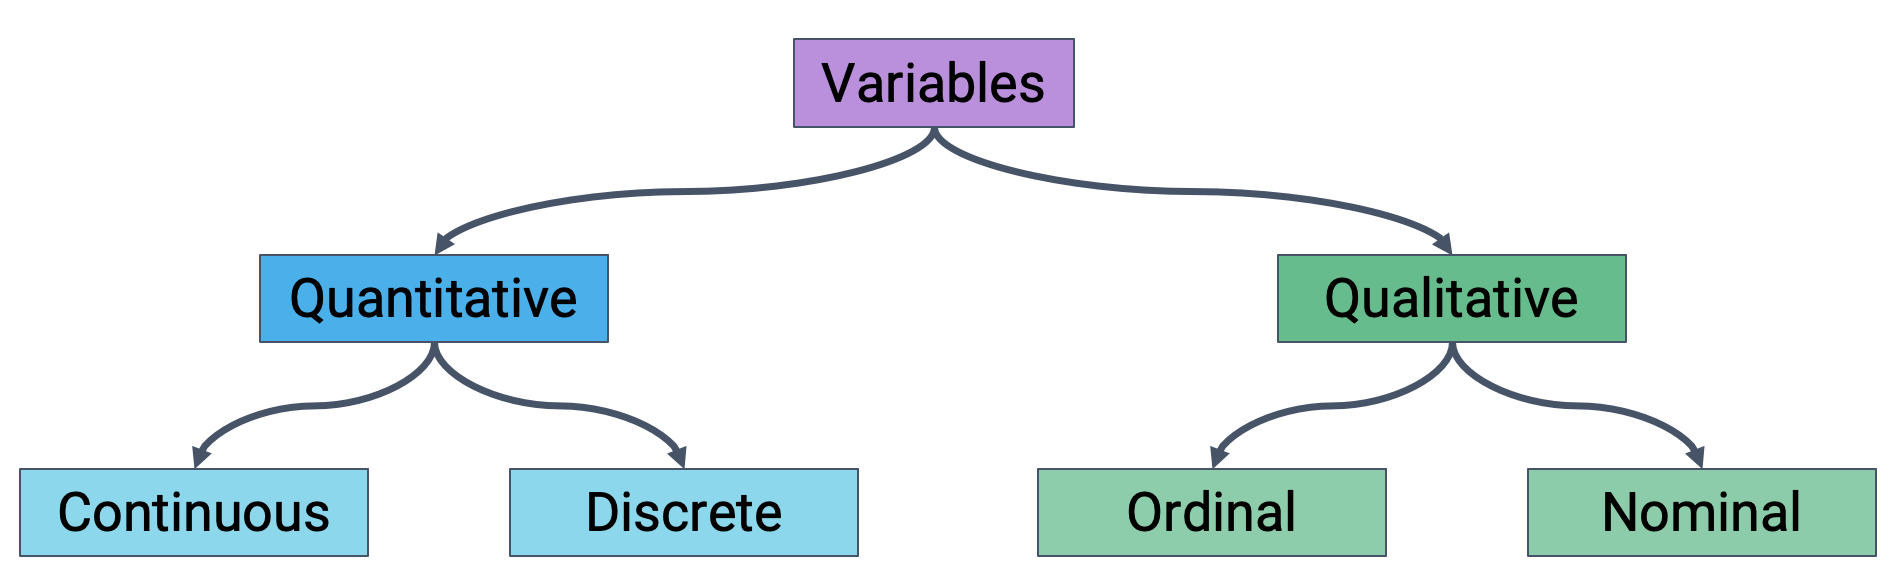
\includegraphics{eda/images/variable.png}

}

\caption{Classification of variable types}

\end{figure}%

Note that many variables don't sit neatly in just one of these
categories. Qualitative variables could have numeric levels, and
conversely, quantitative variables could be stored as strings.

\section{Granularity, Scope, and
Temporality}\label{granularity-scope-and-temporality}

After understanding the structure of the dataset, the next task is to
determine what exactly the data represents. We'll do so by considering
the data's granularity, scope, and temporality.

\subsection{Granularity}\label{granularity}

The \textbf{granularity} of a dataset is what a single row represents.
You can also think of it as the level of detail included in the data. To
determine the data's granularity, ask: what does each row in the dataset
represent? Fine-grained data contains a high level of detail, with a
single row representing a small individual unit. For example, each
record may represent one person. Coarse-grained data is encoded such
that a single row represents a large individual unit -- for example,
each record may represent a group of people.

\subsection{Scope}\label{scope}

The \textbf{scope} of a dataset is the subset of the population covered
by the data. If we were investigating student performance in Data
Science courses, a dataset with a narrow scope might encompass all
students enrolled in Data 100 whereas a dataset with an expansive scope
might encompass all students in California.

\subsection{Temporality}\label{temporality}

The \textbf{temporality} of a dataset describes the periodicity over
which the data was collected as well as when the data was most recently
collected or updated.

Time and date fields of a dataset could represent a few things:

\begin{enumerate}
\def\labelenumi{\arabic{enumi}.}
\tightlist
\item
  when the ``event'' happened
\item
  when the data was collected, or when it was entered into the system
\item
  when the data was copied into the database
\end{enumerate}

To fully understand the temporality of the data, it also may be
necessary to standardize time zones or inspect recurring time-based
trends in the data (do patterns recur in 24-hour periods? Over the
course of a month? Seasonally?). The convention for standardizing time
is the Coordinated Universal Time (UTC), an international time standard
measured at 0 degrees latitude that stays consistent throughout the year
(no daylight savings). We can represent Berkeley's time zone, Pacific
Standard Time (PST), as UTC-7 (with daylight savings).

\subsubsection{\texorpdfstring{Temporality with \texttt{pandas}'
\texttt{dt}
accessors}{Temporality with pandas' dt accessors}}\label{temporality-with-pandas-dt-accessors}

Let's briefly look at how we can use \texttt{pandas}' \texttt{dt}
accessors to work with dates/times in a dataset using the dataset you'll
see in Lab 3: the Berkeley PD Calls for Service dataset.

\begin{Shaded}
\begin{Highlighting}[]
\NormalTok{calls }\OperatorTok{=}\NormalTok{ pd.read\_csv(}\StringTok{"data/Berkeley\_PD\_{-}\_Calls\_for\_Service.csv"}\NormalTok{)}
\NormalTok{calls.head()}
\end{Highlighting}
\end{Shaded}

\begin{longtable}[]{@{}llllllllllll@{}}
\toprule\noalign{}
& CASENO & OFFENSE & EVENTDT & EVENTTM & CVLEGEND & CVDOW & InDbDate &
Block\_Location & BLKADDR & City & State \\
\midrule\noalign{}
\endhead
\bottomrule\noalign{}
\endlastfoot
0 & 21014296 & THEFT MISD. (UNDER \$950) & 04/01/2021 12:00:00 AM &
10:58 & LARCENY & 4 & 06/15/2021 12:00:00 AM & Berkeley,
CA\textbackslash r\textbackslash n(37.869058, -122.270455) & NaN &
Berkeley & CA \\
1 & 21014391 & THEFT MISD. (UNDER \$950) & 04/01/2021 12:00:00 AM &
10:38 & LARCENY & 4 & 06/15/2021 12:00:00 AM & Berkeley,
CA\textbackslash r\textbackslash n(37.869058, -122.270455) & NaN &
Berkeley & CA \\
2 & 21090494 & THEFT MISD. (UNDER \$950) & 04/19/2021 12:00:00 AM &
12:15 & LARCENY & 1 & 06/15/2021 12:00:00 AM & 2100 BLOCK HASTE
ST\textbackslash r\textbackslash nBerkeley,
CA\textbackslash r\textbackslash n(37.864... & 2100 BLOCK HASTE ST &
Berkeley & CA \\
3 & 21090204 & THEFT FELONY (OVER \$950) & 02/13/2021 12:00:00 AM &
17:00 & LARCENY & 6 & 06/15/2021 12:00:00 AM & 2600 BLOCK WARRING
ST\textbackslash r\textbackslash nBerkeley,
CA\textbackslash r\textbackslash n(37.8... & 2600 BLOCK WARRING ST &
Berkeley & CA \\
4 & 21090179 & BURGLARY AUTO & 02/08/2021 12:00:00 AM & 6:20 & BURGLARY
- VEHICLE & 1 & 06/15/2021 12:00:00 AM & 2700 BLOCK GARBER
ST\textbackslash r\textbackslash nBerkeley,
CA\textbackslash r\textbackslash n(37.86... & 2700 BLOCK GARBER ST &
Berkeley & CA \\
\end{longtable}

Looks like there are three columns with dates/times: \texttt{EVENTDT},
\texttt{EVENTTM}, and \texttt{InDbDate}.

Most likely, \texttt{EVENTDT} stands for the date when the event took
place, \texttt{EVENTTM} stands for the time of day the event took place
(in 24-hr format), and \texttt{InDbDate} is the date this call is
recorded onto the database.

If we check the data type of these columns, we will see they are stored
as strings. We can convert them to \texttt{datetime} objects using
pandas \texttt{to\_datetime} function.

\begin{Shaded}
\begin{Highlighting}[]
\NormalTok{calls[}\StringTok{"EVENTDT"}\NormalTok{] }\OperatorTok{=}\NormalTok{ pd.to\_datetime(calls[}\StringTok{"EVENTDT"}\NormalTok{])}
\NormalTok{calls.head()}
\end{Highlighting}
\end{Shaded}

\begin{verbatim}
C:\Users\yashd\AppData\Local\Temp\ipykernel_38392\874729699.py:1: UserWarning:

Could not infer format, so each element will be parsed individually, falling back to `dateutil`. To ensure parsing is consistent and as-expected, please specify a format.
\end{verbatim}

\begin{longtable}[]{@{}llllllllllll@{}}
\toprule\noalign{}
& CASENO & OFFENSE & EVENTDT & EVENTTM & CVLEGEND & CVDOW & InDbDate &
Block\_Location & BLKADDR & City & State \\
\midrule\noalign{}
\endhead
\bottomrule\noalign{}
\endlastfoot
0 & 21014296 & THEFT MISD. (UNDER \$950) & 2021-04-01 & 10:58 & LARCENY
& 4 & 06/15/2021 12:00:00 AM & Berkeley,
CA\textbackslash r\textbackslash n(37.869058, -122.270455) & NaN &
Berkeley & CA \\
1 & 21014391 & THEFT MISD. (UNDER \$950) & 2021-04-01 & 10:38 & LARCENY
& 4 & 06/15/2021 12:00:00 AM & Berkeley,
CA\textbackslash r\textbackslash n(37.869058, -122.270455) & NaN &
Berkeley & CA \\
2 & 21090494 & THEFT MISD. (UNDER \$950) & 2021-04-19 & 12:15 & LARCENY
& 1 & 06/15/2021 12:00:00 AM & 2100 BLOCK HASTE
ST\textbackslash r\textbackslash nBerkeley,
CA\textbackslash r\textbackslash n(37.864... & 2100 BLOCK HASTE ST &
Berkeley & CA \\
3 & 21090204 & THEFT FELONY (OVER \$950) & 2021-02-13 & 17:00 & LARCENY
& 6 & 06/15/2021 12:00:00 AM & 2600 BLOCK WARRING
ST\textbackslash r\textbackslash nBerkeley,
CA\textbackslash r\textbackslash n(37.8... & 2600 BLOCK WARRING ST &
Berkeley & CA \\
4 & 21090179 & BURGLARY AUTO & 2021-02-08 & 6:20 & BURGLARY - VEHICLE &
1 & 06/15/2021 12:00:00 AM & 2700 BLOCK GARBER
ST\textbackslash r\textbackslash nBerkeley,
CA\textbackslash r\textbackslash n(37.86... & 2700 BLOCK GARBER ST &
Berkeley & CA \\
\end{longtable}

Now, we can use the \texttt{dt} accessor on this column.

We can get the month:

\begin{Shaded}
\begin{Highlighting}[]
\NormalTok{calls[}\StringTok{"EVENTDT"}\NormalTok{].dt.month.head()}
\end{Highlighting}
\end{Shaded}

\begin{verbatim}
0    4
1    4
2    4
3    2
4    2
Name: EVENTDT, dtype: int32
\end{verbatim}

Which day of the week the date is on:

\begin{Shaded}
\begin{Highlighting}[]
\NormalTok{calls[}\StringTok{"EVENTDT"}\NormalTok{].dt.dayofweek.head()}
\end{Highlighting}
\end{Shaded}

\begin{verbatim}
0    3
1    3
2    0
3    5
4    0
Name: EVENTDT, dtype: int32
\end{verbatim}

Check the mimimum values to see if there are any suspicious-looking, 70s
dates:

\begin{Shaded}
\begin{Highlighting}[]
\NormalTok{calls.sort\_values(}\StringTok{"EVENTDT"}\NormalTok{).head()}
\end{Highlighting}
\end{Shaded}

\begin{longtable}[]{@{}llllllllllll@{}}
\toprule\noalign{}
& CASENO & OFFENSE & EVENTDT & EVENTTM & CVLEGEND & CVDOW & InDbDate &
Block\_Location & BLKADDR & City & State \\
\midrule\noalign{}
\endhead
\bottomrule\noalign{}
\endlastfoot
2513 & 20057398 & BURGLARY COMMERCIAL & 2020-12-17 & 16:05 & BURGLARY -
COMMERCIAL & 4 & 06/15/2021 12:00:00 AM & 600 BLOCK GILMAN
ST\textbackslash r\textbackslash nBerkeley,
CA\textbackslash r\textbackslash n(37.878... & 600 BLOCK GILMAN ST &
Berkeley & CA \\
624 & 20057207 & ASSAULT/BATTERY MISD. & 2020-12-17 & 16:50 & ASSAULT &
4 & 06/15/2021 12:00:00 AM & 2100 BLOCK SHATTUCK
AVE\textbackslash r\textbackslash nBerkeley,
CA\textbackslash r\textbackslash n(37... & 2100 BLOCK SHATTUCK AVE &
Berkeley & CA \\
154 & 20092214 & THEFT FROM AUTO & 2020-12-17 & 18:30 & LARCENY - FROM
VEHICLE & 4 & 06/15/2021 12:00:00 AM & 800 BLOCK SHATTUCK
AVE\textbackslash r\textbackslash nBerkeley,
CA\textbackslash r\textbackslash n(37.... & 800 BLOCK SHATTUCK AVE &
Berkeley & CA \\
659 & 20057324 & THEFT MISD. (UNDER \$950) & 2020-12-17 & 15:44 &
LARCENY & 4 & 06/15/2021 12:00:00 AM & 1800 BLOCK 4TH
ST\textbackslash r\textbackslash nBerkeley,
CA\textbackslash r\textbackslash n(37.86988... & 1800 BLOCK 4TH ST &
Berkeley & CA \\
993 & 20057573 & BURGLARY RESIDENTIAL & 2020-12-17 & 22:15 & BURGLARY -
RESIDENTIAL & 4 & 06/15/2021 12:00:00 AM & 1700 BLOCK STUART
ST\textbackslash r\textbackslash nBerkeley,
CA\textbackslash r\textbackslash n(37.85... & 1700 BLOCK STUART ST &
Berkeley & CA \\
\end{longtable}

Doesn't look like it! We are good!

We can also do many things with the \texttt{dt} accessor like switching
time zones and converting time back to UNIX/POSIX time. Check out the
documentation on
\href{https://pandas.pydata.org/docs/user_guide/basics.html\#basics-dt-accessors}{\texttt{.dt}
accessor} and
\href{https://pandas.pydata.org/docs/user_guide/timeseries.html\#}{time
series/date functionality}.

\section{Faithfulness}\label{faithfulness}

At this stage in our data cleaning and EDA workflow, we've achieved
quite a lot: we've identified how our data is structured, come to terms
with what information it encodes, and gained insight as to how it was
generated. Throughout this process, we should always recall the original
intent of our work in Data Science -- to use data to better understand
and model the real world. To achieve this goal, we need to ensure that
the data we use is faithful to reality; that is, that our data
accurately captures the ``real world.''

Data used in research or industry is often ``messy'' -- there may be
errors or inaccuracies that impact the faithfulness of the dataset.
Signs that data may not be faithful include:

\begin{itemize}
\tightlist
\item
  Unrealistic or ``incorrect'' values, such as negative counts,
  locations that don't exist, or dates set in the future
\item
  Violations of obvious dependencies, like an age that does not match a
  birthday
\item
  Clear signs that data was entered by hand, which can lead to spelling
  errors or fields that are incorrectly shifted
\item
  Signs of data falsification, such as fake email addresses or repeated
  use of the same names
\item
  Duplicated records or fields containing the same information
\item
  Truncated data, e.g.~Microsoft Excel would limit the number of rows to
  655536 and the number of columns to 255
\end{itemize}

We often solve some of these more common issues in the following ways:

\begin{itemize}
\tightlist
\item
  Spelling errors: apply corrections or drop records that aren't in a
  dictionary
\item
  Time zone inconsistencies: convert to a common time zone (e.g.~UTC)
\item
  Duplicated records or fields: identify and eliminate duplicates (using
  primary keys)
\item
  Unspecified or inconsistent units: infer the units and check that
  values are in reasonable ranges in the data
\end{itemize}

\subsection{Missing Values}\label{missing-values}

Another common issue encountered with real-world datasets is that of
missing data. One strategy to resolve this is to simply drop any records
with missing values from the dataset. This does, however, introduce the
risk of inducing biases -- it is possible that the missing or corrupt
records may be systemically related to some feature of interest in the
data. Another solution is to keep the data as \texttt{NaN} values.

A third method to address missing data is to perform
\textbf{imputation}: infer the missing values using other data available
in the dataset. There is a wide variety of imputation techniques that
can be implemented; some of the most common are listed below.

\begin{itemize}
\tightlist
\item
  Average imputation: replace missing values with the average value for
  that field
\item
  Hot deck imputation: replace missing values with some random value
\item
  Regression imputation: develop a model to predict missing values and
  replace with the predicted value from the model.
\item
  Multiple imputation: replace missing values with multiple random
  values
\end{itemize}

Regardless of the strategy used to deal with missing data, we should
think carefully about \emph{why} particular records or fields may be
missing -- this can help inform whether or not the absence of these
values is significant or meaningful.

\section{EDA Demo 1: Tuberculosis in the United
States}\label{eda-demo-1-tuberculosis-in-the-united-states}

Now, let's walk through the data-cleaning and EDA workflow to see what
can we learn about the presence of Tuberculosis in the United States!

We will examine the data included in the
\href{https://www.cdc.gov/mmwr/volumes/71/wr/mm7112a1.htm?s_cid=mm7112a1_w\#T1_down}{original
CDC article} published in 2021.

\subsection{CSVs and Field Names}\label{csvs-and-field-names}

Suppose Table 1 was saved as a CSV file located in
\texttt{data/cdc\_tuberculosis.csv}.

We can then explore the CSV (which is a text file, and does not contain
binary-encoded data) in many ways: 1. Using a text editor like emacs,
vim, VSCode, etc. 2. Opening the CSV directly in DataHub (read-only),
Excel, Google Sheets, etc. 3. The \texttt{Python} file object 4.
\texttt{pandas}, using \texttt{pd.read\_csv()}

To try out options 1 and 2, you can view or download the Tuberculosis
from the
\href{https://data100.datahub.berkeley.edu/hub/user-redirect/git-pull?repo=https\%3A\%2F\%2Fgithub.com\%2FDS-100\%2Ffa23-student&urlpath=lab\%2Ftree\%2Ffa23-student\%2Flecture\%2Flec05\%2Flec04-eda.ipynb&branch=main}{lecture
demo notebook} under the \texttt{data} folder in the left hand menu.
Notice how the CSV file is a type of \textbf{rectangular data (i.e.,
tabular data) stored as comma-separated values}.

Next, let's try out option 3 using the \texttt{Python} file object.
We'll look at the first four lines:

\begin{Shaded}
\begin{Highlighting}[]
\ControlFlowTok{with} \BuiltInTok{open}\NormalTok{(}\StringTok{"data/cdc\_tuberculosis.csv"}\NormalTok{, }\StringTok{"r"}\NormalTok{) }\ImportTok{as}\NormalTok{ f:}
\NormalTok{    i }\OperatorTok{=} \DecValTok{0}
    \ControlFlowTok{for}\NormalTok{ row }\KeywordTok{in}\NormalTok{ f:}
        \BuiltInTok{print}\NormalTok{(row)}
\NormalTok{        i }\OperatorTok{+=} \DecValTok{1}
        \ControlFlowTok{if}\NormalTok{ i }\OperatorTok{\textgreater{}} \DecValTok{3}\NormalTok{:}
            \ControlFlowTok{break}
\end{Highlighting}
\end{Shaded}

\begin{verbatim}
,No. of TB cases,,,TB incidence,,

U.S. jurisdiction,2019,2020,2021,2019,2020,2021

Total,"8,900","7,173","7,860",2.71,2.16,2.37

Alabama,87,72,92,1.77,1.43,1.83
\end{verbatim}

Whoa, why are there blank lines interspaced between the lines of the
CSV?

You may recall that all line breaks in text files are encoded as the
special newline character \texttt{\textbackslash{}n}. Python's
\texttt{print()} prints each string (including the newline), and an
additional newline on top of that.

If you're curious, we can use the \texttt{repr()} function to return the
raw string with all special characters:

\begin{Shaded}
\begin{Highlighting}[]
\ControlFlowTok{with} \BuiltInTok{open}\NormalTok{(}\StringTok{"data/cdc\_tuberculosis.csv"}\NormalTok{, }\StringTok{"r"}\NormalTok{) }\ImportTok{as}\NormalTok{ f:}
\NormalTok{    i }\OperatorTok{=} \DecValTok{0}
    \ControlFlowTok{for}\NormalTok{ row }\KeywordTok{in}\NormalTok{ f:}
        \BuiltInTok{print}\NormalTok{(}\BuiltInTok{repr}\NormalTok{(row)) }\CommentTok{\# print raw strings}
\NormalTok{        i }\OperatorTok{+=} \DecValTok{1}
        \ControlFlowTok{if}\NormalTok{ i }\OperatorTok{\textgreater{}} \DecValTok{3}\NormalTok{:}
            \ControlFlowTok{break}
\end{Highlighting}
\end{Shaded}

\begin{verbatim}
',No. of TB cases,,,TB incidence,,\n'
'U.S. jurisdiction,2019,2020,2021,2019,2020,2021\n'
'Total,"8,900","7,173","7,860",2.71,2.16,2.37\n'
'Alabama,87,72,92,1.77,1.43,1.83\n'
\end{verbatim}

Finally, let's try option 4 and use the tried-and-true Data 100
approach: \texttt{pandas}.

\begin{Shaded}
\begin{Highlighting}[]
\NormalTok{tb\_df }\OperatorTok{=}\NormalTok{ pd.read\_csv(}\StringTok{"data/cdc\_tuberculosis.csv"}\NormalTok{)}
\NormalTok{tb\_df.head()}
\end{Highlighting}
\end{Shaded}

\begin{longtable}[]{@{}llllllll@{}}
\toprule\noalign{}
& Unnamed: 0 & No. of TB cases & Unnamed: 2 & Unnamed: 3 & TB incidence
& Unnamed: 5 & Unnamed: 6 \\
\midrule\noalign{}
\endhead
\bottomrule\noalign{}
\endlastfoot
0 & U.S. jurisdiction & 2019 & 2020 & 2021 & 2019.00 & 2020.00 &
2021.00 \\
1 & Total & 8,900 & 7,173 & 7,860 & 2.71 & 2.16 & 2.37 \\
2 & Alabama & 87 & 72 & 92 & 1.77 & 1.43 & 1.83 \\
3 & Alaska & 58 & 58 & 58 & 7.91 & 7.92 & 7.92 \\
4 & Arizona & 183 & 136 & 129 & 2.51 & 1.89 & 1.77 \\
\end{longtable}

You may notice some strange things about this table: what's up with the
``Unnamed'' column names and the first row?

Congratulations --- you're ready to wrangle your data! Because of how
things are stored, we'll need to clean the data a bit to name our
columns better.

A reasonable first step is to identify the row with the right header.
The \texttt{pd.read\_csv()} function
(\href{https://pandas.pydata.org/docs/reference/api/pandas.read_csv.html}{documentation})
has the convenient \texttt{header} parameter that we can set to use the
elements in row 1 as the appropriate columns:

\begin{Shaded}
\begin{Highlighting}[]
\NormalTok{tb\_df }\OperatorTok{=}\NormalTok{ pd.read\_csv(}\StringTok{"data/cdc\_tuberculosis.csv"}\NormalTok{, header}\OperatorTok{=}\DecValTok{1}\NormalTok{) }\CommentTok{\# row index}
\NormalTok{tb\_df.head(}\DecValTok{5}\NormalTok{)}
\end{Highlighting}
\end{Shaded}

\begin{longtable}[]{@{}llllllll@{}}
\toprule\noalign{}
& U.S. jurisdiction & 2019 & 2020 & 2021 & 2019.1 & 2020.1 & 2021.1 \\
\midrule\noalign{}
\endhead
\bottomrule\noalign{}
\endlastfoot
0 & Total & 8,900 & 7,173 & 7,860 & 2.71 & 2.16 & 2.37 \\
1 & Alabama & 87 & 72 & 92 & 1.77 & 1.43 & 1.83 \\
2 & Alaska & 58 & 58 & 58 & 7.91 & 7.92 & 7.92 \\
3 & Arizona & 183 & 136 & 129 & 2.51 & 1.89 & 1.77 \\
4 & Arkansas & 64 & 59 & 69 & 2.12 & 1.96 & 2.28 \\
\end{longtable}

Wait\ldots but now we can't differentiate betwen the ``Number of TB
cases'' and ``TB incidence'' year columns. \texttt{pandas} has tried to
make our lives easier by automatically adding ``.1'' to the latter
columns, but this doesn't help us, as humans, understand the data.

We can do this manually with \texttt{df.rename()}
(\href{https://pandas.pydata.org/docs/reference/api/pandas.DataFrame.rename.html?highlight=rename\#pandas.DataFrame.rename}{documentation}):

\begin{Shaded}
\begin{Highlighting}[]
\NormalTok{rename\_dict }\OperatorTok{=}\NormalTok{ \{}\StringTok{\textquotesingle{}2019\textquotesingle{}}\NormalTok{: }\StringTok{\textquotesingle{}TB cases 2019\textquotesingle{}}\NormalTok{,}
               \StringTok{\textquotesingle{}2020\textquotesingle{}}\NormalTok{: }\StringTok{\textquotesingle{}TB cases 2020\textquotesingle{}}\NormalTok{,}
               \StringTok{\textquotesingle{}2021\textquotesingle{}}\NormalTok{: }\StringTok{\textquotesingle{}TB cases 2021\textquotesingle{}}\NormalTok{,}
               \StringTok{\textquotesingle{}2019.1\textquotesingle{}}\NormalTok{: }\StringTok{\textquotesingle{}TB incidence 2019\textquotesingle{}}\NormalTok{,}
               \StringTok{\textquotesingle{}2020.1\textquotesingle{}}\NormalTok{: }\StringTok{\textquotesingle{}TB incidence 2020\textquotesingle{}}\NormalTok{,}
               \StringTok{\textquotesingle{}2021.1\textquotesingle{}}\NormalTok{: }\StringTok{\textquotesingle{}TB incidence 2021\textquotesingle{}}\NormalTok{\}}
\NormalTok{tb\_df }\OperatorTok{=}\NormalTok{ tb\_df.rename(columns}\OperatorTok{=}\NormalTok{rename\_dict)}
\NormalTok{tb\_df.head(}\DecValTok{5}\NormalTok{)}
\end{Highlighting}
\end{Shaded}

\begin{longtable}[]{@{}llllllll@{}}
\toprule\noalign{}
& U.S. jurisdiction & TB cases 2019 & TB cases 2020 & TB cases 2021 & TB
incidence 2019 & TB incidence 2020 & TB incidence 2021 \\
\midrule\noalign{}
\endhead
\bottomrule\noalign{}
\endlastfoot
0 & Total & 8,900 & 7,173 & 7,860 & 2.71 & 2.16 & 2.37 \\
1 & Alabama & 87 & 72 & 92 & 1.77 & 1.43 & 1.83 \\
2 & Alaska & 58 & 58 & 58 & 7.91 & 7.92 & 7.92 \\
3 & Arizona & 183 & 136 & 129 & 2.51 & 1.89 & 1.77 \\
4 & Arkansas & 64 & 59 & 69 & 2.12 & 1.96 & 2.28 \\
\end{longtable}

\subsection{Record Granularity}\label{record-granularity}

You might already be wondering: what's up with that first record?

Row 0 is what we call a \textbf{rollup record}, or summary record. It's
often useful when displaying tables to humans. The \textbf{granularity}
of record 0 (Totals) vs the rest of the records (States) is different.

Okay, EDA step two. How was the rollup record aggregated?

Let's check if Total TB cases is the sum of all state TB cases. If we
sum over all rows, we should get \textbf{2x} the total cases in each of
our TB cases by year (why do you think this is?).

\begin{Shaded}
\begin{Highlighting}[]
\NormalTok{tb\_df.}\BuiltInTok{sum}\NormalTok{(axis}\OperatorTok{=}\DecValTok{0}\NormalTok{)}
\end{Highlighting}
\end{Shaded}

\begin{verbatim}
U.S. jurisdiction    TotalAlabamaAlaskaArizonaArkansasCaliforniaCol...
TB cases 2019        8,9008758183642,111666718245583029973261085237...
TB cases 2020        7,1737258136591,706525417194122219282169239376...
TB cases 2021        7,8609258129691,750585443194992281064255127494...
TB incidence 2019                                               109.94
TB incidence 2020                                                93.09
TB incidence 2021                                               102.94
dtype: object
\end{verbatim}

Whoa, what's going on with the TB cases in 2019, 2020, and 2021? Check
out the column types:

\begin{Shaded}
\begin{Highlighting}[]
\NormalTok{tb\_df.dtypes}
\end{Highlighting}
\end{Shaded}

\begin{verbatim}
U.S. jurisdiction     object
TB cases 2019         object
TB cases 2020         object
TB cases 2021         object
TB incidence 2019    float64
TB incidence 2020    float64
TB incidence 2021    float64
dtype: object
\end{verbatim}

Since there are commas in the values for TB cases, the numbers are read
as the \texttt{object} datatype, or \textbf{storage type} (close to the
\texttt{Python} string datatype), so \texttt{pandas} is concatenating
strings instead of adding integers (recall that Python can ``sum'', or
concatenate, strings together: \texttt{"data"\ +\ "100"} evaluates to
\texttt{"data100"}).

Fortunately \texttt{read\_csv} also has a \texttt{thousands} parameter
(\href{https://pandas.pydata.org/docs/reference/api/pandas.read_csv.html}{documentation}):

\begin{Shaded}
\begin{Highlighting}[]
\CommentTok{\# improve readability: chaining method calls with outer parentheses/line breaks}
\NormalTok{tb\_df }\OperatorTok{=}\NormalTok{ (}
\NormalTok{    pd.read\_csv(}\StringTok{"data/cdc\_tuberculosis.csv"}\NormalTok{, header}\OperatorTok{=}\DecValTok{1}\NormalTok{, thousands}\OperatorTok{=}\StringTok{\textquotesingle{},\textquotesingle{}}\NormalTok{)}
\NormalTok{    .rename(columns}\OperatorTok{=}\NormalTok{rename\_dict)}
\NormalTok{)}
\NormalTok{tb\_df.head(}\DecValTok{5}\NormalTok{)}
\end{Highlighting}
\end{Shaded}

\begin{longtable}[]{@{}llllllll@{}}
\toprule\noalign{}
& U.S. jurisdiction & TB cases 2019 & TB cases 2020 & TB cases 2021 & TB
incidence 2019 & TB incidence 2020 & TB incidence 2021 \\
\midrule\noalign{}
\endhead
\bottomrule\noalign{}
\endlastfoot
0 & Total & 8900 & 7173 & 7860 & 2.71 & 2.16 & 2.37 \\
1 & Alabama & 87 & 72 & 92 & 1.77 & 1.43 & 1.83 \\
2 & Alaska & 58 & 58 & 58 & 7.91 & 7.92 & 7.92 \\
3 & Arizona & 183 & 136 & 129 & 2.51 & 1.89 & 1.77 \\
4 & Arkansas & 64 & 59 & 69 & 2.12 & 1.96 & 2.28 \\
\end{longtable}

\begin{Shaded}
\begin{Highlighting}[]
\NormalTok{tb\_df.}\BuiltInTok{sum}\NormalTok{()}
\end{Highlighting}
\end{Shaded}

\begin{verbatim}
U.S. jurisdiction    TotalAlabamaAlaskaArizonaArkansasCaliforniaCol...
TB cases 2019                                                    17800
TB cases 2020                                                    14346
TB cases 2021                                                    15720
TB incidence 2019                                               109.94
TB incidence 2020                                                93.09
TB incidence 2021                                               102.94
dtype: object
\end{verbatim}

The total TB cases look right. Phew!

Let's just look at the records with \textbf{state-level granularity}:

\begin{Shaded}
\begin{Highlighting}[]
\NormalTok{state\_tb\_df }\OperatorTok{=}\NormalTok{ tb\_df[}\DecValTok{1}\NormalTok{:]}
\NormalTok{state\_tb\_df.head(}\DecValTok{5}\NormalTok{)}
\end{Highlighting}
\end{Shaded}

\begin{longtable}[]{@{}llllllll@{}}
\toprule\noalign{}
& U.S. jurisdiction & TB cases 2019 & TB cases 2020 & TB cases 2021 & TB
incidence 2019 & TB incidence 2020 & TB incidence 2021 \\
\midrule\noalign{}
\endhead
\bottomrule\noalign{}
\endlastfoot
1 & Alabama & 87 & 72 & 92 & 1.77 & 1.43 & 1.83 \\
2 & Alaska & 58 & 58 & 58 & 7.91 & 7.92 & 7.92 \\
3 & Arizona & 183 & 136 & 129 & 2.51 & 1.89 & 1.77 \\
4 & Arkansas & 64 & 59 & 69 & 2.12 & 1.96 & 2.28 \\
5 & California & 2111 & 1706 & 1750 & 5.35 & 4.32 & 4.46 \\
\end{longtable}

\subsection{Gather Census Data}\label{gather-census-data}

U.S. Census population estimates
\href{https://www.census.gov/data/tables/time-series/demo/popest/2010s-state-total.html}{source}
(2019),
\href{https://www.census.gov/data/tables/time-series/demo/popest/2020s-state-total.html}{source}
(2020-2021).

Running the below cells cleans the data. There are a few new methods
here: * \texttt{df.convert\_dtypes()}
(\href{https://pandas.pydata.org/docs/reference/api/pandas.DataFrame.convert_dtypes.html}{documentation})
conveniently converts all float dtypes into ints and is out of scope for
the class. * \texttt{df.drop\_na()}
(\href{https://pandas.pydata.org/docs/reference/api/pandas.DataFrame.dropna.html}{documentation})
will be explained in more detail next time.

\begin{Shaded}
\begin{Highlighting}[]
\CommentTok{\# 2010s census data}
\NormalTok{census\_2010s\_df }\OperatorTok{=}\NormalTok{ pd.read\_csv(}\StringTok{"data/nst{-}est2019{-}01.csv"}\NormalTok{, header}\OperatorTok{=}\DecValTok{3}\NormalTok{, thousands}\OperatorTok{=}\StringTok{","}\NormalTok{)}
\NormalTok{census\_2010s\_df }\OperatorTok{=}\NormalTok{ (}
\NormalTok{    census\_2010s\_df}
\NormalTok{    .reset\_index()}
\NormalTok{    .drop(columns}\OperatorTok{=}\NormalTok{[}\StringTok{"index"}\NormalTok{, }\StringTok{"Census"}\NormalTok{, }\StringTok{"Estimates Base"}\NormalTok{])}
\NormalTok{    .rename(columns}\OperatorTok{=}\NormalTok{\{}\StringTok{"Unnamed: 0"}\NormalTok{: }\StringTok{"Geographic Area"}\NormalTok{\})}
\NormalTok{    .convert\_dtypes()                 }\CommentTok{\# "smart" converting of columns, use at your own risk}
\NormalTok{    .dropna()                         }\CommentTok{\# we\textquotesingle{}ll introduce this next time}
\NormalTok{)}
\NormalTok{census\_2010s\_df[}\StringTok{\textquotesingle{}Geographic Area\textquotesingle{}}\NormalTok{] }\OperatorTok{=}\NormalTok{ census\_2010s\_df[}\StringTok{\textquotesingle{}Geographic Area\textquotesingle{}}\NormalTok{].}\BuiltInTok{str}\NormalTok{.strip(}\StringTok{\textquotesingle{}.\textquotesingle{}}\NormalTok{)}

\CommentTok{\# with pd.option\_context(\textquotesingle{}display.min\_rows\textquotesingle{}, 30): \# shows more rows}
\CommentTok{\#     display(census\_2010s\_df)}
    
\NormalTok{census\_2010s\_df.head(}\DecValTok{5}\NormalTok{)}
\end{Highlighting}
\end{Shaded}

\begin{longtable}[]{@{}llllllllllll@{}}
\toprule\noalign{}
& Geographic Area & 2010 & 2011 & 2012 & 2013 & 2014 & 2015 & 2016 &
2017 & 2018 & 2019 \\
\midrule\noalign{}
\endhead
\bottomrule\noalign{}
\endlastfoot
0 & United States & 309321666 & 311556874 & 313830990 & 315993715 &
318301008 & 320635163 & 322941311 & 324985539 & 326687501 & 328239523 \\
1 & Northeast & 55380134 & 55604223 & 55775216 & 55901806 & 56006011 &
56034684 & 56042330 & 56059240 & 56046620 & 55982803 \\
2 & Midwest & 66974416 & 67157800 & 67336743 & 67560379 & 67745167 &
67860583 & 67987540 & 68126781 & 68236628 & 68329004 \\
3 & South & 114866680 & 116006522 & 117241208 & 118364400 & 119624037 &
120997341 & 122351760 & 123542189 & 124569433 & 125580448 \\
4 & West & 72100436 & 72788329 & 73477823 & 74167130 & 74925793 &
75742555 & 76559681 & 77257329 & 77834820 & 78347268 \\
\end{longtable}

Occasionally, you will want to modify code that you have imported. To
reimport those modifications you can either use \texttt{python}'s
\texttt{importlib} library:

\begin{Shaded}
\begin{Highlighting}[]
\ImportTok{from}\NormalTok{ importlib }\ImportTok{import} \BuiltInTok{reload}
\BuiltInTok{reload}\NormalTok{(utils)}
\end{Highlighting}
\end{Shaded}

or use \texttt{iPython} magic which will intelligently import code when
files change:

\begin{Shaded}
\begin{Highlighting}[]
\OperatorTok{\%}\NormalTok{load\_ext autoreload}
\OperatorTok{\%}\NormalTok{autoreload }\DecValTok{2}
\end{Highlighting}
\end{Shaded}

\begin{Shaded}
\begin{Highlighting}[]
\CommentTok{\# census 2020s data}
\NormalTok{census\_2020s\_df }\OperatorTok{=}\NormalTok{ pd.read\_csv(}\StringTok{"data/NST{-}EST2022{-}POP.csv"}\NormalTok{, header}\OperatorTok{=}\DecValTok{3}\NormalTok{, thousands}\OperatorTok{=}\StringTok{","}\NormalTok{)}
\NormalTok{census\_2020s\_df }\OperatorTok{=}\NormalTok{ (}
\NormalTok{    census\_2020s\_df}
\NormalTok{    .reset\_index()}
\NormalTok{    .drop(columns}\OperatorTok{=}\NormalTok{[}\StringTok{"index"}\NormalTok{, }\StringTok{"Unnamed: 1"}\NormalTok{])}
\NormalTok{    .rename(columns}\OperatorTok{=}\NormalTok{\{}\StringTok{"Unnamed: 0"}\NormalTok{: }\StringTok{"Geographic Area"}\NormalTok{\})}
\NormalTok{    .convert\_dtypes()                 }\CommentTok{\# "smart" converting of columns, use at your own risk}
\NormalTok{    .dropna()                         }\CommentTok{\# we\textquotesingle{}ll introduce this next time}
\NormalTok{)}
\NormalTok{census\_2020s\_df[}\StringTok{\textquotesingle{}Geographic Area\textquotesingle{}}\NormalTok{] }\OperatorTok{=}\NormalTok{ census\_2020s\_df[}\StringTok{\textquotesingle{}Geographic Area\textquotesingle{}}\NormalTok{].}\BuiltInTok{str}\NormalTok{.strip(}\StringTok{\textquotesingle{}.\textquotesingle{}}\NormalTok{)}

\NormalTok{census\_2020s\_df.head(}\DecValTok{5}\NormalTok{)}
\end{Highlighting}
\end{Shaded}

\begin{longtable}[]{@{}lllll@{}}
\toprule\noalign{}
& Geographic Area & 2020 & 2021 & 2022 \\
\midrule\noalign{}
\endhead
\bottomrule\noalign{}
\endlastfoot
0 & United States & 331511512 & 332031554 & 333287557 \\
1 & Northeast & 57448898 & 57259257 & 57040406 \\
2 & Midwest & 68961043 & 68836505 & 68787595 \\
3 & South & 126450613 & 127346029 & 128716192 \\
4 & West & 78650958 & 78589763 & 78743364 \\
\end{longtable}

\subsection{\texorpdfstring{Joining Data (Merging
\texttt{DataFrame}s)}{Joining Data (Merging DataFrames)}}\label{joining-data-merging-dataframes}

Time to \texttt{merge}! Here we use the \texttt{DataFrame} method
\texttt{df1.merge(right=df2,\ ...)} on \texttt{DataFrame} \texttt{df1}
(\href{https://pandas.pydata.org/docs/reference/api/pandas.DataFrame.merge.html}{documentation}).
Contrast this with the function
\texttt{pd.merge(left=df1,\ right=df2,\ ...)}
(\href{https://pandas.pydata.org/docs/reference/api/pandas.merge.html?highlight=pandas\%20merge\#pandas.merge}{documentation}).
Feel free to use either.

\begin{Shaded}
\begin{Highlighting}[]
\CommentTok{\# merge TB DataFrame with two US census DataFrames}
\NormalTok{tb\_census\_df }\OperatorTok{=}\NormalTok{ (}
\NormalTok{    tb\_df}
\NormalTok{    .merge(right}\OperatorTok{=}\NormalTok{census\_2010s\_df,}
\NormalTok{           left\_on}\OperatorTok{=}\StringTok{"U.S. jurisdiction"}\NormalTok{, right\_on}\OperatorTok{=}\StringTok{"Geographic Area"}\NormalTok{)}
\NormalTok{    .merge(right}\OperatorTok{=}\NormalTok{census\_2020s\_df,}
\NormalTok{           left\_on}\OperatorTok{=}\StringTok{"U.S. jurisdiction"}\NormalTok{, right\_on}\OperatorTok{=}\StringTok{"Geographic Area"}\NormalTok{)}
\NormalTok{)}
\NormalTok{tb\_census\_df.head(}\DecValTok{5}\NormalTok{)}
\end{Highlighting}
\end{Shaded}

\begin{longtable}[]{@{}lllllllllllllllllllllll@{}}
\toprule\noalign{}
& U.S. jurisdiction & TB cases 2019 & TB cases 2020 & TB cases 2021 & TB
incidence 2019 & TB incidence 2020 & TB incidence 2021 & Geographic
Area\_x & 2010 & 2011 & 2012 & 2013 & 2014 & 2015 & 2016 & 2017 & 2018 &
2019 & Geographic Area\_y & 2020 & 2021 & 2022 \\
\midrule\noalign{}
\endhead
\bottomrule\noalign{}
\endlastfoot
0 & Alabama & 87 & 72 & 92 & 1.77 & 1.43 & 1.83 & Alabama & 4785437 &
4799069 & 4815588 & 4830081 & 4841799 & 4852347 & 4863525 & 4874486 &
4887681 & 4903185 & Alabama & 5031362 & 5049846 & 5074296 \\
1 & Alaska & 58 & 58 & 58 & 7.91 & 7.92 & 7.92 & Alaska & 713910 &
722128 & 730443 & 737068 & 736283 & 737498 & 741456 & 739700 & 735139 &
731545 & Alaska & 732923 & 734182 & 733583 \\
2 & Arizona & 183 & 136 & 129 & 2.51 & 1.89 & 1.77 & Arizona & 6407172 &
6472643 & 6554978 & 6632764 & 6730413 & 6829676 & 6941072 & 7044008 &
7158024 & 7278717 & Arizona & 7179943 & 7264877 & 7359197 \\
3 & Arkansas & 64 & 59 & 69 & 2.12 & 1.96 & 2.28 & Arkansas & 2921964 &
2940667 & 2952164 & 2959400 & 2967392 & 2978048 & 2989918 & 3001345 &
3009733 & 3017804 & Arkansas & 3014195 & 3028122 & 3045637 \\
4 & California & 2111 & 1706 & 1750 & 5.35 & 4.32 & 4.46 & California &
37319502 & 37638369 & 37948800 & 38260787 & 38596972 & 38918045 &
39167117 & 39358497 & 39461588 & 39512223 & California & 39501653 &
39142991 & 39029342 \\
\end{longtable}

Having all of these columns is a little unwieldy. We could either drop
the unneeded columns now, or just merge on smaller census
\texttt{DataFrame}s. Let's do the latter.

\begin{Shaded}
\begin{Highlighting}[]
\CommentTok{\# try merging again, but cleaner this time}
\NormalTok{tb\_census\_df }\OperatorTok{=}\NormalTok{ (}
\NormalTok{    tb\_df}
\NormalTok{    .merge(right}\OperatorTok{=}\NormalTok{census\_2010s\_df[[}\StringTok{"Geographic Area"}\NormalTok{, }\StringTok{"2019"}\NormalTok{]],}
\NormalTok{           left\_on}\OperatorTok{=}\StringTok{"U.S. jurisdiction"}\NormalTok{, right\_on}\OperatorTok{=}\StringTok{"Geographic Area"}\NormalTok{)}
\NormalTok{    .drop(columns}\OperatorTok{=}\StringTok{"Geographic Area"}\NormalTok{)}
\NormalTok{    .merge(right}\OperatorTok{=}\NormalTok{census\_2020s\_df[[}\StringTok{"Geographic Area"}\NormalTok{, }\StringTok{"2020"}\NormalTok{, }\StringTok{"2021"}\NormalTok{]],}
\NormalTok{           left\_on}\OperatorTok{=}\StringTok{"U.S. jurisdiction"}\NormalTok{, right\_on}\OperatorTok{=}\StringTok{"Geographic Area"}\NormalTok{)}
\NormalTok{    .drop(columns}\OperatorTok{=}\StringTok{"Geographic Area"}\NormalTok{)}
\NormalTok{)}
\NormalTok{tb\_census\_df.head(}\DecValTok{5}\NormalTok{)}
\end{Highlighting}
\end{Shaded}

\begin{longtable}[]{@{}lllllllllll@{}}
\toprule\noalign{}
& U.S. jurisdiction & TB cases 2019 & TB cases 2020 & TB cases 2021 & TB
incidence 2019 & TB incidence 2020 & TB incidence 2021 & 2019 & 2020 &
2021 \\
\midrule\noalign{}
\endhead
\bottomrule\noalign{}
\endlastfoot
0 & Alabama & 87 & 72 & 92 & 1.77 & 1.43 & 1.83 & 4903185 & 5031362 &
5049846 \\
1 & Alaska & 58 & 58 & 58 & 7.91 & 7.92 & 7.92 & 731545 & 732923 &
734182 \\
2 & Arizona & 183 & 136 & 129 & 2.51 & 1.89 & 1.77 & 7278717 & 7179943 &
7264877 \\
3 & Arkansas & 64 & 59 & 69 & 2.12 & 1.96 & 2.28 & 3017804 & 3014195 &
3028122 \\
4 & California & 2111 & 1706 & 1750 & 5.35 & 4.32 & 4.46 & 39512223 &
39501653 & 39142991 \\
\end{longtable}

\subsection{Reproducing Data: Compute
Incidence}\label{reproducing-data-compute-incidence}

Let's recompute incidence to make sure we know where the original CDC
numbers came from.

From the
\href{https://www.cdc.gov/mmwr/volumes/71/wr/mm7112a1.htm?s_cid=mm7112a1_w\#T1_down}{CDC
report}: TB incidence is computed as ``Cases per 100,000 persons using
mid-year population estimates from the U.S. Census Bureau.''

If we define a group as 100,000 people, then we can compute the TB
incidence for a given state population as

\[\text{TB incidence} = \frac{\text{TB cases in population}}{\text{groups in population}} = \frac{\text{TB cases in population}}{\text{population}/100000} \]

\[= \frac{\text{TB cases in population}}{\text{population}} \times 100000\]

Let's try this for 2019:

\begin{Shaded}
\begin{Highlighting}[]
\NormalTok{tb\_census\_df[}\StringTok{"recompute incidence 2019"}\NormalTok{] }\OperatorTok{=}\NormalTok{ tb\_census\_df[}\StringTok{"TB cases 2019"}\NormalTok{]}\OperatorTok{/}\NormalTok{tb\_census\_df[}\StringTok{"2019"}\NormalTok{]}\OperatorTok{*}\DecValTok{100000}
\NormalTok{tb\_census\_df.head(}\DecValTok{5}\NormalTok{)}
\end{Highlighting}
\end{Shaded}

\begin{longtable}[]{@{}llllllllllll@{}}
\toprule\noalign{}
& U.S. jurisdiction & TB cases 2019 & TB cases 2020 & TB cases 2021 & TB
incidence 2019 & TB incidence 2020 & TB incidence 2021 & 2019 & 2020 &
2021 & recompute incidence 2019 \\
\midrule\noalign{}
\endhead
\bottomrule\noalign{}
\endlastfoot
0 & Alabama & 87 & 72 & 92 & 1.77 & 1.43 & 1.83 & 4903185 & 5031362 &
5049846 & 1.77 \\
1 & Alaska & 58 & 58 & 58 & 7.91 & 7.92 & 7.92 & 731545 & 732923 &
734182 & 7.93 \\
2 & Arizona & 183 & 136 & 129 & 2.51 & 1.89 & 1.77 & 7278717 & 7179943 &
7264877 & 2.51 \\
3 & Arkansas & 64 & 59 & 69 & 2.12 & 1.96 & 2.28 & 3017804 & 3014195 &
3028122 & 2.12 \\
4 & California & 2111 & 1706 & 1750 & 5.35 & 4.32 & 4.46 & 39512223 &
39501653 & 39142991 & 5.34 \\
\end{longtable}

Awesome!!!

Let's use a for-loop and Python format strings to compute TB incidence
for all years. Python f-strings are just used for the purposes of this
demo, but they're handy to know when you explore data beyond this course
(\href{https://docs.python.org/3/tutorial/inputoutput.html}{documentation}).

\begin{Shaded}
\begin{Highlighting}[]
\CommentTok{\# recompute incidence for all years}
\ControlFlowTok{for}\NormalTok{ year }\KeywordTok{in}\NormalTok{ [}\DecValTok{2019}\NormalTok{, }\DecValTok{2020}\NormalTok{, }\DecValTok{2021}\NormalTok{]:}
\NormalTok{    tb\_census\_df[}\SpecialStringTok{f"recompute incidence }\SpecialCharTok{\{}\NormalTok{year}\SpecialCharTok{\}}\SpecialStringTok{"}\NormalTok{] }\OperatorTok{=}\NormalTok{ tb\_census\_df[}\SpecialStringTok{f"TB cases }\SpecialCharTok{\{}\NormalTok{year}\SpecialCharTok{\}}\SpecialStringTok{"}\NormalTok{]}\OperatorTok{/}\NormalTok{tb\_census\_df[}\SpecialStringTok{f"}\SpecialCharTok{\{}\NormalTok{year}\SpecialCharTok{\}}\SpecialStringTok{"}\NormalTok{]}\OperatorTok{*}\DecValTok{100000}
\NormalTok{tb\_census\_df.head(}\DecValTok{5}\NormalTok{)}
\end{Highlighting}
\end{Shaded}

\begin{longtable}[]{@{}llllllllllllll@{}}
\toprule\noalign{}
& U.S. jurisdiction & TB cases 2019 & TB cases 2020 & TB cases 2021 & TB
incidence 2019 & TB incidence 2020 & TB incidence 2021 & 2019 & 2020 &
2021 & recompute incidence 2019 & recompute incidence 2020 & recompute
incidence 2021 \\
\midrule\noalign{}
\endhead
\bottomrule\noalign{}
\endlastfoot
0 & Alabama & 87 & 72 & 92 & 1.77 & 1.43 & 1.83 & 4903185 & 5031362 &
5049846 & 1.77 & 1.43 & 1.82 \\
1 & Alaska & 58 & 58 & 58 & 7.91 & 7.92 & 7.92 & 731545 & 732923 &
734182 & 7.93 & 7.91 & 7.90 \\
2 & Arizona & 183 & 136 & 129 & 2.51 & 1.89 & 1.77 & 7278717 & 7179943 &
7264877 & 2.51 & 1.89 & 1.78 \\
3 & Arkansas & 64 & 59 & 69 & 2.12 & 1.96 & 2.28 & 3017804 & 3014195 &
3028122 & 2.12 & 1.96 & 2.28 \\
4 & California & 2111 & 1706 & 1750 & 5.35 & 4.32 & 4.46 & 39512223 &
39501653 & 39142991 & 5.34 & 4.32 & 4.47 \\
\end{longtable}

These numbers look pretty close!!! There are a few errors in the
hundredths place, particularly in 2021. It may be useful to further
explore reasons behind this discrepancy.

\begin{Shaded}
\begin{Highlighting}[]
\NormalTok{tb\_census\_df.describe()}
\end{Highlighting}
\end{Shaded}

\begin{longtable}[]{@{}lllllllllllll@{}}
\toprule\noalign{}
& TB cases 2019 & TB cases 2020 & TB cases 2021 & TB incidence 2019 & TB
incidence 2020 & TB incidence 2021 & 2019 & 2020 & 2021 & recompute
incidence 2019 & recompute incidence 2020 & recompute incidence 2021 \\
\midrule\noalign{}
\endhead
\bottomrule\noalign{}
\endlastfoot
count & 51.00 & 51.00 & 51.00 & 51.00 & 51.00 & 51.00 & 51.00 & 51.00 &
51.00 & 51.00 & 51.00 & 51.00 \\
mean & 174.51 & 140.65 & 154.12 & 2.10 & 1.78 & 1.97 & 6436069.08 &
6500225.73 & 6510422.63 & 2.10 & 1.78 & 1.97 \\
std & 341.74 & 271.06 & 286.78 & 1.50 & 1.34 & 1.48 & 7360660.47 &
7408168.46 & 7394300.08 & 1.50 & 1.34 & 1.47 \\
min & 1.00 & 0.00 & 2.00 & 0.17 & 0.00 & 0.21 & 578759.00 & 577605.00 &
579483.00 & 0.17 & 0.00 & 0.21 \\
25\% & 25.50 & 29.00 & 23.00 & 1.29 & 1.21 & 1.23 & 1789606.00 &
1820311.00 & 1844920.00 & 1.30 & 1.21 & 1.23 \\
50\% & 70.00 & 67.00 & 69.00 & 1.80 & 1.52 & 1.70 & 4467673.00 &
4507445.00 & 4506589.00 & 1.81 & 1.52 & 1.69 \\
75\% & 180.50 & 139.00 & 150.00 & 2.58 & 1.99 & 2.22 & 7446805.00 &
7451987.00 & 7502811.00 & 2.58 & 1.99 & 2.22 \\
max & 2111.00 & 1706.00 & 1750.00 & 7.91 & 7.92 & 7.92 & 39512223.00 &
39501653.00 & 39142991.00 & 7.93 & 7.91 & 7.90 \\
\end{longtable}

\subsection{Bonus EDA: Reproducing the Reported
Statistic}\label{bonus-eda-reproducing-the-reported-statistic}

\textbf{How do we reproduce that reported statistic in the original
\href{https://www.cdc.gov/mmwr/volumes/71/wr/mm7112a1.htm?s_cid=mm7112a1_w}{CDC
report}?}

\begin{quote}
Reported TB incidence (cases per 100,000 persons) increased
\textbf{9.4\%}, from \textbf{2.2} during 2020 to \textbf{2.4} during
2021 but was lower than incidence during 2019 (2.7). Increases occurred
among both U.S.-born and non--U.S.-born persons.
\end{quote}

This is TB incidence computed across the entire U.S. population! How do
we reproduce this? * We need to reproduce the ``Total'' TB incidences in
our rolled record. * But our current \texttt{tb\_census\_df} only has 51
entries (50 states plus Washington, D.C.). There is no rolled record. *
What happened\ldots?

Let's get exploring!

Before we keep exploring, we'll set all indexes to more meaningful
values, instead of just numbers that pertain to some row at some point.
This will make our cleaning slightly easier.

\begin{Shaded}
\begin{Highlighting}[]
\NormalTok{tb\_df }\OperatorTok{=}\NormalTok{ tb\_df.set\_index(}\StringTok{"U.S. jurisdiction"}\NormalTok{)}
\NormalTok{tb\_df.head(}\DecValTok{5}\NormalTok{)}
\end{Highlighting}
\end{Shaded}

\begin{longtable}[]{@{}lllllll@{}}
\toprule\noalign{}
& TB cases 2019 & TB cases 2020 & TB cases 2021 & TB incidence 2019 & TB
incidence 2020 & TB incidence 2021 \\
U.S. jurisdiction & & & & & & \\
\midrule\noalign{}
\endhead
\bottomrule\noalign{}
\endlastfoot
Total & 8900 & 7173 & 7860 & 2.71 & 2.16 & 2.37 \\
Alabama & 87 & 72 & 92 & 1.77 & 1.43 & 1.83 \\
Alaska & 58 & 58 & 58 & 7.91 & 7.92 & 7.92 \\
Arizona & 183 & 136 & 129 & 2.51 & 1.89 & 1.77 \\
Arkansas & 64 & 59 & 69 & 2.12 & 1.96 & 2.28 \\
\end{longtable}

\begin{Shaded}
\begin{Highlighting}[]
\NormalTok{census\_2010s\_df }\OperatorTok{=}\NormalTok{ census\_2010s\_df.set\_index(}\StringTok{"Geographic Area"}\NormalTok{)}
\NormalTok{census\_2010s\_df.head(}\DecValTok{5}\NormalTok{)}
\end{Highlighting}
\end{Shaded}

\begin{longtable}[]{@{}lllllllllll@{}}
\toprule\noalign{}
& 2010 & 2011 & 2012 & 2013 & 2014 & 2015 & 2016 & 2017 & 2018 & 2019 \\
Geographic Area & & & & & & & & & & \\
\midrule\noalign{}
\endhead
\bottomrule\noalign{}
\endlastfoot
United States & 309321666 & 311556874 & 313830990 & 315993715 &
318301008 & 320635163 & 322941311 & 324985539 & 326687501 & 328239523 \\
Northeast & 55380134 & 55604223 & 55775216 & 55901806 & 56006011 &
56034684 & 56042330 & 56059240 & 56046620 & 55982803 \\
Midwest & 66974416 & 67157800 & 67336743 & 67560379 & 67745167 &
67860583 & 67987540 & 68126781 & 68236628 & 68329004 \\
South & 114866680 & 116006522 & 117241208 & 118364400 & 119624037 &
120997341 & 122351760 & 123542189 & 124569433 & 125580448 \\
West & 72100436 & 72788329 & 73477823 & 74167130 & 74925793 & 75742555 &
76559681 & 77257329 & 77834820 & 78347268 \\
\end{longtable}

\begin{Shaded}
\begin{Highlighting}[]
\NormalTok{census\_2020s\_df }\OperatorTok{=}\NormalTok{ census\_2020s\_df.set\_index(}\StringTok{"Geographic Area"}\NormalTok{)}
\NormalTok{census\_2020s\_df.head(}\DecValTok{5}\NormalTok{)}
\end{Highlighting}
\end{Shaded}

\begin{longtable}[]{@{}llll@{}}
\toprule\noalign{}
& 2020 & 2021 & 2022 \\
Geographic Area & & & \\
\midrule\noalign{}
\endhead
\bottomrule\noalign{}
\endlastfoot
United States & 331511512 & 332031554 & 333287557 \\
Northeast & 57448898 & 57259257 & 57040406 \\
Midwest & 68961043 & 68836505 & 68787595 \\
South & 126450613 & 127346029 & 128716192 \\
West & 78650958 & 78589763 & 78743364 \\
\end{longtable}

It turns out that our merge above only kept state records, even though
our original \texttt{tb\_df} had the ``Total'' rolled record:

\begin{Shaded}
\begin{Highlighting}[]
\NormalTok{tb\_df.head()}
\end{Highlighting}
\end{Shaded}

\begin{longtable}[]{@{}lllllll@{}}
\toprule\noalign{}
& TB cases 2019 & TB cases 2020 & TB cases 2021 & TB incidence 2019 & TB
incidence 2020 & TB incidence 2021 \\
U.S. jurisdiction & & & & & & \\
\midrule\noalign{}
\endhead
\bottomrule\noalign{}
\endlastfoot
Total & 8900 & 7173 & 7860 & 2.71 & 2.16 & 2.37 \\
Alabama & 87 & 72 & 92 & 1.77 & 1.43 & 1.83 \\
Alaska & 58 & 58 & 58 & 7.91 & 7.92 & 7.92 \\
Arizona & 183 & 136 & 129 & 2.51 & 1.89 & 1.77 \\
Arkansas & 64 & 59 & 69 & 2.12 & 1.96 & 2.28 \\
\end{longtable}

Recall that \texttt{merge} by default does an \textbf{inner} merge by
default, meaning that it only preserves keys that are present in
\textbf{both} \texttt{DataFrame}s.

The rolled records in our census \texttt{DataFrame} have different
\texttt{Geographic\ Area} fields, which was the key we merged on:

\begin{Shaded}
\begin{Highlighting}[]
\NormalTok{census\_2010s\_df.head(}\DecValTok{5}\NormalTok{)}
\end{Highlighting}
\end{Shaded}

\begin{longtable}[]{@{}lllllllllll@{}}
\toprule\noalign{}
& 2010 & 2011 & 2012 & 2013 & 2014 & 2015 & 2016 & 2017 & 2018 & 2019 \\
Geographic Area & & & & & & & & & & \\
\midrule\noalign{}
\endhead
\bottomrule\noalign{}
\endlastfoot
United States & 309321666 & 311556874 & 313830990 & 315993715 &
318301008 & 320635163 & 322941311 & 324985539 & 326687501 & 328239523 \\
Northeast & 55380134 & 55604223 & 55775216 & 55901806 & 56006011 &
56034684 & 56042330 & 56059240 & 56046620 & 55982803 \\
Midwest & 66974416 & 67157800 & 67336743 & 67560379 & 67745167 &
67860583 & 67987540 & 68126781 & 68236628 & 68329004 \\
South & 114866680 & 116006522 & 117241208 & 118364400 & 119624037 &
120997341 & 122351760 & 123542189 & 124569433 & 125580448 \\
West & 72100436 & 72788329 & 73477823 & 74167130 & 74925793 & 75742555 &
76559681 & 77257329 & 77834820 & 78347268 \\
\end{longtable}

The Census \texttt{DataFrame} has several rolled records. The aggregate
record we are looking for actually has the Geographic Area named
``United States''.

One straightforward way to get the right merge is to rename the value
itself. Because we now have the Geographic Area index, we'll use
\texttt{df.rename()}
(\href{https://pandas.pydata.org/docs/reference/api/pandas.DataFrame.rename.html}{documentation}):

\begin{Shaded}
\begin{Highlighting}[]
\CommentTok{\# rename rolled record for 2010s}
\NormalTok{census\_2010s\_df.rename(index}\OperatorTok{=}\NormalTok{\{}\StringTok{\textquotesingle{}United States\textquotesingle{}}\NormalTok{:}\StringTok{\textquotesingle{}Total\textquotesingle{}}\NormalTok{\}, inplace}\OperatorTok{=}\VariableTok{True}\NormalTok{)}
\NormalTok{census\_2010s\_df.head(}\DecValTok{5}\NormalTok{)}
\end{Highlighting}
\end{Shaded}

\begin{longtable}[]{@{}lllllllllll@{}}
\toprule\noalign{}
& 2010 & 2011 & 2012 & 2013 & 2014 & 2015 & 2016 & 2017 & 2018 & 2019 \\
Geographic Area & & & & & & & & & & \\
\midrule\noalign{}
\endhead
\bottomrule\noalign{}
\endlastfoot
Total & 309321666 & 311556874 & 313830990 & 315993715 & 318301008 &
320635163 & 322941311 & 324985539 & 326687501 & 328239523 \\
Northeast & 55380134 & 55604223 & 55775216 & 55901806 & 56006011 &
56034684 & 56042330 & 56059240 & 56046620 & 55982803 \\
Midwest & 66974416 & 67157800 & 67336743 & 67560379 & 67745167 &
67860583 & 67987540 & 68126781 & 68236628 & 68329004 \\
South & 114866680 & 116006522 & 117241208 & 118364400 & 119624037 &
120997341 & 122351760 & 123542189 & 124569433 & 125580448 \\
West & 72100436 & 72788329 & 73477823 & 74167130 & 74925793 & 75742555 &
76559681 & 77257329 & 77834820 & 78347268 \\
\end{longtable}

\begin{Shaded}
\begin{Highlighting}[]
\CommentTok{\# same, but for 2020s rename rolled record}
\NormalTok{census\_2020s\_df.rename(index}\OperatorTok{=}\NormalTok{\{}\StringTok{\textquotesingle{}United States\textquotesingle{}}\NormalTok{:}\StringTok{\textquotesingle{}Total\textquotesingle{}}\NormalTok{\}, inplace}\OperatorTok{=}\VariableTok{True}\NormalTok{)}
\NormalTok{census\_2020s\_df.head(}\DecValTok{5}\NormalTok{)}
\end{Highlighting}
\end{Shaded}

\begin{longtable}[]{@{}llll@{}}
\toprule\noalign{}
& 2020 & 2021 & 2022 \\
Geographic Area & & & \\
\midrule\noalign{}
\endhead
\bottomrule\noalign{}
\endlastfoot
Total & 331511512 & 332031554 & 333287557 \\
Northeast & 57448898 & 57259257 & 57040406 \\
Midwest & 68961043 & 68836505 & 68787595 \\
South & 126450613 & 127346029 & 128716192 \\
West & 78650958 & 78589763 & 78743364 \\
\end{longtable}

Next let's rerun our merge. Note the different chaining, because we are
now merging on indexes (\texttt{df.merge()}
\href{https://pandas.pydata.org/docs/reference/api/pandas.DataFrame.merge.html}{documentation}).

\begin{Shaded}
\begin{Highlighting}[]
\NormalTok{tb\_census\_df }\OperatorTok{=}\NormalTok{ (}
\NormalTok{    tb\_df}
\NormalTok{    .merge(right}\OperatorTok{=}\NormalTok{census\_2010s\_df[[}\StringTok{"2019"}\NormalTok{]],}
\NormalTok{           left\_index}\OperatorTok{=}\VariableTok{True}\NormalTok{, right\_index}\OperatorTok{=}\VariableTok{True}\NormalTok{)}
\NormalTok{    .merge(right}\OperatorTok{=}\NormalTok{census\_2020s\_df[[}\StringTok{"2020"}\NormalTok{, }\StringTok{"2021"}\NormalTok{]],}
\NormalTok{           left\_index}\OperatorTok{=}\VariableTok{True}\NormalTok{, right\_index}\OperatorTok{=}\VariableTok{True}\NormalTok{)}
\NormalTok{)}
\NormalTok{tb\_census\_df.head(}\DecValTok{5}\NormalTok{)}
\end{Highlighting}
\end{Shaded}

\begin{longtable}[]{@{}llllllllll@{}}
\toprule\noalign{}
& TB cases 2019 & TB cases 2020 & TB cases 2021 & TB incidence 2019 & TB
incidence 2020 & TB incidence 2021 & 2019 & 2020 & 2021 \\
\midrule\noalign{}
\endhead
\bottomrule\noalign{}
\endlastfoot
Total & 8900 & 7173 & 7860 & 2.71 & 2.16 & 2.37 & 328239523 & 331511512
& 332031554 \\
Alabama & 87 & 72 & 92 & 1.77 & 1.43 & 1.83 & 4903185 & 5031362 &
5049846 \\
Alaska & 58 & 58 & 58 & 7.91 & 7.92 & 7.92 & 731545 & 732923 & 734182 \\
Arizona & 183 & 136 & 129 & 2.51 & 1.89 & 1.77 & 7278717 & 7179943 &
7264877 \\
Arkansas & 64 & 59 & 69 & 2.12 & 1.96 & 2.28 & 3017804 & 3014195 &
3028122 \\
\end{longtable}

Finally, let's recompute our incidences:

\begin{Shaded}
\begin{Highlighting}[]
\CommentTok{\# recompute incidence for all years}
\ControlFlowTok{for}\NormalTok{ year }\KeywordTok{in}\NormalTok{ [}\DecValTok{2019}\NormalTok{, }\DecValTok{2020}\NormalTok{, }\DecValTok{2021}\NormalTok{]:}
\NormalTok{    tb\_census\_df[}\SpecialStringTok{f"recompute incidence }\SpecialCharTok{\{}\NormalTok{year}\SpecialCharTok{\}}\SpecialStringTok{"}\NormalTok{] }\OperatorTok{=}\NormalTok{ tb\_census\_df[}\SpecialStringTok{f"TB cases }\SpecialCharTok{\{}\NormalTok{year}\SpecialCharTok{\}}\SpecialStringTok{"}\NormalTok{]}\OperatorTok{/}\NormalTok{tb\_census\_df[}\SpecialStringTok{f"}\SpecialCharTok{\{}\NormalTok{year}\SpecialCharTok{\}}\SpecialStringTok{"}\NormalTok{]}\OperatorTok{*}\DecValTok{100000}
\NormalTok{tb\_census\_df.head(}\DecValTok{5}\NormalTok{)}
\end{Highlighting}
\end{Shaded}

\begin{longtable}[]{@{}lllllllllllll@{}}
\toprule\noalign{}
& TB cases 2019 & TB cases 2020 & TB cases 2021 & TB incidence 2019 & TB
incidence 2020 & TB incidence 2021 & 2019 & 2020 & 2021 & recompute
incidence 2019 & recompute incidence 2020 & recompute incidence 2021 \\
\midrule\noalign{}
\endhead
\bottomrule\noalign{}
\endlastfoot
Total & 8900 & 7173 & 7860 & 2.71 & 2.16 & 2.37 & 328239523 & 331511512
& 332031554 & 2.71 & 2.16 & 2.37 \\
Alabama & 87 & 72 & 92 & 1.77 & 1.43 & 1.83 & 4903185 & 5031362 &
5049846 & 1.77 & 1.43 & 1.82 \\
Alaska & 58 & 58 & 58 & 7.91 & 7.92 & 7.92 & 731545 & 732923 & 734182 &
7.93 & 7.91 & 7.90 \\
Arizona & 183 & 136 & 129 & 2.51 & 1.89 & 1.77 & 7278717 & 7179943 &
7264877 & 2.51 & 1.89 & 1.78 \\
Arkansas & 64 & 59 & 69 & 2.12 & 1.96 & 2.28 & 3017804 & 3014195 &
3028122 & 2.12 & 1.96 & 2.28 \\
\end{longtable}

We reproduced the total U.S. incidences correctly!

We're almost there. Let's revisit the quote:

\begin{quote}
Reported TB incidence (cases per 100,000 persons) increased
\textbf{9.4\%}, from \textbf{2.2} during 2020 to \textbf{2.4} during
2021 but was lower than incidence during 2019 (2.7). Increases occurred
among both U.S.-born and non--U.S.-born persons.
\end{quote}

Recall that percent change from \(A\) to \(B\) is computed as
\(\text{percent change} = \frac{B - A}{A} \times 100\).

\begin{Shaded}
\begin{Highlighting}[]
\NormalTok{incidence\_2020 }\OperatorTok{=}\NormalTok{ tb\_census\_df.loc[}\StringTok{\textquotesingle{}Total\textquotesingle{}}\NormalTok{, }\StringTok{\textquotesingle{}recompute incidence 2020\textquotesingle{}}\NormalTok{]}
\NormalTok{incidence\_2020}
\end{Highlighting}
\end{Shaded}

\begin{verbatim}
2.1637257652759883
\end{verbatim}

\begin{Shaded}
\begin{Highlighting}[]
\NormalTok{incidence\_2021 }\OperatorTok{=}\NormalTok{ tb\_census\_df.loc[}\StringTok{\textquotesingle{}Total\textquotesingle{}}\NormalTok{, }\StringTok{\textquotesingle{}recompute incidence 2021\textquotesingle{}}\NormalTok{]}
\NormalTok{incidence\_2021}
\end{Highlighting}
\end{Shaded}

\begin{verbatim}
2.3672448914298068
\end{verbatim}

\begin{Shaded}
\begin{Highlighting}[]
\NormalTok{difference }\OperatorTok{=}\NormalTok{ (incidence\_2021 }\OperatorTok{{-}}\NormalTok{ incidence\_2020)}\OperatorTok{/}\NormalTok{incidence\_2020 }\OperatorTok{*} \DecValTok{100}
\NormalTok{difference}
\end{Highlighting}
\end{Shaded}

\begin{verbatim}
9.405957511804143
\end{verbatim}

\section{EDA Demo 2: Mauna Loa CO2 Data -- A Lesson in Data
Faithfulness}\label{eda-demo-2-mauna-loa-co2-data-a-lesson-in-data-faithfulness}

\href{https://gml.noaa.gov/ccgg/trends/data.html}{Mauna Loa Observatory}
has been monitoring CO2 concentrations since 1958.

\begin{Shaded}
\begin{Highlighting}[]
\NormalTok{co2\_file }\OperatorTok{=} \StringTok{"data/co2\_mm\_mlo.txt"}
\end{Highlighting}
\end{Shaded}

Let's do some \textbf{EDA}!!

\subsection{\texorpdfstring{Reading this file into
\texttt{Pandas}?}{Reading this file into Pandas?}}\label{reading-this-file-into-pandas}

Let's instead check out this \texttt{.txt} file. Some questions to keep
in mind: Do we trust this file extension? What structure is it?

Lines 71-78 (inclusive) are shown below:

\begin{verbatim}
line number |                            file contents

71          |   #            decimal     average   interpolated    trend    #days
72          |   #             date                             (season corr)
73          |   1958   3    1958.208      315.71      315.71      314.62     -1
74          |   1958   4    1958.292      317.45      317.45      315.29     -1
75          |   1958   5    1958.375      317.50      317.50      314.71     -1
76          |   1958   6    1958.458      -99.99      317.10      314.85     -1
77          |   1958   7    1958.542      315.86      315.86      314.98     -1
78          |   1958   8    1958.625      314.93      314.93      315.94     -1
\end{verbatim}

Notice how:

\begin{itemize}
\tightlist
\item
  The values are separated by white space, possibly tabs.
\item
  The data line up down the rows. For example, the month appears in 7th
  to 8th position of each line.
\item
  The 71st and 72nd lines in the file contain column headings split over
  two lines.
\end{itemize}

We can use~\texttt{read\_csv}~to read the data into a \texttt{pandas}
\texttt{DataFrame}, and we provide several arguments to specify that the
separators are white space, there is no header (\textbf{we will set our
own column names}), and to skip the first 72 rows of the file.

\begin{Shaded}
\begin{Highlighting}[]
\NormalTok{co2 }\OperatorTok{=}\NormalTok{ pd.read\_csv(}
\NormalTok{    co2\_file, header }\OperatorTok{=} \VariableTok{None}\NormalTok{, skiprows }\OperatorTok{=} \DecValTok{72}\NormalTok{,}
\NormalTok{    sep }\OperatorTok{=} \VerbatimStringTok{r\textquotesingle{}\textbackslash{}s+\textquotesingle{}}       \CommentTok{\#delimiter for continuous whitespace (stay tuned for regex next lecture))}
\NormalTok{)}
\NormalTok{co2.head()}
\end{Highlighting}
\end{Shaded}

\begin{longtable}[]{@{}llllllll@{}}
\toprule\noalign{}
& 0 & 1 & 2 & 3 & 4 & 5 & 6 \\
\midrule\noalign{}
\endhead
\bottomrule\noalign{}
\endlastfoot
0 & 1958 & 3 & 1958.21 & 315.71 & 315.71 & 314.62 & -1 \\
1 & 1958 & 4 & 1958.29 & 317.45 & 317.45 & 315.29 & -1 \\
2 & 1958 & 5 & 1958.38 & 317.50 & 317.50 & 314.71 & -1 \\
3 & 1958 & 6 & 1958.46 & -99.99 & 317.10 & 314.85 & -1 \\
4 & 1958 & 7 & 1958.54 & 315.86 & 315.86 & 314.98 & -1 \\
\end{longtable}

Congratulations! You've wrangled the data!

\ldots But our columns aren't named. \textbf{We need to do more EDA.}

\subsection{Exploring Variable Feature
Types}\label{exploring-variable-feature-types}

The NOAA \href{https://gml.noaa.gov/ccgg/trends/}{webpage} might have
some useful tidbits (in this case it doesn't).

Using this information, we'll rerun \texttt{pd.read\_csv}, but this time
with some \textbf{custom column names.}

\begin{Shaded}
\begin{Highlighting}[]
\NormalTok{co2 }\OperatorTok{=}\NormalTok{ pd.read\_csv(}
\NormalTok{    co2\_file, header }\OperatorTok{=} \VariableTok{None}\NormalTok{, skiprows }\OperatorTok{=} \DecValTok{72}\NormalTok{,}
\NormalTok{    sep }\OperatorTok{=} \StringTok{\textquotesingle{}\textbackslash{}s+\textquotesingle{}}\NormalTok{, }\CommentTok{\#regex for continuous whitespace (next lecture)}
\NormalTok{    names }\OperatorTok{=}\NormalTok{ [}\StringTok{\textquotesingle{}Yr\textquotesingle{}}\NormalTok{, }\StringTok{\textquotesingle{}Mo\textquotesingle{}}\NormalTok{, }\StringTok{\textquotesingle{}DecDate\textquotesingle{}}\NormalTok{, }\StringTok{\textquotesingle{}Avg\textquotesingle{}}\NormalTok{, }\StringTok{\textquotesingle{}Int\textquotesingle{}}\NormalTok{, }\StringTok{\textquotesingle{}Trend\textquotesingle{}}\NormalTok{, }\StringTok{\textquotesingle{}Days\textquotesingle{}}\NormalTok{]}
\NormalTok{)}
\NormalTok{co2.head()}
\end{Highlighting}
\end{Shaded}

\begin{verbatim}
<>:3: SyntaxWarning:

invalid escape sequence '\s'

<>:3: SyntaxWarning:

invalid escape sequence '\s'

C:\Users\yashd\AppData\Local\Temp\ipykernel_38392\150137587.py:3: SyntaxWarning:

invalid escape sequence '\s'
\end{verbatim}

\begin{longtable}[]{@{}llllllll@{}}
\toprule\noalign{}
& Yr & Mo & DecDate & Avg & Int & Trend & Days \\
\midrule\noalign{}
\endhead
\bottomrule\noalign{}
\endlastfoot
0 & 1958 & 3 & 1958.21 & 315.71 & 315.71 & 314.62 & -1 \\
1 & 1958 & 4 & 1958.29 & 317.45 & 317.45 & 315.29 & -1 \\
2 & 1958 & 5 & 1958.38 & 317.50 & 317.50 & 314.71 & -1 \\
3 & 1958 & 6 & 1958.46 & -99.99 & 317.10 & 314.85 & -1 \\
4 & 1958 & 7 & 1958.54 & 315.86 & 315.86 & 314.98 & -1 \\
\end{longtable}

\subsection{Visualizing CO2}\label{visualizing-co2}

Scientific studies tend to have very clean data, right\ldots? Let's jump
right in and make a time series plot of CO2 monthly averages.

\begin{Shaded}
\begin{Highlighting}[]
\NormalTok{sns.lineplot(x}\OperatorTok{=}\StringTok{\textquotesingle{}DecDate\textquotesingle{}}\NormalTok{, y}\OperatorTok{=}\StringTok{\textquotesingle{}Avg\textquotesingle{}}\NormalTok{, data}\OperatorTok{=}\NormalTok{co2)}\OperatorTok{;}
\end{Highlighting}
\end{Shaded}

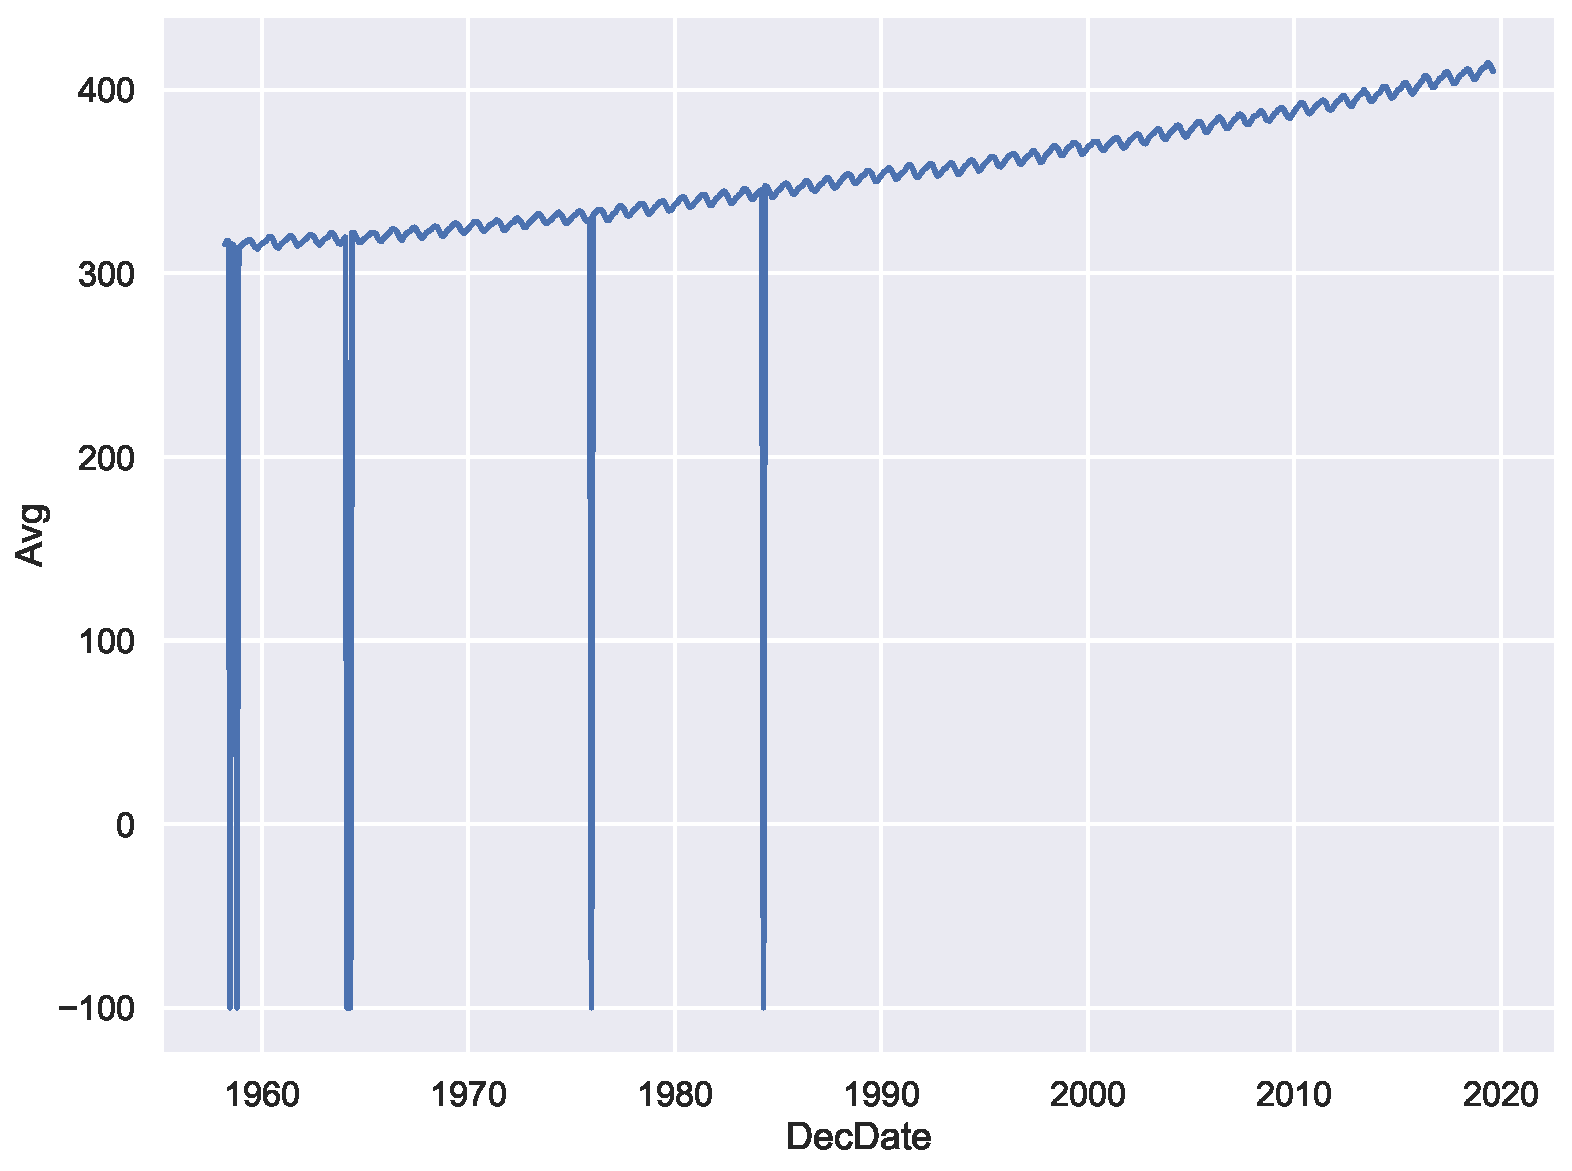
\includegraphics{eda/eda_files/figure-pdf/cell-62-output-1.pdf}

The code above uses the \texttt{seaborn} plotting library (abbreviated
\texttt{sns}). We will cover this in the Visualization lecture, but now
you don't need to worry about how it works!

Yikes! Plotting the data uncovered a problem. The sharp vertical lines
suggest that we have some \textbf{missing values}. What happened here?

\begin{Shaded}
\begin{Highlighting}[]
\NormalTok{co2.head()}
\end{Highlighting}
\end{Shaded}

\begin{longtable}[]{@{}llllllll@{}}
\toprule\noalign{}
& Yr & Mo & DecDate & Avg & Int & Trend & Days \\
\midrule\noalign{}
\endhead
\bottomrule\noalign{}
\endlastfoot
0 & 1958 & 3 & 1958.21 & 315.71 & 315.71 & 314.62 & -1 \\
1 & 1958 & 4 & 1958.29 & 317.45 & 317.45 & 315.29 & -1 \\
2 & 1958 & 5 & 1958.38 & 317.50 & 317.50 & 314.71 & -1 \\
3 & 1958 & 6 & 1958.46 & -99.99 & 317.10 & 314.85 & -1 \\
4 & 1958 & 7 & 1958.54 & 315.86 & 315.86 & 314.98 & -1 \\
\end{longtable}

\begin{Shaded}
\begin{Highlighting}[]
\NormalTok{co2.tail()}
\end{Highlighting}
\end{Shaded}

\begin{longtable}[]{@{}llllllll@{}}
\toprule\noalign{}
& Yr & Mo & DecDate & Avg & Int & Trend & Days \\
\midrule\noalign{}
\endhead
\bottomrule\noalign{}
\endlastfoot
733 & 2019 & 4 & 2019.29 & 413.32 & 413.32 & 410.49 & 26 \\
734 & 2019 & 5 & 2019.38 & 414.66 & 414.66 & 411.20 & 28 \\
735 & 2019 & 6 & 2019.46 & 413.92 & 413.92 & 411.58 & 27 \\
736 & 2019 & 7 & 2019.54 & 411.77 & 411.77 & 411.43 & 23 \\
737 & 2019 & 8 & 2019.62 & 409.95 & 409.95 & 411.84 & 29 \\
\end{longtable}

Some data have unusual values like -1 and -99.99.

Let's check the description at the top of the file again.

\begin{itemize}
\tightlist
\item
  -1 signifies a missing value for the number of days \texttt{Days} the
  equipment was in operation that month.
\item
  -99.99 denotes a missing monthly average \texttt{Avg}
\end{itemize}

How can we fix this? First, let's explore other aspects of our data.
Understanding our data will help us decide what to do with the missing
values.

\subsection{Sanity Checks: Reasoning about the
data}\label{sanity-checks-reasoning-about-the-data}

First, we consider the shape of the data. How many rows should we have?

\begin{itemize}
\tightlist
\item
  If chronological order, we should have one record per month.
\item
  Data from March 1958 to August 2019.
\item
  We should have \$ 12 \times (2019-1957) - 2 - 4 = 738 \$ records.
\end{itemize}

\begin{Shaded}
\begin{Highlighting}[]
\NormalTok{co2.shape}
\end{Highlighting}
\end{Shaded}

\begin{verbatim}
(738, 7)
\end{verbatim}

Nice!! The number of rows (i.e.~records) match our expectations.

Let's now check the quality of each feature.

\subsection{\texorpdfstring{Understanding Missing Value 1:
\texttt{Days}}{Understanding Missing Value 1: Days}}\label{understanding-missing-value-1-days}

\texttt{Days} is a time field, so let's analyze other time fields to see
if there is an explanation for missing values of days of operation.

Let's start with \textbf{months}, \texttt{Mo}.

Are we missing any records? The number of months should have 62 or 61
instances (March 1957-August 2019).

\begin{Shaded}
\begin{Highlighting}[]
\NormalTok{co2[}\StringTok{"Mo"}\NormalTok{].value\_counts().sort\_index()}
\end{Highlighting}
\end{Shaded}

\begin{verbatim}
Mo
1     61
2     61
3     62
4     62
5     62
6     62
7     62
8     62
9     61
10    61
11    61
12    61
Name: count, dtype: int64
\end{verbatim}

As expected Jan, Feb, Sep, Oct, Nov, and Dec have 61 occurrences and the
rest 62.

Next let's explore \textbf{days} \texttt{Days} itself, which is the
number of days that the measurement equipment worked.

\begin{Shaded}
\begin{Highlighting}[]
\NormalTok{sns.displot(co2[}\StringTok{\textquotesingle{}Days\textquotesingle{}}\NormalTok{])}\OperatorTok{;}
\NormalTok{plt.title(}\StringTok{"Distribution of days feature"}\NormalTok{)}\OperatorTok{;} \CommentTok{\# suppresses unneeded plotting output}
\end{Highlighting}
\end{Shaded}

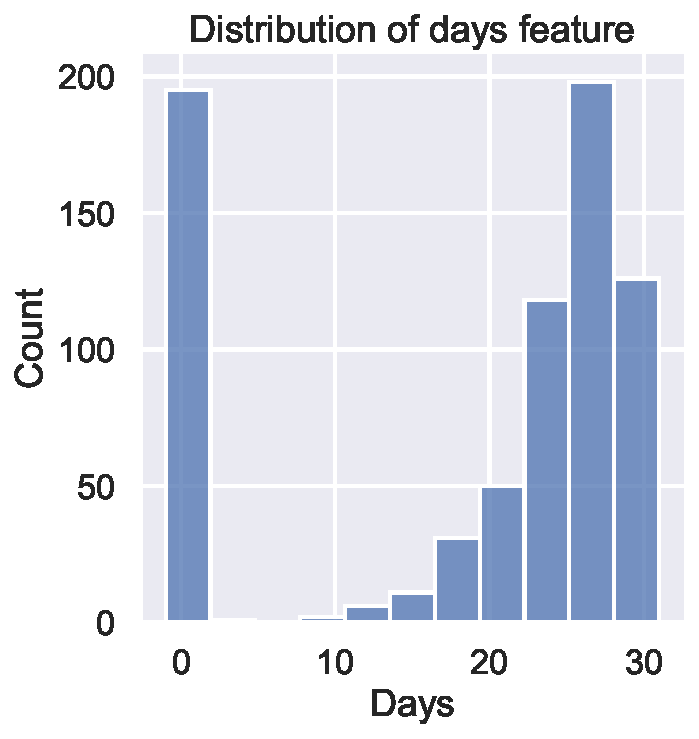
\includegraphics{eda/eda_files/figure-pdf/cell-67-output-1.pdf}

In terms of data quality, a handful of months have averages based on
measurements taken on fewer than half the days. In addition, there are
nearly 200 missing values--\textbf{that's about 27\% of the data}!

Finally, let's check the last time feature, \textbf{year} \texttt{Yr}.

Let's check to see if there is any connection between missing-ness and
the year of the recording.

\begin{Shaded}
\begin{Highlighting}[]
\NormalTok{sns.scatterplot(x}\OperatorTok{=}\StringTok{"Yr"}\NormalTok{, y}\OperatorTok{=}\StringTok{"Days"}\NormalTok{, data}\OperatorTok{=}\NormalTok{co2)}\OperatorTok{;}
\NormalTok{plt.title(}\StringTok{"Day field by Year"}\NormalTok{)}\OperatorTok{;} \CommentTok{\# the ; suppresses output}
\end{Highlighting}
\end{Shaded}

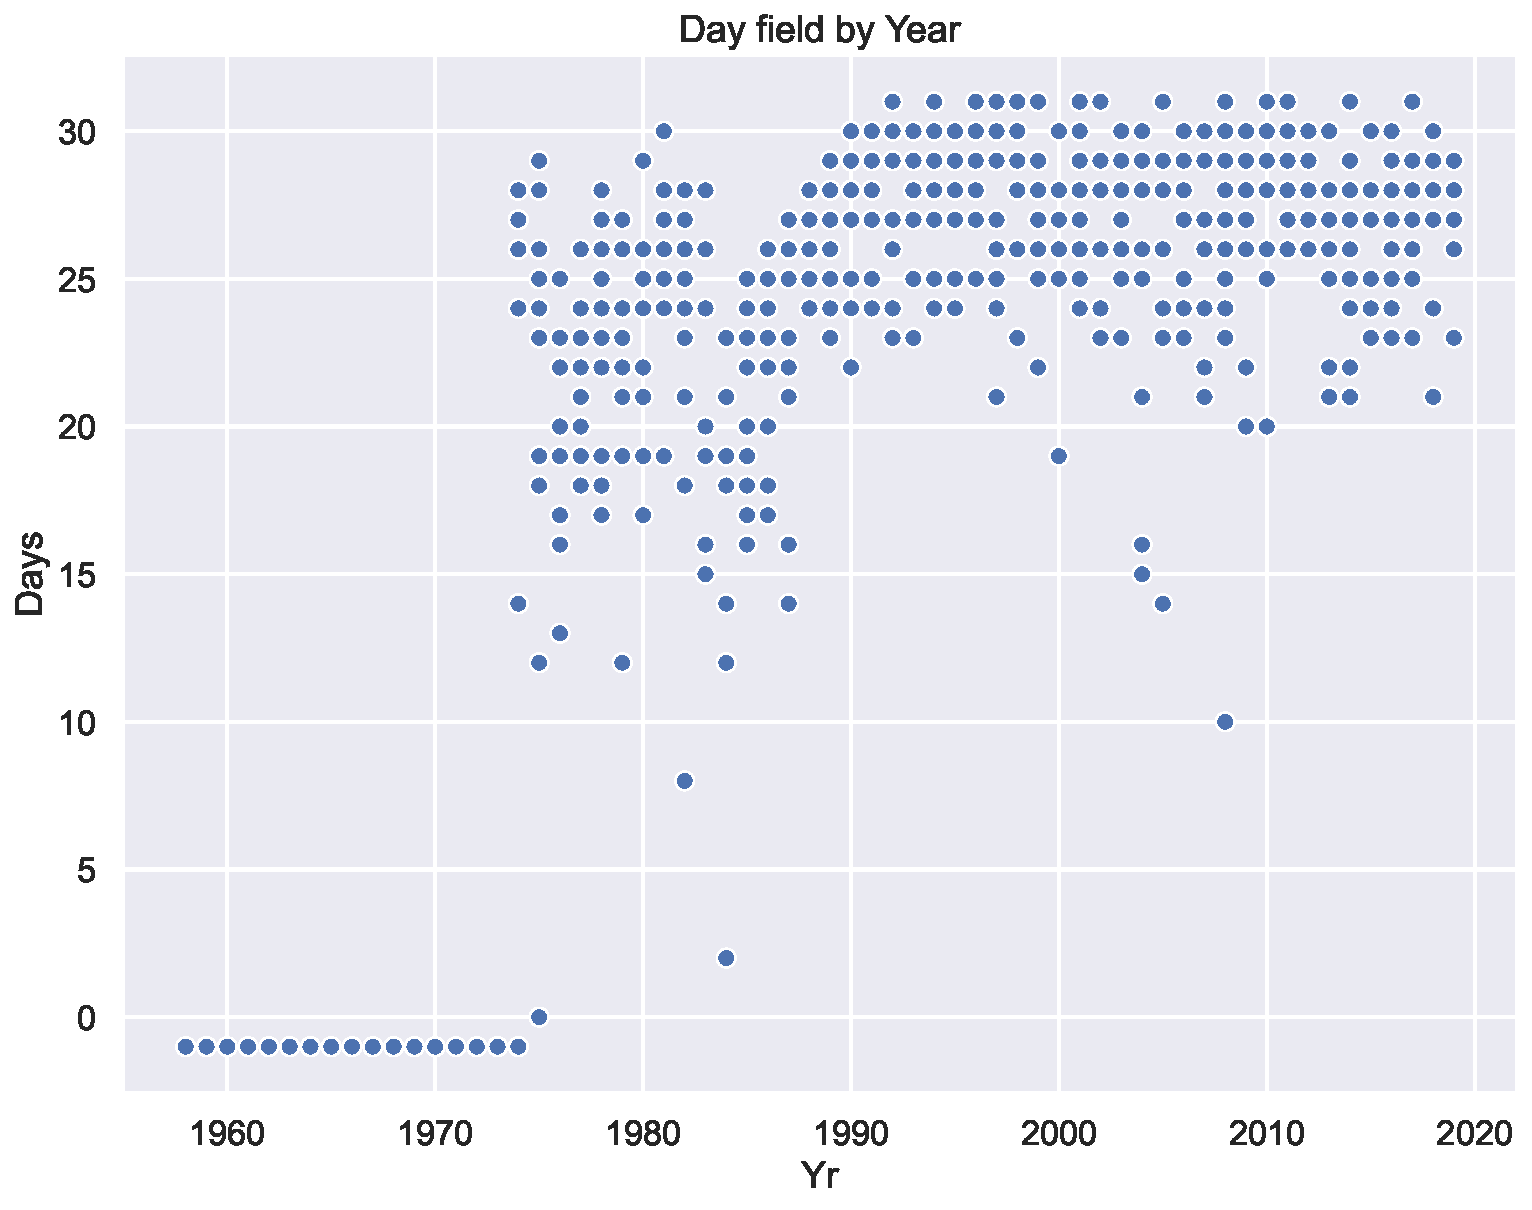
\includegraphics{eda/eda_files/figure-pdf/cell-68-output-1.pdf}

\textbf{Observations}:

\begin{itemize}
\tightlist
\item
  All of the missing data are in the early years of operation.
\item
  It appears there may have been problems with equipment in the mid to
  late 80s.
\end{itemize}

\textbf{Potential Next Steps}:

\begin{itemize}
\tightlist
\item
  Confirm these explanations through documentation about the historical
  readings.
\item
  Maybe drop the earliest recordings? However, we would want to delay
  such action until after we have examined the time trends and assess
  whether there are any potential problems.
\end{itemize}

\subsection{\texorpdfstring{Understanding Missing Value 2:
\texttt{Avg}}{Understanding Missing Value 2: Avg}}\label{understanding-missing-value-2-avg}

Next, let's return to the -99.99 values in \texttt{Avg} to analyze the
overall quality of the CO2 measurements. We'll plot a histogram of the
average CO2 measurements

\begin{Shaded}
\begin{Highlighting}[]
\CommentTok{\# Histograms of average CO2 measurements}
\NormalTok{sns.displot(co2[}\StringTok{\textquotesingle{}Avg\textquotesingle{}}\NormalTok{])}\OperatorTok{;}
\end{Highlighting}
\end{Shaded}

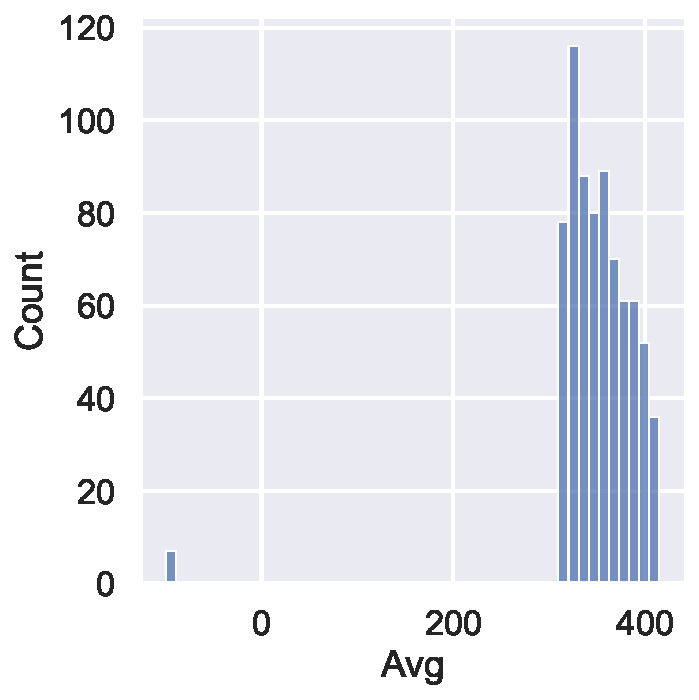
\includegraphics{eda/eda_files/figure-pdf/cell-69-output-1.pdf}

The non-missing values are in the 300-400 range (a regular range of CO2
levels).

We also see that there are only a few missing \texttt{Avg} values
(\textbf{\textless1\% of values}). Let's examine all of them:

\begin{Shaded}
\begin{Highlighting}[]
\NormalTok{co2[co2[}\StringTok{"Avg"}\NormalTok{] }\OperatorTok{\textless{}} \DecValTok{0}\NormalTok{]}
\end{Highlighting}
\end{Shaded}

\begin{longtable}[]{@{}llllllll@{}}
\toprule\noalign{}
& Yr & Mo & DecDate & Avg & Int & Trend & Days \\
\midrule\noalign{}
\endhead
\bottomrule\noalign{}
\endlastfoot
3 & 1958 & 6 & 1958.46 & -99.99 & 317.10 & 314.85 & -1 \\
7 & 1958 & 10 & 1958.79 & -99.99 & 312.66 & 315.61 & -1 \\
71 & 1964 & 2 & 1964.12 & -99.99 & 320.07 & 319.61 & -1 \\
72 & 1964 & 3 & 1964.21 & -99.99 & 320.73 & 319.55 & -1 \\
73 & 1964 & 4 & 1964.29 & -99.99 & 321.77 & 319.48 & -1 \\
213 & 1975 & 12 & 1975.96 & -99.99 & 330.59 & 331.60 & 0 \\
313 & 1984 & 4 & 1984.29 & -99.99 & 346.84 & 344.27 & 2 \\
\end{longtable}

There doesn't seem to be a pattern to these values, other than that most
records also were missing \texttt{Days} data.

\subsection{\texorpdfstring{Drop, \texttt{NaN}, or Impute Missing
\texttt{Avg}
Data?}{Drop, NaN, or Impute Missing Avg Data?}}\label{drop-nan-or-impute-missing-avg-data}

How should we address the invalid \texttt{Avg} data?

\begin{enumerate}
\def\labelenumi{\arabic{enumi}.}
\tightlist
\item
  Drop records
\item
  Set to NaN
\item
  Impute using some strategy
\end{enumerate}

Remember we want to fix the following plot:

\begin{Shaded}
\begin{Highlighting}[]
\NormalTok{sns.lineplot(x}\OperatorTok{=}\StringTok{\textquotesingle{}DecDate\textquotesingle{}}\NormalTok{, y}\OperatorTok{=}\StringTok{\textquotesingle{}Avg\textquotesingle{}}\NormalTok{, data}\OperatorTok{=}\NormalTok{co2)}
\NormalTok{plt.title(}\StringTok{"CO2 Average By Month"}\NormalTok{)}\OperatorTok{;}
\end{Highlighting}
\end{Shaded}

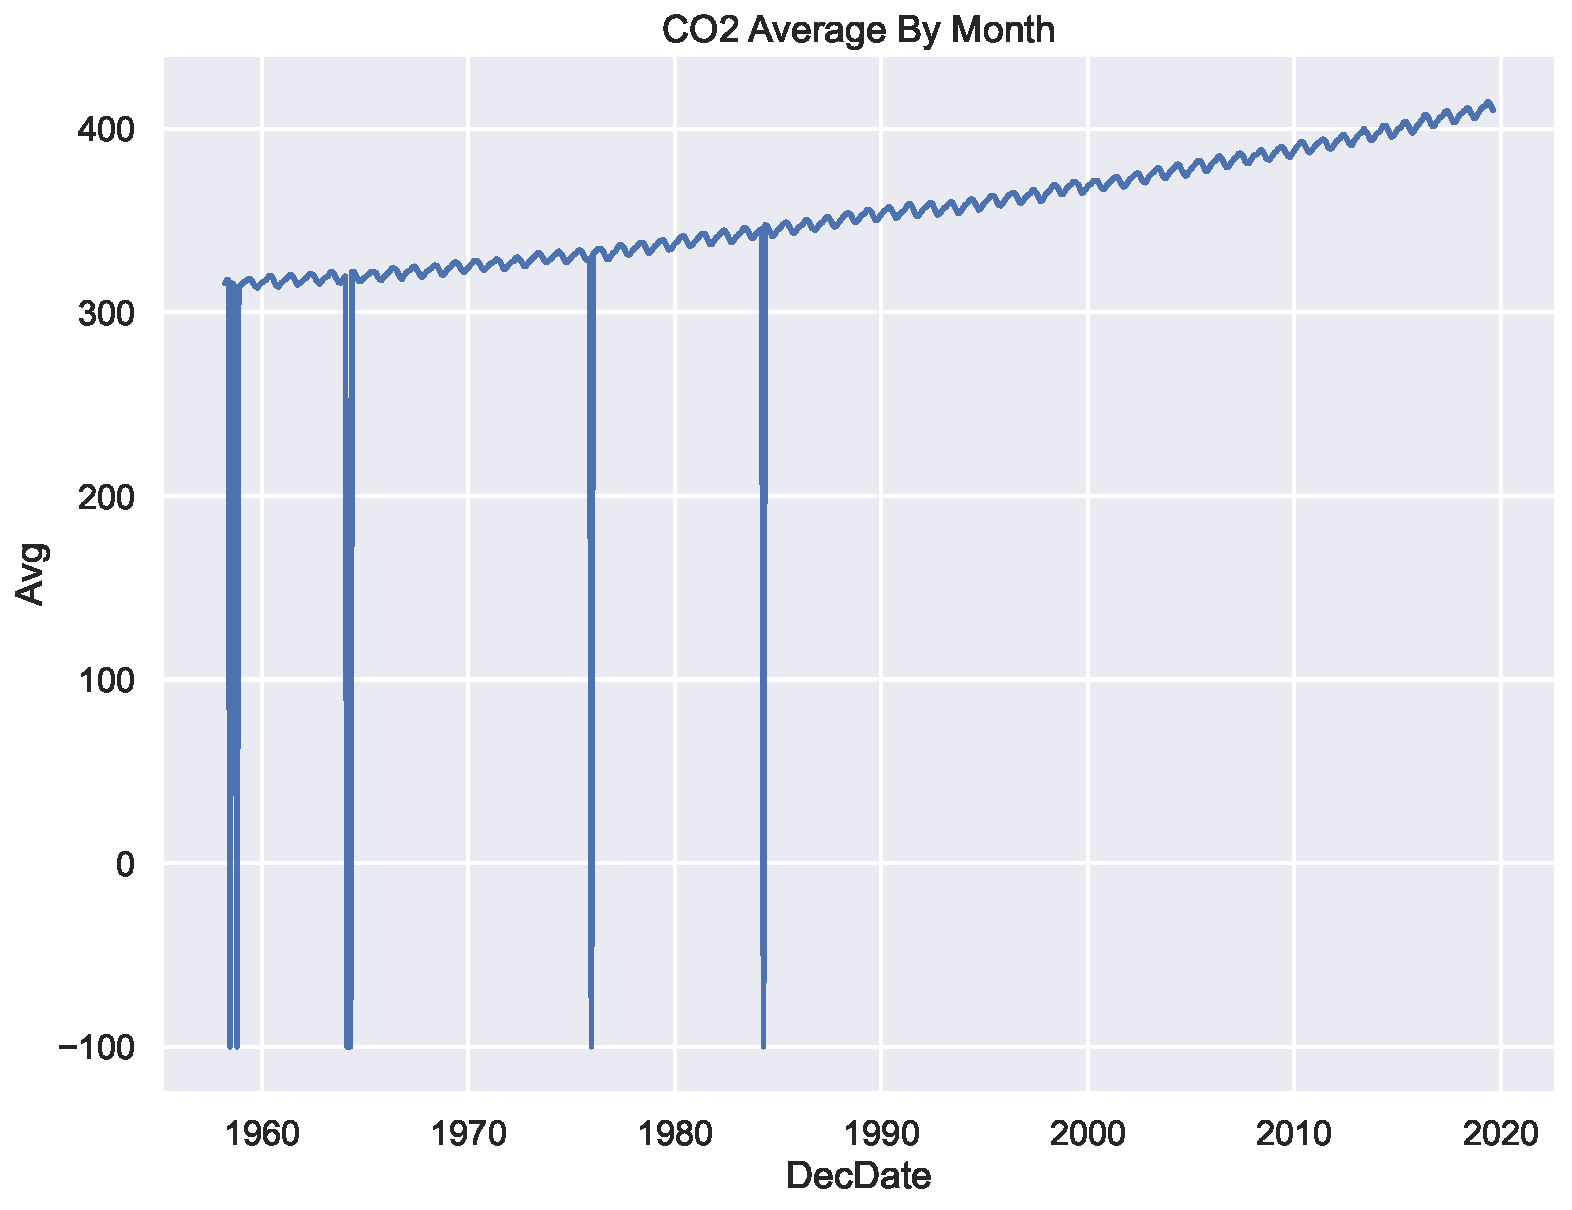
\includegraphics{eda/eda_files/figure-pdf/cell-71-output-1.pdf}

Since we are plotting \texttt{Avg} vs \texttt{DecDate}, we should just
focus on dealing with missing values for \texttt{Avg}.

Let's consider a few options: 1. Drop those records 2. Replace -99.99
with NaN 3. Substitute it with a likely value for the average CO2?

What do you think are the pros and cons of each possible action?

Let's examine each of these three options.

\begin{Shaded}
\begin{Highlighting}[]
\CommentTok{\# 1. Drop missing values}
\NormalTok{co2\_drop }\OperatorTok{=}\NormalTok{ co2[co2[}\StringTok{\textquotesingle{}Avg\textquotesingle{}}\NormalTok{] }\OperatorTok{\textgreater{}} \DecValTok{0}\NormalTok{]}
\NormalTok{co2\_drop.head()}
\end{Highlighting}
\end{Shaded}

\begin{longtable}[]{@{}llllllll@{}}
\toprule\noalign{}
& Yr & Mo & DecDate & Avg & Int & Trend & Days \\
\midrule\noalign{}
\endhead
\bottomrule\noalign{}
\endlastfoot
0 & 1958 & 3 & 1958.21 & 315.71 & 315.71 & 314.62 & -1 \\
1 & 1958 & 4 & 1958.29 & 317.45 & 317.45 & 315.29 & -1 \\
2 & 1958 & 5 & 1958.38 & 317.50 & 317.50 & 314.71 & -1 \\
4 & 1958 & 7 & 1958.54 & 315.86 & 315.86 & 314.98 & -1 \\
5 & 1958 & 8 & 1958.62 & 314.93 & 314.93 & 315.94 & -1 \\
\end{longtable}

\begin{Shaded}
\begin{Highlighting}[]
\CommentTok{\# 2. Replace NaN with {-}99.99}
\NormalTok{co2\_NA }\OperatorTok{=}\NormalTok{ co2.replace(}\OperatorTok{{-}}\FloatTok{99.99}\NormalTok{, np.NaN)}
\NormalTok{co2\_NA.head()}
\end{Highlighting}
\end{Shaded}

\begin{longtable}[]{@{}llllllll@{}}
\toprule\noalign{}
& Yr & Mo & DecDate & Avg & Int & Trend & Days \\
\midrule\noalign{}
\endhead
\bottomrule\noalign{}
\endlastfoot
0 & 1958 & 3 & 1958.21 & 315.71 & 315.71 & 314.62 & -1 \\
1 & 1958 & 4 & 1958.29 & 317.45 & 317.45 & 315.29 & -1 \\
2 & 1958 & 5 & 1958.38 & 317.50 & 317.50 & 314.71 & -1 \\
3 & 1958 & 6 & 1958.46 & NaN & 317.10 & 314.85 & -1 \\
4 & 1958 & 7 & 1958.54 & 315.86 & 315.86 & 314.98 & -1 \\
\end{longtable}

We'll also use a third version of the data.

First, we note that the dataset already comes with a \textbf{substitute
value} for the -99.99.

From the file description:

\begin{quote}
The \texttt{interpolated} column includes average values from the
preceding column (\texttt{average}) and \textbf{interpolated values}
where data are missing. Interpolated values are computed in two
steps\ldots{}
\end{quote}

The \texttt{Int} feature has values that exactly match those in
\texttt{Avg}, except when \texttt{Avg} is -99.99, and then a
\textbf{reasonable} estimate is used instead.

So, the third version of our data will use the \texttt{Int} feature
instead of \texttt{Avg}.

\begin{Shaded}
\begin{Highlighting}[]
\CommentTok{\# 3. Use interpolated column which estimates missing Avg values}
\NormalTok{co2\_impute }\OperatorTok{=}\NormalTok{ co2.copy()}
\NormalTok{co2\_impute[}\StringTok{\textquotesingle{}Avg\textquotesingle{}}\NormalTok{] }\OperatorTok{=}\NormalTok{ co2[}\StringTok{\textquotesingle{}Int\textquotesingle{}}\NormalTok{]}
\NormalTok{co2\_impute.head()}
\end{Highlighting}
\end{Shaded}

\begin{longtable}[]{@{}llllllll@{}}
\toprule\noalign{}
& Yr & Mo & DecDate & Avg & Int & Trend & Days \\
\midrule\noalign{}
\endhead
\bottomrule\noalign{}
\endlastfoot
0 & 1958 & 3 & 1958.21 & 315.71 & 315.71 & 314.62 & -1 \\
1 & 1958 & 4 & 1958.29 & 317.45 & 317.45 & 315.29 & -1 \\
2 & 1958 & 5 & 1958.38 & 317.50 & 317.50 & 314.71 & -1 \\
3 & 1958 & 6 & 1958.46 & 317.10 & 317.10 & 314.85 & -1 \\
4 & 1958 & 7 & 1958.54 & 315.86 & 315.86 & 314.98 & -1 \\
\end{longtable}

What's a \textbf{reasonable} estimate?

To answer this question, let's zoom in on a short time period, say the
measurements in 1958 (where we know we have two missing values).

\begin{Shaded}
\begin{Highlighting}[]
\CommentTok{\# results of plotting data in 1958}

\KeywordTok{def}\NormalTok{ line\_and\_points(data, ax, title):}
    \CommentTok{\# assumes single year, hence Mo}
\NormalTok{    ax.plot(}\StringTok{\textquotesingle{}Mo\textquotesingle{}}\NormalTok{, }\StringTok{\textquotesingle{}Avg\textquotesingle{}}\NormalTok{, data}\OperatorTok{=}\NormalTok{data)}
\NormalTok{    ax.scatter(}\StringTok{\textquotesingle{}Mo\textquotesingle{}}\NormalTok{, }\StringTok{\textquotesingle{}Avg\textquotesingle{}}\NormalTok{, data}\OperatorTok{=}\NormalTok{data)}
\NormalTok{    ax.set\_xlim(}\DecValTok{2}\NormalTok{, }\DecValTok{13}\NormalTok{)}
\NormalTok{    ax.set\_title(title)}
\NormalTok{    ax.set\_xticks(np.arange(}\DecValTok{3}\NormalTok{, }\DecValTok{13}\NormalTok{))}

\KeywordTok{def}\NormalTok{ data\_year(data, year):}
    \ControlFlowTok{return}\NormalTok{ data[data[}\StringTok{"Yr"}\NormalTok{] }\OperatorTok{==} \DecValTok{1958}\NormalTok{]}
    
\CommentTok{\# uses matplotlib subplots}
\CommentTok{\# you may see more next week; focus on output for now}
\NormalTok{fig, axes }\OperatorTok{=}\NormalTok{ plt.subplots(ncols }\OperatorTok{=} \DecValTok{3}\NormalTok{, figsize}\OperatorTok{=}\NormalTok{(}\DecValTok{12}\NormalTok{, }\DecValTok{4}\NormalTok{), sharey}\OperatorTok{=}\VariableTok{True}\NormalTok{)}

\NormalTok{year }\OperatorTok{=} \DecValTok{1958}
\NormalTok{line\_and\_points(data\_year(co2\_drop, year), axes[}\DecValTok{0}\NormalTok{], title}\OperatorTok{=}\StringTok{"1. Drop Missing"}\NormalTok{)}
\NormalTok{line\_and\_points(data\_year(co2\_NA, year), axes[}\DecValTok{1}\NormalTok{], title}\OperatorTok{=}\StringTok{"2. Missing Set to NaN"}\NormalTok{)}
\NormalTok{line\_and\_points(data\_year(co2\_impute, year), axes[}\DecValTok{2}\NormalTok{], title}\OperatorTok{=}\StringTok{"3. Missing Interpolated"}\NormalTok{)}

\NormalTok{fig.suptitle(}\SpecialStringTok{f"Monthly Averages for }\SpecialCharTok{\{}\NormalTok{year}\SpecialCharTok{\}}\SpecialStringTok{"}\NormalTok{)}
\NormalTok{plt.tight\_layout()}
\end{Highlighting}
\end{Shaded}

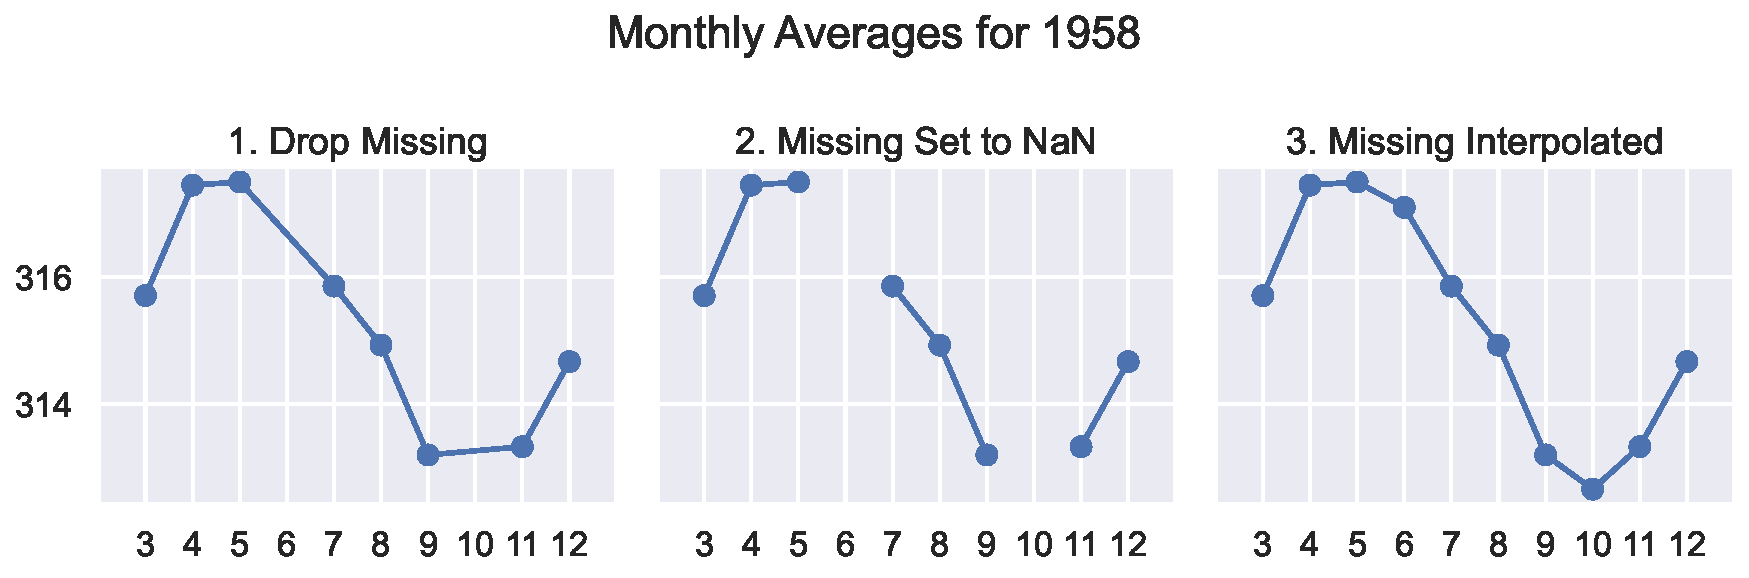
\includegraphics{eda/eda_files/figure-pdf/cell-75-output-1.pdf}

In the big picture since there are only 7 \texttt{Avg} values missing
(\textbf{\textless1\%} of 738 months), any of these approaches would
work.

However there is some appeal to \textbf{option C, Imputing}:

\begin{itemize}
\tightlist
\item
  Shows seasonal trends for CO2
\item
  We are plotting all months in our data as a line plot
\end{itemize}

Let's replot our original figure with option 3:

\begin{Shaded}
\begin{Highlighting}[]
\NormalTok{sns.lineplot(x}\OperatorTok{=}\StringTok{\textquotesingle{}DecDate\textquotesingle{}}\NormalTok{, y}\OperatorTok{=}\StringTok{\textquotesingle{}Avg\textquotesingle{}}\NormalTok{, data}\OperatorTok{=}\NormalTok{co2\_impute)}
\NormalTok{plt.title(}\StringTok{"CO2 Average By Month, Imputed"}\NormalTok{)}\OperatorTok{;}
\end{Highlighting}
\end{Shaded}

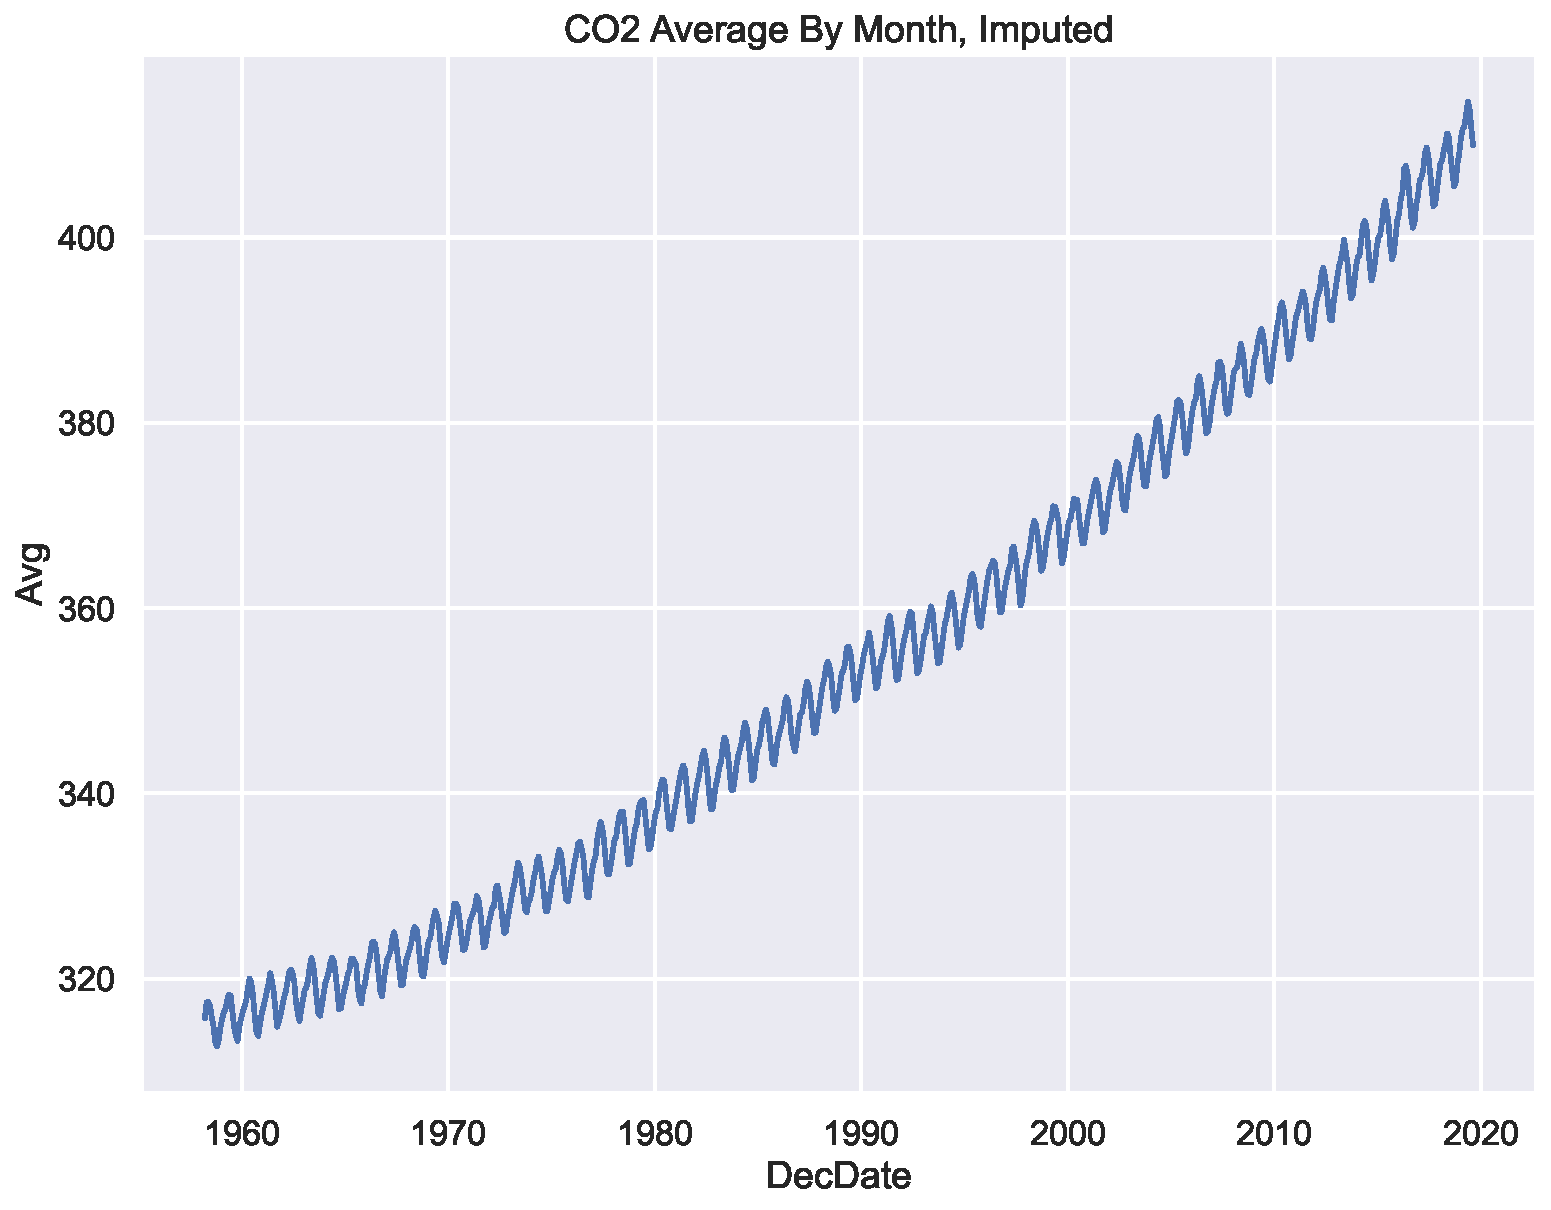
\includegraphics{eda/eda_files/figure-pdf/cell-76-output-1.pdf}

Looks pretty close to what we see on the NOAA
\href{https://gml.noaa.gov/ccgg/trends/}{website}!

\subsection{Presenting the Data: A Discussion on Data
Granularity}\label{presenting-the-data-a-discussion-on-data-granularity}

From the description:

\begin{itemize}
\tightlist
\item
  Monthly measurements are averages of average day measurements.
\item
  The NOAA GML website has datasets for daily/hourly measurements too.
\end{itemize}

The data you present depends on your research question.

\textbf{How do CO2 levels vary by season?}

\begin{itemize}
\tightlist
\item
  You might want to keep average monthly data.
\end{itemize}

\textbf{Are CO2 levels rising over the past 50+ years, consistent with
global warming predictions?}

\begin{itemize}
\tightlist
\item
  You might be happier with a \textbf{coarser granularity} of average
  year data!
\end{itemize}

\begin{Shaded}
\begin{Highlighting}[]
\NormalTok{co2\_year }\OperatorTok{=}\NormalTok{ co2\_impute.groupby(}\StringTok{\textquotesingle{}Yr\textquotesingle{}}\NormalTok{).mean()}
\NormalTok{sns.lineplot(x}\OperatorTok{=}\StringTok{\textquotesingle{}Yr\textquotesingle{}}\NormalTok{, y}\OperatorTok{=}\StringTok{\textquotesingle{}Avg\textquotesingle{}}\NormalTok{, data}\OperatorTok{=}\NormalTok{co2\_year)}
\NormalTok{plt.title(}\StringTok{"CO2 Average By Year"}\NormalTok{)}\OperatorTok{;}
\end{Highlighting}
\end{Shaded}

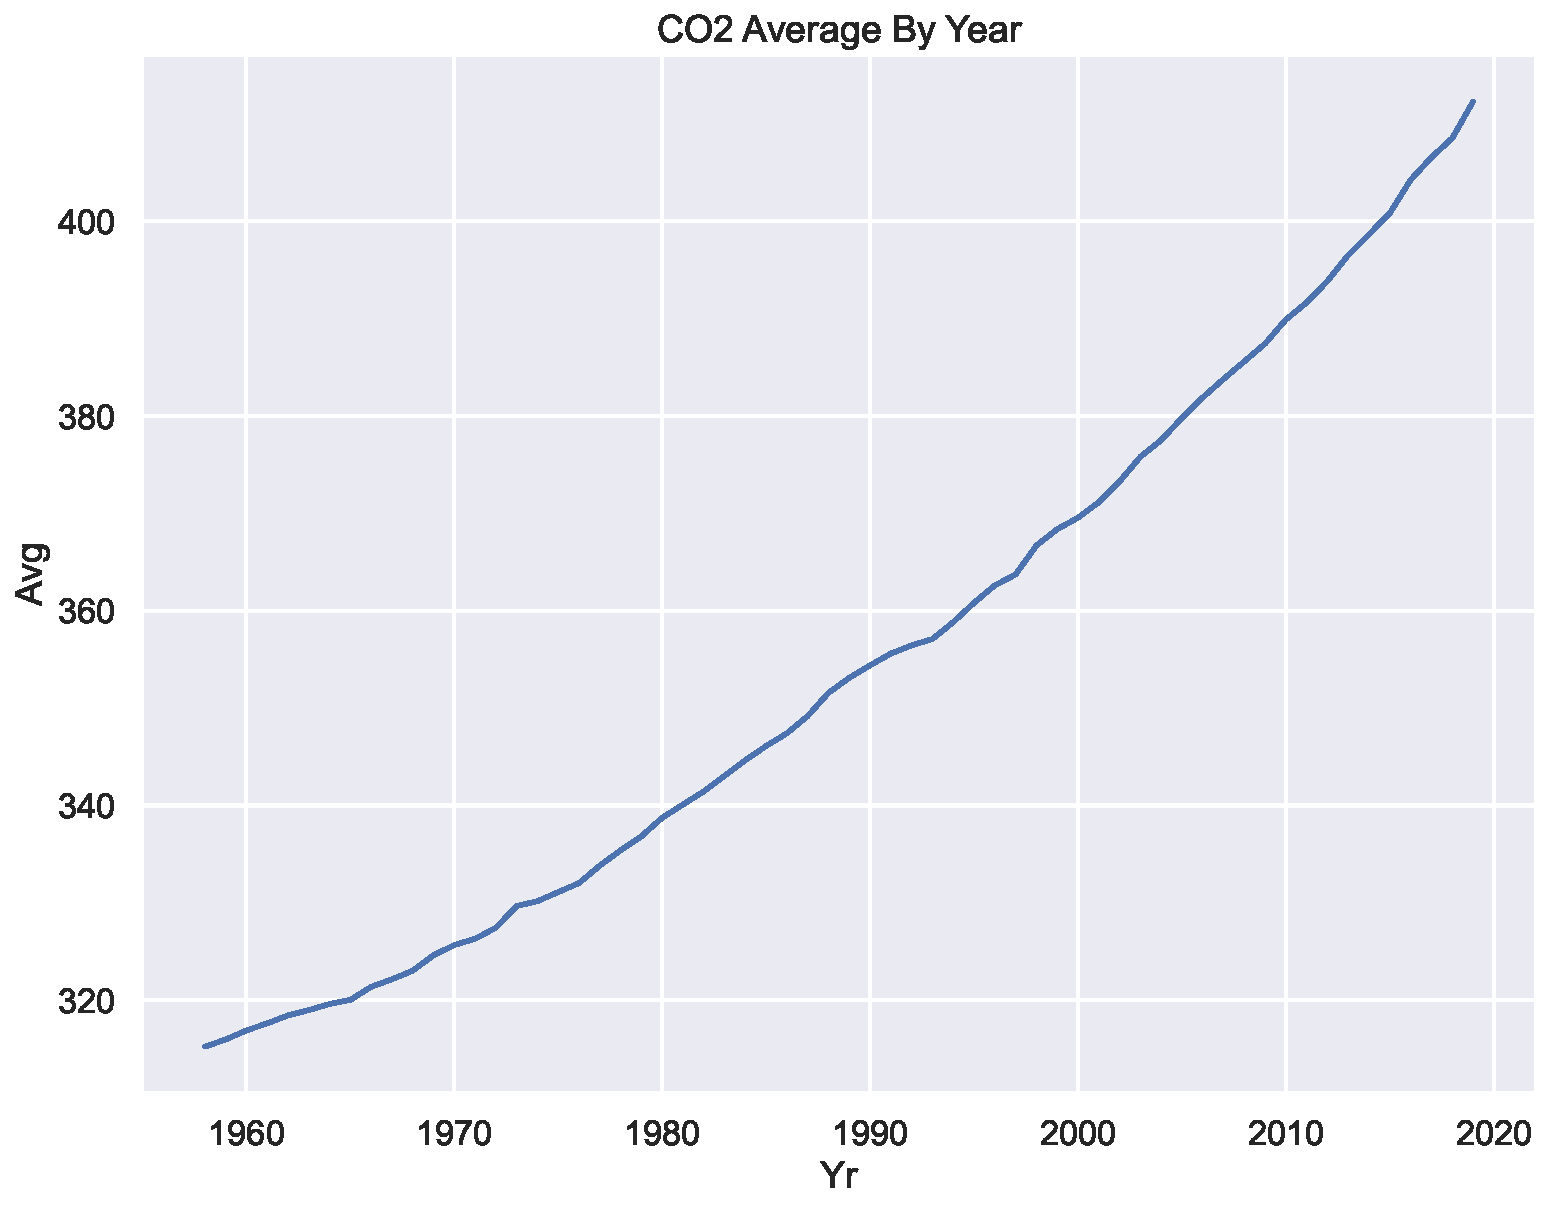
\includegraphics{eda/eda_files/figure-pdf/cell-77-output-1.pdf}

Indeed, we see a rise by nearly 100 ppm of CO2 since Mauna Loa began
recording in 1958.

\section{Summary}\label{summary}

We went over a lot of content this lecture; let's summarize the most
important points:

\subsection{Dealing with Missing
Values}\label{dealing-with-missing-values}

There are a few options we can take to deal with missing data:

\begin{itemize}
\tightlist
\item
  Drop missing records
\item
  Keep \texttt{NaN} missing values
\item
  Impute using an interpolated column
\end{itemize}

\subsection{EDA and Data Wrangling}\label{eda-and-data-wrangling}

There are several ways to approach EDA and Data Wrangling:

\begin{itemize}
\tightlist
\item
  Examine the \textbf{data and metadata}: what is the date, size,
  organization, and structure of the data?
\item
  Examine each \textbf{field/attribute/dimension} individually.
\item
  Examine pairs of related dimensions (e.g.~breaking down grades by
  major).
\item
  Along the way, we can:

  \begin{itemize}
  \tightlist
  \item
    \textbf{Visualize} or summarize the data.
  \item
    \textbf{Validate assumptions} about data and its collection process.
    Pay particular attention to when the data was collected.
  \item
    Identify and \textbf{address anomalies}.
  \item
    Apply data transformations and corrections (we'll cover this in the
    upcoming lecture).
  \item
    \textbf{Record everything you do!} Developing in Jupyter Notebook
    promotes \emph{reproducibility} of your own work!
  \end{itemize}
\end{itemize}

\bookmarksetup{startatroot}

\chapter{Regular Expressions}\label{regular-expressions}

\begin{tcolorbox}[enhanced jigsaw, colbacktitle=quarto-callout-note-color!10!white, colframe=quarto-callout-note-color-frame, bottomtitle=1mm, colback=white, arc=.35mm, rightrule=.15mm, opacityback=0, toptitle=1mm, leftrule=.75mm, bottomrule=.15mm, coltitle=black, titlerule=0mm, breakable, left=2mm, opacitybacktitle=0.6, toprule=.15mm, title=\textcolor{quarto-callout-note-color}{\faInfo}\hspace{0.5em}{Learning Outcomes}]

\begin{itemize}
\tightlist
\item
  Understand Python string manipulation, \texttt{pandas} \texttt{Series}
  methods
\item
  Parse and create regex, with a reference table
\item
  Use vocabulary (closure, metacharacters, groups, etc.) to describe
  regex metacharacters
\end{itemize}

\end{tcolorbox}

\section{Why Work with Text?}\label{why-work-with-text}

Last lecture, we learned of the difference between quantitative and
qualitative variable types. The latter includes string data --- the
primary focus of lecture 6. In this note, we'll discuss the necessary
tools to manipulate text: \texttt{python} string manipulation and
regular expressions.

There are two main reasons for working with text.

\begin{enumerate}
\def\labelenumi{\arabic{enumi}.}
\tightlist
\item
  Canonicalization: Convert data that has multiple formats into a
  standard form.

  \begin{itemize}
  \tightlist
  \item
    By manipulating text, we can join tables with mismatched string
    labels.
  \end{itemize}
\item
  Extract information into a new feature.

  \begin{itemize}
  \tightlist
  \item
    For example, we can extract date and time features from text.
  \end{itemize}
\end{enumerate}

\section{Python String Methods}\label{python-string-methods}

First, we'll introduce a few methods useful for string manipulation. The
following table includes a number of string operations supported by
\texttt{python} and \texttt{pandas}. The \texttt{python} functions
operate on a single string, while their equivalent in \texttt{pandas}
are \textbf{vectorized} --- they operate on a \texttt{Series} of string
data.

\begin{longtable}[]{@{}
  >{\raggedright\arraybackslash}p{(\columnwidth - 4\tabcolsep) * \real{0.3333}}
  >{\raggedright\arraybackslash}p{(\columnwidth - 4\tabcolsep) * \real{0.2500}}
  >{\raggedright\arraybackslash}p{(\columnwidth - 4\tabcolsep) * \real{0.3889}}@{}}
\toprule\noalign{}
\begin{minipage}[b]{\linewidth}\raggedright
Operation
\end{minipage} & \begin{minipage}[b]{\linewidth}\raggedright
Python
\end{minipage} & \begin{minipage}[b]{\linewidth}\raggedright
\texttt{Pandas} (\texttt{Series})
\end{minipage} \\
\midrule\noalign{}
\endhead
\bottomrule\noalign{}
\endlastfoot
Transformation & \begin{minipage}[t]{\linewidth}\raggedright
\begin{itemize}
\tightlist
\item
  \texttt{s.lower()}
\item
  \texttt{s.upper()}
\end{itemize}
\end{minipage} & \begin{minipage}[t]{\linewidth}\raggedright
\begin{itemize}
\tightlist
\item
  \texttt{ser.str.lower()}
\item
  \texttt{ser.str.upper()}
\end{itemize}
\end{minipage} \\
Replacement + Deletion & \begin{minipage}[t]{\linewidth}\raggedright
\begin{itemize}
\tightlist
\item
  \texttt{s.replace(\_)}
\end{itemize}
\end{minipage} & \begin{minipage}[t]{\linewidth}\raggedright
\begin{itemize}
\tightlist
\item
  \texttt{ser.str.replace(\_)}
\end{itemize}
\end{minipage} \\
Split & \begin{minipage}[t]{\linewidth}\raggedright
\begin{itemize}
\tightlist
\item
  \texttt{s.split(\_)}
\end{itemize}
\end{minipage} & \begin{minipage}[t]{\linewidth}\raggedright
\begin{itemize}
\tightlist
\item
  \texttt{ser.str.split(\_)}
\end{itemize}
\end{minipage} \\
Substring & \begin{minipage}[t]{\linewidth}\raggedright
\begin{itemize}
\tightlist
\item
  \texttt{s{[}1:4{]}}
\end{itemize}
\end{minipage} & \begin{minipage}[t]{\linewidth}\raggedright
\begin{itemize}
\tightlist
\item
  \texttt{ser.str{[}1:4{]}}
\end{itemize}
\end{minipage} \\
Membership & \begin{minipage}[t]{\linewidth}\raggedright
\begin{itemize}
\tightlist
\item
  \texttt{\textquotesingle{}\_\textquotesingle{}\ in\ s}
\end{itemize}
\end{minipage} & \begin{minipage}[t]{\linewidth}\raggedright
\begin{itemize}
\tightlist
\item
  \texttt{ser.str.contains(\_)}
\end{itemize}
\end{minipage} \\
Length & \begin{minipage}[t]{\linewidth}\raggedright
\begin{itemize}
\tightlist
\item
  \texttt{len(s)}
\end{itemize}
\end{minipage} & \begin{minipage}[t]{\linewidth}\raggedright
\begin{itemize}
\tightlist
\item
  \texttt{ser.str.len()}
\end{itemize}
\end{minipage} \\
\end{longtable}

We'll discuss the differences between \texttt{python} string functions
and \texttt{pandas} \texttt{Series} methods in the following section on
canonicalization.

\subsection{Canonicalization}\label{canonicalization}

Assume we want to merge the given tables.

\begin{Shaded}
\begin{Highlighting}[]
\ImportTok{import}\NormalTok{ pandas }\ImportTok{as}\NormalTok{ pd}

\ControlFlowTok{with} \BuiltInTok{open}\NormalTok{(}\StringTok{\textquotesingle{}data/county\_and\_state.csv\textquotesingle{}}\NormalTok{) }\ImportTok{as}\NormalTok{ f:}
\NormalTok{    county\_and\_state }\OperatorTok{=}\NormalTok{ pd.read\_csv(f)}
    
\ControlFlowTok{with} \BuiltInTok{open}\NormalTok{(}\StringTok{\textquotesingle{}data/county\_and\_population.csv\textquotesingle{}}\NormalTok{) }\ImportTok{as}\NormalTok{ f:}
\NormalTok{    county\_and\_pop }\OperatorTok{=}\NormalTok{ pd.read\_csv(f)}
\end{Highlighting}
\end{Shaded}

\begin{Shaded}
\begin{Highlighting}[]
\NormalTok{display(county\_and\_state), display(county\_and\_pop)}\OperatorTok{;}
\end{Highlighting}
\end{Shaded}

\begin{longtable}[]{@{}lll@{}}
\toprule\noalign{}
& County & State \\
\midrule\noalign{}
\endhead
\bottomrule\noalign{}
\endlastfoot
0 & De Witt County & IL \\
1 & Lac qui Parle County & MN \\
2 & Lewis and Clark County & MT \\
3 & St John the Baptist Parish & LS \\
\end{longtable}

\begin{longtable}[]{@{}lll@{}}
\toprule\noalign{}
& County & Population \\
\midrule\noalign{}
\endhead
\bottomrule\noalign{}
\endlastfoot
0 & DeWitt & 16798 \\
1 & Lac Qui Parle & 8067 \\
2 & Lewis \& Clark & 55716 \\
3 & St. John the Baptist & 43044 \\
\end{longtable}

Last time, we used a \textbf{primary key} and \textbf{foreign key} to
join two tables. While neither of these keys exist in our
\texttt{DataFrame}s, the \texttt{"County"} columns look similar enough.
Can we convert these columns into one standard, canonical form to merge
the two tables?

\subsubsection{\texorpdfstring{Canonicalization with \texttt{python}
String
Manipulation}{Canonicalization with python String Manipulation}}\label{canonicalization-with-python-string-manipulation}

The following function uses \texttt{python} string manipulation to
convert a single county name into canonical form. It does so by
eliminating whitespace, punctuation, and unnecessary text.

\begin{Shaded}
\begin{Highlighting}[]
\KeywordTok{def}\NormalTok{ canonicalize\_county(county\_name):}
    \ControlFlowTok{return}\NormalTok{ (}
\NormalTok{        county\_name}
\NormalTok{            .lower()}
\NormalTok{            .replace(}\StringTok{\textquotesingle{} \textquotesingle{}}\NormalTok{, }\StringTok{\textquotesingle{}\textquotesingle{}}\NormalTok{)}
\NormalTok{            .replace(}\StringTok{\textquotesingle{}\&\textquotesingle{}}\NormalTok{, }\StringTok{\textquotesingle{}and\textquotesingle{}}\NormalTok{)}
\NormalTok{            .replace(}\StringTok{\textquotesingle{}.\textquotesingle{}}\NormalTok{, }\StringTok{\textquotesingle{}\textquotesingle{}}\NormalTok{)}
\NormalTok{            .replace(}\StringTok{\textquotesingle{}county\textquotesingle{}}\NormalTok{, }\StringTok{\textquotesingle{}\textquotesingle{}}\NormalTok{)}
\NormalTok{            .replace(}\StringTok{\textquotesingle{}parish\textquotesingle{}}\NormalTok{, }\StringTok{\textquotesingle{}\textquotesingle{}}\NormalTok{)}
\NormalTok{    )}

\NormalTok{canonicalize\_county(}\StringTok{"St. John the Baptist"}\NormalTok{)}
\end{Highlighting}
\end{Shaded}

\begin{verbatim}
'stjohnthebaptist'
\end{verbatim}

We will use the \texttt{pandas} \texttt{map} function to apply the
\texttt{canonicalize\_county} function to every row in both
\texttt{DataFrame}s. In doing so, we'll create a new column in each
called \texttt{clean\_county\_python} with the canonical form.

\begin{Shaded}
\begin{Highlighting}[]
\NormalTok{county\_and\_pop[}\StringTok{\textquotesingle{}clean\_county\_python\textquotesingle{}}\NormalTok{] }\OperatorTok{=}\NormalTok{ county\_and\_pop[}\StringTok{\textquotesingle{}County\textquotesingle{}}\NormalTok{].}\BuiltInTok{map}\NormalTok{(canonicalize\_county)}
\NormalTok{county\_and\_state[}\StringTok{\textquotesingle{}clean\_county\_python\textquotesingle{}}\NormalTok{] }\OperatorTok{=}\NormalTok{ county\_and\_state[}\StringTok{\textquotesingle{}County\textquotesingle{}}\NormalTok{].}\BuiltInTok{map}\NormalTok{(canonicalize\_county)}
\NormalTok{display(county\_and\_state), display(county\_and\_pop)}\OperatorTok{;}
\end{Highlighting}
\end{Shaded}

\begin{longtable}[]{@{}llll@{}}
\toprule\noalign{}
& County & State & clean\_county\_python \\
\midrule\noalign{}
\endhead
\bottomrule\noalign{}
\endlastfoot
0 & De Witt County & IL & dewitt \\
1 & Lac qui Parle County & MN & lacquiparle \\
2 & Lewis and Clark County & MT & lewisandclark \\
3 & St John the Baptist Parish & LS & stjohnthebaptist \\
\end{longtable}

\begin{longtable}[]{@{}llll@{}}
\toprule\noalign{}
& County & Population & clean\_county\_python \\
\midrule\noalign{}
\endhead
\bottomrule\noalign{}
\endlastfoot
0 & DeWitt & 16798 & dewitt \\
1 & Lac Qui Parle & 8067 & lacquiparle \\
2 & Lewis \& Clark & 55716 & lewisandclark \\
3 & St. John the Baptist & 43044 & stjohnthebaptist \\
\end{longtable}

\subsubsection{Canonicalization with Pandas Series
Methods}\label{canonicalization-with-pandas-series-methods}

Alternatively, we can use \texttt{pandas} \texttt{Series} methods to
create this standardized column. To do so, we must call the
\texttt{.str} attribute of our \texttt{Series} object prior to calling
any methods, like \texttt{.lower} and \texttt{.replace}. Notice how
these method names match their equivalent built-in Python string
functions.

Chaining multiple \texttt{Series} methods in this manner eliminates the
need to use the \texttt{map} function (as this code is vectorized).

\begin{Shaded}
\begin{Highlighting}[]
\KeywordTok{def}\NormalTok{ canonicalize\_county\_series(county\_series):}
    \ControlFlowTok{return}\NormalTok{ (}
\NormalTok{        county\_series}
\NormalTok{            .}\BuiltInTok{str}\NormalTok{.lower()}
\NormalTok{            .}\BuiltInTok{str}\NormalTok{.replace(}\StringTok{\textquotesingle{} \textquotesingle{}}\NormalTok{, }\StringTok{\textquotesingle{}\textquotesingle{}}\NormalTok{)}
\NormalTok{            .}\BuiltInTok{str}\NormalTok{.replace(}\StringTok{\textquotesingle{}\&\textquotesingle{}}\NormalTok{, }\StringTok{\textquotesingle{}and\textquotesingle{}}\NormalTok{)}
\NormalTok{            .}\BuiltInTok{str}\NormalTok{.replace(}\StringTok{\textquotesingle{}.\textquotesingle{}}\NormalTok{, }\StringTok{\textquotesingle{}\textquotesingle{}}\NormalTok{)}
\NormalTok{            .}\BuiltInTok{str}\NormalTok{.replace(}\StringTok{\textquotesingle{}county\textquotesingle{}}\NormalTok{, }\StringTok{\textquotesingle{}\textquotesingle{}}\NormalTok{)}
\NormalTok{            .}\BuiltInTok{str}\NormalTok{.replace(}\StringTok{\textquotesingle{}parish\textquotesingle{}}\NormalTok{, }\StringTok{\textquotesingle{}\textquotesingle{}}\NormalTok{)}
\NormalTok{    )}

\NormalTok{county\_and\_pop[}\StringTok{\textquotesingle{}clean\_county\_pandas\textquotesingle{}}\NormalTok{] }\OperatorTok{=}\NormalTok{ canonicalize\_county\_series(county\_and\_pop[}\StringTok{\textquotesingle{}County\textquotesingle{}}\NormalTok{])}
\NormalTok{county\_and\_state[}\StringTok{\textquotesingle{}clean\_county\_pandas\textquotesingle{}}\NormalTok{] }\OperatorTok{=}\NormalTok{ canonicalize\_county\_series(county\_and\_state[}\StringTok{\textquotesingle{}County\textquotesingle{}}\NormalTok{])}
\NormalTok{display(county\_and\_pop), display(county\_and\_state)}\OperatorTok{;}
\end{Highlighting}
\end{Shaded}

\begin{longtable}[]{@{}lllll@{}}
\toprule\noalign{}
& County & Population & clean\_county\_python & clean\_county\_pandas \\
\midrule\noalign{}
\endhead
\bottomrule\noalign{}
\endlastfoot
0 & DeWitt & 16798 & dewitt & dewitt \\
1 & Lac Qui Parle & 8067 & lacquiparle & lacquiparle \\
2 & Lewis \& Clark & 55716 & lewisandclark & lewisandclark \\
3 & St. John the Baptist & 43044 & stjohnthebaptist &
stjohnthebaptist \\
\end{longtable}

\begin{longtable}[]{@{}lllll@{}}
\toprule\noalign{}
& County & State & clean\_county\_python & clean\_county\_pandas \\
\midrule\noalign{}
\endhead
\bottomrule\noalign{}
\endlastfoot
0 & De Witt County & IL & dewitt & dewitt \\
1 & Lac qui Parle County & MN & lacquiparle & lacquiparle \\
2 & Lewis and Clark County & MT & lewisandclark & lewisandclark \\
3 & St John the Baptist Parish & LS & stjohnthebaptist &
stjohnthebaptist \\
\end{longtable}

\subsection{Extraction}\label{extraction}

Extraction explores the idea of obtaining useful information from text
data. This will be particularily important in model building, which
we'll study in a few weeks.

Say we want to read some data from a \texttt{.txt} file.

\begin{Shaded}
\begin{Highlighting}[]
\ControlFlowTok{with} \BuiltInTok{open}\NormalTok{(}\StringTok{\textquotesingle{}data/log.txt\textquotesingle{}}\NormalTok{, }\StringTok{\textquotesingle{}r\textquotesingle{}}\NormalTok{) }\ImportTok{as}\NormalTok{ f:}
\NormalTok{    log\_lines }\OperatorTok{=}\NormalTok{ f.readlines()}

\NormalTok{log\_lines}
\end{Highlighting}
\end{Shaded}

\begin{verbatim}
['169.237.46.168 - - [26/Jan/2014:10:47:58 -0800] "GET /stat141/Winter04/ HTTP/1.1" 200 2585 "http://anson.ucdavis.edu/courses/"\n',
 '193.205.203.3 - - [2/Feb/2005:17:23:6 -0800] "GET /stat141/Notes/dim.html HTTP/1.0" 404 302 "http://eeyore.ucdavis.edu/stat141/Notes/session.html"\n',
 '169.237.46.240 - "" [3/Feb/2006:10:18:37 -0800] "GET /stat141/homework/Solutions/hw1Sol.pdf HTTP/1.1"\n']
\end{verbatim}

Suppose we want to extract the day, month, year, hour, minutes, seconds,
and time zone. Unfortunately, these items are not in a fixed position
from the beginning of the string, so slicing by some fixed offset won't
work.

Instead, we can use some clever thinking. Notice how the relevant
information is contained within a set of brackets, further separated by
\texttt{/} and \texttt{:}. We can hone in on this region of text, and
split the data on these characters. \texttt{Python}'s built-in
\texttt{.split} function makes this easy.

\begin{Shaded}
\begin{Highlighting}[]
\NormalTok{first }\OperatorTok{=}\NormalTok{ log\_lines[}\DecValTok{0}\NormalTok{] }\CommentTok{\# Only considering the first row of data}

\NormalTok{pertinent }\OperatorTok{=}\NormalTok{ first.split(}\StringTok{"["}\NormalTok{)[}\DecValTok{1}\NormalTok{].split(}\StringTok{\textquotesingle{}]\textquotesingle{}}\NormalTok{)[}\DecValTok{0}\NormalTok{]}
\NormalTok{day, month, rest }\OperatorTok{=}\NormalTok{ pertinent.split(}\StringTok{\textquotesingle{}/\textquotesingle{}}\NormalTok{)}
\NormalTok{year, hour, minute, rest }\OperatorTok{=}\NormalTok{ rest.split(}\StringTok{\textquotesingle{}:\textquotesingle{}}\NormalTok{)}
\NormalTok{seconds, time\_zone }\OperatorTok{=}\NormalTok{ rest.split(}\StringTok{\textquotesingle{} \textquotesingle{}}\NormalTok{)}
\NormalTok{day, month, year, hour, minute, seconds, time\_zone}
\end{Highlighting}
\end{Shaded}

\begin{verbatim}
('26', 'Jan', '2014', '10', '47', '58', '-0800')
\end{verbatim}

There are two problems with this code:

\begin{enumerate}
\def\labelenumi{\arabic{enumi}.}
\tightlist
\item
  \texttt{Python}'s built-in functions limit us to extract data one
  record at a time,

  \begin{itemize}
  \tightlist
  \item
    This can be resolved using the \texttt{map} function or
    \texttt{pandas} \texttt{Series} methods.
  \end{itemize}
\item
  The code is quite verbose.

  \begin{itemize}
  \tightlist
  \item
    This is a larger issue that is trickier to solve
  \end{itemize}
\end{enumerate}

In the next section, we'll introduce regular expressions - a tool that
solves problem 2.

\section{Regex Basics}\label{regex-basics}

A \textbf{regular expression (``RegEx'')} is a sequence of characters
that specifies a search pattern. They are written to extract specific
information from text. Regular expressions are essentially part of a
smaller programming language embedded in \texttt{python}, made available
through the \texttt{re} module. As such, they have a stand-alone syntax
and methods for various capabilities.

Regular expressions are useful in many applications beyond data science.
For example, Social Security Numbers (SSNs) are often validated with
regular expressions.

\begin{Shaded}
\begin{Highlighting}[]
\CommentTok{r"[0{-}9]\{3\}{-}[0{-}9]\{2\}{-}[0{-}9]\{4\}"} \CommentTok{\# Regular Expression Syntax}

\CommentTok{\# 3 of any digit, then a dash,}
\CommentTok{\# then 2 of any digit, then a dash,}
\CommentTok{\# then 4 of any digit}
\end{Highlighting}
\end{Shaded}

\begin{verbatim}
'[0-9]{3}-[0-9]{2}-[0-9]{4}'
\end{verbatim}

There are a ton of resources to learn and experiment with regular
expressions. A few are provided below:

\begin{itemize}
\tightlist
\item
  \href{https://docs.python.org/3/howto/regex.html}{Official Regex
  Guide}
\item
  \href{https://ds100.org/sp22/resources/assets/hw/regex_reference.pdf}{Data
  100 Reference Sheet}
\item
  \href{https://regex101.com/}{Regex101.com}

  \begin{itemize}
  \tightlist
  \item
    Be sure to check \texttt{Python} under the category on the left.
  \end{itemize}
\end{itemize}

\subsection{Basics Regex Syntax}\label{basics-regex-syntax}

There are four basic operations with regular expressions.

\begin{longtable}[]{@{}
  >{\raggedright\arraybackslash}p{(\columnwidth - 8\tabcolsep) * \real{0.2500}}
  >{\raggedright\arraybackslash}p{(\columnwidth - 8\tabcolsep) * \real{0.1875}}
  >{\raggedright\arraybackslash}p{(\columnwidth - 8\tabcolsep) * \real{0.1771}}
  >{\raggedright\arraybackslash}p{(\columnwidth - 8\tabcolsep) * \real{0.1458}}
  >{\raggedright\arraybackslash}p{(\columnwidth - 8\tabcolsep) * \real{0.2083}}@{}}
\toprule\noalign{}
\begin{minipage}[b]{\linewidth}\raggedright
Operation
\end{minipage} & \begin{minipage}[b]{\linewidth}\raggedright
Order
\end{minipage} & \begin{minipage}[b]{\linewidth}\raggedright
Syntax Example
\end{minipage} & \begin{minipage}[b]{\linewidth}\raggedright
Matches
\end{minipage} & \begin{minipage}[b]{\linewidth}\raggedright
Doesn't Match
\end{minipage} \\
\midrule\noalign{}
\endhead
\bottomrule\noalign{}
\endlastfoot
\texttt{Or}: \texttt{\textbar{}} & 4 & AA\textbar BAAB & AA BAAB & every
other string \\
\texttt{Concatenation} & 3 & AABAAB & AABAAB & every other string \\
\texttt{Closure}: \texttt{*} (zero or more) & 2 & AB*A & AA ABBBBBBA &
AB ABABA \\
\texttt{Group}: \texttt{()} (parenthesis) & 1 & A(A\textbar B)AAB (AB)*A
& AAAAB ABAAB A ABABABABA & every other string AA ABBA \\
\end{longtable}

Notice how these metacharacter operations are ordered. Rather than being
literal characters, these \textbf{metacharacters} manipulate adjacent
characters. \texttt{()} takes precedence, followed by \texttt{*}, and
finally \texttt{\textbar{}}. This allows us to differentiate between
very different regex commands like \texttt{AB*} and \texttt{(AB)*}. The
former reads ``\texttt{A} then zero or more copies of \texttt{B}'',
while the latter specifies ``zero or more copies of \texttt{AB}''.

\subsubsection{Examples}\label{examples}

\textbf{Question 1}: Give a regular expression that matches
\texttt{moon}, \texttt{moooon}, etc. Your expression should match any
even number of \texttt{o}s except zero (i.e.~don't match \texttt{mn}).

\textbf{Answer 1}: \texttt{moo(oo)*n}

\begin{itemize}
\tightlist
\item
  Hardcoding \texttt{oo} before the capture group ensures that
  \texttt{mn} is not matched.
\item
  A capture group of \texttt{(oo)*} ensures the number of \texttt{o}'s
  is even.
\end{itemize}

\textbf{Question 2}: Using only basic operations, formulate a regex that
matches \texttt{muun}, \texttt{muuuun}, \texttt{moon}, \texttt{moooon},
etc. Your expression should match any even number of \texttt{u}s or
\texttt{o}s except zero (i.e.~don't match \texttt{mn}).

\textbf{Answer 2}: \texttt{m(uu(uu)*\textbar{}oo(oo)*)n}

\begin{itemize}
\tightlist
\item
  The leading \texttt{m} and trailing \texttt{n} ensures that only
  strings beginning with \texttt{m} and ending with \texttt{n} are
  matched.
\item
  Notice how the outer capture group surrounds the \texttt{\textbar{}}.

  \begin{itemize}
  \tightlist
  \item
    Consider the regex \texttt{m(uu(uu)*)\textbar{}(oo(oo)*)n}. This
    incorrectly matches \texttt{muu} and \texttt{oooon}.

    \begin{itemize}
    \tightlist
    \item
      Each OR clause is everything to the left and right of
      \texttt{\textbar{}}. The incorrect solution matches only half of
      the string, and ignores either the beginning \texttt{m} or
      trailing \texttt{n}.
    \item
      A set of parenthesis must surround \texttt{\textbar{}}. That way,
      each OR clause is everything to the left and right of
      \texttt{\textbar{}} \textbf{within} the group. This ensures both
      the beginning \texttt{m} \emph{and} trailing \texttt{n} are
      matched.
    \end{itemize}
  \end{itemize}
\end{itemize}

\section{Regex Expanded}\label{regex-expanded}

Provided below are more complex regular expression functions.

\begin{longtable}[]{@{}
  >{\raggedright\arraybackslash}p{(\columnwidth - 6\tabcolsep) * \real{0.4667}}
  >{\raggedright\arraybackslash}p{(\columnwidth - 6\tabcolsep) * \real{0.1714}}
  >{\raggedright\arraybackslash}p{(\columnwidth - 6\tabcolsep) * \real{0.1619}}
  >{\raggedright\arraybackslash}p{(\columnwidth - 6\tabcolsep) * \real{0.1810}}@{}}
\toprule\noalign{}
\begin{minipage}[b]{\linewidth}\raggedright
Operation
\end{minipage} & \begin{minipage}[b]{\linewidth}\raggedright
Syntax Example
\end{minipage} & \begin{minipage}[b]{\linewidth}\raggedright
Matches
\end{minipage} & \begin{minipage}[b]{\linewidth}\raggedright
Doesn't Match
\end{minipage} \\
\midrule\noalign{}
\endhead
\bottomrule\noalign{}
\endlastfoot
\texttt{Any\ Character}: \texttt{.} (except newline) & .U.U.U. & CUMULUS
JUGULUM & SUCCUBUS TUMULTUOUS \\
\texttt{Character\ Class}: \texttt{{[}{]}} (match one character in
\texttt{{[}{]}}) & {[}A-Za-z{]}{[}a-z{]}* & word Capitalized & camelCase
4illegal \\
\texttt{Repeated\ "a"\ Times}: \texttt{\{a\}} & j{[}aeiou{]}\{3\}hn &
jaoehn jooohn & jhn jaeiouhn \\
\texttt{Repeated\ "from\ a\ to\ b"\ Times}: \texttt{\{a,\ b\}} &
j{[}0u{]}\{1,2\}hn & john juohn & jhn jooohn \\
\texttt{At\ Least\ One}: \texttt{+} & jo+hn & john joooooohn & jhn
jjohn \\
\texttt{Zero\ or\ One}: \texttt{?} & joh?n & jon john & any other
string \\
\end{longtable}

A character class matches a single character in it's class. These
characters can be hardcoded -- in the case of \texttt{{[}aeiou{]}} -- or
shorthand can be specified to mean a range of characters. Examples
include:

\begin{enumerate}
\def\labelenumi{\arabic{enumi}.}
\tightlist
\item
  \texttt{{[}A-Z{]}}: Any capitalized letter
\item
  \texttt{{[}a-z{]}}: Any lowercase letter
\item
  \texttt{{[}0-9{]}}: Any single digit
\item
  \texttt{{[}A-Za-z{]}}: Any capitalized of lowercase letter
\item
  \texttt{{[}A-Za-z0-9{]}}: Any capitalized or lowercase letter or
  single digit
\end{enumerate}

\subsubsection{Examples}\label{examples-1}

Let's analyze a few examples of complex regular expressions.

\begin{longtable}[]{@{}
  >{\raggedright\arraybackslash}p{(\columnwidth - 2\tabcolsep) * \real{0.4722}}
  >{\raggedright\arraybackslash}p{(\columnwidth - 2\tabcolsep) * \real{0.4722}}@{}}
\toprule\noalign{}
\begin{minipage}[b]{\linewidth}\raggedright
Matches
\end{minipage} & \begin{minipage}[b]{\linewidth}\raggedright
Does Not Match
\end{minipage} \\
\midrule\noalign{}
\endhead
\bottomrule\noalign{}
\endlastfoot
\begin{minipage}[t]{\linewidth}\raggedright
\begin{enumerate}
\def\labelenumi{\arabic{enumi}.}
\tightlist
\item
  \texttt{.*SPB.*}
\end{enumerate}
\end{minipage} & \\
RASPBERRY SPBOO & SUBSPACE SUBSPECIES \\
\begin{minipage}[t]{\linewidth}\raggedright
\begin{enumerate}
\def\labelenumi{\arabic{enumi}.}
\setcounter{enumi}{1}
\tightlist
\item
  \texttt{{[}0-9{]}\{3\}-{[}0-9{]}\{2\}-{[}0-9{]}\{4\}}
\end{enumerate}
\end{minipage} & \\
231-41-5121 573-57-1821 & 231415121 57-3571821 \\
\begin{minipage}[t]{\linewidth}\raggedright
\begin{enumerate}
\def\labelenumi{\arabic{enumi}.}
\setcounter{enumi}{2}
\tightlist
\item
  \texttt{{[}a-z{]}+@({[}a-z{]}+\textbackslash{}.)+(edu\textbar{}com)}
\end{enumerate}
\end{minipage} & \\
horse@pizza.com horse@pizza.food.com & frank\_99@yahoo.com hug@cs \\
\end{longtable}

\textbf{Explanations}

\begin{enumerate}
\def\labelenumi{\arabic{enumi}.}
\tightlist
\item
  \texttt{.*SPB.*} only matches strings that contain the substring
  \texttt{SPB}.

  \begin{itemize}
  \tightlist
  \item
    The \texttt{.*} metacharacter matches any amount of non-negative
    characters. Newlines do not count.\\
  \end{itemize}
\item
  This regular expression matches 3 of any digit, then a dash, then 2 of
  any digit, then a dash, then 4 of any digit.

  \begin{itemize}
  \tightlist
  \item
    You'll recognize this as the familiar Social Security Number regular
    expression.
  \end{itemize}
\item
  Matches any email with a \texttt{com} or \texttt{edu} domain, where
  all characters of the email are letters.

  \begin{itemize}
  \tightlist
  \item
    At least one \texttt{.} must precede the domain name. Including a
    backslash \texttt{\textbackslash{}} before any metacharacter (in
    this case, the \texttt{.}) tells RegEx to match that character
    exactly.
  \end{itemize}
\end{enumerate}

\section{Convenient Regex}\label{convenient-regex}

Here are a few more convenient regular expressions.

\begin{longtable}[]{@{}
  >{\raggedright\arraybackslash}p{(\columnwidth - 6\tabcolsep) * \real{0.4667}}
  >{\raggedright\arraybackslash}p{(\columnwidth - 6\tabcolsep) * \real{0.1714}}
  >{\raggedright\arraybackslash}p{(\columnwidth - 6\tabcolsep) * \real{0.1619}}
  >{\raggedright\arraybackslash}p{(\columnwidth - 6\tabcolsep) * \real{0.1810}}@{}}
\toprule\noalign{}
\begin{minipage}[b]{\linewidth}\raggedright
Operation
\end{minipage} & \begin{minipage}[b]{\linewidth}\raggedright
Syntax Example
\end{minipage} & \begin{minipage}[b]{\linewidth}\raggedright
Matches
\end{minipage} & \begin{minipage}[b]{\linewidth}\raggedright
Doesn't Match
\end{minipage} \\
\midrule\noalign{}
\endhead
\bottomrule\noalign{}
\endlastfoot
\texttt{built\ in\ character\ class} & \texttt{\textbackslash{}w+}
\texttt{\textbackslash{}d+} \texttt{\textbackslash{}s+} & Fawef\_03
231123 \texttt{whitespace} & this person 423 people
\texttt{non-whitespace} \\
\texttt{character\ class\ negation}: \texttt{{[}\^{}{]}} (everything
except the given characters) & {[}\^{}a-z{]}+. & PEPPERS3982 17211!↑å &
porch CLAmS \\
\texttt{escape\ character}: \texttt{\textbackslash{}} (match the literal
next character) & cow\textbackslash.com & cow.com & cowscom \\
\texttt{beginning\ of\ line}: \texttt{\^{}} & \^{}ark & ark two ark o
ark & dark \\
\texttt{end\ of\ line}: \texttt{\$} & ark\$ & dark ark o ark & ark
two \\
\texttt{lazy\ version\ of\ zero\ or\ more} : \texttt{*?} & 5.*?5 & 5005
55 & 5005005 \\
\end{longtable}

\subsection{Greediness}\label{greediness}

In order to fully understand the last operation in the table, we have to
discuss greediness. RegEx is greedy -- it will look for the longest
possible match in a string. To motivate this with an example, consider
the pattern
\texttt{\textless{}div\textgreater{}.*\textless{}/div\textgreater{}}.
Given the sentence below, we would hope that the bolded portions would
be matched:

``This is a
\textbf{\textless div\textgreater example\textless/div\textgreater{}} of
greediness \textless div\textgreater in\textless/div\textgreater{}
regular expressions.'' ''

In actuality, the way RegEx processes the text given that pattern is as
follows:

\begin{enumerate}
\def\labelenumi{\arabic{enumi}.}
\item
  ``Look for the exact string \textless{}\div\textgreater{}''
\item
  then, ``look for any character 0 or more times''
\item
  then, ``look for the exact string \textless/div\textgreater{}''
\end{enumerate}

The result would be all the characters starting from the leftmost
\textless div\textgreater{} and the rightmost
\textless/div\textgreater{} (inclusive). We can fix this making our the
pattern non-greedy,
\texttt{\textless{}div\textgreater{}.*?\textless{}/div\textgreater{}}.
You can read up more on the documentation
\href{https://docs.python.org/3/howto/regex.html\#greedy-versus-non-greedy}{here}.

\subsection{Examples}\label{examples-2}

Let's revist our earlier problem of extracting date/time data from the
given \texttt{.txt} files. Here is how the data looked.

\begin{Shaded}
\begin{Highlighting}[]
\NormalTok{log\_lines[}\DecValTok{0}\NormalTok{]}
\end{Highlighting}
\end{Shaded}

\begin{verbatim}
'169.237.46.168 - - [26/Jan/2014:10:47:58 -0800] "GET /stat141/Winter04/ HTTP/1.1" 200 2585 "http://anson.ucdavis.edu/courses/"\n'
\end{verbatim}

\textbf{Question}: Give a regular expression that matches everything
contained within and including the brackets - the day, month, year,
hour, minutes, seconds, and time zone.

\textbf{Answer}: \texttt{\textbackslash{}{[}.*\textbackslash{}{]}}

\begin{itemize}
\tightlist
\item
  Notice how matching the literal \texttt{{[}} and \texttt{{]}} is
  necessary. Therefore, an escape character \texttt{\textbackslash{}} is
  required before both \texttt{{[}} and \texttt{{]}} --- otherwise these
  metacharacters will match character classes.
\item
  We need to match a particular format between \texttt{{[}} and
  \texttt{{]}}. For this example, \texttt{.*} will suffice.
\end{itemize}

\textbf{Alternative Solution}:
\texttt{\textbackslash{}{[}\textbackslash{}w+/\textbackslash{}w+/\textbackslash{}w+:\textbackslash{}w+:\textbackslash{}w+:\textbackslash{}w+\textbackslash{}s-\textbackslash{}w+\textbackslash{}{]}}

\begin{itemize}
\tightlist
\item
  This solution is much safer.

  \begin{itemize}
  \tightlist
  \item
    Imagine the data between \texttt{{[}} and \texttt{{]}} was garbage -
    \texttt{.*} will still match that.
  \item
    The alternate solution will only match data that follows the correct
    format.
  \end{itemize}
\end{itemize}

\section{Regex in Python and Pandas (RegEx
Groups)}\label{regex-in-python-and-pandas-regex-groups}

\subsection{Canonicalization}\label{canonicalization-1}

\subsubsection{Canonicalization with
RegEx}\label{canonicalization-with-regex}

Earlier in this note, we examined the process of canonicalization using
\texttt{python} string manipulation and \texttt{pandas} \texttt{Series}
methods. However, we mentioned this approach had a major flaw: our code
was unnecessarily verbose. Equipped with our knowledge of regular
expressions, let's fix this.

To do so, we need to understand a few functions in the \texttt{re}
module. The first of these is the substitute function:
\texttt{re.sub(pattern,\ rep1,\ text)}. It behaves similarly to
\texttt{python}'s built-in \texttt{.replace} function, and returns text
with all instances of \texttt{pattern} replaced by \texttt{rep1}.

The regular expression here removes text surrounded by
\texttt{\textless{}\textgreater{}} (also known as HTML tags).

In order, the pattern matches \ldots{} 1. a single \texttt{\textless{}}
2. any character that is not a \texttt{\textgreater{}} : div, td
valign\ldots, /td, /div 3. a single \texttt{\textgreater{}}

Any substring in \texttt{text} that fulfills all three conditions will
be replaced by \texttt{\textquotesingle{}\textquotesingle{}}.

\begin{Shaded}
\begin{Highlighting}[]
\ImportTok{import}\NormalTok{ re}

\NormalTok{text }\OperatorTok{=} \StringTok{"\textless{}div\textgreater{}\textless{}td valign=\textquotesingle{}top\textquotesingle{}\textgreater{}Moo\textless{}/td\textgreater{}\textless{}/div\textgreater{}"}
\NormalTok{pattern }\OperatorTok{=} \VerbatimStringTok{r"\textless{}[\^{}\textgreater{}]+\textgreater{}"}
\NormalTok{re.sub(pattern, }\StringTok{\textquotesingle{}\textquotesingle{}}\NormalTok{, text) }
\end{Highlighting}
\end{Shaded}

\begin{verbatim}
'Moo'
\end{verbatim}

Notice the \texttt{r} preceding the regular expression pattern; this
specifies the regular expression is a raw string. Raw strings do not
recognize escape sequences (i.e., the Python newline metacharacter
\texttt{\textbackslash{}n}). This makes them useful for regular
expressions, which often contain literal \texttt{\textbackslash{}}
characters.

In other words, don't forget to tag your RegEx with an \texttt{r}.

\subsubsection{\texorpdfstring{Canonicalization with
\texttt{pandas}}{Canonicalization with pandas}}\label{canonicalization-with-pandas}

We can also use regular expressions with \texttt{pandas} \texttt{Series}
methods. This gives us the benefit of operating on an entire column of
data as opposed to a single value. The code is simple:
\texttt{ser.str.replace(pattern,\ repl,\ regex=True}).

Consider the following \texttt{DataFrame} \texttt{html\_data} with a
single column.

\begin{Shaded}
\begin{Highlighting}[]
\NormalTok{data }\OperatorTok{=}\NormalTok{ \{}\StringTok{"HTML"}\NormalTok{: [}\StringTok{"\textless{}div\textgreater{}\textless{}td valign=\textquotesingle{}top\textquotesingle{}\textgreater{}Moo\textless{}/td\textgreater{}\textless{}/div\textgreater{}"}\NormalTok{, }\OperatorTok{\textbackslash{}}
                 \StringTok{"\textless{}a href=\textquotesingle{}http://ds100.org\textquotesingle{}\textgreater{}Link\textless{}/a\textgreater{}"}\NormalTok{, }\OperatorTok{\textbackslash{}}
                 \StringTok{"\textless{}b\textgreater{}Bold text\textless{}/b\textgreater{}"}\NormalTok{]\}}
\NormalTok{html\_data }\OperatorTok{=}\NormalTok{ pd.DataFrame(data)}
\end{Highlighting}
\end{Shaded}

\begin{Shaded}
\begin{Highlighting}[]
\NormalTok{html\_data}
\end{Highlighting}
\end{Shaded}

\begin{longtable}[]{@{}ll@{}}
\toprule\noalign{}
& HTML \\
\midrule\noalign{}
\endhead
\bottomrule\noalign{}
\endlastfoot
0 & \textless div\textgreater\textless td
valign=\textquotesingle top\textquotesingle\textgreater Moo\textless/td\textgreater\textless/div\textgreater{} \\
1 & \textless a
href=\textquotesingle http://ds100.org\textquotesingle\textgreater Link\textless/a\textgreater{} \\
2 & \textless b\textgreater Bold text\textless/b\textgreater{} \\
\end{longtable}

\begin{Shaded}
\begin{Highlighting}[]
\NormalTok{pattern }\OperatorTok{=} \VerbatimStringTok{r"\textless{}[\^{}\textgreater{}]+\textgreater{}"}
\NormalTok{html\_data[}\StringTok{\textquotesingle{}HTML\textquotesingle{}}\NormalTok{].}\BuiltInTok{str}\NormalTok{.replace(pattern, }\StringTok{\textquotesingle{}\textquotesingle{}}\NormalTok{, regex}\OperatorTok{=}\VariableTok{True}\NormalTok{)}
\end{Highlighting}
\end{Shaded}

\begin{verbatim}
0          Moo
1         Link
2    Bold text
Name: HTML, dtype: object
\end{verbatim}

\subsection{Extraction}\label{extraction-1}

\subsubsection{Extraction with RegEx}\label{extraction-with-regex}

Just like with canonicalization, the \texttt{re} module provides
capability to extract relevant text from a string:
\texttt{re.findall(pattern,\ text)}. This function returns a list of all
matches to \texttt{pattern}.

Using the familiar regular expression for Social Security Numbers:

\begin{Shaded}
\begin{Highlighting}[]
\NormalTok{text }\OperatorTok{=} \StringTok{"My social security number is 123{-}45{-}6789 bro, or maybe it’s 321{-}45{-}6789."}
\NormalTok{pattern }\OperatorTok{=} \VerbatimStringTok{r"[0{-}9]}\SpecialCharTok{\{3\}}\VerbatimStringTok{{-}[0{-}9]}\SpecialCharTok{\{2\}}\VerbatimStringTok{{-}[0{-}9]}\SpecialCharTok{\{4\}}\VerbatimStringTok{"}
\NormalTok{re.findall(pattern, text)  }
\end{Highlighting}
\end{Shaded}

\begin{verbatim}
['123-45-6789', '321-45-6789']
\end{verbatim}

\subsubsection{\texorpdfstring{Extraction with
\texttt{pandas}}{Extraction with pandas}}\label{extraction-with-pandas}

\texttt{pandas} similarily provides extraction functionality on a
\texttt{Series} of data: \texttt{ser.str.findall(pattern)}

Consider the following \texttt{DataFrame} \texttt{ssn\_data}.

\begin{Shaded}
\begin{Highlighting}[]
\NormalTok{data }\OperatorTok{=}\NormalTok{ \{}\StringTok{"SSN"}\NormalTok{: [}\StringTok{"987{-}65{-}4321"}\NormalTok{, }\StringTok{"forty"}\NormalTok{, }\OperatorTok{\textbackslash{}}
                \StringTok{"123{-}45{-}6789 bro or 321{-}45{-}6789"}\NormalTok{,}
               \StringTok{"999{-}99{-}9999"}\NormalTok{]\}}
\NormalTok{ssn\_data }\OperatorTok{=}\NormalTok{ pd.DataFrame(data)}
\end{Highlighting}
\end{Shaded}

\begin{Shaded}
\begin{Highlighting}[]
\NormalTok{ssn\_data}
\end{Highlighting}
\end{Shaded}

\begin{longtable}[]{@{}ll@{}}
\toprule\noalign{}
& SSN \\
\midrule\noalign{}
\endhead
\bottomrule\noalign{}
\endlastfoot
0 & 987-65-4321 \\
1 & forty \\
2 & 123-45-6789 bro or 321-45-6789 \\
3 & 999-99-9999 \\
\end{longtable}

\begin{Shaded}
\begin{Highlighting}[]
\NormalTok{ssn\_data[}\StringTok{"SSN"}\NormalTok{].}\BuiltInTok{str}\NormalTok{.findall(pattern)}
\end{Highlighting}
\end{Shaded}

\begin{verbatim}
0                 [987-65-4321]
1                            []
2    [123-45-6789, 321-45-6789]
3                 [999-99-9999]
Name: SSN, dtype: object
\end{verbatim}

This function returns a list for every row containing the pattern
matches in a given string.

As you may expect, there are similar \texttt{pandas} equivalents for
other \texttt{re} functions as well. \texttt{Series.str.extract} takes
in a pattern and returns a \texttt{DataFrame} of each capture group's
first match in the string. In contrast, \texttt{Series.str.extractall}
returns a multi-indexed \texttt{DataFrame} of all matches for each
capture group. You can see the difference in the outputs below:

\begin{Shaded}
\begin{Highlighting}[]
\NormalTok{pattern\_cg }\OperatorTok{=} \VerbatimStringTok{r"([0{-}9]}\SpecialCharTok{\{3\}}\VerbatimStringTok{){-}([0{-}9]}\SpecialCharTok{\{2\}}\VerbatimStringTok{){-}([0{-}9]}\SpecialCharTok{\{4\}}\VerbatimStringTok{)"}
\NormalTok{ssn\_data[}\StringTok{"SSN"}\NormalTok{].}\BuiltInTok{str}\NormalTok{.extract(pattern\_cg)}
\end{Highlighting}
\end{Shaded}

\begin{longtable}[]{@{}llll@{}}
\toprule\noalign{}
& 0 & 1 & 2 \\
\midrule\noalign{}
\endhead
\bottomrule\noalign{}
\endlastfoot
0 & 987 & 65 & 4321 \\
1 & NaN & NaN & NaN \\
2 & 123 & 45 & 6789 \\
3 & 999 & 99 & 9999 \\
\end{longtable}

\begin{Shaded}
\begin{Highlighting}[]
\NormalTok{ssn\_data[}\StringTok{"SSN"}\NormalTok{].}\BuiltInTok{str}\NormalTok{.extractall(pattern\_cg)}
\end{Highlighting}
\end{Shaded}

\begin{longtable}[]{@{}lllll@{}}
\toprule\noalign{}
& & 0 & 1 & 2 \\
& match & & & \\
\midrule\noalign{}
\endhead
\bottomrule\noalign{}
\endlastfoot
0 & 0 & 987 & 65 & 4321 \\
\multirow{2}{=}{2} & 0 & 123 & 45 & 6789 \\
& 1 & 321 & 45 & 6789 \\
3 & 0 & 999 & 99 & 9999 \\
\end{longtable}

\subsection{Regular Expression Capture
Groups}\label{regular-expression-capture-groups}

Earlier we used parentheses \texttt{(} \texttt{)} to specify the highest
order of operation in regular expressions. However, they have another
meaning; parentheses are often used to represent \textbf{capture
groups}. Capture groups are essentially, a set of smaller regular
expressions that match multiple substrings in text data.

Let's take a look at an example.

\subsubsection{Example 1}\label{example-1}

\begin{Shaded}
\begin{Highlighting}[]
\NormalTok{text }\OperatorTok{=} \StringTok{"Observations: 03:04:53 {-} Horse awakens. }\CharTok{\textbackslash{}}
\StringTok{        03:05:14 {-} Horse goes back to sleep."}
\end{Highlighting}
\end{Shaded}

Say we want to capture all occurences of time data (hour, minute, and
second) as \emph{separate entities}.

\begin{Shaded}
\begin{Highlighting}[]
\NormalTok{pattern\_1 }\OperatorTok{=} \VerbatimStringTok{r"(\textbackslash{}d\textbackslash{}d):(\textbackslash{}d\textbackslash{}d):(\textbackslash{}d\textbackslash{}d)"}
\NormalTok{re.findall(pattern\_1, text)}
\end{Highlighting}
\end{Shaded}

\begin{verbatim}
[('03', '04', '53'), ('03', '05', '14')]
\end{verbatim}

Notice how the given pattern has 3 capture groups, each specified by the
regular expression \texttt{(\textbackslash{}d\textbackslash{}d)}. We
then use \texttt{re.findall} to return these capture groups, each as
tuples containing 3 matches.

These regular expression capture groups can be different. We can use the
\texttt{(\textbackslash{}d\{2\})} shorthand to extract the same data.

\begin{Shaded}
\begin{Highlighting}[]
\NormalTok{pattern\_2 }\OperatorTok{=} \VerbatimStringTok{r"(\textbackslash{}d\textbackslash{}d):(\textbackslash{}d\textbackslash{}d):(\textbackslash{}d}\SpecialCharTok{\{2\}}\VerbatimStringTok{)"}
\NormalTok{re.findall(pattern\_2, text)}
\end{Highlighting}
\end{Shaded}

\begin{verbatim}
[('03', '04', '53'), ('03', '05', '14')]
\end{verbatim}

\subsubsection{Example 2}\label{example-2}

With the notion of capture groups, convince yourself how the following
regular expression works.

\begin{Shaded}
\begin{Highlighting}[]
\NormalTok{first }\OperatorTok{=}\NormalTok{ log\_lines[}\DecValTok{0}\NormalTok{]}
\NormalTok{first}
\end{Highlighting}
\end{Shaded}

\begin{verbatim}
'169.237.46.168 - - [26/Jan/2014:10:47:58 -0800] "GET /stat141/Winter04/ HTTP/1.1" 200 2585 "http://anson.ucdavis.edu/courses/"\n'
\end{verbatim}

\begin{Shaded}
\begin{Highlighting}[]
\NormalTok{pattern }\OperatorTok{=} \VerbatimStringTok{r\textquotesingle{}\textbackslash{}[(\textbackslash{}d+)\textbackslash{}/(\textbackslash{}w+)\textbackslash{}/(\textbackslash{}d+):(\textbackslash{}d+):(\textbackslash{}d+):(\textbackslash{}d+) (.+)\textbackslash{}]\textquotesingle{}}
\NormalTok{day, month, year, hour, minute, second, time\_zone }\OperatorTok{=}\NormalTok{ re.findall(pattern, first)[}\DecValTok{0}\NormalTok{]}
\BuiltInTok{print}\NormalTok{(day, month, year, hour, minute, second, time\_zone)}
\end{Highlighting}
\end{Shaded}

\begin{verbatim}
26 Jan 2014 10 47 58 -0800
\end{verbatim}

\section{Limitations of Regular
Expressions}\label{limitations-of-regular-expressions}

Today, we explored the capabilities of regular expressions in data
wrangling with text data. However, there are a few things to be wary of.

Writing regular expressions is like writing a program.

\begin{itemize}
\tightlist
\item
  Need to know the syntax well.
\item
  Can be easier to write than to read.
\item
  Can be difficult to debug.
\end{itemize}

Regular expressions are terrible at certain types of problems:

\begin{itemize}
\tightlist
\item
  For parsing a hierarchical structure, such as JSON, use the
  \texttt{json.load()} parser, not RegEx!
\item
  Complex features (e.g.~valid email address).
\item
  Counting (same number of instances of a and b). (impossible)
\item
  Complex properties (palindromes, balanced parentheses). (impossible)
\end{itemize}

Ultimately, the goal is not to memorize all regular expressions. Rather,
the aim is to:

\begin{itemize}
\tightlist
\item
  Understand what RegEx is capable of.
\item
  Parse and create RegEx, with a reference table
\item
  Use vocabulary (metacharacter, escape character, groups, etc.) to
  describe regex metacharacters.
\item
  Differentiate between (), {[}{]}, \{\}
\item
  Design your own character classes with \d, \w, \s,
  {[}\ldots-\ldots{]}, \^{}, etc.
\item
  Use \texttt{python} and \texttt{pandas} RegEx methods.
\end{itemize}



\end{document}
